\documentclass[12pt, a4paper, twoside]{report} 
\usepackage{blindtext}
\usepackage{float}
\usepackage{setspace}
\linespread{1.5}
\usepackage{graphicx}
\usepackage[a4paper,top=3.5cm,bottom=3.5cm,left=2.5cm,right=2.5cm,marginparwidth=1.75cm]{geometry}
\setlength{\headheight}{14.5pt}
\usepackage[colorlinks=true, linkcolor=blue, citecolor=red]{hyperref}
\graphicspath{{./Chapter2/}}
\usepackage{acronym}
\usepackage{amsmath}
\usepackage{amssymb}
\usepackage{fancyhdr}
\usepackage{tikz}
\usepackage{colortbl} % Required for colored table rules
\usepackage{xcolor}    % Provides color definitions
\usepackage{mathtools}
\usepackage{subcaption}
\usepackage[compat=1.1.0]{tikz-feynman}
\definecolor{lightgray}{rgb}{0.8,0.8,0.8} 
\definecolor{verylightblue}{rgb}{0.90, 0.95, 1.0}
\usepackage{adjustbox}
\usepackage[numbers,sort&compress]{natbib}
\usepackage{enumitem}
\setlist[itemize]{topsep=5pt, partopsep=0pt, parsep=0pt, itemsep=0.5\baselineskip}
\setlist[enumerate]{topsep=5pt, partopsep=0pt, parsep=0pt, itemsep=0.5\baselineskip}
\usepackage[perpage]{footmisc}
\usepackage{tablefootnote}
\usepackage{multirow}
\usepackage{longtable}
\usepackage{array}          % for better table formatting
\usepackage{booktabs}
\usepackage{makecell}

\setcounter{tocdepth}{4}     % Include subsubsections in TOC
\setcounter{secnumdepth}{4}  % Number subsubsections (optional)

\makeatletter
\g@addto@macro\normalsize{%
  \setlength{\abovedisplayskip}{1pt}%
  \setlength{\belowdisplayskip}{1pt}%
  \setlength{\abovedisplayshortskip}{1pt}%
  \setlength{\belowdisplayshortskip}{1pt}%
}
\makeatother

\usepackage{minitoc}

\usepackage{titlesec}
\titlespacing*{\subsection}{0pt}{1.5ex}{1ex}
\titlespacing*{\subsubsection}{0pt}{1.5ex}{1ex}

\usepackage{indentfirst}
\setlength{\parindent}{15pt}   % Indentation at beginning of paragraphs
\setlength{\parskip}{0.5em}    % Whitespace between paragraphs

\usepackage[Lenny]{fncychap}   % or whatever style you like

\makeatletter
\renewcommand{\DOCH}{%
    \@ifundefined{@chapapp}{\let\@chapapp\chaptername}{}%

    \settowidth{\px}{\CNV\FmN{\@chapapp}}%
    \addtolength{\px}{2pt}%
    \settoheight{\py}{\CNV\FmN{\@chapapp}}%
    \addtolength{\py}{1pt}%
    
    \settowidth{\mylen}{\CNV\FmN{\@chapapp}\space\CNoV\thechapter}%
    \addtolength{\mylen}{1pt}%
    \settowidth{\pxx}{\CNoV\thechapter}%
    \addtolength{\pxx}{-1pt}%
    
    \settoheight{\pyy}{\CNoV\thechapter}%
    \addtolength{\pyy}{-2pt}%
    \setlength{\myhi}{\pyy}%
    \addtolength{\myhi}{-1\py}%
    \par
    \parbox[b]{\textwidth}{%
        \rule[\py]{\RW}{\myhi}%
        \hskip -\RW%
        \rule[\pyy]{\px}{\RW}%
        \hskip -\px%
        \raggedright%
        \CNV\FmN{\@chapapp}\space\CNoV{\color{teal}\thechapter}%
        \hskip1pt%
        \mghrulefill{\RW}%
        \rule{\RW}{\pyy}\par\nobreak%
        \vskip -\baselineskip%
        \vskip -\pyy%
        \hskip \mylen%
        \mghrulefill{\RW}\par\nobreak%
        \vskip \pyy%
    }%
    \vskip 20\p@%
}
\makeatother

% thickness of the box‐rule (optional; adjust to your taste)
\ChNameUpperCase

\ChNameVar{\fontsize{14}{16}\selectfont}
\ChNumVar{\fontsize{60}{62}\selectfont}
\ChTitleVar{\Huge\bfseries}
\ChRuleWidth{1.15pt}

%-------------
% CMS Packages
\usepackage{style/ptdr-definitions}
\usepackage{style/hepparticles}
\usepackage{style/heppennames2}
\usepackage{mathrsfs}
%-------------

\pagestyle{plain}  % Default plain page style
\fancypagestyle{chapterpages}{
    \fancyhf{} % Clear existing header/footer
    \fancyhead[L]{\thepage}  % Left header: Page number
    \fancyhead[R]{\nouppercase{Chapter \thechapter: \leftmark}}
    \renewcommand{\headrulewidth}{0.4pt} % Header rule
}
\renewcommand{\chaptermark}[1]{\markboth{#1}{}}

\newcommand{\hardmaths} {\frac{\sin{(x\pi)}} {2\alpha}}

\newcommand{\diff}[2]  {\frac{\textrm{d}{#1}} {\textrm{d}{#2}}}

% ===== Consistent spacing around math environments =====
\newenvironment{equation_pad}
  {\vspace{-0.5pt}\begin{equation}}
  {\end{equation}\vspace{-0.5pt}}

\newenvironment{align_pad}
  {\vspace{-0.5pt}\begin{align}}
  {\end{align}\vspace{-0.5pt}}

\newenvironment{gather_pad}
  {\vspace{-0.5pt}\begin{gather}}
  {\end{gather}\vspace{-0.5pt}}

\newenvironment{multline_pad}
  {\vspace{-0.5pt}\begin{multline}}
  {\end{multline}\vspace{-0.5pt}}


\begin{document}
\pagenumbering{roman} 
\dominitoc

\includegraphics[width=7cm]{IMPERIAL_Wordmark_CMYK_Blue_safe_area_2024.jpg}
\vspace{5cm}
\begin{center}


{\huge Exploring extended Higgs sectors and the CP Nature of the Higgs Yukawa coupling using tau leptons at the CMS Experiment}
\rule{15cm}{1pt}
\vspace{2cm}

Klitos Savva\\
2025
\vspace{2cm}

Department of Physics

Imperial College London
\vspace{2cm}

Submitted in part fulfilment of the requirements for the degree of\\
Doctor of Typessetting of Imperial College London\\
and the Diploma of Imperial College London
\vfill
\clearpage
\end{center}

\chapter*{Abstract}
\blindtext

\chapter*{Statement of Originality}
\blindtext

\chapter*{Copyright Statement}
\blindtext

\tableofcontents
\listoffigures
\listoftables

\clearpage
\section*{List of Acronyms}
\begin{acronym}
\acro{SM}{Standard Model}
\acro{BSM}{Beyond-the-Standard Model}
\acro{QFT}{Quantum Field Theory}
\acro{QED}{Quantum Electrodynamics}
\acro{QCD}{Quantum Chromodynamics}
\acro{BEH}{Brout-Englert-Higgs}
\acro{SSB}{Spontaneous Symmetry Breaking}
\acro{VEV}{Vacuum Expectation Value}
\acro{dof}{Degrees of Freedom}
\acro{LHC}{Large Hadron Collider}
\acro{EFT}{Effective Field Theory}
\acro{SUSY}{Supersymmetry}
\acro{MSSM}{Minimal Supersymmetric Standard Model}
\acro{2HDM}{Two-Higgs Doublet Model}
\acro{FCNC}{Flavour-Changing-Neutral-Currents}
\acro{CMS}{Compact Muon Solenoid}
\acro{MET}{Missing Transverse Energy}
\acro{CERN}{European Organization for Nuclear Research}
\acro{LEP}{Large Electron Positron}
\acro{LINAC4}{Linear Accelerator 4}
\acro{PSB}{Proton Synchrotron Booster}
\acro{PS}{Proton Synchrotron}
\acro{SPS}{Super Proton Synchrotron}
\acro{PU}{Pileup}
\acro{ECAL}{Electromagnetic Calorimeter}
\acro{HCAL}{Hadronic Calorimeter}
\acro{BPIX}{Barrel Pixel}
\acro{FPIX}{Forward Pixel}
\acro{SST}{Silicon Strip Tracker}
\acro{TIB}{Tracker Inner Barrel}
\acro{TID}{Tracker Inner Disks}
\acro{TOB}{Tracker Outer Barrel}
\acro{TEC}{Tracker EndCaps}
\acro{APDs}{Avalanche Photodiodes}
\acro{VPTs}{Vacuum Phototriodes}
\acro{HB}{Hadron Barrel}
\acro{HE}{Hadron Endcap}
\acro{HO}{Hadron Outer}
\acro{HF}{Hadron Forward}
\acro{DTs}{Drift Tubes}
\acro{CSCs}{Cathode Strip Chambers}
\acro{RPC}{Resistive Plate Chamber}
\acro{L1}{Level-1}
\acro{HLT}{High Level Trigger}
\acro{WP}{Working Point}
\acro{CTF}{Combinatorial Track Finder}
\acro{KF}{Kalman Filter}
\acro{PV}{Primary Vertex}
\acro{GSF}{Gaussian-sum Filter}
\acro{PF}{Particle Flow}
\acro{MVA}{Multivariate Analysis}
\acro{BDT}{Boosted Decision Tree}
\acro{CHS}{Charged Hadron Subtraction}
\acro{PUPPI}{Pileup Per Particle Identification}
\acro{SV}{Secondary Vertex}
\acro{IP}{Impact Parameter}
\acro{HPS}{Hadron-Plus Strips}
\acro{FED}{Front End Driver}
\acro{PDF}{Parton Distribution Function}
\acro{MC}{Monte Carlo}
\acro{ISR}{Initial-State Radiation}
\acro{FSR}{Final-State Radiation}
\acro{LO}{Leading Order}
\acro{NLO}{Next-to-Leading Order}
\acro{NNLO}{Next-to-Next-to-Leading Order}
\acro{DY}{Drell-Yan}
\acro{SF}{Scale-Factors}
\acro{TES}{Tau Energy Scale}
\acro{DR}{Determination Region}
\acro{AR}{Application Region}
\acro{SR}{Signal Region}
\acro{ML}{Machine Learning}
\acro{BDT}{Boosted Decision Tree}
\acro{Decay Mode}{DM}
\acro{P.D.F}{Probability Distribution Function}
\end{acronym}

\clearpage
\pagenumbering{arabic}
\setcounter{page}{1}

\chapter*{Introduction}
\addcontentsline{toc}{chapter}{Introduction}

\setcounter{mtc}{1}
\chapter{The Standard Model of particle physics}
\chaptermark{The Standard Model of particle physics}  
\thispagestyle{plain}  % First page has default style
\pagestyle{chapterpages}
\label{Section:Chapter1}

\minitoc

The \ac{SM} of particle physics~\cite{Glashow_1, Weinberg_1, Salam_1, MarkThompson}\footnote{References~\cite{Glashow_1, Weinberg_1, Salam_1} correspond to the foundational works on electroweak unification, while Reference~\cite{MarkThompson} provides an accessible and comprehensive textbook overview of the entire \ac{SM}.} is our current best theoretical framework underpinning our understanding of the subatomic world. It provides a description of fundamental elementary particles and their interactions via the \textit{electromagnetic force}, \textit{weak nuclear force} and \textit{strong nuclear force}. The fourth fundamental force of nature, \textit{gravity}, is absent from the \ac{SM}, highlighting one of its key limitations. However, in high-energy physics experiments, where the interactions of subatomic particles are being studied, the omission of gravity is considered a safe simplification. Extremely powerful predictions have emerged from this theoretical framework, with its greatest accomplishments being the prediction~\cite{Englert_Brout,PeterHiggs_1,PeterHiggs_2, PeterHiggs_3, Guralnik_Hagen_Kibble, Kibble} and subsequent discovery of the \textit{Higgs boson} in 2012~\cite{Higgs_ATLAS,Higgs_CMS}. Despite its success, the \ac{SM} has its limitations. Along with the absence of gravity, it leaves several fundamental questions unanswered, such as the nature of \textit{neutrino oscillations}~\cite{Neutrino_Oscillations, Neutrino_Oscillations_2}, the existence of \textit{dark matter}~\cite{DarkMatter_1,DarkMatter_2,DarkMatter_3}\footnote{Reference~\cite{DarkMatter_1} is a modern English translation of Zwicky's seminal 1933 paper, which first proposed the concept of dark matter}, the \textit{hierarchy problem}~\cite{HierarchyProblem}, and the \textit{matter-antimatter asymmetry} in the universe~\cite{MatterAntimatter}. These have been driving the field to look for explanations beyond the \ac{SM}. In the pursuit of \ac{BSM} physics, a deep understanding of the \ac{SM} theory is crucial. The goal of this chapter is to establish the base foundation for this work, the \ac{SM}, by exploring the fundamental blocks of the theory.

\section{Particle content and fundamental interactions}
\label{Section:Particle content and fundamental interactions}
Built on the theoretical framework of \ac{QFT}, the \ac{SM} is a renormalisable theory. In this theory, the physical particles observed in nature, referred to as \textit{fermions}, emerge as quantised excitations of underlying relativistic fields. Force carriers mediate their interactions, \textit{vector bosons}, and together, these two groups of particles constitute the particle content of the \ac{SM}, as shown in Fig.~\ref{Figure:Introduction_1}.

\begin{figure}[ht]
\centering
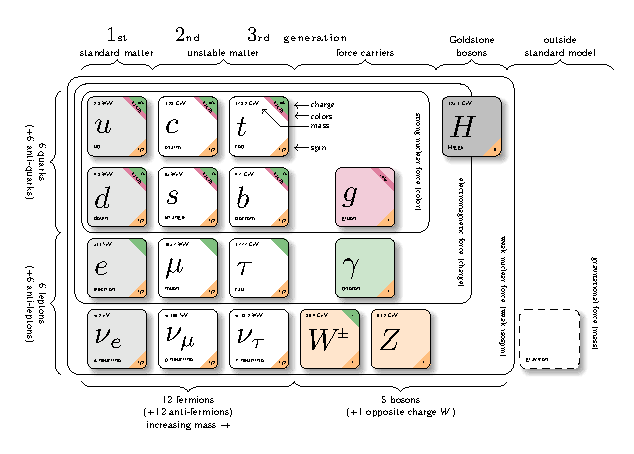
\includegraphics[width= 0.9\textwidth]{Figures/Introduction/Particles.pdf}
\caption[Diagram of the particle content of the Standard Model]{Diagram of the particle content of the \ac{SM}. For each fundamental particle, the charges, colour and spin quantum numbers are available. The measured masses for all fermions and gauge bosons are taken from Ref.~\cite{ParticleMasses} with the exception of the Higgs mass, which is taken from Ref.~\cite{Higgs_Mass}.}
\label{Figure:Introduction_1}
\end{figure}

Within the \ac{SM}, fermions serve as the fundamental constituents of all observable matter. These elementary, non-composite, spin-1/2 particles are organised into three distinct generations, with each fermion paired with an antiparticle. The antiparticles exhibit quantum numbers precisely opposite in sign, with the exception of mass and spin, which remain identical. As shown in Fig.~\ref{Figure:Introduction_1}, fermions are further divided into \textit{quarks} and \textit{leptons}. 

The leptonic sector consists of three charged leptons (\textit{electron, muon, tau}) and three electrically neutral neutrinos (\textit{electron neutrino, muon neutrino, tau neutrino}). The quark sector, on the other hand, comprises of six quark flavours; \textit{up}, \textit{down}, \textit{charm}, \textit{strange}, \textit{top} and \textit{bottom}. Within the first generation, the electron and electron neutrino comprise the leptons, while the up and down quarks form the quark sector. Although fundamental quantum numbers remain identical across generations\footnote{While fundamental quantum numbers like electric charge remain constant, others, such as flavour, vary across generations, as do properties like mass.}, the mass spectrum exhibits a strong hierarchy, with the third generation being significantly heavier than the first.

A key distinction between leptons and quarks lies in their participation in strong interactions. Unlike leptons, quarks possess an additional quantum number known as a colour charge, enabling their interactions via the strong force, which is mediated by massless gluons ($\Pg$). In addition to the strong interaction, charged leptons and quarks interact electromagnetically due to their electric charge, with massless photons ($\PGg$) acting as the mediators of the force. Conversely, neutrinos, being electrically neutral, do not participate in electromagnetic interactions. All fermions, including neutrinos, interact via the weak interaction, which occurs via the exchange of massive vector bosons, $\PW^\pm$ bosons and $\PZ$ bosons. These fundamental interactions are explored in more detail in the following section.

\section{Foundation of the fundamental interactions}
\label{Section:Chapter1_FundamentalInteractions}

Symmetries describing the fundamental interactions are the core of the \ac{SM}. N\"{o}ether's theorem~\cite{Noether_1,Noether_2}\footnote{Reference~\cite{Noether_1} is an english translation of N\"{o}ether's original paper.} shows that a conservation law is implied by the invariance of a Lagrangian under a continuous transformation (symmetry). A striking example of the deep connection between fundamental interactions and symmetry principles is the conservation of angular momentum, defined by a Lagrangian, which is invariant under rotational transformations. 

The \ac{SM} is a \textit{gauge theory} built on the principle of \textit{local gauge invariance} \ie the Lagrangian is invariant under local phase transformations. Such transformations shift the phase of the field ($\psi(x)$) as a function of the spacetime coordinates

\begin{equation_pad}
    \psi(x) \rightarrow e^{iq\theta(x)} \psi(x)
\label{Equation:Introduction_LocalPhaseTransformation}
\end{equation_pad}

where $q$ is the charge associated with the gauge symmetry and 
$\theta(x)$ is a \\ spacetime-dependent function representing the local phase transformation. The introduction of the gauge boson fields mediating fermion interactions is a direct consequence of imposing this invariance. Alone, a local phase transformation would break the invariance of the \ac{SM} Lagrangian, which is restored by the introduction of the gauge boson fields.

\subsection{Quantum Electrodynamics}
The \ac{QFT} of electromagnetism, known as \textbf{\ac{QED}}~\cite{QED}, describes the interactions between electrically charged fermions through the exchange of photons. Remarkably, the entire framework of \ac{QED} emerges beautifully from a single guiding principle: \textit{the requirement that the \ac{QED} Lagrangian remains invariant under local $\mathcal{U}$(1) gauge transformations}. The foundation of \ac{QED} begins with the Dirac equation \cite{MarkThompson} which describes the equations of motion for spin-$\frac{1}{2}$ fermion fields,

\begin{equation_pad}
    \mathcal{L}_{\text{Dirac}} = \overline{\psi}(i\gamma^\mu \partial_\mu - m_{\psi}) \psi
\label{Equation:Introduction_DiracEquation}
\end{equation_pad}

where $\psi$ and its adjoint $\overline{\psi}$ are the fermion fields expressed as four-component Dirac spinors while the quantity $\gamma^\mu$ represents the Dirac gamma matrices. Finally, $m_{\psi}$ represents the mass of the fermion.

As briefly discussed in Section~\ref{Section:Chapter1_FundamentalInteractions}, under a local $\mathcal{U}$(1) gauge transformation, the fermion field transforms in a way (Eq.~\ref{Equation:Introduction_LocalPhaseTransformation}) that breaks the local gauge invariance of the Lagrangian. Under this transformation, the Dirac equation (Eq.~\ref{Equation:Introduction_DiracEquation}) becomes

\begin{equation_pad}
    \mathcal{U}(1) \rightarrow \mathcal{L}_{\text{Dirac}}^{\prime} = \mathcal{L}_{\text{Dirac}} - q\overline{\psi}\gamma^\mu(\partial_\mu\theta(x))\psi
\label{Equation:Introduction_Dirac(U1)}
\end{equation_pad}

To restore local gauge invariance, the derivative $\partial_\mu$ is replaced with the covariant derivative $D_\mu$,

\begin{equation_pad}
    \partial_\mu \rightarrow D_\mu = \partial_\mu + iqA_\mu
\end{equation_pad}

where $A_\mu$ is a new field. The problematic term in Eq.\ref{Equation:Introduction_Dirac(U1)} can be cancelled out provided that the new field transforms as

\begin{equation_pad}
    \mathcal{U}(1) \rightarrow A_\mu^{\prime} = A_\mu - \partial_\mu \theta(x) 
\end{equation_pad}

Therefore, imposing a $\mathcal{U}$(1) local gauge invariance on the Lagrangian has forced the existence of a photon field, $A_\mu$, with well-defined gauge transformation properties. The local gauge-invariant Lagrangian for a spin-1/2 fermion field becomes

\begin{equation_pad}
    \mathcal{L}_{\text{Dirac}} = \overline{\psi}(i\gamma^\mu \partial_\mu - m_{\psi}) \psi - q\overline{\psi}\gamma^\mu A_\mu\psi
\label{Equation:Dirac_GaugeInvariant}
\end{equation_pad}

The additional term in the Lagrangian (Eq.\ref{Equation:Dirac_GaugeInvariant}) encapsulates the electromagnetic interaction between charged fermions and photons. The strength of this coupling is given by $q = |e|Q$, where e denotes the fundamental unit of electric charge, and Q represents the dimensionless charge of the fermion field $\psi$ relative to e. By N\"{o}ether's theorem, electric charge corresponds to the conserved quantity associated with a local $\mathcal{U}$(1) gauge symmetry, once again reinforcing the deep connection between symmetry and conservation laws in \ac{QFT}. The final component necessary to complete the \ac{QED} Lagrangian is the gauge-invariant kinetic term for the massless spin-1 field, described by the field strength tensor $F_{\mu\nu}$. Incorporating this, the total \ac{QED} Lagrangian takes the form,

\begin{equation_pad}
    \mathcal{L}_{\text{QED}} = \overline{\psi}(i\gamma^\mu \partial_\mu - m_{\psi}) \psi - q\overline{\psi}\gamma^\mu A_\mu\psi - \frac{1}{4}F_{\mu\nu}F^{\mu\nu}
\label{Equation:QED_GaugeInvariant}
\end{equation_pad}

\begin{equation_pad}
F_{\mu\nu} = \partial_\mu A_\nu - \partial_\nu A_\mu
\end{equation_pad}

\subsection{Quantum Chromodynamics}

The \ac{QFT} describing the strong interaction is known as \textbf{\ac{QCD}}. \ac{QCD} governs the dynamics of quarks and gluons, and \textit{it is formulated as a non-Abelian gauge theory under the local $\mathcal{SU}(3)_C$ symmetry group}. While \ac{QED} applies universally to all charged particles, the gauge symmetry of \ac{QCD} only applies to fields that carry colour charge, as denoted by the subscript $C$.

Unlike the Abelian $\mathcal{U}$(1) symmetry of \ac{QED}, which involves a single generator, the $\mathcal{SU}(3)$ symmetry group is represented by eight generators, $T^a$. To ensure local $\mathcal{SU}(3)_C$ gauge invariance, the derivative $\partial_\mu$ is replaced with the covariant derivative expressed in terms of the generators as

\begin{equation_pad}
    \partial_\mu \rightarrow D_\mu = \partial_\mu + ig_sG^{a}_{\mu}T^{a}
\end{equation_pad}

where $G^{a}_{\mu}$ represent the eight new fields, which correspond to the eight massless gluons mediating the strong interaction. The term $g_s$ encodes the coupling strength of the interaction. The full \ac{QCD} Lagrangian can then be expressed as

\begin{equation_pad} 
\mathcal{L}_{\text{QCD}} = \sum_{f}\overline{\psi_f}(i\gamma^\mu D_\mu - m_f)\psi_f - \frac{1}{4} G^{\mu\nu}_{a}G^{a}_{\mu\nu}
\end{equation_pad}

where $\psi_f$ represents the quark field (spinor) for the $f^{th}$ flavour. Once again, according to N\"{o}ether's theorem, colour charge corresponds to the conserved quantity associated with local $\mathcal{SU}(3)_C$ gauge symmetry.

Unlike \ac{QED}, the kinetic (gauge term) in the Lagrangian includes additional terms representing the self-interactions of the gauge bosons. This is a direct consequence of the \ac{QCD} generators not commuting,

\begin{equation_pad}
    [T^a,T^b] = if^{abc}T^c
\end{equation_pad}

which allows gluons themselves to carry colour charge. The quantity $f^{abc}$ refers to the structure constants of the symmetry group. This gluon self-interaction property modifies the strength of the interaction ($\alpha_{S}$), causing it to decrease as a function of the interaction energy scale. Hence, $\alpha_{S}$ is referred to as a running coupling constant.

An important consequence of this is \textit{asymptotic freedom}~\cite{AsymptoticFreedom_1,AsymptoticFreedom_2}, where at very high energies (short distances), such as the deep scattering energies at the \ac{LHC}, $\alpha_{S}$ decreases approaching zero. In this scenario, quarks and gluons behave as quasi-free particles within the protons and neutrons, allowing perturbative \ac{QCD} to describe their interactions accurately. However, at low energies, the strong coupling grows large, making \ac{QCD} non-perturbative. In this regime, quarks and gluons are not found as free particles but instead form bound, colour-neutral states known as hadrons. This phenomenon, known as \textit{colour confinement}~\cite{MarkThompson}\footnote{The phenomenon of colour confinement was first motivated theoretically in the 1970s through ideas such as flux tube formation and asymptotic freedom. A clear summary is provided in Reference~\cite{MarkThompson}.}, ensures that isolated colour-charged particles do not exist in nature; only hadrons are observed.

As a consequence of colour confinement, in high-energy collisions, high-energy quarks and gluons are observed as jets~\cite{Hadronisation_Jets} of colourless particles formed through a process known as hadronisation. In the context of proton-proton (pp) collisions, highly energetic partons fly away from the interaction point. As the partons separate, the colour field between them can be thought of as if it is being squeezed in a tube, with the energy in the field becoming increasingly larger with distance. Once that energy becomes sufficient, a new quark-antiquark pair is produced, separating the colour field into smaller segments. Eventually, the formation of colourless hadrons occurs when the quark-antiquark pairs have sufficiently low energy. This resulting cascade of collimated hadrons forms what is observed as a jet. A qualitative schematic of the hadronisation process is shown in Fig.~\ref{Figure:Introduction_ColourConfinement}.

\begin{figure}[h]
    \centering
    \begin{tikzpicture}[>=stealth,thick]

%----------------- (i) -----------------%
\node at (-2,0) {\large (i)};
% Quark & antiquark with arrows
\node[circle, fill=black, scale=0.7, label=above:$q$] (q_i) at (4.5,0) {};
\node[circle, fill=black, scale=0.7, label=above:$\bar{q}$] (qb_i) at (5.5,0) {};
\draw[->] (q_i) -- ++(-1.5, 0);
\draw[->] (qb_i) -- ++(+1.5, 0);

%----------------- (ii) -----------------%
\node at (-2,-1.5) {\large (ii)};
% Another q/qbar pair with a flux tube (string)
\node[circle, fill=black, scale=0.7, label=above:$q$] (q_ii) at (3.5,-1.5) {};
\node[circle, fill=black, scale=0.7, label=above:$\bar{q}$] (qb_ii) at (6.5,-1.5) {};
% Draw the string (solid line) plus double arrow to suggest tension
\draw[thick] (q_ii) to[out=20, in=160] (qb_ii);
\draw[thick] (q_ii) to[out=-20, in=-160] (qb_ii);
\draw (q_ii) -- (qb_ii);
\draw[->] (q_ii) -- ++(-1.5, 0);
\draw[->] (qb_ii) -- ++(+1.5, 0);

%----------------- (iii) -----------------%
\node at (-2,-3.0) {\large (iii)};
% Multiple q/qbar pairs horizontally
\node[circle, fill=black, scale=0.7, label=above:$q$] (q1_iii)  at (2.5, -3.0) {};
\node[circle, fill=black, scale=0.7, label=above:$\bar{q}$] (qb1_iii) at (4.5, -3.0) {};
\node[circle, fill=black, scale=0.7, label=above:$q$] (q2_iii)  at (5.5, -3.0) {};
\node[circle, fill=black, scale=0.7, label=above:$\bar{q}$] (qb2_iii)at (7.5, -3.0) {};

\draw[thick] (q1_iii) to[out=20, in=160] (qb1_iii);
\draw[thick] (q1_iii) to[out=-20, in=-160] (qb1_iii);
\draw[thick] (q2_iii) to[out=20, in=160] (qb2_iii);
\draw[thick] (q2_iii) to[out=-20, in=-160] (qb2_iii);

\draw (q1_iii) -- (qb1_iii);
\draw (q2_iii) -- (qb2_iii);

\draw[->] (q1_iii) -- ++(-1.5, 0);
\draw[->] (qb2_iii) -- ++(+1.5, 0);

%----------------- (iv) -----------------%
\node at (-2,-4.5) {\large (iii)};
% Multiple q/qbar pairs horizontally
\node[circle, fill=black, scale=0.7] (q11_iv)  at (1.5, -4.5) {};
\node[circle, fill=black, scale=0.7] (qb11_iv) at (2.5, -4.5) {};
\node[circle, fill=black, scale=0.7] (q12_iv)  at (3, -4.5) {};
\node[circle, fill=black, scale=0.7] (qb12_iv) at (4, -4.5) {};

\node[circle, fill=black, scale=0.7] (q21_iv)  at (5.5, -4.5) {};
\node[circle, fill=black, scale=0.7] (qb21_iv)at (6.5, -4.5) {};
\node[circle, fill=black, scale=0.7] (q22_iv)  at (7, -4.5) {};
\node[circle, fill=black, scale=0.7] (qb22_iv)at (8, -4.5) {};

\draw[thick] (q11_iv) to[out=20, in=160] (qb11_iv);
\draw[thick] (q11_iv) to[out=-20, in=-160] (qb11_iv);
\draw[thick] (q12_iv) to[out=20, in=160] (qb12_iv);
\draw[thick] (q12_iv) to[out=-20, in=-160] (qb12_iv);

\draw[thick] (q21_iv) to[out=20, in=160] (qb21_iv);
\draw[thick] (q21_iv) to[out=-20, in=-160] (qb21_iv);
\draw[thick] (q22_iv) to[out=20, in=160] (qb22_iv);
\draw[thick] (q22_iv) to[out=-20, in=-160] (qb22_iv);

\draw (q11_iv) -- (qb11_iv);
\draw (q12_iv) -- (qb12_iv);
\draw (q21_iv) -- (qb21_iv);
\draw (q22_iv) -- (qb22_iv);

\draw[->] (q11_iv) -- ++(-1.5, 0);
\draw[->] (qb22_iv) -- ++(+1.5, 0);
%----------------- (v) -----------------%
\node at (-2,-6.5) {\large (v)};
% Final hadrons on the left
\node[draw, circle, scale=1.0] (H1_v) at (1.5,-6) {};
\node[draw, circle, scale=1.0] (H2_v) at (1.7,-7) {};
\node[draw, circle, scale=1.0] (H3_v) at (2.5,-6.2) {};
\node[draw, circle, scale=1.0] (H4_v) at (2,-6.4) {};

% Arrows indicating motion outward
\draw[->] (1.2,-6) -- ++(-0.7, 0.6);
\draw[->] (1.2,-6.2) -- ++(-0.7, 0.4);
\draw[->] (1.2,-6.4) -- ++(-0.7, 0.2);
\draw[->] (1.2,-6.6) -- ++(-0.7, -0.2);
\draw[->] (1.2,-6.8) -- ++(-0.7, -0.4);
\draw[->] (1.2,-7) -- ++(-0.7, -0.6);

% Final hadrons on the right
\node[draw, circle, scale=1.0] (H5_v) at (8,-6) {};
\node[draw, circle, scale=1.0] (H6_v) at (7.8,-7) {};
\node[draw, circle, scale=1.0] (H7_v) at (7,-6.2) {};
\node[draw, circle, scale=1.0] (H8_v) at (7.5,-6.4) {};
\draw[->] (8.3,-6) -- ++(0.7, 0.6);
\draw[->] (8.3,-6.2) -- ++(0.7, 0.4);
\draw[->] (8.3,-6.4) -- ++(0.7, 0.2);
\draw[->] (8.3,-6.6) -- ++(0.7, -0.2);
\draw[->] (8.3,-6.8) -- ++(0.7, -0.4);
\draw[->] (8.3,-7) -- ++(0.7, -0.6);

\end{tikzpicture}
    \caption{Qualitative schematic of the steps involved in the hadronisation process.}
    \label{Figure:Introduction_ColourConfinement}
\end{figure}

\subsection{Electroweak theory}

In the 1960s, Glashow~\cite{Glashow_1}, Salam~\cite{Salam_1} and Weinberg~\cite{Weinberg_1} discovered that \textit{a unified picture of the electromagnetic and weak interactions} could be constructed. They proposed to develop the electroweak theory incorporating the characteristics of both interactions by associating them with the $\mathcal{SU}(2)_{L}$ $\otimes$ $\mathcal{U}(1)_{Y}$ symmetry group,

\begin{equation_pad}
    \mathcal{SU}(2)_L \otimes \mathcal{U}(1)_Y \rightarrow \mathcal{L}^{\prime}_{\text{EW}} = \mathcal{L}_{\text{EW}}
\end{equation_pad}

where $L$ denotes the \textit{left-handed nature} of the weak interaction under $\mathcal{SU}(2)_L$, and $Y$ represents the \textit{weak hypercharge} associated with the $\mathcal{U}(1)_Y$ gauge symmetry. To ensure that the electroweak Lagrangian is invariant under local transformations of this symmetry group, the covariant derivative is written as

\begin{equation_pad}
    D_\mu = \partial_\mu + \underbrace{ig^{\prime}B_\mu Y}_{\mathcal{U}(1)_Y} + \underbrace{\frac{i}{2}gW^i_\mu\sigma^i}_{\mathcal{SU}(2)_L}
\end{equation_pad}

where $Y$ is the single generator of the $\mathcal{U}(1)_Y$ gauge group, associated with the gauge boson field, $B_\mu$. While the three generators of $\mathcal{SU}(2)_L$ are represented by the 2 x 2 Pauli-spin matrices ($\sigma^i$), associated with the three gauge boson fields, $W^i_\mu$. The coupling strengths of the interactions are represented by $g$ and $g^{\prime}$, respectively. The conserved charges corresponding to these gauge symmetries are the weak isospin component, $I_3$, for $\mathcal{SU}(2)_L$ and the weak hypercharge, Y, for $\mathcal{U}(1)_Y$.

By imposing gauge invariance under the electroweak symmetry group, four gauge fields arise: the three weak isospin fields, $W_{\mu}^{(i)}$ (i=1,2,3), and the weak hypercharge field, $B_{\mu}$. These gauge fields can be expressed in terms of the physical bosons as,

\begin{equation_pad}
\begin{array}{c}
A_{\mu} = + B_{\mu} \cos{\theta_{W}} + W_{\mu}^{(3)} \sin{\theta_{W}}, \\
Z_{\mu} = - B_{\mu} \sin{\theta_{W}} + W_{\mu}^{(3)} \cos{\theta_{W}}, \\
W_{\mu}^{\pm} = \frac{1}{\sqrt{2}} (W_{\mu}^{(1)} \mp iW_{\mu}^{(2)}),
\end{array}
\label{Equation:Introduction_PhysicalGaugeFields}
\end{equation_pad}

where $\theta_{W}$, the weak mixing angle, quantifies the mixing between the weak isospin and hypercharge gauge fields. It is related to the weak and electromagnetic coupling constants, $g$ and $g^{\prime}$, by

\begin{equation_pad}
    \theta_W = \text{arctan}(\frac{g^{\prime}}{g})
\end{equation_pad}

As discussed earlier in Section~\ref{Section:Particle content and fundamental interactions}, all fermions interact via the weak interaction. A key feature of the weak interaction is its violation of parity symmetry~\cite{ParityViolation_Wu}. This means that weak interactions exhibit different behaviours under spatial inversions. In contrast to \ac{QED} and \ac{QCD}, which conserve parity and involve pure vector interactions of the form,

\begin{equation_pad}
    j^\mu = \overline{u}\gamma^\mu u
\end{equation_pad}

the weak interaction is required to take a different form to account for its parity-violating nature.

Mathematically, the proper parity transformations can be achieved by requiring the interaction to have a chiral structure. Naturally, this leads to either a V-A or V+A (Vector, Axial Vector) current. Experimentally, it is well established that the weak interaction exhibits a V-A charged current of the form,

\begin{equation_pad}
    j^\mu_{\text{weak}} = \overline{u}\gamma^\mu \frac{1}{2}(1-\gamma^5)u
\label{Equation:Chapter1-WeakChargedCurrent}
\end{equation_pad}

Using chiral operators, $P_{L/R}$, the fermion spinor fields ($u$) can be decomposed into left-handed ($u_{L}$) and right-handed ($u_{R}$) chiral components. 

\begin{equation_pad}
\begin{array}{c}
    P_{L/R} = \frac{1}{2}(1\mp \gamma^5) \quad ,\quad \gamma^5 = \gamma^0\gamma^1\gamma^2\gamma^3 \\
    u = P_Ru +P_Lu = u_R + u_L
\end{array}
\end{equation_pad}

This chiral decomposition is fundamental in the EW theory, only allowing interactions between left-handed fermions (and equivalently, right-handed anti-fermions) and the weak isospin gauge bosons $W_{\mu}^{(i)}$. This can be explicitly seen by substituting the decomposed spinor field ($u$) into the weak charged current (Eq.~\ref{Equation:Chapter1-WeakChargedCurrent}),

\begin{equation_pad}
\begin{array}{c}
    j^\mu_{\text{weak}} = (\overline{u_R} + \overline{u_L})\gamma^\mu P_L (u_R+u_L) \\
    P_L u_R = 0
\label{Equation:Chapter1-WeakChargedCurrent_Decomposed}
\end{array}
\end{equation_pad}

Hence, in this representation, it is natural that the left-handed components of the fermion fields transform as doublets under $\mathcal{SU}(2)_L$. Conversely, the right-handed components transform as singlets and do not interact with the charged weak gauge bosons. This structure of the EW theory leads to a relationship between the weak isospin, weak hypercharge and electric charge.

\begin{equation_pad}
    Q = I_3 + \frac{Y}{2}
\end{equation_pad}

where this equation beautifully encapsulates how the EW symmetry unifies the electromagnetic and weak interactions, allowing for a calculation of the charge of all fundamental particles.

Despite beautifully unifying the electromagnetic and weak interactions into a single theory, a fundamental issue persists because of non-zero mass measurements of the $\PW$ and $\PZ$ bosons~\cite{W_Z_MassMeasurements_1,W_Z_MassMeasurements_2}. This is clearly omitted from the EW Lagrangian, as including the required terms would break the underlying gauge symmetry. Mass terms of the form ${m_{W}^2 W_{\mu}^{-} W^{+\mu}}$ and $\frac{1}{2} m_{Z}^{2} Z_{\mu} Z^{\mu}$ are not invariant under the $\mathcal{SU(2)}_{L}$ $\otimes$ $\mathcal{U}(1)_{Y}$ symmetry group. This also extends to fermions with mass terms of the form, $m\overline{\psi}\psi = m(\overline{\psi}_{R}\psi_{L} + \overline{\psi}_{L}\psi_{R})$. The inclusion of such a term in the EW Lagrangian would break the symmetry because of left-handed and right-handed chiral components transform differently. The answer to this puzzle came through the Higgs mechanism, which is discussed in Section~\ref{Section:Introduction_HiggsMechanism}.

\section{Brout-Englert-Higgs mechanism}
\label{Section:Introduction_HiggsMechanism}
First proposed back in the 1960s by Englert and Brout~\cite{Englert_Brout}, Higgs~\cite{PeterHiggs_1,PeterHiggs_2,PeterHiggs_3}, and Guralnik, Hagen and Kibble~\cite{Guralnik_Hagen_Kibble,Kibble}, the \textbf{\ac{BEH} mechanism} provides a way to generate mass while preserving the local gauge invariance of the \ac{SM}. It is based on the principle of \textbf{\ac{SSB}}~\cite{SSB_Definition} where \textit{the Lagrangian of a system remains invariant under a certain symmetry group, but the vacuum state of the system does not}. The symmetry of the \ac{SM} Lagrangian is broken through the \ac{BEH} mechanism as

\begin{equation_pad}
    \mathcal{SU}(3)_C \otimes \mathcal{SU}(2)_L \otimes \mathcal{U}(1)_Y \quad \underbrace{\rightarrow}_{\text{BEH}} \quad \mathcal{SU}(3)_C \otimes \mathcal{U}(1)_{\text{EM}}
\end{equation_pad}

Effectively, the \ac{BEH} mechanism targets and breaks the symmetry of the electroweak interaction. This symmetry is broken by introducing two complex scalar fields, $\phi^{+/0}$, which transform as a doublet $\Phi$ under $SU(2)_L$ transformations,

\begin{equation_pad}
\Phi =
\begin{pmatrix}
\phi^{+} \\
\phi^{0} 
\end{pmatrix}
= \frac{1}{\sqrt{2}} \begin{pmatrix}
    \phi_{1} + i\phi_{2} \\
    \phi_{3} + i\phi_{4}
\end{pmatrix}
\end{equation_pad}

This doublet, known as the Higgs field, contributes four \ac{dof} to the \ac{SM} Lagrangian; one for the real part and one for the imaginary part of each component. The corresponding Lagrangian for the Higgs field is

\begin{equation_pad}
    \mathcal{L}_{\text{Higgs}} = (D_{\mu} \Phi)^{\dagger}(D^{\mu}\Phi) - \underbrace{(\mu^{2}\Phi^{\dagger}\Phi + \lambda(\Phi^{\dagger}\Phi)^2)}_{\text{V($\Phi$)}}
\label{Equation:Introduction_HiggsLagrangian}
\end{equation_pad}

where $D_{\mu}$ is the covariant derivative,

\begin{equation_pad}
    D_{\mu} = \partial_{\mu} + i\frac{g}{2}\vec{T}\cdot\vec{W_{\mu}} + i\frac{g'}{2}YB_{\mu}
\end{equation_pad}

The second term in Eq.~\ref{Equation:Introduction_HiggsLagrangian} represents the Higgs potential shown in Fig.~\ref{Figure:Introduction_HiggsPotential}, which depends on the Higgs field and two real parameters, $\mu^{2}$ and $\lambda$. The vacuum state of the Higgs field corresponds to the minimum of this potential, imposing constraints on these parameters. To ensure a finite minimum, $\lambda$ must be positive ($\lambda > 0$), but no such restriction applies to $\mu^{2}$. For $\mu^{2} > 0$, the potential has a single symmetric minimum at zero \ac{VEV}. Conversely, for $\mu^{2} < 0$, the potential develops an infinite set of minima, leading to \ac{SSB}  via the \ac{BEH} mechanism. In this case, the Higgs field satisfies,

\begin{figure}[h]
\centering
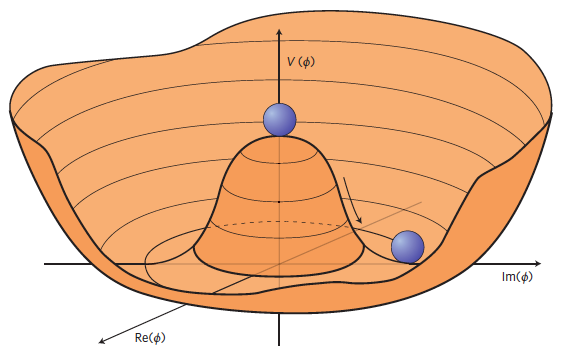
\includegraphics[width= .7\textwidth]{Figures/Introduction/higgspotential.png}
\caption[Form of the Higgs potential.]{Form of the Higgs potential giving rise to \ac{SSB} via the \ac{BEH} mechanism. Figure taken from Ref~\cite{HiggsPotential}.}
\label{Figure:Introduction_HiggsPotential}
\end{figure}

\begin{equation_pad}
    \Phi^{\dagger}\Phi = -\frac{\mu^{2}}{2\lambda} = \frac{\nu^2}{2}
\end{equation_pad}

A key constraint to achieving \ac{SSB} through the \ac{BEH} mechanism is to ensure that the photon remains massless while the other gauge bosons acquire mass. Hence, the Higgs potential's minimum must correspond to a nonzero \ac{VEV} exclusively for the neutral scalar field, $\phi^{0}$. This condition preserves the $\mathcal{U}(1)_{\text{EM}}$ symmetry after \ac{SSB}.

\begin{equation_pad}
    <0|\Phi|0> = \frac{1}{\sqrt{2}} \begin{pmatrix}
        0 \\
        \nu
    \end{pmatrix}
\end{equation_pad}
 
Before expanding the Higgs field around its minimum to study the consequences of \ac{SSB}, it is important to recall \textbf{Goldstone's theorem}~\cite{Goldstone}. \textit{This theorem predicts the emergence of a massless scalar (Goldstone) boson after the spontaneous breaking of a continuous symmetry}. Out of the four \ac{dof} introduced by the Higgs field, the three associated with the broken symmetry generators become Goldstone bosons, which appear as massless scalar fields in the Lagrangian. Gauge invariance guarantees that the choice of gauge does not affect the physical predictions of the theory, allowing us to eliminate the Goldstone bosons from the Lagrangian by making an appropriate local gauge transformation. This is referred to as the unitary gauge, where the \ac{dof} associated with the massless Goldstone bosons are replaced with new \ac{dof} corresponding to the longitudinal polarisation states of the gauge bosons ($\PW^{\pm}/\PZ$). In the unitary gauge, the Higgs field can be re-expressed as,

\begin{equation_pad}
    \text{BEH} \rightarrow \Phi = \frac{1}{\sqrt{2}}\begin{pmatrix}
        0 \\
        \nu + h
    \end{pmatrix} 
    \label{Equation:Introduction_HiggsField_2}
\end{equation_pad}

where h is the physical Higgs field, the fourth \ac{dof} in the Higgs sector.

The term in the Lagrangian responsible for the generation of the masses of gauge bosons is $(D_\mu\Phi)^\dagger(D^\mu\Phi)$. Substituting Eq.~\ref{Equation:Introduction_HiggsField_2} into this term and expressing the $B_\mu$ and $W_{\mu}^{(i)}$ fields in terms of physical $Z_\mu$ and $W_{\mu}^{\pm}$ states using Eq.~\ref{Equation:Introduction_PhysicalGaugeFields}, we obtain the following weak boson mass terms,

\begin{equation_pad}
    \text{BEH} \rightarrow \mathcal{L}_{\text{Higgs}} \supset \frac{1}{4} g^2 \nu^2 W^{+\mu}W_{\mu}^- + \frac{(g^2+g'^2)\nu^2}{8} Z_\mu Z^\mu
\label{Equation:Introduction_HiggsLagrangian_2}
\end{equation_pad}

Using the known form of a mass term for a spin-1 gauge boson, the masses of the $W^\pm$ and the Z bosons can be expressed in terms of the $\mathcal{SU}(2)_{L}$ $\otimes$ $\mathcal{U}(1)_{Y}$ gauge couplings and the Higgs \ac{VEV} ($\nu = 246 \GeV$) as,

\begin{equation_pad}
\begin{aligned}
    m_W &= \frac{1}{2}g\nu \\
    m_Z &= \frac{1}{2}\nu\sqrt{g^2+g'^2}\\
\end{aligned}
\end{equation_pad}

Importantly, in this physical basis, the neutral gauge boson associated with the $\text{A}_\mu$ field remains massless while the physical Higgs field also appears in the Lagrangian with the associated terms being,

\begin{equation_pad}
    \text{BEH} \rightarrow \mathcal{L}_{\text{Higgs}} \supset \underbrace{\frac{1}{2} \partial_\mu h \, \partial^\mu h - \lambda \nu^2 h^2}_{\text{massive scalar boson } h}
    \underbrace{- \lambda \nu h^3 - \frac{1}{4} \lambda h^4}_{\text{Higgs self-interactions}}
\label{Equation:Introduction_HiggsLagrangian_3}
\end{equation_pad}

According to Eq.~\ref{Equation:Introduction_HiggsLagrangian_3}, the mass of the scalar boson field in given by $\text{m}_H = \sqrt{2\lambda}\nu$. This Lagrangian also contains terms describing the trilinear and quartic self-interactions of the Higgs boson for which the relevant Feynman diagrams are shown in Fig.~\ref{Figure:Introduction_HiggsSelf}. While only the self-interaction terms are shown in Eq.~\ref{Equation:Introduction_HiggsLagrangian_3}, the Lagrangian also contains interaction terms between the Higgs boson and the weak gauge bosons ($\PW^\pm/\PZ$). 

\begin{figure}[h]
    \centering
    % First row
    \begin{subfigure}{0.45\textwidth}
        \centering
        \begin{tikzpicture}
    \begin{feynman}
        \vertex[blue] at (0, 0) (a) {\(H\)};
        \vertex at (2, 0) (center);
        \vertex[blue] at (4, 1.5) (b) {\(H\)};
        \vertex[blue] at (4, -1.5) (c) {\(H\)};

        \diagram*{
            (a) -- [scalar] (center),
            (center) -- [scalar] (b),
            (center) -- [scalar] (c),
        };
    \end{feynman}
\end{tikzpicture}


    \end{subfigure}
    \hfill
    \begin{subfigure}{0.45\textwidth}
        \centering
        \begin{tikzpicture}
    \begin{feynman}
        \vertex[blue] at (0, 1.5) (a) {\(H\)};
        \vertex[blue] at (0, -1.5) (a1) {\(H\)};

        \vertex at (2, 0) (center);
        \vertex[blue] at (4, 1.5) (b) {\(H\)};
        \vertex[blue] at (4, -1.5) (c) {\(H\)};

        \diagram*{
            (a) -- [scalar] (center),
            (a1) -- [scalar] (center),
            (center) -- [scalar] (b),
            (center) -- [scalar] (c),
        };
    \end{feynman}
\end{tikzpicture}


    \end{subfigure}
    \caption[Feynman diagrams from Higgs self-interactions in the Standard Model]{Feynman diagrams arising from the presence of the Higgs self-interaction terms in the \ac{SM} Lagrangian.}
    \label{Figure:Introduction_HiggsSelf}
\end{figure}

Remarkably, fermions in the \ac{SM} also acquire masses via the \ac{BEH} mechanism through Yukawa interactions. After \ac{SSB}, when the Higgs field acquires a \ac{VEV}, the Yukawa part of the Lagrangian takes the form

\begin{equation_pad}
    \text{BEH} \rightarrow \mathcal{L}_{\text{Yukawa}}^f = \underbrace{-\frac{g_f}{\sqrt{2}}\nu(\overline{\psi_L}\psi_R + \overline{\psi_R} \psi_L)}_{\text{mass term}} \underbrace{- \frac{g_f}{\sqrt{2}}h(\overline{\psi_L}\psi_R + \overline{\psi_R} \psi_L)}_{\text{interaction term}}
\label{Equation:Introduction_YukawaLagrangian}
\end{equation_pad}

where $\psi_L$ and $\psi_R$ are the left-handed and right-handed chiral fields, and the first term gives the fermionic mass $m_f = g_f\nu / \sqrt{2}$. The second term in the Lagrangian describes the coupling between the fermion and the Higgs boson itself, interestingly indicating that heavier fermions couple stronger to the Higgs.

\section{The Higgs boson}

Undoubtedly, one of the most significant achievements in modern physics is the observation of the long-sought fundamental boson, the Higgs. The confirmation of its existence came in 2012, when the ATLAS and \ac{CMS} Collaborations~\cite{Higgs_ATLAS,Higgs_CMS} jointly announced its discovery, marking the completion of the \ac{SM} particle content. Soon after its discovery, both collaborations conducted several measurements exploring the properties of the Higgs, demonstrating that the observed Higgs looks very much like the \ac{SM} Higgs~\cite{HiggsParity_1,HiggsParity_2}. One important test lies in the Higgs boson couplings. The most recent measurements of the coupling strengths~\cite{CMS_Couplings_Measurement} are consistent with the \ac{SM} prediction, as presented in Fig.~\ref{Figure:Introduction_CMScouplings}.

\begin{figure}[h]
\centering
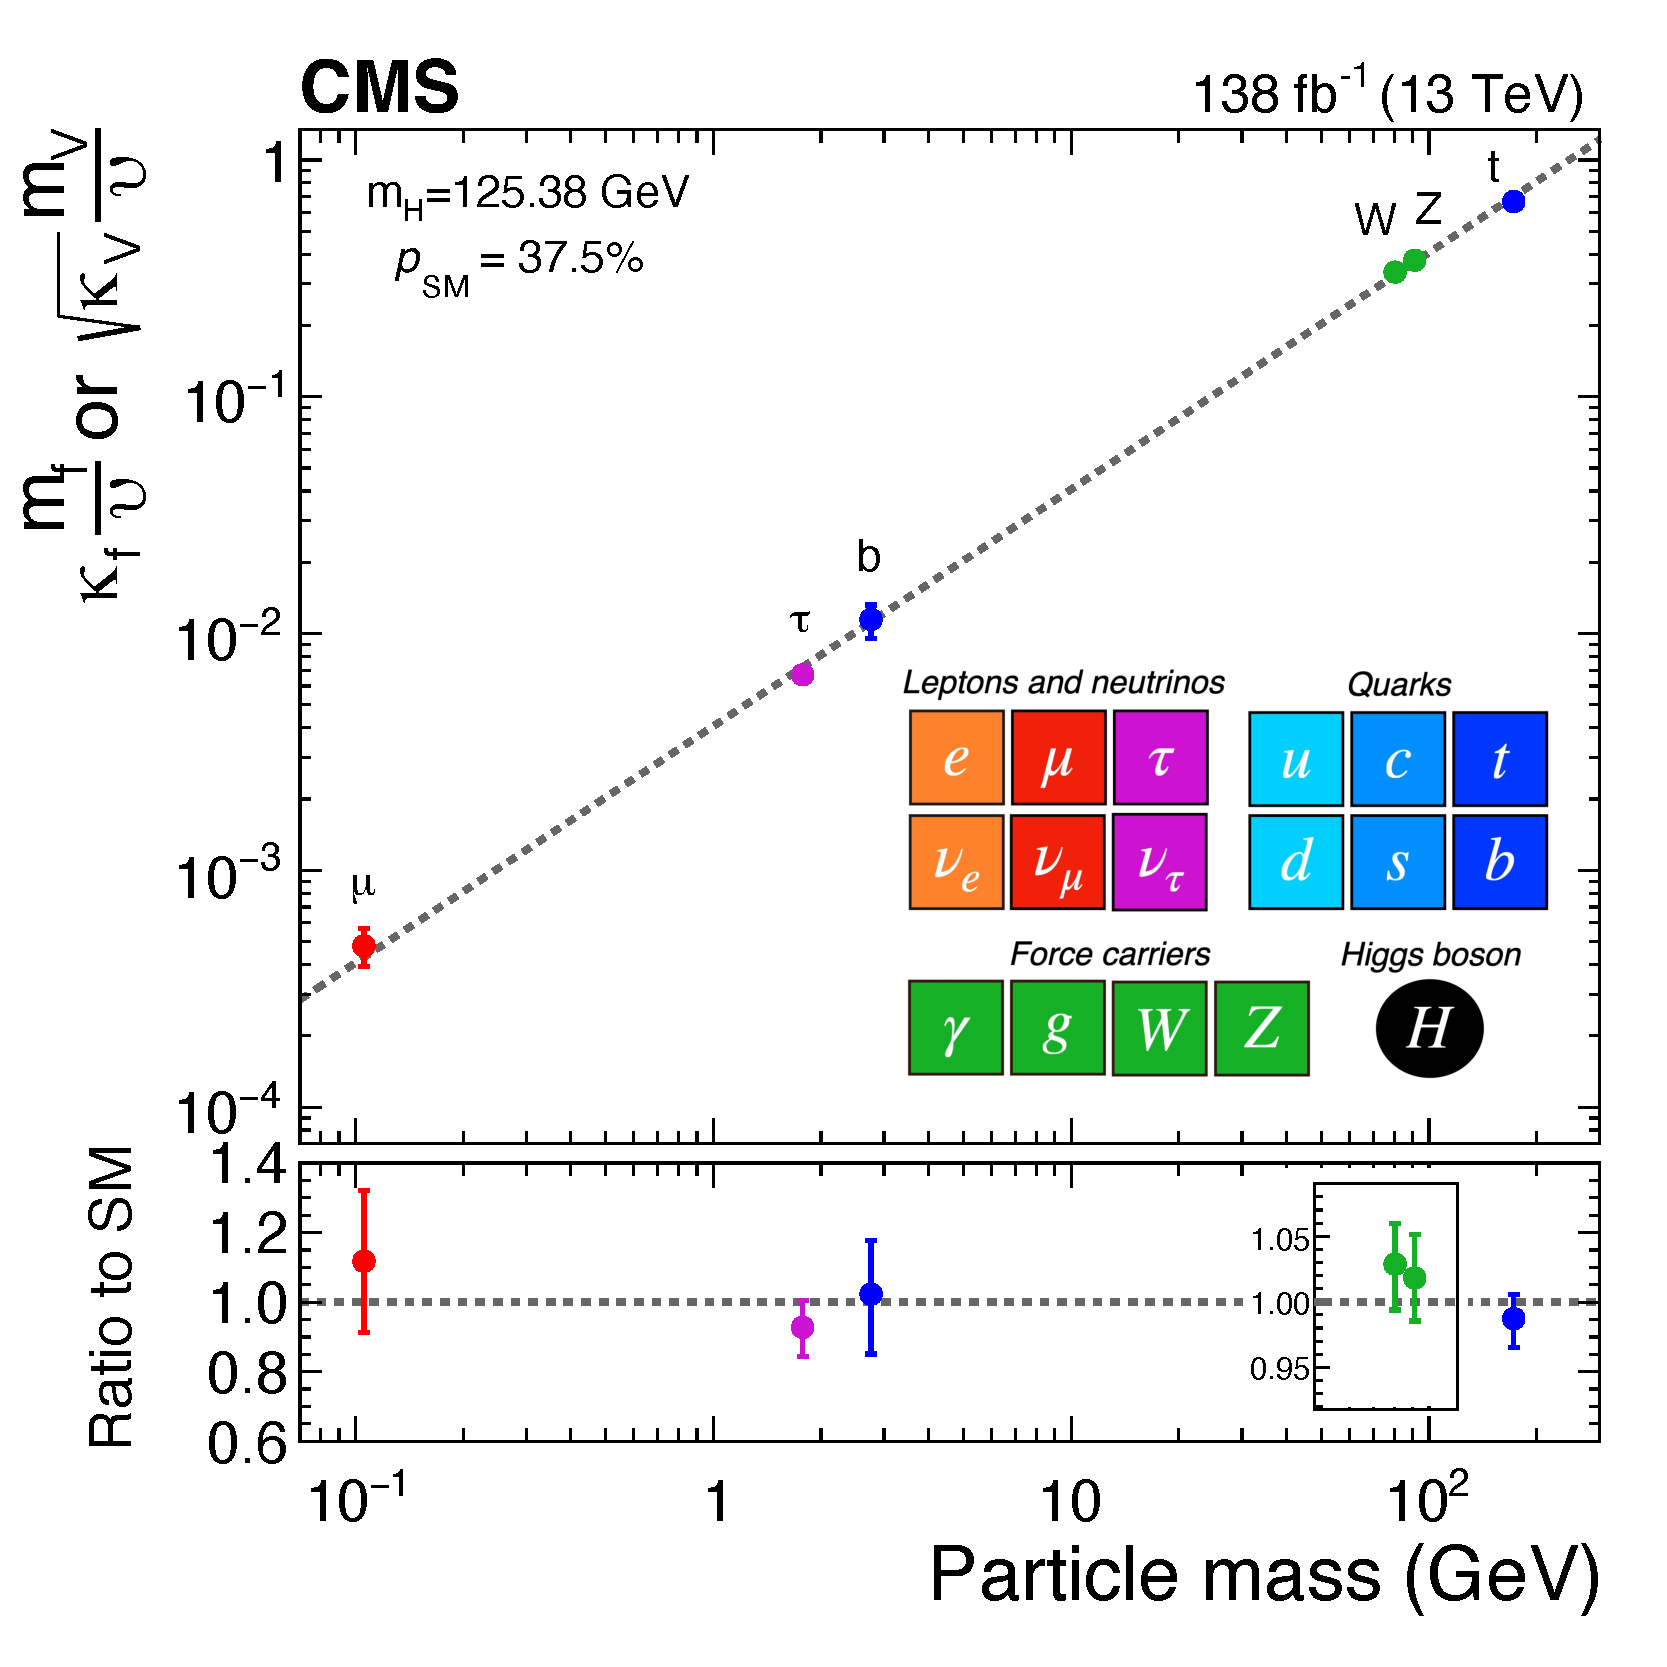
\includegraphics[width= .7\textwidth]{Figures/Introduction/CMS_Higgs_FermionCouplings.pdf}
\caption[Measured Higgs coupling modifiers versus fermion and boson masses]{The measured coupling strength modifiers of the Higgs boson to fermions and heavy gauge bosons are presented as a function of the fermionic/bosonic masses. For gauge bosons, the ``reduced" coupling modifiers are presented to keep a linear proportionality to the mass. Figure taken from Ref.~\cite{CMS_Couplings_Measurement}.}
\label{Figure:Introduction_CMScouplings}
\end{figure}

\subsection{Higgs boson production}

At the \ac{LHC}, the Higgs boson is produced via four major production modes: \textit{\ac{ggH}}, \textit{\ac{VBF}}, \textit{\ac{VH}}, and \textit{$t\overline{t}$-associated production} (ttH); listed in order of decreasing cross-section. In addition to the dominant production modes, the Higgs can still be produced in different ways \eg \textit{in association with a single-top} (tH). The Feynman diagrams of the dominant modes are displayed in Fig.~\ref{Figure:Introduction_HiggsProductionModes} while their respective cross-sections at $\sqrt{s}$ = 13$\TeV$ and $\sqrt{s}$ = 13.6$\TeV$ are displayed in Table~\ref{Table:Introduction_HiggsProduction_XS}. 


\begin{figure}[h]
    \centering
    % First row
    \begin{subfigure}{0.45\textwidth}
        \centering
        \begin{tikzpicture}
    \begin{feynman}
        \vertex at (0, 1.5) (i1) {\(g\)};
        \vertex at (0,-1.5) (i2) {\(g\)};
        \vertex at (2.5, 1.5) (a);
        \vertex at (2.5,-1.5) (b);
        \vertex at (4, 0) (c);
        \vertex[blue] at (6, 0) (f) {\(H\)};
        \vertex at (3.25,0) () {\(t\)};
        \diagram*{
            (i1) -- [gluon] (a),
            (i2) -- [gluon] (b),
            (a) -- [fermion] (b) -- [fermion] (c) -- [fermion] (a),
            (c) -- [scalar] (f),
        };
    \end{feynman}
\end{tikzpicture}


        \caption{ggH}
    \end{subfigure}
    \hfill
    \begin{subfigure}{0.45\textwidth}
        \centering
        \begin{tikzpicture}
    \begin{feynman}
        \vertex at (0, 1.) (i1) {\(q\)};
        \vertex at (0,-1.) (i2) {\(q\)};

        \vertex at (3, 1) (a);
        \vertex at (3,-1) (b);
        \vertex at (4,0) (c);

        \vertex[blue] at (6, 0) (f) {\(H\)};
        \vertex at (6, 1.5) (e) {\(q\)};
        \vertex at (6,-1.5) (g) {\(q\)};

        \vertex at (4.25,0.6) () {\(W/Z\)};
        \vertex at (4.25,-0.6) () {\(W/Z\)};

        \diagram*{
            (i1) -- [fermion] (a),
            (i2) -- [fermion] (b),
            (a) -- [photon] (c),
            (b) -- [photon] (c),
            (c) -- [scalar] (f),
            (a) -- [fermion] (e),
            (b) -- [fermion] (g),
        };
    \end{feynman}
\end{tikzpicture}
        \caption{VBF}
    \end{subfigure}

    % Add vertical space between rows
    \vspace{0.5cm}

    % Second row (centered properly)
    \begin{subfigure}{0.45\textwidth}
        \centering
        \raisebox{-5mm}{\begin{tikzpicture}
    \begin{feynman}
        \vertex at (0, 1.5) (i1) {\(q\)};
        \vertex at (0,-1.5) (i2) {\(\overline{q}\)};

        \vertex at (2,0) (a);
        \vertex at (4, 0) (b);

        \vertex at (6.15, 1.5) (c) {\(W/Z\)};
        \vertex[blue] at (6,-1.5) (d) {\(H\)};

        \vertex at (3,0.25) () {\(W/Z\)};

        \diagram*{
            (i1) -- [fermion] (a) -- [fermion] (i2),
            (a) -- [photon] (b),
            (b) -- [photon] (c),
            (b) -- [scalar] (d),
        };
    \end{feynman}
\end{tikzpicture}}
        \caption{WZ associated}
    \end{subfigure}
    \hfill
    \begin{subfigure}{0.45\textwidth}
        \centering
        \begin{tikzpicture}
    \begin{feynman}
        \vertex at (0, 1.5) (i1) {\(g\)};
        \vertex at (0,-1.5) (i2) {\(g\)};
        
        \vertex at (3, 1.5) (a);
        \vertex at (3,0) (ab);
        \vertex at (3,-1.5) (b);
        
        \vertex at (6, 1.5) (c) {\(\overline{t}\)};
        \vertex at (6, -1.5) (d) {\(t\)};

        \vertex[blue] at (6, 0) (f) {\(H\)};

        \diagram*{
            (i1) -- [gluon] (a),
            (i2) -- [gluon] (b),
            (c) -- [fermion] (a),
            (a) -- [fermion] (ab),
            (ab) -- [fermion] (b),
            (b) -- [fermion] (d),
            (ab) -- [scalar] (f),
        };
    \end{feynman}
\end{tikzpicture}


        \caption{$t\bar{t}$ associated}
    \end{subfigure}

    \caption{Feynman diagrams of the main Standard Model Higgs production modes at the Large Hadron Collider.}
    \label{Figure:Introduction_HiggsProductionModes}
\end{figure}


\begin{table}[htbp]
\centering
\renewcommand{\arraystretch}{1.5} % Increase row height
\arrayrulecolor{black} % Ensure outer border is black
\begin{tabular}{|c|c|c|}
\hline
Mechanism & Cross Section @ 13 TeV [pb] & Cross Section @ 13.6 TeV [pb] \\ \hline \hline 
ggH                                & 48.60  & 52.23 \\ 
\arrayrulecolor{lightgray} \hline
VBF                                & 3.78  & 4.08 \\ 
\arrayrulecolor{lightgray} \hline
WH                                 & 1.37  & 1.46 \\ 
\arrayrulecolor{lightgray} \hline
ZH                                 & 0.76  & 0.94 \\ 
\arrayrulecolor{lightgray} \hline
ttH                                & 0.51  & 0.57 \\ 
\arrayrulecolor{black} \hline
\end{tabular}
\caption[Cross sections of dominant Standard Model Higgs production modes at $13$ and $13.6\TeV$]{Cross sections of the dominant Higgs production mechanisms in the \ac{SM}. Derived for $\text{m}_H = 125\GeV$ and presented for both $\sqrt{s}=13\TeV$ and $\sqrt{s}=13.6\TeV$~\cite{HiggsProduction_XS_13TeV,HiggsProduction_XS_13p6TeV}.}
\label{Table:Introduction_HiggsProduction_XS}
\end{table}

The ggH production mode is the most dominant, proceeding via an internal quark loop. This is a consequence of the Higgs not directly coupling to the gluon. Despite its dominance, other production modes, such as VBF, have an interesting feature: additional objects in their final states. These distinct topologies can be leveraged to reduce backgrounds. In particular, the VBF production mode is characterised by two additional energetic jets, which tend to have a large spatial separation and a high invariant mass.

\subsection{Higgs boson decays}

The Higgs boson is an unstable particle, decaying almost immediately after its production~\cite{MarkThompson}, with its inference only possible from the decay products. The dominant \ac{SM} Higgs decays channels are listed in Table~\ref{Table:Introduction_HiggsBranchingFractions}, clearly showing that $H\rightarrow b\overline{b}$ is the dominant decay mode. 

\begin{table}[h]
\centering
\renewcommand{\arraystretch}{1.5} % Increase row height
\setlength{\tabcolsep}{12pt} % Increase column width
\arrayrulecolor{black} % Ensure outer border is black
\begin{tabular}{|c|c|}
\hline
Decay Mode                  & Branching Fraction {[}\%{]} \\ \hline \hline
$b\overline{b}$             & 58.24 \\ 
\arrayrulecolor{lightgray} \hline
$WW^*$                      & 21.37 \\ 
\arrayrulecolor{lightgray} \hline
$gg$                        & 8.19  \\ 
\arrayrulecolor{lightgray} \hline
$\tau\tau$                  & 6.27  \\ 
\arrayrulecolor{lightgray} \hline
$c\overline{c}$             & 2.89  \\ 
\arrayrulecolor{lightgray} \hline
$ZZ^*$                      & 2.61  \\ 
\arrayrulecolor{lightgray} \hline
$\gamma\gamma$              & 0.23  \\ 
\arrayrulecolor{lightgray} \hline
$\mu\mu$                    & 0.02  \\ 
\arrayrulecolor{black} \hline
\end{tabular}
\caption[Branching fractions of main Standard Model Higgs decay channels at $\text{m}_H = 125\GeV$]{Branching fractions, $\text{B}_f$, of the main \ac{SM} Higgs boson decay channel for $\text{m}_H = 125\GeV$~\cite{HiggsProduction_XS_13TeV,HiggsProduction_XS_13p6TeV} where for a particular final state $f$, $\text{B}_f = \Gamma_f/\Gamma_H$, with $\Gamma_f$ and $\Gamma_H$ being the decay width of the final state and the Higgs boson respectively.}
\label{Table:Introduction_HiggsBranchingFractions}
\end{table}

However, the sensitivity of this mode is heavily impacted by the presence of a large hadronic background. The Higgs discovery was only possible after a combination of several of the decay channels; $H\rightarrow ZZ \rightarrow 4l$, $H\rightarrow \gamma \gamma$, $H\rightarrow WW^*$, $H\rightarrow \tau\tau$ and $H\rightarrow b\overline{b}$, with the di-photon and four lepton decay channels being the main contributors. Particularly interesting is the $H\rightarrow \tau\tau$ decay mode, providing a relatively large branching fraction while being less impaired by backgrounds than $H\rightarrow b\overline{b}$.

\setcounter{mtc}{2}
\chapter{Motivation for Higgs Sector Extensions and Higgs CP Studies}
\chaptermark{Motivation for Higgs Sector Extensions and Higgs CP Studies}  
\thispagestyle{plain}  % First page has default style
\pagestyle{chapterpages}
\label{Section:Chapter2}

In Chapter~\ref{Section:Chapter1}, the SM of particle physics was explored to establish the theoretical foundation of this work. While the SM has been immensely successful, with its predictions verified experimentally to a high degree of precision, it remains an incomplete theory of nature due to several fundamental theoretical problems. Beyond these theoretical issues, the emergence of experimental results in tension with SM predictions has sparked significant interest among particle physicists. Although the statistical significance of these tensions is not yet sufficient to claim new discoveries, the search for BSM physics to explain them remains an intriguing and active area of research. This chapter will focus on two major theoretical challenges; the hierarchy problem and the observed matter-antimatter asymmetry of the universe, while also briefly discussing key experimental tensions. Possible solutions within the context of BSM physics will then be explored, with the observed Higgs boson playing an integral role in the matter-antimatter asymmetry discussion.

\section{Hierarchy problem}
With these fundamental problems in mind, it seems fairly clear that the SM is an \ac{EFT}, describing physics up to a certain energy scale. However, an extension is required to describe physics at the Planck scale ($10^{19}\GeV$) where gravitational effects become significant. The hierarchy problem is a central issue in the Higgs sector arising from the absence of a natural mechanism to stabilise the Higgs mass against large quantum corrections.

In QFT, the Higgs boson mass in not simply a fixed parameter, receiving corrections to its physical mass from virtual processes involving particles that couple directly or indirectly to the Higgs field. Mathematically the physical mass of the Higgs boson can be expressed as

\begin{equation}
    m_H^2 = (m_H^0)^2 + \Delta m_H^2
\label{Equation:Chapter2_HiggsBosonMass}
\end{equation}

where $m_H^0$ represent the bare mass of the Higgs boson, and $\Delta m_H$ term encapsulates the quantum loop corrections from these virtual particle interactions with this loop-induced correction taking the following form in the EFT framework

\begin{equation}
    \Delta m_H^2 = -\frac{g_f^2}{8\pi^2}\Lambda^2 + \space \text{...}
\end{equation}

where $\Lambda$ should be interpreted as the least energy scale at which new physics is expected to modify the high-energy behaviour of the theory. The Feynman diagram for the mass correction due to a fermion coupling to the Higgs field is shown in Fig.~\ref{Figure:Chapter2_Hierarchy_Feynman1}.

\begin{figure}[h]
\centering
\begin{tikzpicture}
    \begin{feynman}
      \vertex[blob, minimum size=2.5cm] (m) at ( 0, 0) {};
      \vertex[blue] (a) at (-3,0){\(H\)};
      \vertex[blue] (b) at ( 3,0){\(H\)};
      \node[black] at (0,1.5) {f}; 


      \diagram* {
        (a) -- [scalar] (m) -- [scalar] (b),
      };
    \end{feynman}
\end{tikzpicture}

\caption{TODO}
\label{Figure:Chapter2_Hierarchy_Feynman1}
\end{figure}

At the core of the hierarchy problem lies this $\Lambda$ term as the current best measurement of the Higgs boson mass from the Compact Muon Solenoid at $125.38 \pm 0.14~\GeV$ (in natural units), can only be explained if there is an extreme degree of fine-tuning in Eq.~\ref{Equation:Chapter2_HiggsBosonMass}. Specifically, if $\Lambda$ is taken to be the Plank scale, the predicted Higgs boson mass would be many orders of magnitude larger than the observed value ($\propto \Lambda^2$). Reconciling this discrepancy requires that the bare mass term is sufficiently large ($\mathcal{O}(10^{38})$ to cancel out the quantum loop correction term.

Perhaps, the most studied and appealing solution to the hierarchy problem is \ac{SUSY}, which introduces a symmetry relating fermions and bosons. In SUSY, every known SM particle has at least one supersymmetric partner: bosons have fermionic superpartners while, fermions have scalar boson superpartners. This symmetry provides a natural way of addressing this extreme fine-tuning, as superpartners also contribute to $\Delta m_H^2$ but, with opposite signs relative to their SM counterparts, allowing the Higgs mass to stabilise naturally through the cancellation of the quantum loop corrections. The Feynman diagram for the mass correction due to a fermionic superpartner (scalar boson) is shown in Fig.~\ref{Figure:Chapter2_Hierarchy_Feynman2}.

\begin{figure}[h]
\centering
\begin{tikzpicture}
    \begin{feynman}
      \vertex[blob, minimum size=2.5cm] (m) at ( 0, 0) {};
      \vertex[blue] (a) at (-3,-1.29){\(H\)};
      \vertex[blue] (b) at ( 3,-1.29){\(H\)};

      \diagram* {
        (m),
        (a) -- [scalar] (b),
      };
    \end{feynman}
\end{tikzpicture}

\caption{TODO}
\label{Figure:Chapter2_Hierarchy_Feynman2}
\end{figure}

While SUSY provides a natural solution to the hierarchy problem, the lack of any experimental evidence for supersymmetric partners, along with strong experimental constraints on the simplest SUSY extension of the SM (MSSM), has lead to alternative extensions to the SM Higgs sector gaining traction. One such extension is the \ac{2HDM}, which could provide a way to mitigate the fine-tuning in the Higgs mass by introducing additional Higgs bosons that could alter the running of coupling constants and loop corrections. Moreover, 2HDMs are particularly interesting in light of the muon $g-2$ anomaly, which will be discussed in this chapter.

\section{Extended Higgs sector - 2HDM}

The simplest extension to the SM Higgs sector is the 2HDM which comprises of two complex scalar $SU(2)_L$ doublets, $\Phi_1$ and $\Phi_2$

\begin{equation}
\Phi_i =
\begin{pmatrix}
\phi_i^{+} \\
\phi_i^{0} 
\end{pmatrix}
\quad ,\quad i = 1,2
\end{equation}

To preserve the $U(1)_{EM}$ symmetry, only the neutral components of the Higgs doublets acquire non-zero VEVs

\begin{equation}
    <0|\Phi_i|0> = \frac{1}{\sqrt{2}} \begin{pmatrix}
        0 \\
        \nu_i
    \end{pmatrix} \quad,\quad i=1,2
\end{equation}

where $\nu_i$ represents the VEVs of each Higgs doublet.

In contrast to the SM Higgs potential, the 2HDM counterpart exhibits an extended form because of the presence of the additional doublet

\begin{equation}
\begin{array}{c}
    V(\phi_1,\phi_2) = m_{11}^2 \phi_1^{\dagger}\phi_1 + m_{22}^2 \phi_2^{\dagger}\phi_2 - m_{12}^2(\phi_1^\dagger\phi_2 + \text{H.c.}) \\
    + \frac{1}{2} \lambda_1(\phi_1^\dagger\phi_1)^2 + \frac{1}{2}\lambda_2(\phi_2^\dagger\phi_2)^2 + \lambda_3(\phi_1^\dagger\phi_1)(\phi_2^\dagger\phi_2) \\
    + \lambda_4(\phi_1^\dagger\phi_2)(\phi_2^\dagger\phi_1) + \frac{1}{2}\lambda_5[(\phi_1^\dagger\phi_2)^2 + \text{H.c.}] \\
\end{array}
\end{equation}

where the doublet scalar potential is expressed in terms of the mass parameters ($m_{ij}$) and the quartic couplings ($\lambda_i$).

After SSB, the Higgs doublets can be expanded around the minima

\begin{equation}
    \Phi_i = \begin{pmatrix}
        \phi_i^+ \\
        \frac{1}{\sqrt{2}}(\nu_i + h_i + iz_i
    \end{pmatrix} \quad,\quad i=1,2
\end{equation}

where the doublets have been expressed in terms of CP-even ($h_i$), CP-odd ($z_i$) and charged Higgs fields ($\phi_i^+$).

Analogous to the SM Higgs sector, the inclusion of a second Higgs doublet introduces an additional 4 dof. Upon SSB, 3 out of the 8 dof are absorbed as Goldstone bosons providing the W$^{\pm}$ and Z bosons with longitudinal dof while the remaining 5 dof correspond to 5 physical Higgs bosons; 2 CP-even (h and H), 1 CP-odd (A) and 2 charged Higgs bosons (H$^{\pm}$). The mass eigenstates corresponding to these physical Higgs bosons are admixtures of the components of the two Higgs doublets in Eq.~\ref{Equation:Chapter2_2HDM-MassEigenstates}.

\begin{equation}
\begin{array}{c}
     h = h_1 \sin{\alpha} - h_2 \cos{\alpha} \\
     H = - h_1 \cos{\alpha} - h_2 \sin{\alpha} \\
     H^\pm = \phi_1^+ \sin{\beta} + \phi_2^+ \cos{\beta} \\
     A = z_1 \sin{\beta} - z_2 \cos{\beta}
\end{array}
\label{Equation:Chapter2_2HDM-MassEigenstates}
\end{equation}

where the parameter $\alpha$ governs the mixing between the CP-even scalars and $\beta$ is a rotational angle that diagonalises the mass-squared matrices of the pseudoscalar and the charged Higgs, defined as $\tan{\beta} = \nu_2/\nu_1$.

A major constraint imposed to 2HDMs is suppressing tree-level flavour-changing neutral currents which can occur in a generic 2HDM because of both Higgs doublet coupling to the same fermion flavour, leading to non-diagonal Yukawa couplings after SSB. To forbid these tree-level interactions, a discrete $\mathbb{Z}_2$ symmetry \cite{2HDM(2)} is introduced, $\Phi_1 \to \Phi_1$, $\Phi_2 \to - \Phi_2$, $\Phi_1 \not\to \Phi_2$, which eliminates the $\lambda_6$ and $\lambda_7$ terms from the scalar potential in Eq.~\ref{Equation:Chapter2_2HDMScalarPotential}. Rather than being strictly imposed, this $\mathbb{Z}_2$ symmetry is softly broken by the $m_{12}^2$ term in the scalar potential. This soft-breaking of the symmetry allows the Yukawa couplings to remain flavour diagonal while, simultaneously allowing for mixing between the Higgs doublets ($\Phi_i$), which is required to obtain the physical Higgs mass eigenstates. Following the introduction of $\mathbb{Z}_2$ symmetry, the CP-conserving 2HDMs are split in different types, which are defined based on which Higgs doublet couples to each fermion flavour. The four types of CP-conserving 2HDMs are shown in Table~\ref{Table:Chapter2_2HDM-Types}.

\begin{table}[h]
\centering
\renewcommand{\arraystretch}{1.5} % Increase row height
\setlength{\tabcolsep}{12pt} % Increase column width
\arrayrulecolor{black} % Ensure outer borders are black
\begin{tabular}{|c|c|c|c|c|}
\hline
    & Type I   & Type II  & Type X   & Type Y   \\ \hline \hline
$u$ & $\Phi_2$ & $\Phi_2$ & $\Phi_2$ & $\Phi_2$ \\ 
\arrayrulecolor{lightgray} \hline
$d$ & $\Phi_2$ & $\Phi_1$ & $\Phi_2$ & $\Phi_1$ \\ 
\arrayrulecolor{lightgray} \hline
$l$ & $\Phi_2$ & $\Phi_2$ & $\Phi_1$ & $\Phi_2$ \\ 
\arrayrulecolor{black} \hline
\end{tabular}
\caption{TODO}
\label{Table:Chapter2_2HDM-Types}
\end{table}

In each 2HDM type, the structure of the Yukawa interactions depend on the specific assignment of the fermion couplings to the Higgs doublets. After SSB, the Yukawa part of the 2HDM Lagrangian can be expressed in terms of the physical Higgs mass eigenstates, up-like ($u$) and down-like($d$) quark, charged lepton ($l$) and neutrino ($\upsilon$) fields as

\begin{equation}
\begin{aligned}
    \mathcal{L}_{Yukawa}^{2HDM} &= - \sum\limits_{f=u,d,l} \frac{m_f}{\nu} 
    \left(g_f^h \overline{f}f h + g_f^H\overline{f}f H - i g_f^A\overline{f} \gamma_5 f A \right) \\
    &\quad - \left\{ \frac{\sqrt{2}V_{ud}}{\nu} \overline{u} 
    \left(m_u g_u^A P_L + m_d g_d^A P_R \right) d H^+ \right. \\
    &\quad \left. + \frac{\sqrt{2}m_l g_{l}^A}{\nu} \overline{\upsilon
_L} l_R H^+ + H.c. \right\}
\end{aligned}
\label{Equation:Chapter2_2HDM-YukawaLagrangian}
\end{equation}

where $g_f^H,g_f^A,g_f^h$ are the normalised Yukawa couplings of the fermions to the Higgs mass eigenstates, expressed relative to the SM Higgs boson's couplings. These couplings are summarised in Table~\ref{Table:Chapter2_2HDM-Couplings} for each of the four types of 2HDMs.


\begin{table}[h]
\centering
\renewcommand{\arraystretch}{1.5} % Increase row height
\setlength{\tabcolsep}{12pt} % Increase column width
\arrayrulecolor{black} % Ensure outer borders are black
\begin{tabular}{|c|c|c|c|c|}
\hline
        & Type I                     & Type II                     & Type X                                        & Type Y                      \\ \hline \hline
$g_l^A$ & $1/\tan{\beta}$            & $\tan{\beta}$               & $\tan{\beta}$    & $-1/\tan{\beta}$            \\ \arrayrulecolor{lightgray} \hline
$g_u^A$ & $1/\tan{\beta}$            & $1/\tan{\beta}$             & $1/\tan{\beta}$                               & $1/\tan{\beta}$             \\ \arrayrulecolor{lightgray} \hline
$g_d^A$ & $1/\tan{\beta}$            & $\tan{\beta}$               & $-1/\tan{\beta}$                              & $\tan{\beta}$               \\ \arrayrulecolor{lightgray} \hline
$g_l^H$ & $\sin{\alpha}/\sin{\beta}$ & $\cos{\alpha}/\cos{\beta}$  & $\cos{\alpha}/\cos{\beta}$                    & $\sin{\alpha}/\sin{\beta}$  \\ \arrayrulecolor{lightgray} \hline
$g_u^H$ & $\sin{\alpha}/\sin{\beta}$ & $\sin{\alpha}/\sin{\beta}$  & $\sin{\alpha}/\sin{\beta}$                    & $\sin{\alpha}/\sin{\beta}$  \\ \arrayrulecolor{lightgray} \hline
$g_d^H$ & $\sin{\alpha}/\sin{\beta}$ & $\cos{\alpha}/\cos{\beta}$  & $\sin{\alpha}/\sin{\beta}$                    & $\cos{\alpha}/\cos{\beta}$  \\ \arrayrulecolor{lightgray} \hline
$g_l^h$ & $\cos{\alpha}/\sin{\beta}$ & $-\sin{\alpha}/\cos{\beta}$ & $-\sin{\alpha}/\cos{\beta}$                   & $\cos{\alpha}/\sin{\beta}$  \\ \arrayrulecolor{lightgray} \hline
$g_u^h$ & $\cos{\alpha}/\sin{\beta}$ & $\cos{\alpha}/\sin{\beta}$  & $\cos{\alpha}/\sin{\beta}$                    & $\cos{\alpha}/\sin{\beta}$  \\ \arrayrulecolor{lightgray} \hline
$g_d^h$ & $\cos{\alpha}/\sin{\beta}$ & $-\sin{\alpha}/\cos{\beta}$ & $\cos{\alpha}/\sin{\beta}$                    & $-\sin{\alpha}/\cos{\beta}$ \\ \arrayrulecolor{black} \hline
\end{tabular}
\caption{TODO}
\label{Table:Chapter2_2HDM-Couplings}
\end{table}

In 2HDMs, the observed Higgs boson can be matched to the predicted CP-even bosons by a linear combination of the two mass eigenstates 

\begin{equation}
    h_{\text{obs}} = \sin{(\beta - \alpha)} h + \cos{(\beta - \alpha)} H 
\end{equation}

In the Higgs alignment limit, one of these CP-even neutral Higgs boson is the observed Higgs, which enables two possible alignment scenarios, the normal and inverted scenarios. In the normal scenario, the observed Higgs is identified as the lighter h in 2HDM, in contrast to H being identified as the observed Higgs in the inverted scenario (Eqs.~\ref{Equation:Chapter2-NormalScenario,Equation:Chapter2-InvertedScenario}. The adjusted couplings of the unmatched CP-even boson are summarised in Table~\ref{Table:Chapter2_2HDM-CouplingsAlignmentLimit} for each of the four different types of 2HDMs.

\begin{equation}
\begin{rcases}
  h_{\text{obs}} = h \\
  \cos(\beta-\alpha) = 0 
\quad \end{rcases}
\quad \text{Normal}
\label{Equation:Chapter2-NormalScenario}
\end{equation}

\begin{equation}
\begin{rcases}
  h_{\text{obs}} = H \\
  \sin(\beta-\alpha) = 0
\quad \end{rcases}
\quad \text{Inverted}
\label{Equation:Chapter2-InvertedScenario}
\end{equation}


\begin{table}[h]
\centering
\renewcommand{\arraystretch}{1.5} % Increase row height
\setlength{\tabcolsep}{12pt} % Increase column width
\arrayrulecolor{black} % Ensure outer borders are black
\begin{tabular}{|c|c|c|c|c|}
\hline
Normal (Inverted)     & Type I                     & Type II                     & Type X                                        & Type Y                      \\ \hline \hline
(-)$g_l^{H(h)}$ & $-1/\tan{\beta}$  & $\tan{\beta}$  & $\tan{\beta}$                    & $-1/\tan{\beta}$  \\ \arrayrulecolor{lightgray} \hline
(-)$g_u^{H(h)}$ & $-1/\tan{\beta}$  & $-1/\tan{\beta}$  & $-1/\tan{\beta}$                    & $-1/\tan{\beta}$  \\ \arrayrulecolor{lightgray} \hline
(-)$g_d^{H(h)}$ & $-1/\tan{\beta}$  & $\tan{\beta}$  & $-1/\tan{\beta}$                    & $\tan{\beta}$  \\ \arrayrulecolor{black} \hline
\end{tabular}
\caption{TODO}
\label{Table:Chapter2_2HDM-CouplingsAlignmentLimit}
\end{table}

\section{\texorpdfstring{Muon $g$-2 anomaly}{Muon g-2 anomaly}}

In 2023, Fermilab announced the most precise measurement of the anomalous magnetic moment of the muon, $\alpha_\mu$. Combined with the earlier result from the Brookhaven National Laboratory, the experimental average of the muon anomaly exhibits a 5.0~$\sigma$ discrepancy from SM prediction compiled by the Muon $g-2$ Theory Initiative in 2020. This is a definitely an intriguing result, as it could be a hint of BSM physics, however, caution is also warranted, as there also tensions between the different theoretical calculations that could bring the prediction closer to the experimental value.


\begin{equation}
\begin{aligned}
    \alpha_\mu (SM) &= 116591810(43) \times 10^{-11} \\
    \alpha_\mu (\text{exp}) &= 116592059(22) \times 10^{-11} \quad (0.19~\text{ppm}) \\
    \Delta \alpha_\mu &= (249\pm48) \times 10^{-11}
\end{aligned}
\end{equation}

A possible explanation for the discrepancy between the experimental measurements and the theoretical prediction of the $g-2$ anomaly can be accommodated by 2HDMs. In 2HDMs, the additional Higgs bosons can introduce loop corrections to the calculation of $\alpha_\mu$, through one-loop and two-loop Barr-Zee interactions presented in Fig.~\ref{TODO} and Fig.~\ref{TODO} respectively. The one-loop contributions are mediated by $\phi$, A and H$^{\pm}$ with the contribution of $\phi$ to $\Delta\alpha_\mu$ being positive $\alpha_\mu$ while those of A and H$^{\pm}$ are negative. The dominant contribution comes from two-loop Barr-Zee type diagrams with heavy fermions in the loop providing a positive shift to $\Delta\alpha_\mu$, with the CP-odd Higgs boson contributing positively primarily through the top quark loop. However, the contribution from the additional CP-even boson can have either a positive or a negative impact, depending on $\tan{\beta}$. 

For the $g-2$ anomaly to be explained by 2HDMs, enhanced couplings between muons and the additional Higgs bosons are required. These enhanced couplings can be fascilitated by the type II and type X 2HDMs at large values of $\tan{\beta}$. The type II 2HDM also features enhanced coupling to down-type quarks, leading to gluon fusion and associated production with bottom quarks being the dominant single Higgs boson production modes. However, finding regions of parameter space within this model that can explain the $g-2$ anomaly is challenging because of the productions mechanisms being heavily constrained by experimental searches at LEP, Tevatron and LHC. On the other hand, the type X 2HDM is particularly interesting because of its hadrophobic nature, featuring suppressed up- and down-type quark couplings with increased $\tan{\beta}$. This suppression allows it to evade the experimentally constrained quark-initiated production modes, leaving much of its parameter space relatively untouched. As a result, the type X 2HDM remains a more viable candidate for explaining the $g-2$ anomaly. 

In addition to collider constraints, the available parameter space is further shaped by theoretical considerations including vacuum stability and perturbative unitarity, as well as electroweak precision measurements. The regions where the $g-2$ anomaly can be accommodated within the type X 2HDM in both alignment scenarios are summarized in Table~\ref{Table:Chapter2_TypeX-ParameterSpace}.

\begin{table}[h]
\centering
\renewcommand{\arraystretch}{1.5} % Increase row height
\setlength{\tabcolsep}{12pt} % Increase column width
\arrayrulecolor{black} % Ensure outer borders are black
\begin{tabular}{|c|c|c|c|c|}
\hline
Alignment Scenario & $\tan{\beta}$ & $\text{m}_\phi$ {[}GeV{]} & $\text{m}_A$ {[}GeV{]} & $\text{m}_{H^\pm} {[}GeV{]}$ \\ \hline \hline
Normal             & $\geq$ 90     & 130 - 245                 & 62.5 - 145             & 95 - 285                     \\ \arrayrulecolor{lightgray} \hline
Inverted           & $\geq$ 120    & 100 - 120                 & 70 - 105               & 95 - 185 \\ \arrayrulecolor{black} \hline
\end{tabular}
\caption{TODO}
\label{Table:Chapter2_TypeX-ParameterSpace}
\end{table}

\section{CP Nature of the SM Higgs boson}
- CP Nature of Higgs:
- Why the observed Higgs may not be purely CP-even
- Connection between CP violation in the Higgs sector and new physics
- Higgs $\rightarrow \tau \tau$ as a Probe for CP Violation:
- Theoretical motivation for using tau leptons
- Experimental approaches to measuring CP violation in Higgs decays
\setcounter{mtc}{3}
\chapter{LHC and the CMS experiment}
\chaptermark{The LHC and the CMS experiment}  
\thispagestyle{plain}  % First page has default style
\pagestyle{chapterpages}
\label{Section:Chapter3}

\minitoc

The physics analyses presented in this thesis are performed using data generated by the \textbf{LHC} and collected by the \textbf{\ac{CMS} experiment}. This chapter begins by exploring how the LHC accelerates and collides protons up to centre-of-mass energies ($\sqrt{s}$) of $13.6\TeV$. In turn, this creates the extreme but necessary conditions needed to probe Nature at its smallest length scales. The discussion then shifts to the CMS detector, a multipurpose apparatus composed of several layers of specialised subdetectors. These intricate systems work in concert to enable the precise reconstruction of particles emerging from proton-proton (pp) collisions at the heart of the detector.

\section{The LHC}

The LHC~\cite{LHC_1}, situated at the \ac{CERN} near Geneva, Switzerland, is a testament to human scientific achievement. Housed in the same tunnel that previously accommodated the \ac{LEP} collider, the LHC was designed to accelerate beams of hadrons and collide them head-on. It was engineered to reach collision energies of up to $\sqrt{s} = 14\TeV$ and to achieve an unprecedented luminosity of $10^{34}\unit{cm}^{-2}\unit{s}^{-1}$. During the 2015–2018 data-taking period, referred to as ``Run 2", each proton beam reached $6.5\TeV$, corresponding to $\sqrt{s}=13\TeV$. After a multi-year shutdown for maintenance and upgrades, the LHC resumed operation in 2022 at $6.8\TeV$ per beam (a new collision energy of $\sqrt{s}=13.6\TeV$), running just below its $14\TeV$ design energy. 

Spanning a circumference of $27\unit{km}$, the LHC mirrors the basic layout of its predecessor, the LEP collider. The experimental landscape is strategically arranged with two general-purpose experiments, ATLAS~\cite{LHC_ATLAS} and CMS~\cite{LHC_CMS}, positioned at diametrically opposite points, Points 1 and 5 respectively. The ALICE experiment~\cite{LHC_ALICE} occupies Point 2, while LHCb~\cite{LHC_LCHb} is situated at Point 8. At these critical locations, the circulating beams are precisely focused and brought into collision. A basic schematic of the LHC layout, highlighting the eight arc sections, the two circulating beams, and the locations of these experiments, is shown in Fig.~\ref{Figure:Chapter3_LHC_BasicLayout}.

\begin{figure}[h]
\centering
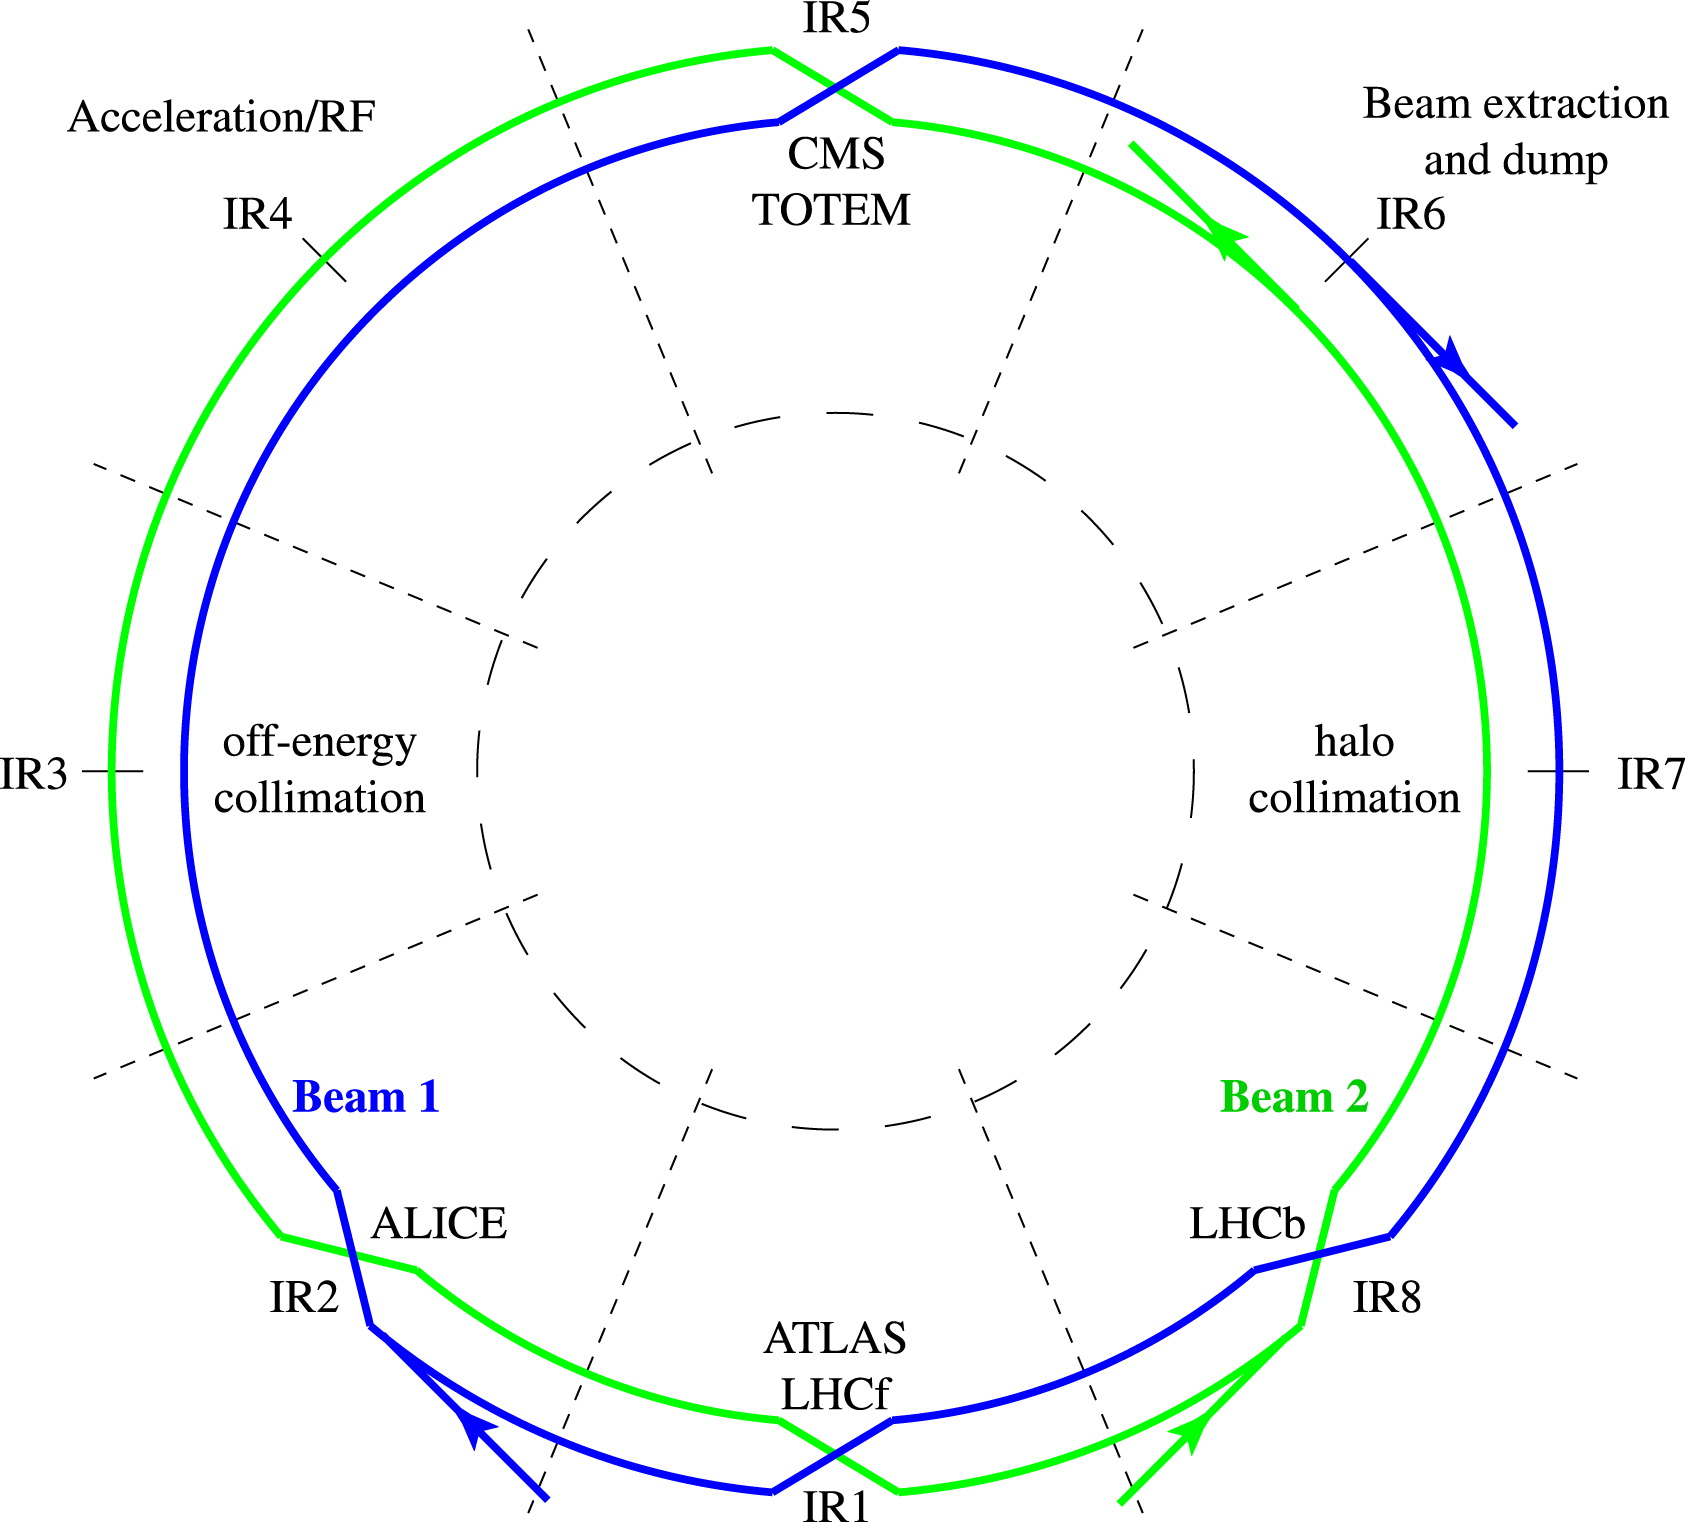
\includegraphics[width= 0.6\textwidth]{Figures/Chapter3/LHC_BasicLayout.jpg}
\caption[Basic schematic layout of the Large Hadron Collider]{Basic schematic layout of the LHC consisting of 8 arc sections along with the two circulating beams. The locations of the ATLAS, ALICE, CMS, and LHCb experiments are also displayed. Figure taken from Ref.~\cite{LHC_BasicLayout}.}
\label{Figure:Chapter3_LHC_BasicLayout}
\end{figure}

\newpage
Before entering the LHC ring, protons are ramped up through a series of pre-accelerator stages. The LHC represents the final link in this injector chain~\cite{LHC_InjectorComplex}, as shown in Fig.~\ref{Figure:Chapter3_LHC_Complex}. The first step is the \textbf{\ac{LINAC4}}~\cite{LINAC4}, where hydrogen gas is ionised to produce negative hydrogen ions and accelerated to $160\MeV$ for injection into the \textbf{\ac{PSB}}. During injection into the PSB, electrons are stripped off, leaving a pure proton beam that the PSB then accelerates to $2.0\GeV$. From there, the beam enters the \textbf{\ac{PS}}, raising its energy to $26\GeV$, before moving on to the \textbf{\ac{SPS}}, which boosts it to $450\GeV$. The beam is then injected into the LHC, where its energy is ramped up to several $\TeV$ in less than half an hour.

\begin{figure}[h]
\centering
\includegraphics[width= 0.85\textwidth]{Figures/Chapter3/LHC_AcceleratorComplex.pdf}
\caption[Schematic diagram of the CERN accelerator complex]{Schematic diagram of the CERN accelerator complex. Figure taken from Ref.~\cite{LHC_InjectorComplex}.}
\label{Figure:Chapter3_LHC_Complex}
\end{figure}

The \textbf{LHC} \textit{functions as a synchrotron accelerator}: protons continuously circulate the ring while radio-frequency (RF) cavities incrementally boost their energy. The strength of the bending magnets increases in synchrony with the rising beam momentum, allowing the particles to remain on a fixed trajectory. A network of 1,232 superconducting niobium-titanium dipole magnets, cooled to $1.9\unit{K}$ with superfluid helium, generates magnetic fields of up to $8.4\unit{T}$ to guide the beams along their circular path. At each of the four principal collision points, inner triplet quadrupole magnets compress the beams to reduce their transverse size, effectively squeezing them to maximise collision rates. These specifications reflect the accelerator complex's capabilities following upgrades completed during the most recent long shutdown.

\subsection{Cross section and Luminosity}

\textit{Cross section} and \textit{luminosity} are essential for predicting collision rates in the detector. The cross-section $\sigma(\sqrt{s})$ describes the probability of a given process occurring at centre-of-mass energy $\sqrt{s}$. However, knowing how often collisions occur also depends on how many particles are available to interact, which is described by the \textit{instantaneous luminosity} ($\mathscr{L}$). This quantity measures the number of particles passing through a unit area per unit time at the interaction point and depends on the detailed structure of the beams.

Since the proton beams at the LHC are not continuous streams but are composed of discrete bunches, the temporal structure of the beams directly impacts the collision frequency. Each bunch contains roughly $1.1\times10^{11}$ protons. During Run 2, the beams carried up to 2,220 bunches in 2016 and 2,556 bunches in 2017-2018. In 2022–2023, this number increased to a maximum of 2,808 bunches per beam, with bunches spaced by $25\unit{ns}$, corresponding to a crossing rate of $40\unit{MHz}$. The number of bunches, the number of protons per bunch, and the bunch spacing together determine the beam intensity and collision frequency, and therefore contribute directly to the luminosity. The dependence of the instantaneous luminosity on the beam parameters can be expressed as:

\begin{equation_pad}
\begin{aligned}
    \mathscr{L} &= \gamma \frac{n_b N^2 f_{\text{rev}}}{4\pi \beta^* \epsilon_n} R \\
    R &= 1 / \sqrt{1 + \left( \frac{\theta_c \sigma_z}{2\sigma} \right) }
\end{aligned}
\end{equation_pad}

where $\gamma$ is the proton beam energy expressed in rest mass units, $n_b$ is the number of bunches per beam, $N$ is the number of particles per bunch, $f_{rev}$ is the revolution frequency, $\beta^*$ is the beam beta function at the collision point and $\epsilon_n$ is the normalised transverse beam emittance. The term R is a geometrical reduction factor for luminosity. This is expressed as a function of the crossing angle of the beams at the collision point ($\theta_c$) and the transverse(longitudinal) spread of the particle bunch, $\sigma_z(\sigma)$. 

Because the beam parameters evolve over time, the luminosity is not constant. Therefore, the more appropriate quantity is the \textit{integrated luminosity} ($\mathscr{L}_{int}$), which represents the total data collected over a given period:

\begin{equation_pad}
    \mathscr{L}_{int} = \int \mathscr{L}(t) dt
\end{equation_pad}

The total number of events $(\mathscr{N})$ for a particular process with cross-section $\sigma$ over a fixed period can then be expressed as:

\begin{equation_pad}
    \mathscr{N} = \sigma \cdot \mathscr{L}_{int}
\end{equation_pad}

A summary of the total integrated luminosity delivered to the CMS experiment since 2015 is provided in Fig.~\ref{Figure:Chapter3_CMS_IntegratedLumi}.

\begin{figure}[h]
\centering
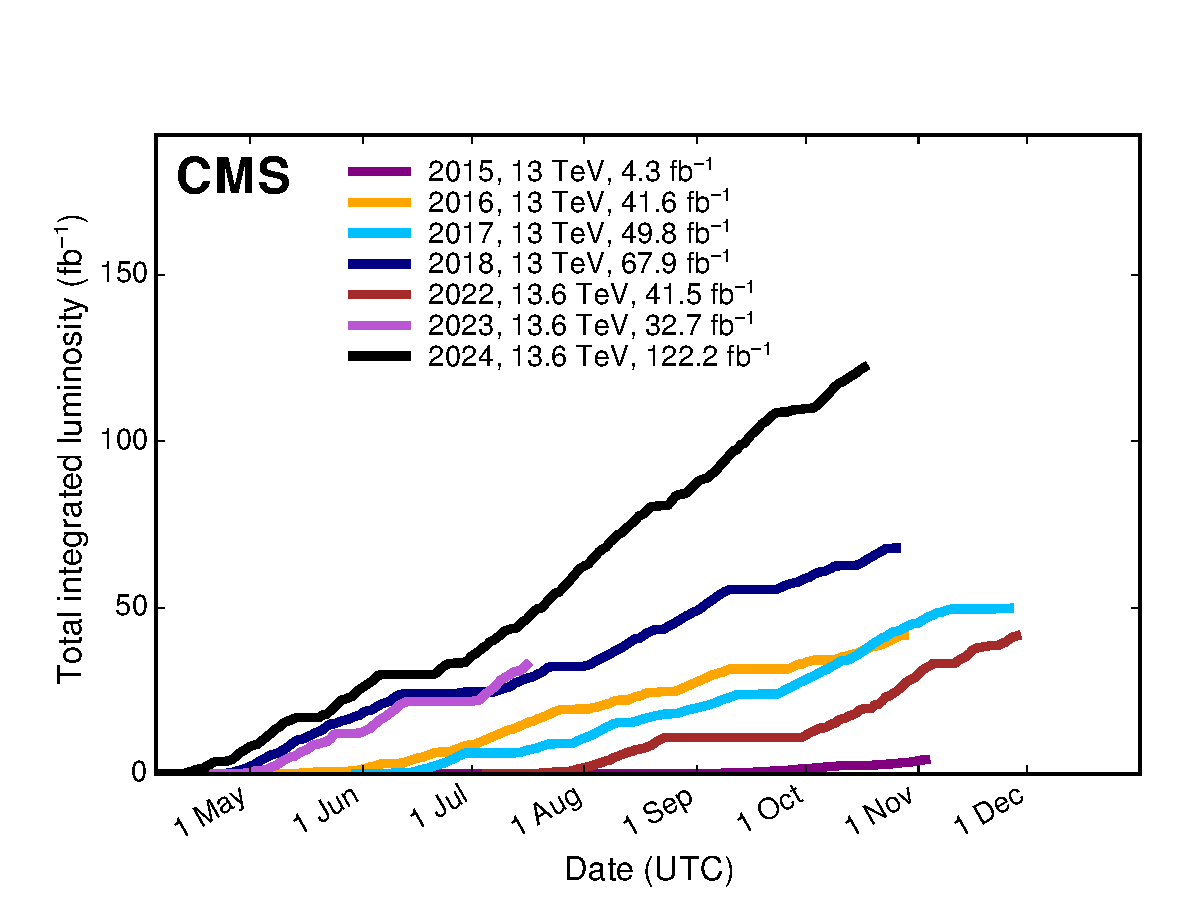
\includegraphics[width= 0.7\textwidth]{Figures/Chapter3/CMS_IntegratedLumi.pdf}
\caption[Total integrated luminosity delivered to the CMS experiment between 2015 and 2024]{Total integrated luminosity delivered to the CMS experiment between 2015 and 2024. Data collected from all periods except 2015 and 2024 are used in this thesis. Figure taken from Ref.~\cite{CMS_IntegratedLumi}.}
\label{Figure:Chapter3_CMS_IntegratedLumi}
\end{figure}

\subsection{Pileup}

To maximise the probability of observing rare processes, the LHC collides large bunches of protons, resulting in high instantaneous luminosity. However, this also introduces challenges: \textit{when bunches collide, multiple protons interact simultaneously, and the vast majority of these pp collisions do not involve a hard scattering process}. This means that for each event, the pp interaction of interest is recorded along with additional pp interactions, called \textbf{\ac{PU}} interactions. 

These PU interactions act as background noise, complicating the reconstruction of the primary hard-scattering event and degrading the performance of many physics measurements. As instantaneous luminosity increases, PU becomes more severe, and removing the unwanted overlap collisions requires increasingly sophisticated mitigation techniques. Figure~\ref{Figure:Chapter3_CMS_Pileup} displays the PU conditions encountered by the CMS experiment between 2015 and 2024.

\begin{figure}[h]
\centering
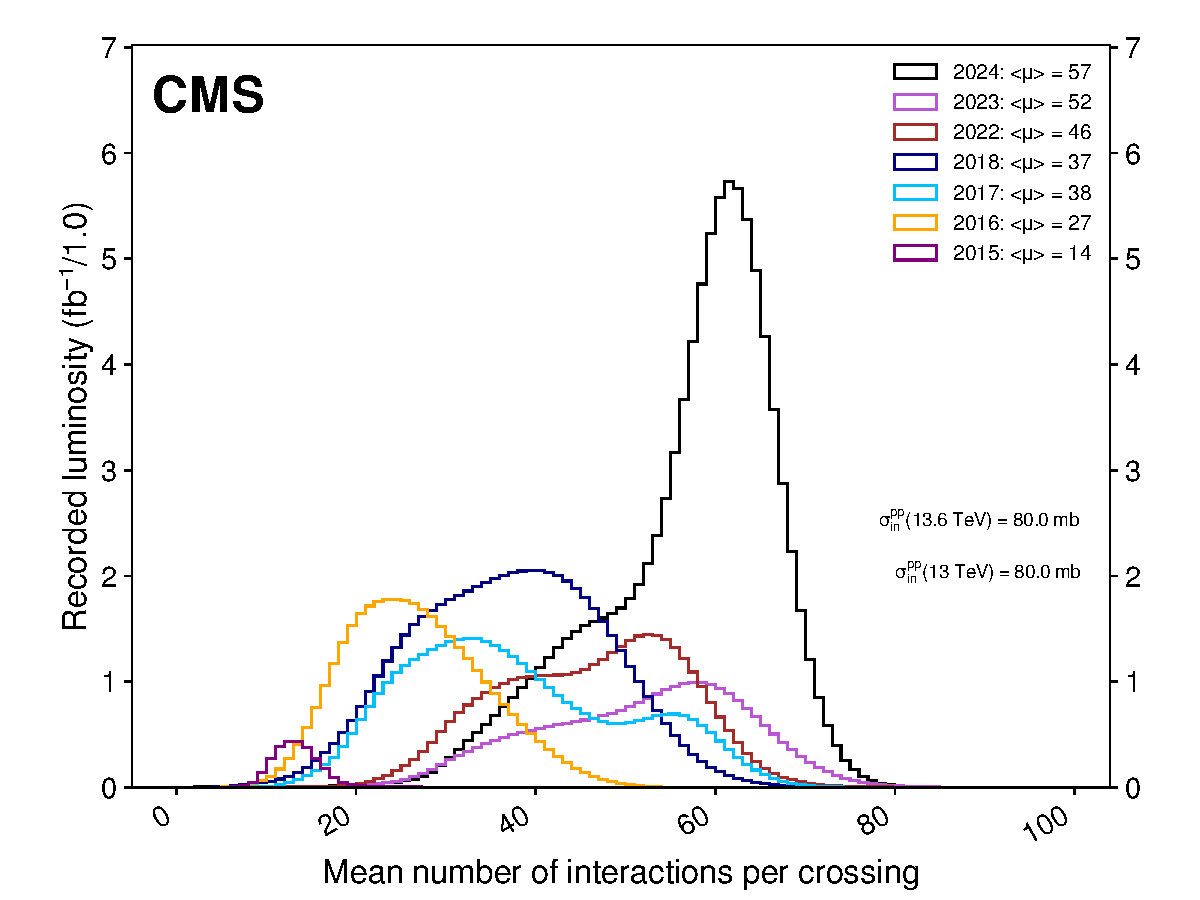
\includegraphics[width= 0.7\textwidth]{Figures/Chapter3/CMS_Pileup.pdf}
\caption[Distribution of the average number of interactions per bunch crossing for pp collisions at CMS between 2015 and 2024]{Distribution of the average number of interactions per bunch crossing for pp collisions between 2015 and 2024, using data from the CMS experiment. Figure taken from Ref.~\cite{CMS_IntegratedLumi}.}
\label{Figure:Chapter3_CMS_Pileup}
\end{figure}

\section{The CMS Detector}
\label{Section:Chapter3_CMS_Detector_Introduction}
CMS is one of the two general-purpose detectors at the LHC, built to explore a wide range of high-energy physics phenomena. The design of the CMS detector was shaped by the ambitious goals of the LHC physics programme~\cite{LHC_CMS}, which demanded precise and efficient measurements under challenging experimental conditions. To accomplish these objectives, several key performance requirements were identified:

\begin{itemize}
  \item Identification \& precise momentum reconstruction of muons over a broad range of momenta and angles; dimuon mass resolution $\sim1\%$ at $100\GeV$; unambiguous muon charge identification up to $1\TeV$
  \item High momentum resolution \& reconstruction efficiency for charged particles; efficient $\tau$‐lepton and b‐jet identification
  \item Photon/electron energy measurement with excellent resolution; diphoton and dimuon mass resolution $\sim1\%$ at $100\GeV$ over a wide geometrical coverage
  \item Effective $\pi^0$ rejection; efficient isolation of photons and leptons in high‐luminosity, high‐occupancy conditions
  \item Precise dijet mass reconstruction and MET resolution
\end{itemize}

CMS employs a compact, layered detector system arranged cylindrically around the interaction point to fulfil these performance requirements, providing nearly 4$\pi$ solid-angle coverage. The entire detector is $21.6\unit{m}$ long and has a diameter of $14.6\unit{m}$ while weighing $12,500\unit{t}$. This makes CMS one of the largest yet compact detectors ever engineered for a particle physics experiment. Closest to the beam pipe lies the \textbf{silicon tracker}, which precisely tracks charged particles. It is surrounded by the \textbf{\ac{ECAL}}, optimised for measuring the energy of electrons and photons with high precision. The \textbf{\ac{HCAL}} follows and is responsible for absorbing and measuring the energy of hadrons. These three subdetectors are enclosed within a powerful $13\unit{m}$ long, $6\unit{m}$ inner-diameter, $3.8\unit{T}$ \textbf{superconducting solenoid}. Embedded within the iron return yoke of the solenoid is the \textbf{muon detection system}. A schematic of the full CMS detector is shown in Fig.~\ref{Figure:Chapter3_CMS_schematic}, providing an overview of its cylindrical geometry and layered structure around the LHC interaction point. The following sections will provide a more detailed discussion of each of the major subdetector systems introduced here. A complementary longitudinal slice through the detector is shown in Fig.~\ref{Figure:Chapter3_CMS_slice}, serving as a visual reference for the detailed subdetector descriptions that follow.

\begin{figure}[h]
\centering
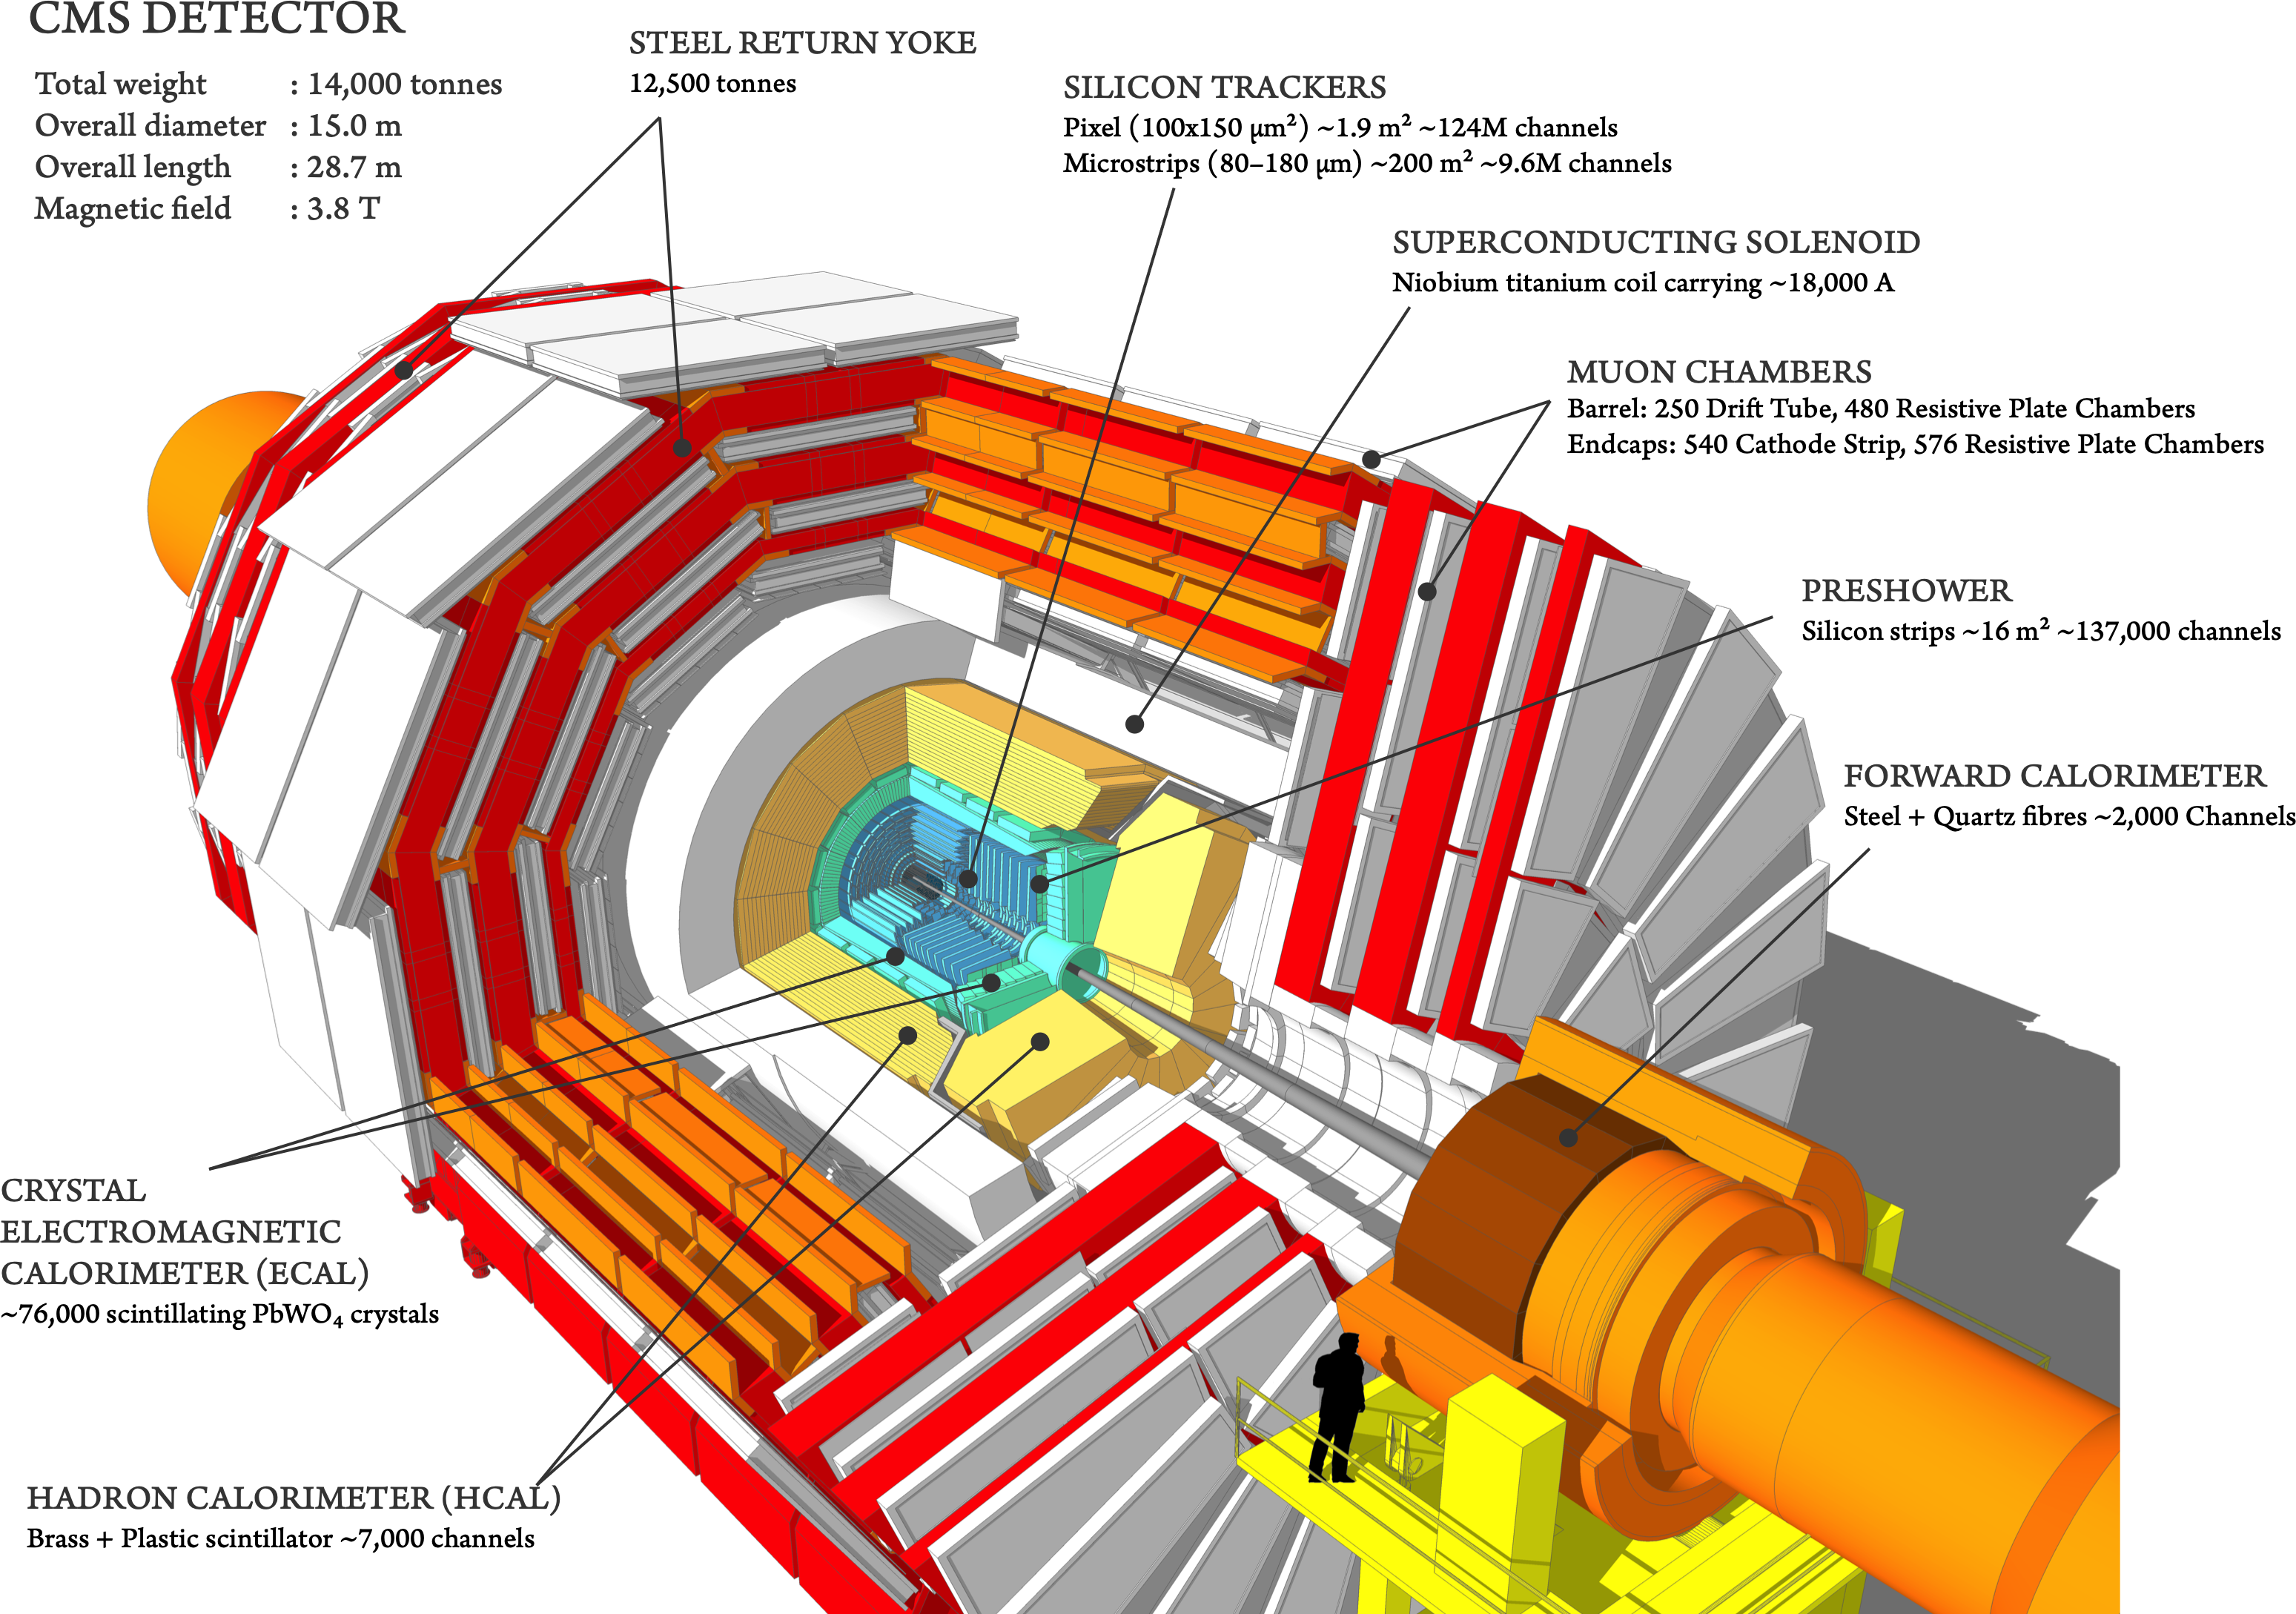
\includegraphics[width= 0.8\textwidth]{Figures/Chapter3/CMS_Detector.pdf}
\caption[Schematic drawing of the CMS detector]{Schematic drawing of the CMS detector. Figure taken from Ref.~\cite{CMS_Detector_Run3}.}
\label{Figure:Chapter3_CMS_schematic}
\end{figure}

\begin{figure}[h]
\centering
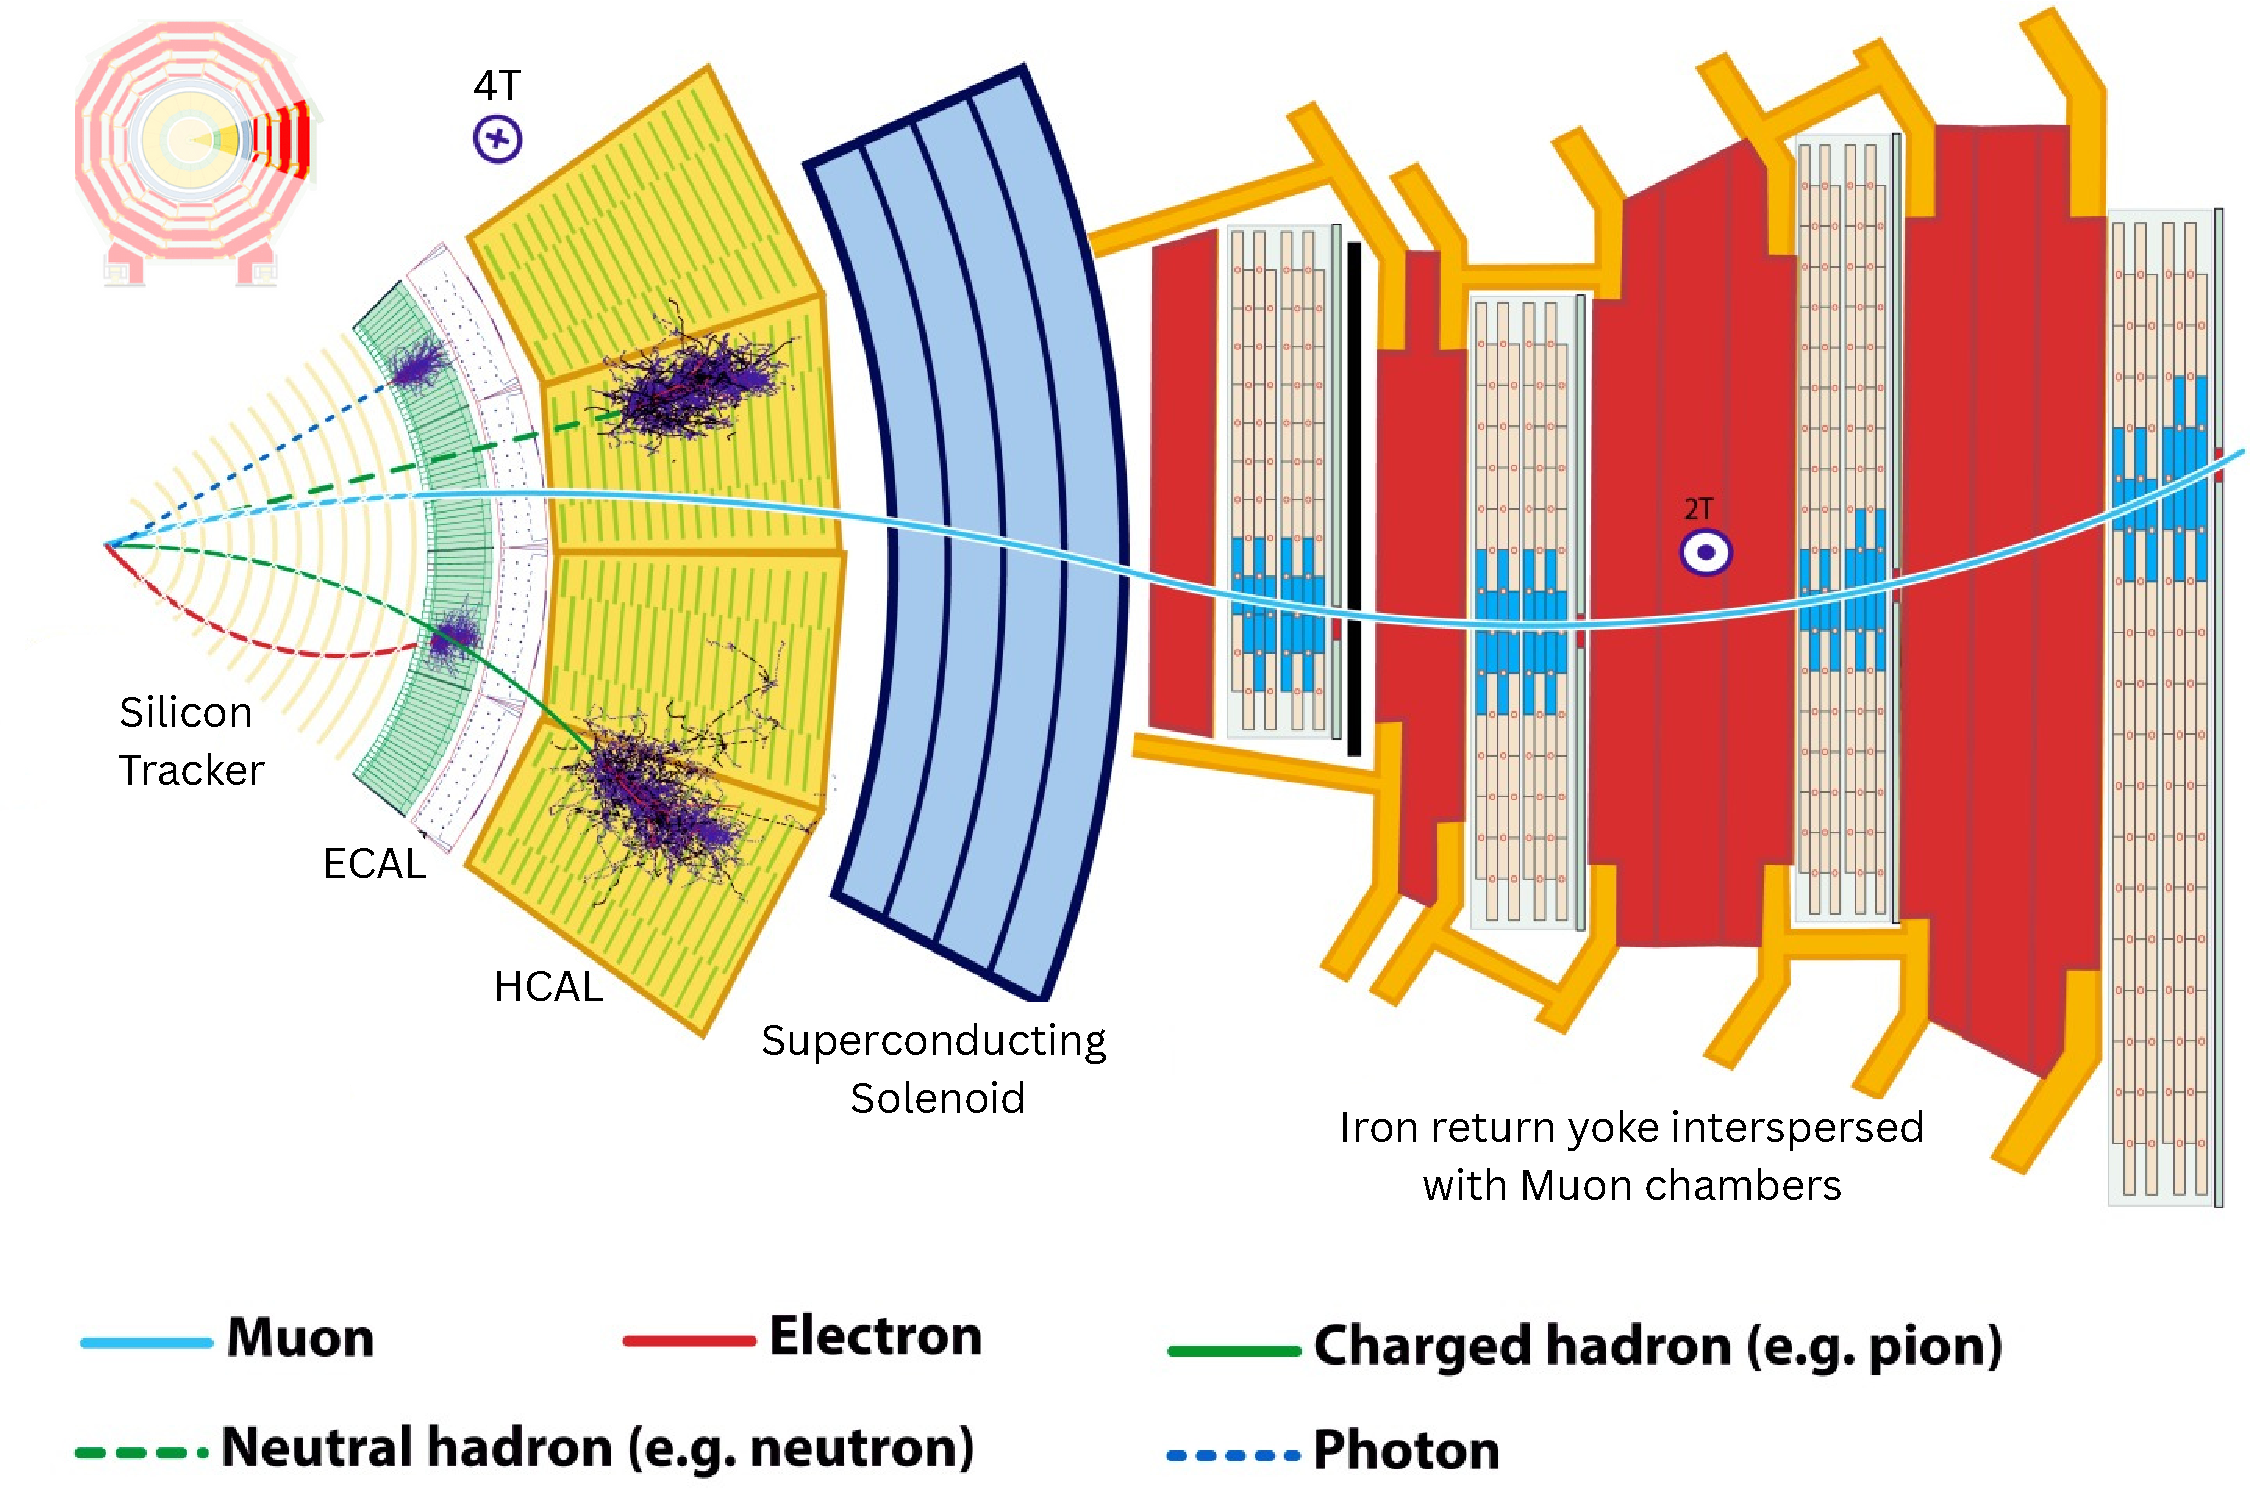
\includegraphics[width= 0.8\textwidth]{Figures/Chapter3/CMS_Detector_Slice.pdf}
\caption[Transverse slice of the CMS detector]{A transverse slice of the CMS detector displaying the individual subsystems and their response to different types of particles. Figure adjusted from Ref.~\cite{CMS_Detector_Slice}.}
\label{Figure:Chapter3_CMS_slice}
\end{figure}

\clearpage
\subsection{Co-ordinate system}
CMS adopts a right-handed Cartesian coordinate system centred at the nominal collision point. The $x$-axis points towards the centre of the LHC ring, and the $y$-axis points vertically upwards, while the $z$-axis points along the beam direction towards the Jura mountains, as illustrated in Fig.~\ref{Figure:Chapter3_CMS_CoordinateSystem}.

\begin{figure}[h]
\centering
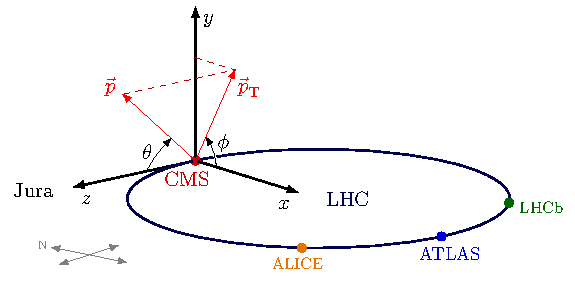
\includegraphics[width= 0.8\textwidth]{Figures/Chapter3/CMS_CoordinateSystem.pdf}
\caption{The CMS detector coordinate system.}
\label{Figure:Chapter3_CMS_CoordinateSystem}
\end{figure}

In this system, the plane perpendicular to the beam axis, $x-y$ plane, is referred to as the \textit{transverse plane}, while the $z$-axis defines the \textit{longitudinal direction}. The \textit{azimuthal angle} $\phi \in [0,2\pi]$ is the angle with respect to the positive $x$-axis in the transverse plane, while the \textit{polar angle} $\theta \in [0,\pi]$ is with respect to the $z$-axis. Rather than using $\theta$ directly, it is common in collider physics to introduce \textit{pseudorapidity} ($\eta$), defined as

\begin{equation_pad}
    \eta = - \ln\left[\tan(\theta/2)\right]
\end{equation_pad}

A key property of this quantity is that the difference in pseudorapidity ($\Delta\eta$) between two vectors is invariant under Lorentz boosts along the longitudinal $z$-axis. This is convenient in hadron collider experiments, where the parton-parton centre-of-mass frame is often significantly boosted along the beam direction due to the variable momentum fractions carried by the incoming partons. Additionally, $\eta$ provides a nearly linear mapping of $\theta$ (shown in Fig.~\ref{Figure:Chapter3_Pseudorapidity}), facilitating a simple description of particle emission angles relative to the beam axis. This property allows for a natural segmentation of the detector into barrel and endcap regions based on $\eta$.

\begin{itemize} 
\item \textbf{Barrel region}: The central cylindrical region of the detector, located closest to the primary interaction point and optimised for particles emitted at large angles to the beamline ($\ie$ low $|\eta|$). 
\item \textbf{Endcap regions}: Located at either end of the barrel along the $z$-axis, designed to detect particles emitted at small angles with respect to the beamline ($\ie$ high $|\eta|$). 
\end{itemize}

\begin{figure}[h]
\centering
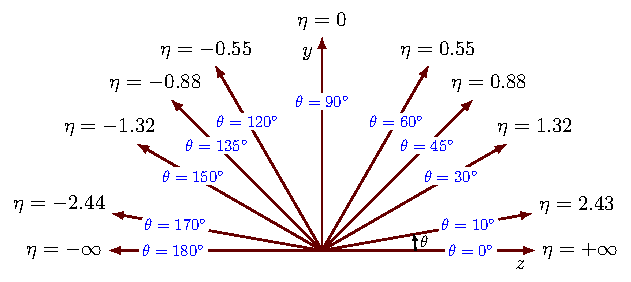
\includegraphics[width= 0.8\textwidth]{Figures/Chapter3/Pseudorapidity.pdf}
\caption{Illustration of the relationship between pseudorapidity ($\eta$) and polar angle ($\theta$).}
\label{Figure:Chapter3_Pseudorapidity}
\end{figure}

At the LHC, the initial momentum component of the system perpendicular to the beam axis is nearly zero because of the head-on nature of the beam. This kinematic quantity is referred to as the transverse momentum ($p_\mathrm{T}$) and is defined as:

\begin{equation_pad}
    p_\mathrm{T} = \sqrt{p_x^2 + p_y^2}
\end{equation_pad}

Transverse momentum is a central observable in collider physics. It provides a direct probe of hard interaction processes characterised by large momentum transfers. A complementary quantity to the transverse momentum is the missing transverse momentum ($E_\mathrm{T}^{\text{miss}}$), which is defined as the negative vector sum of the transverse momenta of all reconstructed particles in an event. This is a critical quantity serving as an estimator of the transverse momentum carried by non-interacting or undetected particles.

The radial distance from the beam axis is typically expressed as $r = \sqrt{x^2+y^2}$. Additionally, it is also convenient to express the distance metric ($\Delta R$) between two objects in a Lorentz-invariant way as:

\begin{equation_pad}
    \Delta R = \sqrt{(\Delta\eta)^2 + (\Delta \phi)^2}
\end{equation_pad}

This quantity is important in object reconstruction, as discussed in Section~\ref{Section:Chapter4}.%

\subsection{Magnet System}

As its name implies, CMS is defined by its central feature: the solenoid magnet. This critical component generates a very strong magnetic field that bends the trajectories of charged particles as they traverse the detector. This enables precise measurements of their momenta and electric charges. 

The \textbf{solenoid} spans $13\unit{m}$ in length and $6\unit{m}$ in diameter, capable of producing a magnetic field of up to $4\unit{T}$, but is currently operated at $3.8\unit{T}$ for enhanced long-term stability. The strong field ensures that low-momentum charged particles are sufficiently curved, confining them within the inner tracking system and aiding in precise momentum resolution. This not only improves tracking quality but also helps mitigate calorimeter noise by preventing soft particles from reaching the calorimeters.

Outside the solenoid, the muon detection system is embedded within segmented layers of iron, forming the \textbf{iron yoke}. This massive structure, weighing approximately $10,000\unit{t}$, serves two primary purposes: it returns about two-thirds of the magnetic flux generated inside the detector and provides structural support for the muon chambers. By returning the flux, the iron yoke significantly reduces the magnetic field outside the detector. This magnetic field configuration causes a ``\textit{double bending}'' of muon trajectories: first in one direction as muons pass through the inner silicon tracker, and then in the opposite direction as they traverse the muon chambers embedded in the iron yoke. This double bending significantly enhances the overall muon momentum resolution.

\subsection{Inner tracking system}
The CMS interaction point is surrounded by the innermost subdetector, the \textbf{silicon tracker}, which measures $5.8\unit{m}$ in length and $2.5\unit{m}$ in diameter~\cite{LHC_CMS,CMS_Detector_Run3}. The tracker plays a central role in reconstructing the trajectories of charged particles and in identifying both primary and secondary interaction vertices with high spatial precision.

At the LHC’s design luminosity, on the order of $10^3$ charged particles traverse the tracker volume per each $25\unit{ns}$ bunch crossing. To cope with the extreme occupancy, the tracker must combine high granularity with rapid signal readout. Furthermore, its proximity to the interaction point exposes it to a harsh radiation environment, necessitating the use of radiation-hard sensor technologies to preserve long-term performance.

To meet these demanding requirements, the CMS tracker employs \textit{silicon-based sensors}. However, these silicon sensors also require dedicated readout electronics and active cooling systems. These components contribute to the non-active material within the tracking volume, which must be carefully controlled. Excessive material leads to increased multiple scattering and energy loss, degrading momentum resolution and negatively impacting the performance of outer subdetectors such as the calorimeters.

As shown in Fig.~\ref{Figure:Chapter3_Tracker_MaterialBudget}, the material budget of the tracker is kept as low as possible, particularly in the central (low-$\eta$) region of the pixel detector, where precision tracking is most critical.

\begin{figure}[h]
    \centering
    % First row
    \begin{subfigure}[b]{0.49\textwidth}
        \centering
        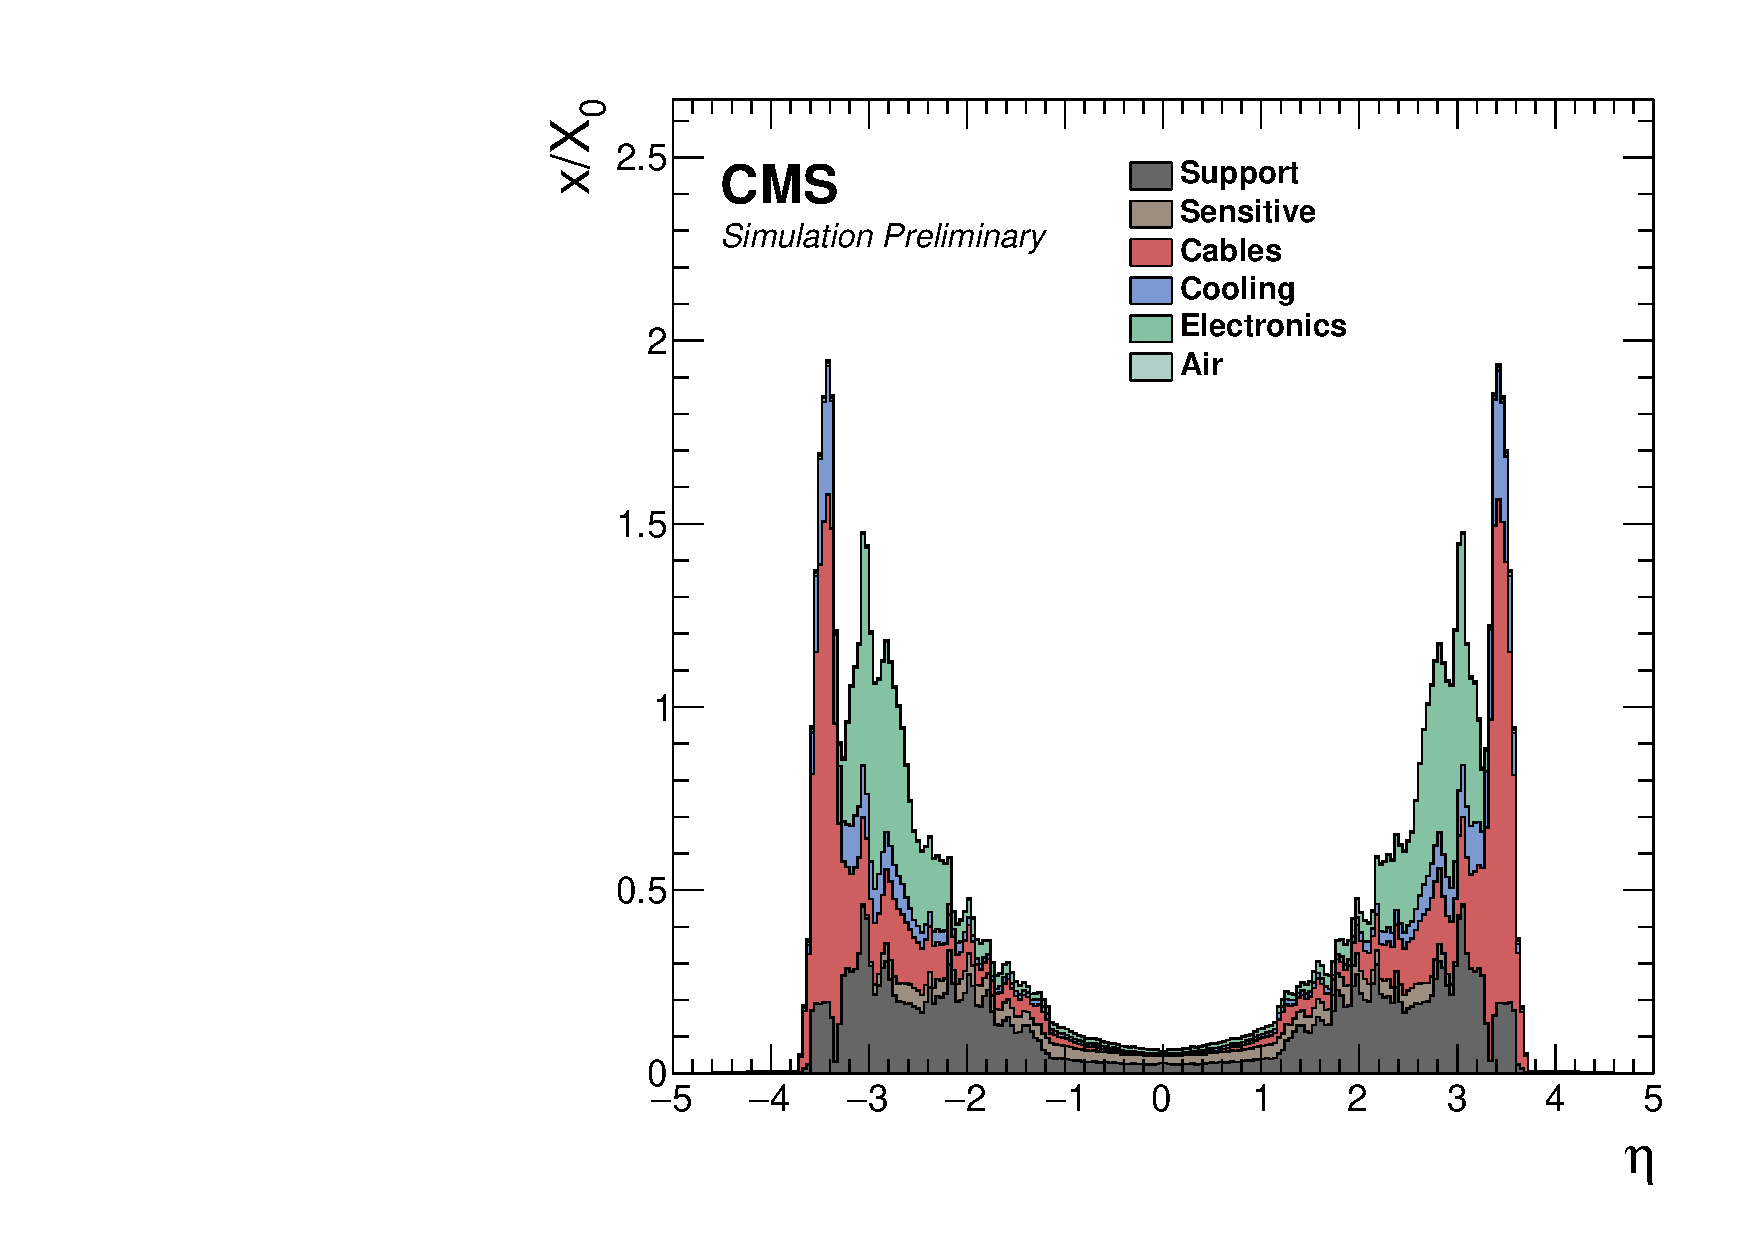
\includegraphics[width=\textwidth]{Figures/Chapter3/Material_Budget1.pdf}
        \caption{}
    \end{subfigure}
    \begin{subfigure}[b]{0.49\textwidth}
        \centering
        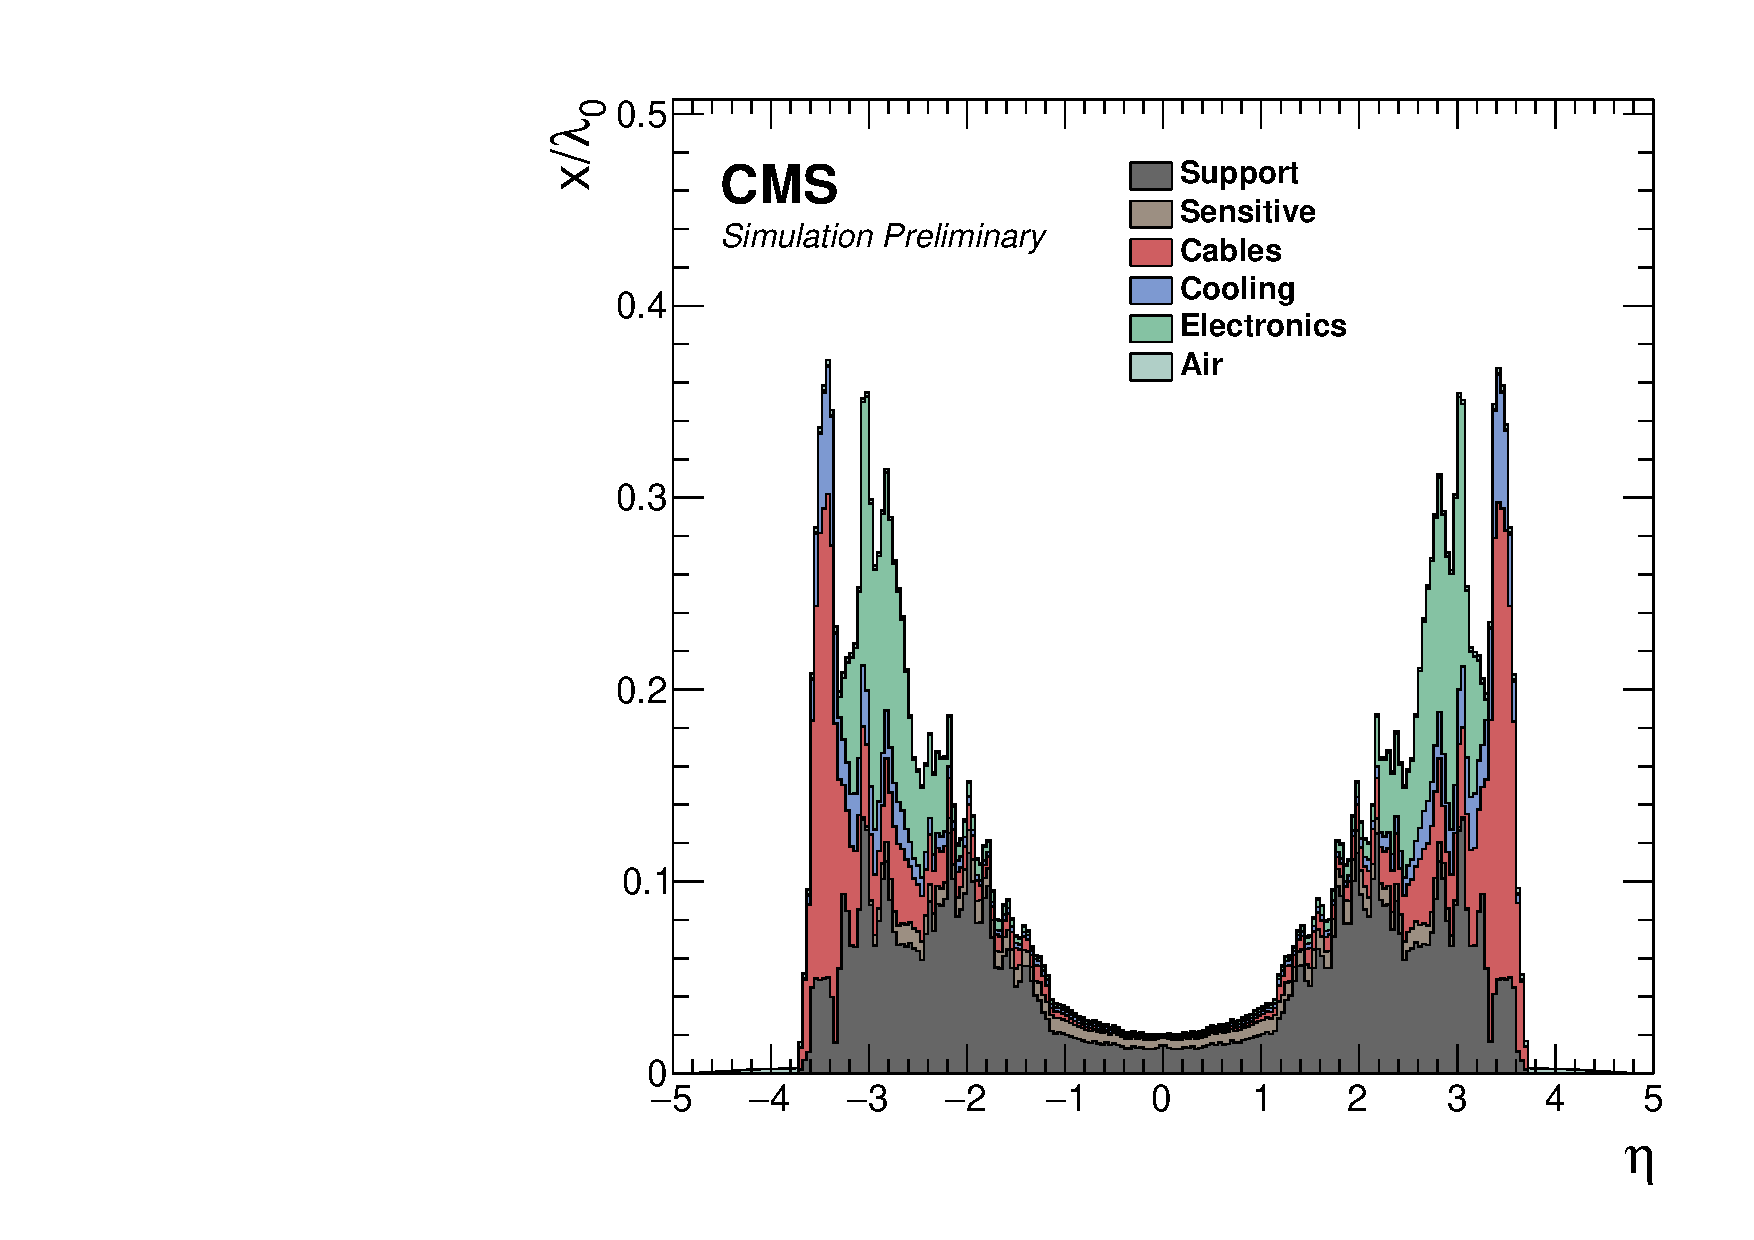
\includegraphics[width=\textwidth]{Figures/Chapter3/Material_Budget2.pdf}
        \caption{}
    \end{subfigure}
\caption[Simulation of the CMS pixel detector material budget]{Simulation of the CMS pixel detector material budget as a function of $\eta$ in units of ($\textbf{a}$) radiation length and ($\textbf{b}$) hadronic interaction length for different detector components. Figure taken from Ref.~\cite{TrackerMaterialBudget_Pixel}.}
\label{Figure:Chapter3_Tracker_MaterialBudget}
\end{figure}

\newpage
\subsubsection{Pixel Detector}

The innermost component of the CMS tracking system is the \textbf{silicon pixel detector}. The original pixel detector~\cite{LHC_CMS}, installed in 2008, was designed to operate for up to ten years under the LHC’s nominal instantaneous luminosity of $1 \times 10^{34}\unit{cm}^{-2}\unit{s}^{-1}$, with the capacity to handle up to 25 PU interactions ber bunch crossing. However, even during Run-1, the LHC exceeded its design luminosity, exposing the pixel detector to increased radiation levels and causing rising readout inefficiencies. To maintain high tracking efficiency under upgraded luminosity conditions of up to $2 \times 10^{34}~\unit{cm}^{-2}\unit{s}^{-1}$ and PU levels of 50 or more, the CMS pixel detector underwent a major upgrade in 2017, referred to as the Phase-1 upgrade~\cite{CMS_Detector_Run3, CMS_Tracker_Phase1_Upgrade}. This upgrade introduced a more granular and radiation-tolerant detector layout, featuring four barrel layers and three endcap disks.

The \textbf{\ac{BPIX}} detector consists of four concentric cylindrical layers (L1-L4) positioned at radii of 29, 68, 109, and 160$\unit{mm}$ from the beamline. A total of 1,184 sensor modules are deployed in the barrel region. Each module contains a silicon sensor segmented into $160 \times 416$ individual pixels with a pitch of $100 \times 150\unit{\mu m}^2$, enabling high-resolution hit detection. Compared to the original pixel detector, the innermost layer (L1) was also moved closer to the interaction point by reducing the CMS beam pipe radius from 30 to 23$\unit{mm}$ in 2014. 

The \textbf{\ac{FPIX}} detector complements the barrel coverage by extending tracking capabilities in the forward region. It comprises three endcap disks on each side of the detector, located at distances of 291, 396, and 516$\unit{mm}$ from the interaction point. The forward region is equipped with 672 pixel modules, featuring the same fine segmentation and pixel pitch as the barrel modules. Together, the BPIX and FPIX systems provide approximately 124 million readout channels, ensuring precise tracking throughout the detector’s angular coverage.

The Phase-1 upgrade of the CMS pixel detector introduced significant improvements in geometry and coverage, as illustrated in Fig.~\ref{Figure:Chapter3_Pixel_Upgrade}. Additionally, substantial gains were also achieved in spatial resolution and tracking performance. The position resolution reaches approximately $11\unit{\mu m}$ in the $r-\phi$ direction and $24\unit{\mu m}$ in the $z$ direction for BPIX L3. Somewhat worse resolutions are observed in the innermost barrel layers due to higher radiation damage. For FPIX, the corresponding resolutions are about $12\unit{\mu m}$ ($r$) and $21\unit{\mu m}$ ($z$). 

\begin{figure}[h]
\centering
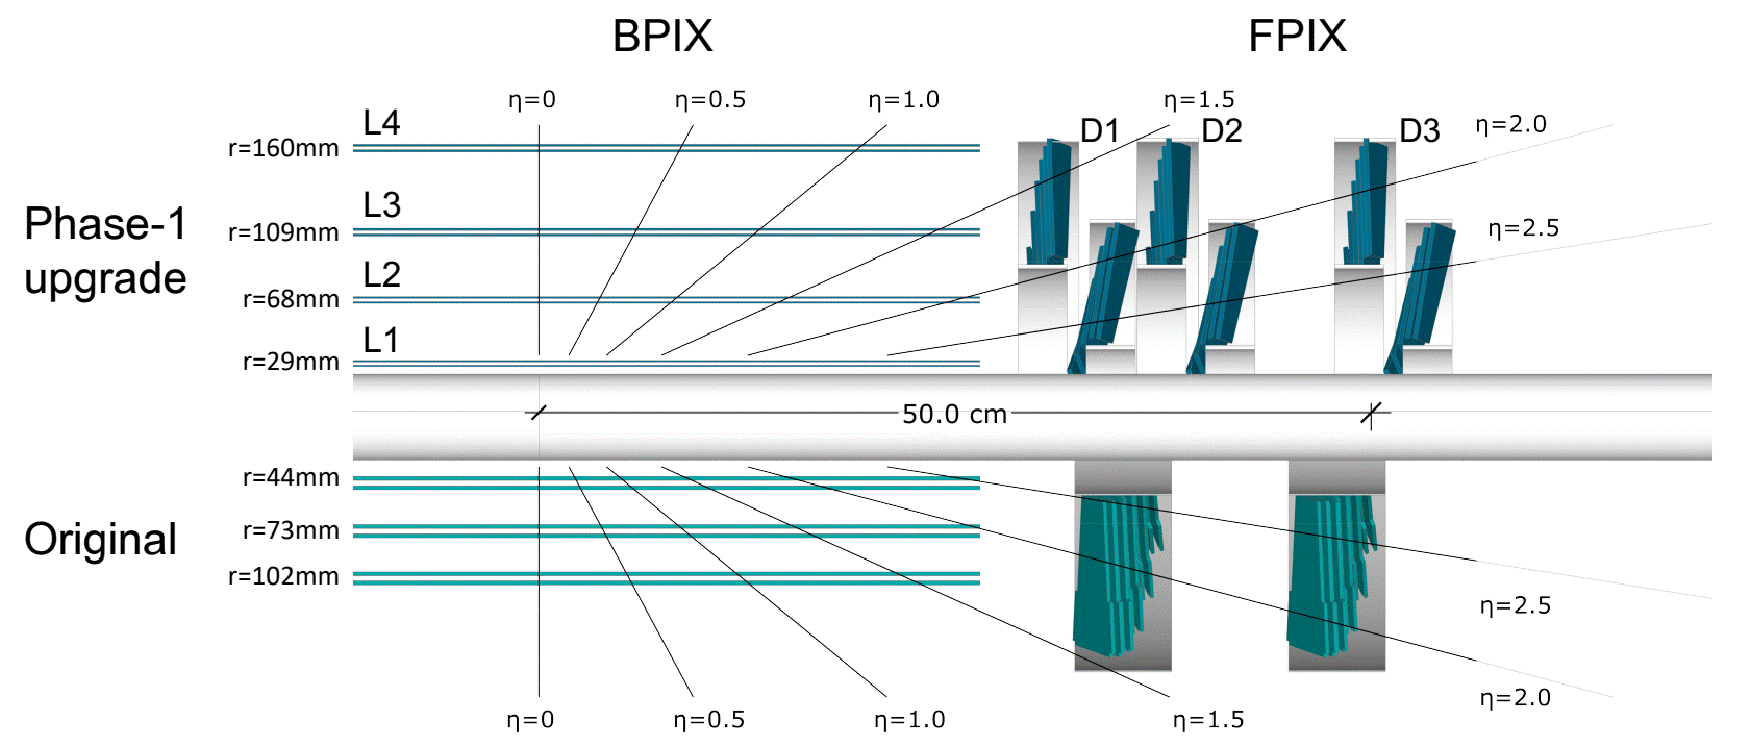
\includegraphics[width=1\textwidth]{Figures/Chapter3/CMS_Pixel_Upgrade.pdf}
\caption[Longitudinal view of CMS pixel detector before and after Phase-1 Upgrade]{Longitudinal view of CMS pixel detector comparing its structure before (lower part) and after (upper part) the Phase-1 Upgrade. Figure taken from Ref.~\cite{CMS_Detector_Run3}.}
\label{Figure:Chapter3_Pixel_Upgrade}
\end{figure}

The improved granularity and four-hit coverage introduced in the Phase-1 pixel detector enable robust three-dimensional reconstruction of charged particle trajectories, which is essential for precise identification of both primary and secondary vertices. Consequently, these tracking enhancements lead to improved vertex reconstruction performance. As shown in Fig.~\ref{Figure:Chapter3_Pixel_Vertex_Resolution}, the transverse ($x,y$) vertex resolution achieved with the Phase-1 detector is significantly better than that of the Phase-0 detector.

\begin{figure}[h]
    \centering
    % First row
    \begin{subfigure}[b]{0.49\textwidth}
        \centering
        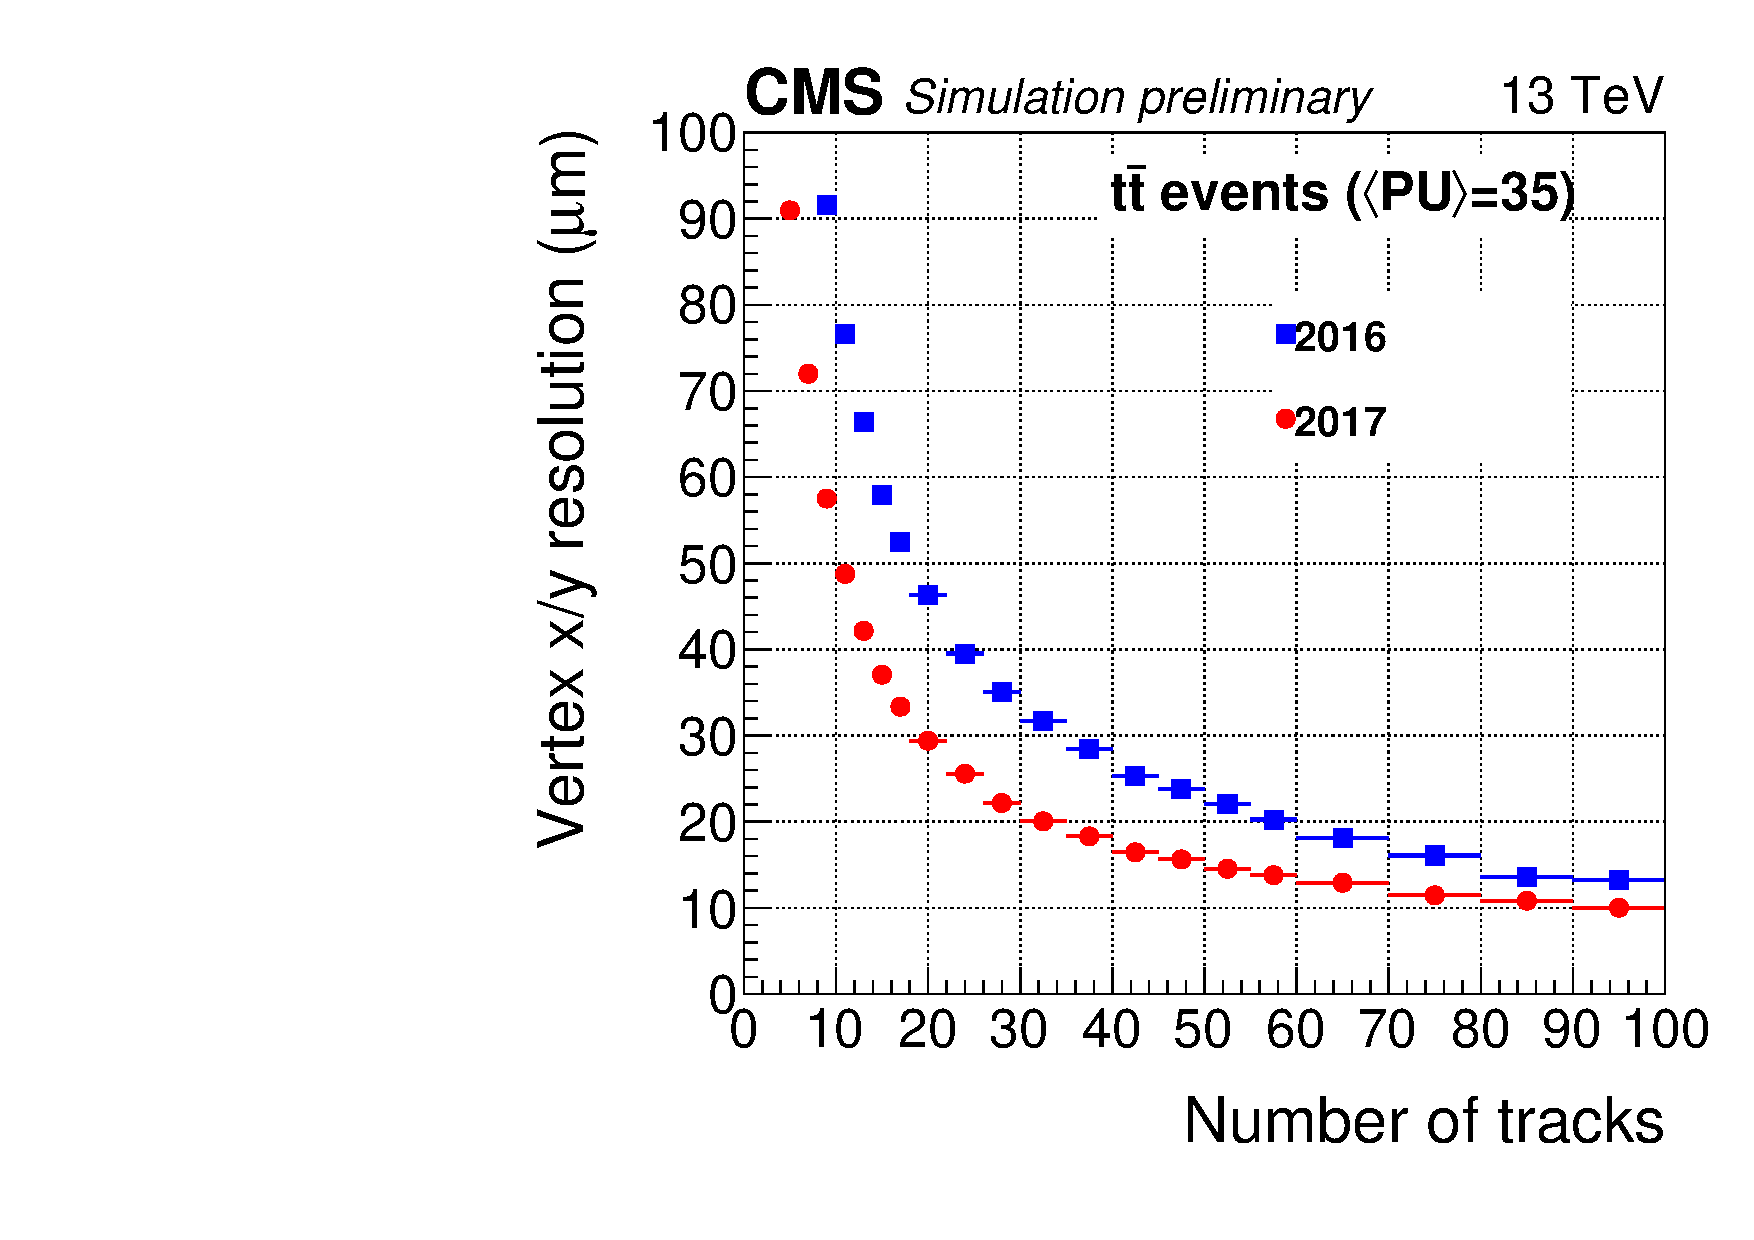
\includegraphics[width=\textwidth]{Figures/Chapter3/Pixel_Vertex_XY_Resolution.pdf}
        \caption{}
    \end{subfigure}
    \begin{subfigure}[b]{0.49\textwidth}
        \centering
        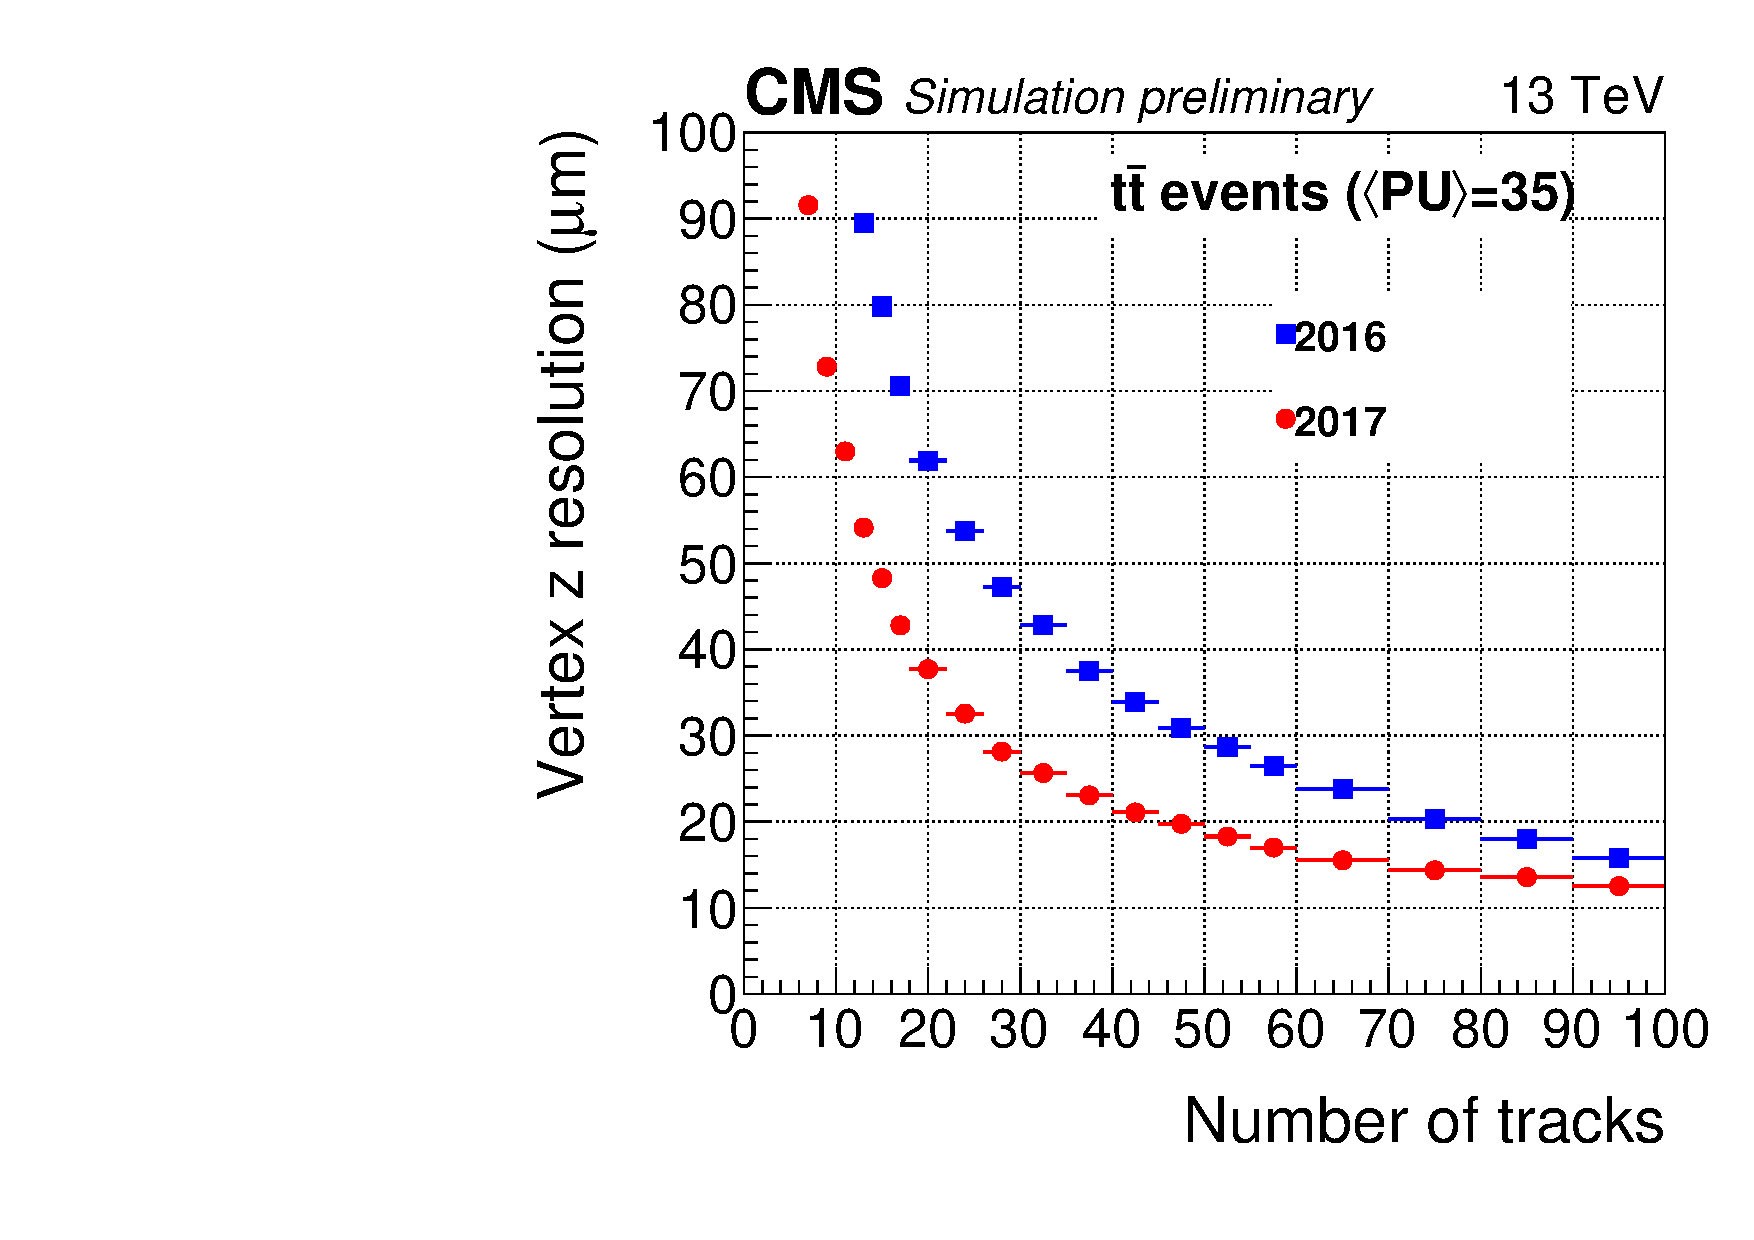
\includegraphics[width=\textwidth]{Figures/Chapter3/Pixel_Vertex_Z_Resolution.pdf}
        \caption{}
    \end{subfigure}
\caption[Vertex resolution comparison between Phase-0 and Phase-1 pixel detectors]{Comparison of the simulated CMS vertex resolution between the Phase-0 and Phase-1 pixel detectors as a function of the number of tracks used in the vertex fit. \textbf{(a)} Transverse ($x,y$) vertex resolution. \textbf{(b)} Longitudinal ($z$) vertex resolution. Figures taken from Ref.~\cite{Pixel_Vertex_Performance}.}

\label{Figure:Chapter3_Pixel_Vertex_Resolution}
\end{figure}


\subsubsection{Silicon Strip Tracker}
Surrounding the pixel detector is the \textbf{\ac{SST}}, illustrated in Fig.~\ref{Figure:Chapter3_Tracker_Geometry}. In the outer tracking region, lower particle occupancy allows the use of silicon strips instead of pixels, relaxing granularity requirements and enabling larger sensor elements. The SST covers an active area of approximately $198\unit{m}^2$ and contains 9.3 million silicon micro-strips distributed across 15,148 detector modules. It is composed of four main subsystems: the \ac{TIB}, \ac{TID}, \ac{TOB}, and \ac{TEC}.

\begin{figure}[h]
\centering
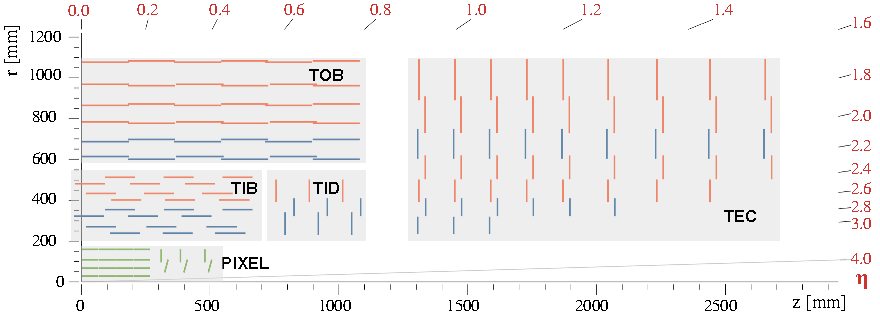
\includegraphics[width=1\textwidth]{Figures/Chapter3/Phase1_Tracker.pdf}
\caption[Schematic of CMS inner tracking system in the $(r-z)$ plane]{Schematic view of one-quarter of the CMS inner tracking system in the $(r-z)$ plane. The pixel detector is depicted in green, located close to the beamline. Single-sided and double-sided strip modules are depicted as red and blue segments, respectively. Figure adjusted from Ref.~\cite{CMS_Detector_Run3}.}
\label{Figure:Chapter3_Tracker_Geometry}
\end{figure}

The \textbf{TIB} is made up of four cylindrical barrel layers located just outside the pixel detector. It provides precise tracking in the central pseudorapidity region and extends out to a radius of $r < 550\unit{mm}$. To ensure complete coverage and continuity in tracking performance, the TIB is complemented by the \textbf{TID}, which consists of three disk-shaped structures at each end of the TIB, extending the longitudinal reach to $|z| < 1180\unit{mm}$. Together, the TIB and TID form the inner part of the strip tracking system, which is crucial for linking tracks from the pixel detector to the outer layers.

The \textbf{TOB} extends the radial coverage beyond the inner systems, occupying the region $r > 550\unit{mm}$. It consists of six cylindrical barrel layers, providing high-precision measurements over a larger area with longer strip modules. The TOB ensures efficient momentum resolution and track reconstruction for particles passing through the outer barrel region, especially those with lower transverse momentum.

The \textbf{TEC} completes the strip tracker by covering the forward pseudorapidity regions. Each TEC consists of nine disks positioned between $1240 < |z| < 2820\unit{mm}$ on either side of the detector. These disks contain up to seven concentric rings of silicon strip modules, which are carefully arranged to maintain uniform tracking performance and coverage up to $|\eta| \simeq 2.5$.

In the barrel sections, the modules are oriented to measure the radial $r\text{-}\phi$ coordinates. Conversely, in the TID and TEC sections, they are primarily aligned to measure $\phi\text{-}z$ coordinates.

In the innermost two layers of the TIB and TOB, the first two rings of the TID, and rings 1, 2, and 5 of the TEC, double-sided modules are deployed. These consist of two single-sided sensors mounted back-to-back with a stereo angle of $100\unit{mrad}$. The combination of their signals enables three-dimensional hit reconstruction, providing an additional measurement of the $z$ coordinate in the barrel and the $r$ coordinate in the disk regions.

\subsection{Electromagnetic calorimeter}

As outlined by the LHC physics requirements in Section~\ref{Section:Chapter3_CMS_Detector_Introduction}, precise reconstruction of electromagnetic particles and robust suppression of background processes ($\pi^0 \to \gamma \gamma$) are essential for CMS. The CMS \textbf{ECAL}~\cite{LHC_CMS,CMS_Detector_Run3,CMS_ECAL_Performance_Run2} is designed to meet these demands, providing high-resolution energy measurements for electrons and photons. It is composed of three main subsystems: a central barrel calorimeter, two endcap calorimeters, and a preshower detector situated in front of the endcaps.

The ECAL is a hermetic homogeneous calorimeter consisting of 61,200 lead tungstate (PbWO$_4$) crystals mounted in the central \textbf{barrel} part. These crystals are arranged in a quasi-projective geometry, with their axes slightly tilted ($3^\circ$) relative to the line from the nominal interaction point. This geometry minimises gaps in the detector and reduces the probability of particles passing through the cracks between crystals. The barrel region covers the pseudorapidity range $|\eta| < 1.479$ and features a 360-fold segmentation in $\phi$ and a ($2 \times 85$)-fold segmentation in $\eta$. Each barrel crystal has a front face cross-section of $22 \times 22\unit{mm}^2$ and a length corresponding to $25.8~X_0$, ensuring that most electromagnetic showers are well-contained within a few crystals.

The \textbf{endcap} region complements the barrel coverage, extending the ECAL acceptance to $1.479 < |\eta| < 3.0$ with 7,324 crystals in each of the two endcaps. These crystals are larger in cross-section ($28.62 \times 28.62\unit{mm}^2$) and slightly shorter in length ($24.7 X_0$) compared to those in the barrel. As in the barrel, the PbWO$_4$ crystals are precisely arranged to maintain fine granularity.

The \textbf{Preshower} system is installed in front of the endcaps, covering a fiducial region of $1.653 < |\eta| < 2.6$. It is designed explicitly for $\pi^0$ rejection by distinguishing between closely spaced photon pairs from $\pi^0 \to \gamma \gamma$ decays. The PS is a $20\unit{cm}$ ($3X_0$) thick sampling calorimeter composed of two alternating layers of lead to initiate electromagnetic showers and silicon strip sensors to measure the deposited energy and transverse shower profiles.

The selection of PbWO$_4$ crystals for all ECAL regions is motivated by their desirable properties: high density ($8.28\unit{gcm}^{-3}$), short radiation length ($0.89\unit{cm}$), and small Moli\`ere radius ($2.2\unit{cm}$). This allows for a compact and granular calorimeter design. Additionally, these crystals emit about 80\% of their scintillation light within $25\unit{ns}$, matching the LHC bunch crossing time and enabling efficient energy collection within a single event window.

A crucial component of the CMS ECAL is the photodetectors, which convert the scintillation light produced in the PbWO$_4$ crystals into electrical signals. Due to the relatively low light yield of these crystals, the photodetectors must provide internal amplification. They must also exhibit a fast response, high radiation tolerance, and compatibility with the strong longitudinal magnetic field of the CMS solenoid ($3.8-4\unit{T}$). \textit{\ac{APDs})} and \textit{\ac{VPTs}} are employed in the barrel and endcap regions, respectively. Although VPTs offer lower quantum efficiency and gain compared to APDs, their exceptional radiation hardness and ability to operate in high-field environments make them well-suited for the endcap configuration.

As shown in Figures~\ref{Figure:Chapter3_CMS_schematic}-\ref{Figure:Chapter3_CMS_slice}, the ECAL is positioned outside the inner tracking system and in front of the hadronic calorimeter. A schematic of the CMS ECAL is shown in Fig.~\ref{Figure:Chapter3_CMS_ECAL}.

\begin{figure}[h]
\centering
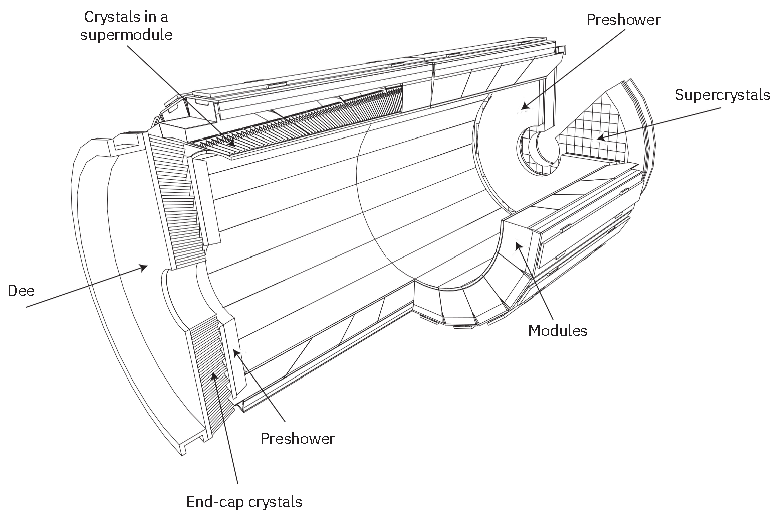
\includegraphics[width= .85\textwidth]{Figures/Chapter3/CMS_ECAL.pdf}
\caption[Schematic view of the CMS ECAL subdetector]{Schematic view of the CMS ECAL subdetector. Figure taken from Ref.~\cite{LHC_CMS}.}
\label{Figure:Chapter3_CMS_ECAL}
\end{figure}
\newpage
The energy resolution of the ECAL is parametrised as a function of the incident particle energy $E$ as:

\begin{equation_pad}
    \left(\frac{\sigma}{E}\right)^2 =  \underbrace{\left(\frac{S}{\sqrt{E}}\right)^2}_{\text{Stochastic}} +  \underbrace{\left(\frac{N}{E}\right)^2}_{\text{Noise}} +  \underbrace{C^2}_{\text{Constant}}
\end{equation_pad}

Each term reflects a different contribution to the resolution: the stochastic term accounts for statistical fluctuations in lateral shower containment and photon yield; the noise term reflects electronic noise and PU; and the constant term arises from detector non-uniformities ($\eg$ longitudinal response) and calibration uncertainties. During an electron test beam in 2014~\cite{ECAL_TestBeam}, the ECAL demonstrated excellent energy resolution, consistent with the design specifications:

\begin{equation_pad}
    \left(\frac{\sigma}{E}\right)^2 =  \underbrace{\left(\frac{2.8\%}{\sqrt{E}}\right)^2}_{\text{Stochastic}} +  \underbrace{\left(\frac{0.12}{E}\right)^2}_{\text{Noise}} +  \underbrace{(0.30\%)^2}_{\text{Constant}}
\end{equation_pad}

\subsection{Hadronic calorimeter}
To complete the calorimetric measurement and ensure accurate reconstruction of hadronic jets and \ac{MET}, the CMS detector employs a dedicated HCAL system. Positioned outside the ECAL, the HCAL is a sampling calorimeter designed to detect strongly interacting particles and spans the pseudorapidity range $|\eta| < 5.2$~\cite{LHC_CMS,CMS_Detector_Run3}. The HCAL comprises four distinct components: the \ac{HB}, \ac{HE}, \ac{HO}, and \ac{HF} calorimeters, as shown in Fig.~\ref{Figure:Chapter3_CMS_HCAL}.

\begin{figure}[h]
\centering
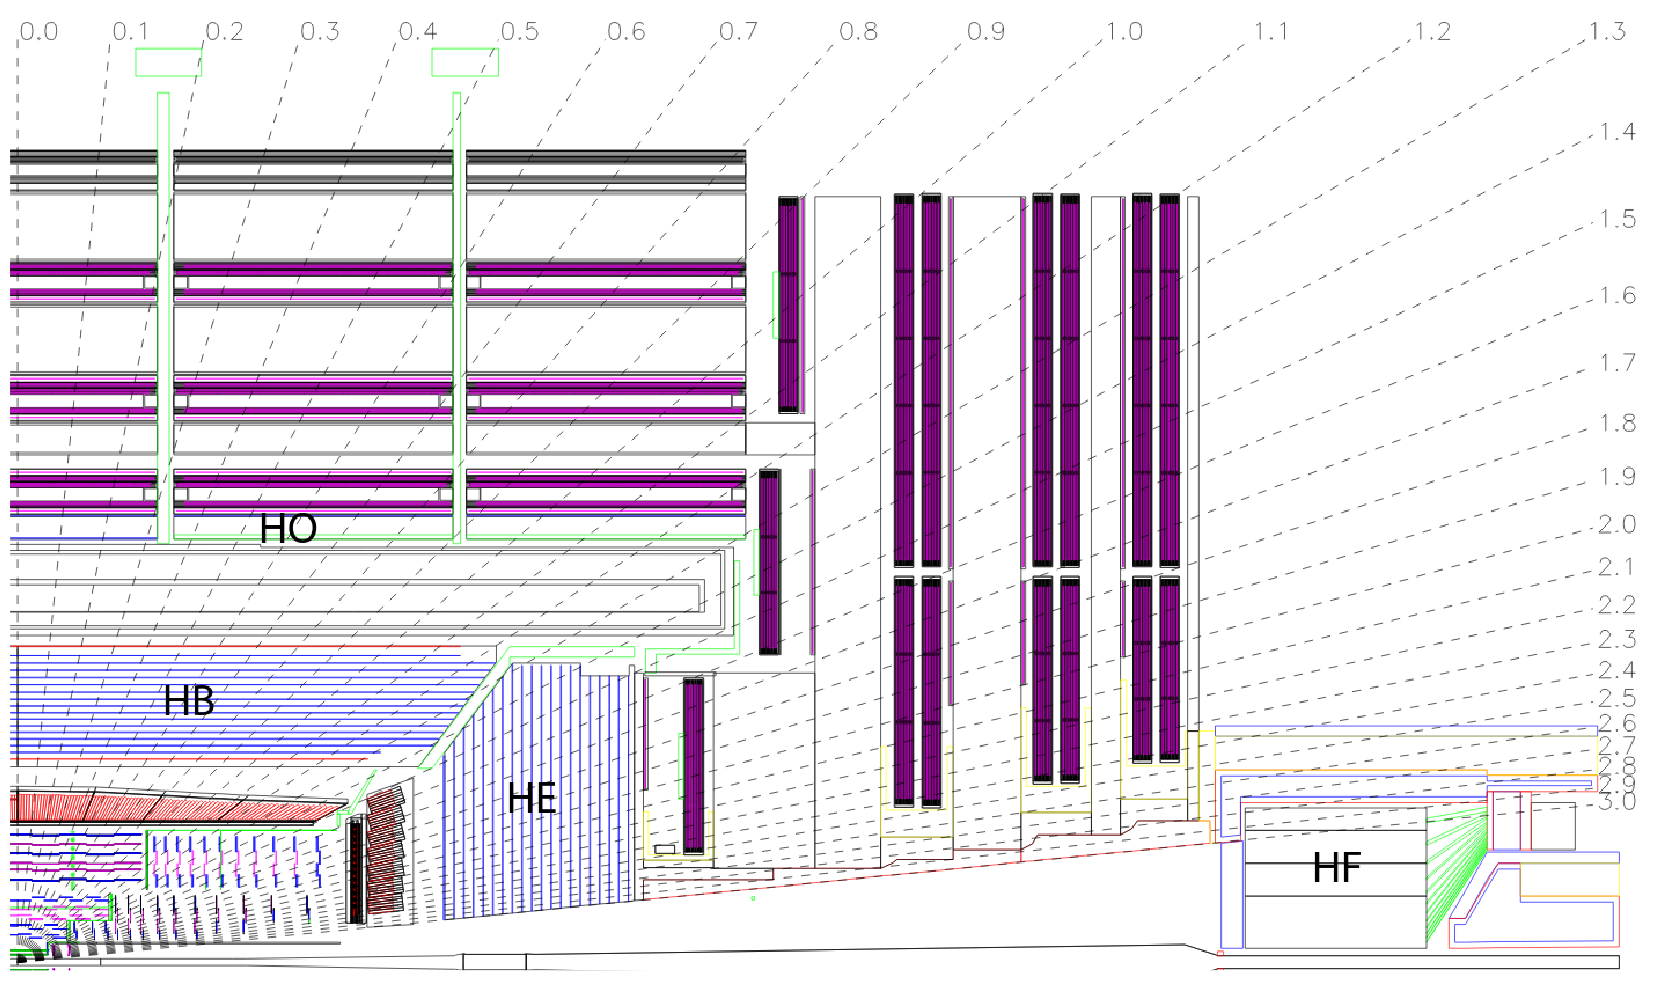
\includegraphics[width= 1.0\textwidth]{Figures/Chapter3/CMS_HCAL.pdf}
\caption[Schematic of CMS detector highlighting HCAL sub-detectors]{A schematic view of one-quarter of the CMS detector with the locations of the HB, HO, HE and HF sub-detectors of the HCAL being shown. Figure adjusted from Ref.~\cite{LHC_CMS}.}
\label{Figure:Chapter3_CMS_HCAL}
\end{figure}

The \textbf{HB} and \textbf{HE} subdetectors are located within the bore of the magnet, covering the pseudorapidity regions $|\eta| < 1.3$ and $1.3 < |\eta| < 3.0$, respectively. They are constructed using alternating layers of brass absorber plates and plastic scintillators. Brass is used due to its short nuclear interaction length and non-magnetic nature, the latter being essential for operation within the CMS solenoid. The HB has a minimum absorber thickness of 5.82 interaction lengths ($\lambda_0$), which increases with polar angle as ($1/\sin\theta$) to approximately 10.6~$\lambda_0$ at $|\eta| = 1.3$. In the \textbf{HE}, 79$\unit{mm}$ thick brass plates interleaved with 9$\unit{mm}$ scintillator gaps provide a total depth of around 10$\lambda_0$, including the contribution from the electromagnetic crystals in front. The calorimeter segmentation is $\Delta\eta \times \Delta\phi = 0.087 \times 0.087$ for $|\eta| < 1.6$, and approximately $0.17 \times 0.17$ for $|\eta| \geq 1.6$. Charged particles from hadronic showers deposit energy in the scintillator tiles, producing scintillation light that is collected by wavelength-shifting fibres and read out using hybrid photodiodes.

Due to the solenoid magnet, the HB is radially restricted, constraining the total amount of material which can be inserted to absorb hadronic showers. As a result, the combined stopping power of the EB and HB does not provide sufficient containment of the hadronic showers. The \textbf{HO} subdetector is used as a tail catcher outside of the solenoid, aiming to ensure adequate sampling depth for $|\eta| < 1.3$. The HO employs the same active scintillator as the HB, while also utilising the solenoid as an additional absorber, extending the minimum depth to 11.8$\lambda_0$. This extended sampling is crucial for identifying and measuring the energy of late-starting or highly penetrating showers.

Beyond $|\eta| < 3.0$, the \textbf{HF} sub-detector extends the pseudorapidity coverage of the CMS HCAL to $|\eta| < 5.2$, and is located at $\pm 11.2\unit{m}$ from the interaction point. Its design posed significant challenges due to the extremely harsh radiation environment in the forward region, where particle fluxes reach unprecedented levels. To ensure long-term durability, the HF was constructed using highly radiation-resistant materials. Quartz fibres were chosen as the active medium, embedded within a steel absorber composed of 5$\unit{mm}$ thick grooved plates into which the fibres are inserted. The HF subdetector is segmented longitudinally into two readout depths: one set of fibres spans the entire 165$\unit{cm}$ depth of the absorber (approximately 10~$\lambda_0$), while the other begins at a depth of 22$\unit{cm}$. By reading out these fibre sets independently, the HF can discriminate between electromagnetic showers, which deposit a large fraction of their energy in the first $22\unit{cm}$ and hadronic showers, which deposit their energy more uniformly across the full depth. When charged particles pass through the quartz fibres, they produce Cherenkov light, which is then collected and transmitted to photomultiplier tubes. The use of Cherenkov light makes the HF relatively insensitive to low-energy particles and neutral backgrounds, such as neutrons or secondary products from activated radionuclides, helping to reduce noise in this high-radiation environment.

When combining information from the inner tracking system with measurements from the calorimeters, the jet energy resolution typically reaches 15\% at $10\unit{GeV}$, 8\% at $100\unit{GeV}$, and 4\% at $1\unit{TeV}$. In comparison, using only the ECAL and HCAL calorimeters yields resolutions of approximately 40\%, 12\%, and 5\% at the same energies, respectively~\cite{CMS_HCAL_EnergyResolution}.

\subsection{Muon system}
To satisfy the LHC’s stringent performance goals for muon reconstruction, CMS employs a dedicated muon tracking system~\cite{LHC_CMS,CMS_Muon_System_Performance} positioned furthest from the interaction point. The system serves three primary functions: muon identification, momentum measurement, and triggering. These are made possible by the strong solenoidal magnetic field and the iron return yoke, which acts as a hadron absorber.  CMS employs three complementary gaseous particle detector technologies for detecting muons.  

In the barrel region, where muon rates and neutron-induced backgrounds are relatively low, the $3.8–4\unit{T}$ magnetic field is uniform and largely confined within the iron yoke. \textbf{\ac{DTs}} are used here, providing coverage in the pseudorapidity region $|\eta| < 1.2$. These are organised into four stations interspersed among the layers of the flux return plates. The first three stations are further subdivided into eight chambers, four measuring the muon coordinate in the $r-–\phi$ bending plane and four providing a measurement in the $z$ direction. Conversely, the capabilities of the fourth muon station are restricted to $r–-\phi$ measurements. Each DT chamber consists of rectangular drift cells containing a central anode wire. The cells are filled with a gas mixture of argon and carbon dioxide, which enables efficient ionisation and drift of electrons toward the wire for signal detection. 

In contrast to the barrel region, the endcaps are subjected to higher muon rates and background levels. The magnetic field in this region is both strong and non-uniform, necessitating a finely segmented detector system that is radiation-resistant and capable of fast response times. To meet these demands, CMS employs \textbf{\ac{CSCs}} in the region $0.9 < |\eta|<2.4$. Each CSC is a multi-layered gaseous detector consisting of six planes of anode wires interleaved with seven cathode layers. In both endcaps, the chambers are arranged into four stations placed perpendicular to the beam line and embedded between the layers of the iron yoke. The cathode strips extend radially outward from the beam axis, providing precise position measurements in the $r-\phi$ plane. The anode wires, oriented roughly perpendicular to the strips, deliver additional spatial information in $\eta$ and enable timing measurements relative to the beam crossing. This six-layer configuration enhances pattern recognition, improving the rejection of spurious hits from background sources and allowing for efficient correlation with hits from other stations and with tracks reconstructed in the inner tracker.

The DT and CSC systems are complemented by the \textbf{\ac{RPC}} system in the pseudorapidity region $|\eta| < 1.6$. RPCs are double-gap chambers featuring anode and cathode plates separated by gas. Compared to DTs and CSCs, RPCs exhibit lower granularity; however, they offer a faster response and good time resolution. These characteristics make them particularly well-suited for use as trigger detectors. As such, they are especially valuable in scenarios where the DT and CSC systems may struggle to cope with PU-induced background. Additionally, RPCs contribute to resolving ambiguities when reconstructing tracks from multiple hits within a chamber, further enhancing the overall performance of the muon detection system.

A schematic illustration of the CMS muon detection system is shown in Fig.~\ref{Figure:Chapter3_CMS_Muon_System}, highlighting the arrangement of the DT, CSC, and RPC subdetectors within the return yoke. Owing to its design, the CMS muon system achieves a reconstruction and identification efficiency exceeding 95\% for muons with energies above a few $\unit{GeV}$. The momentum resolution varies between 1\% and 6\% for transverse momenta below $100\unit{GeV}$, and remains better than 10\% up to $1\unit{TeV}$~\cite{CMS_Muon_System_Performance_2}. Furthermore, the system reliably determines the muon charge sign for transverse momenta up to $1\unit{TeV}$.


\begin{figure}[h]
\centering
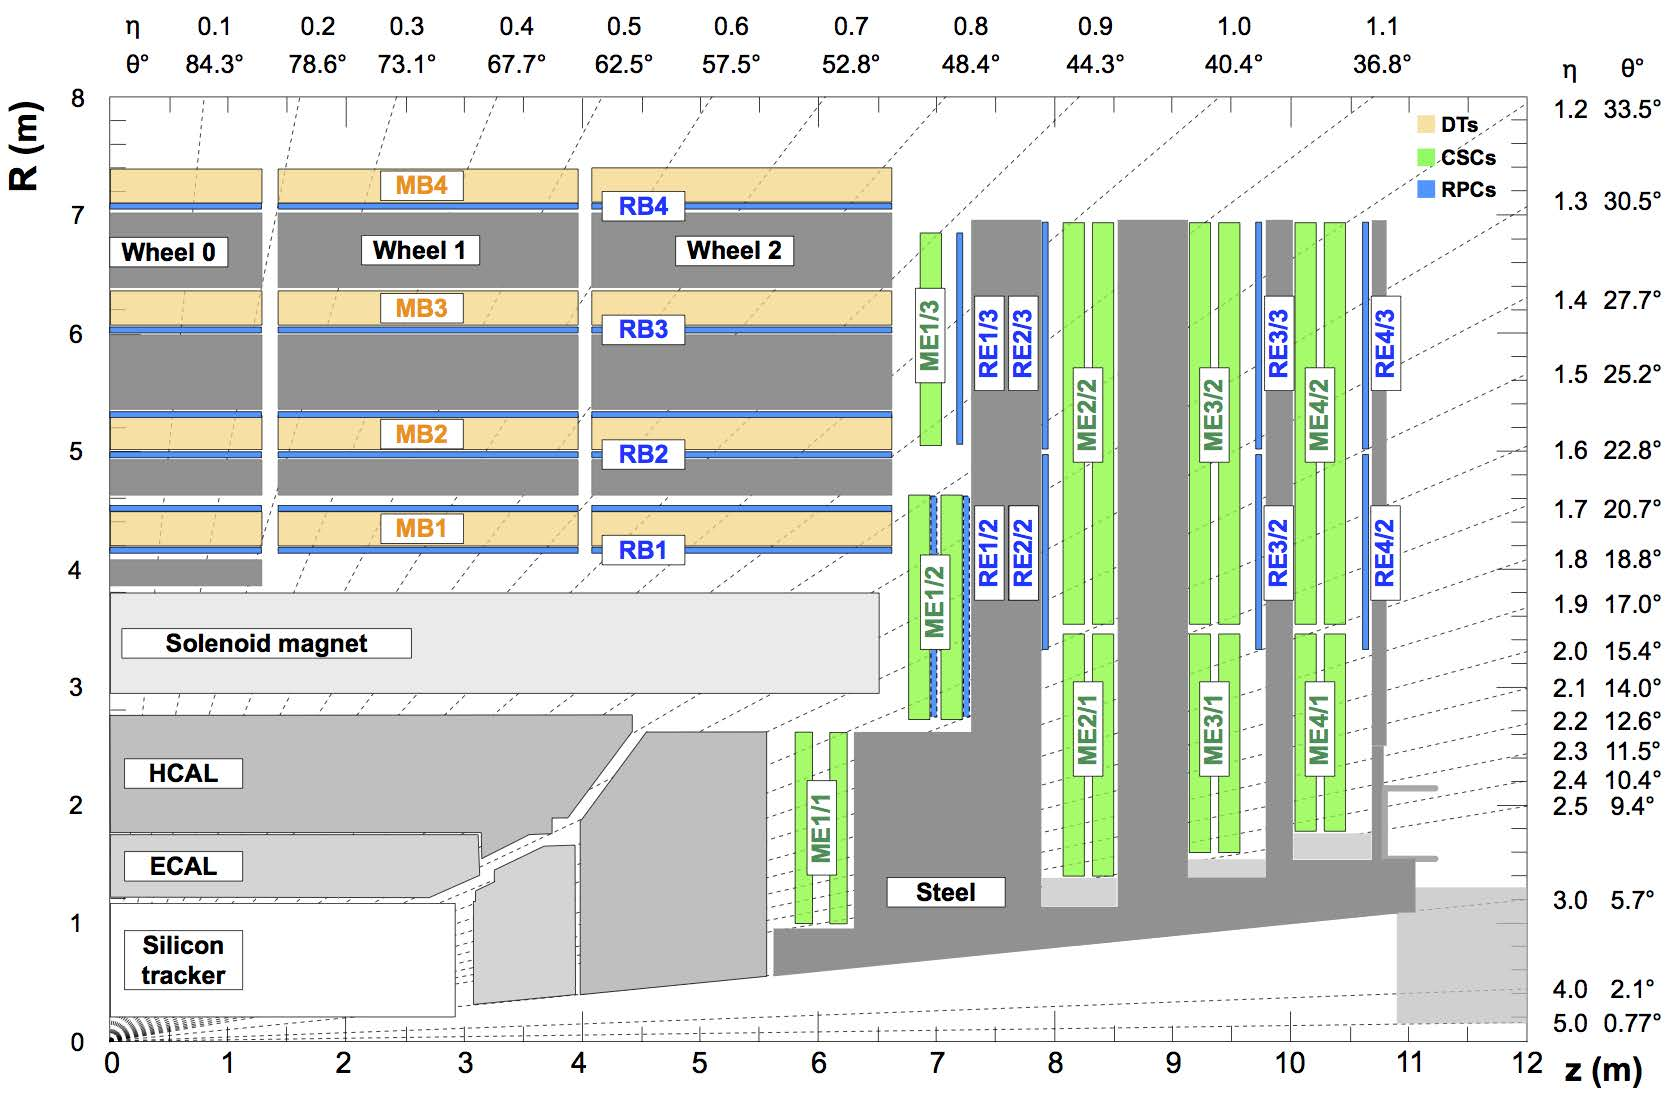
\includegraphics[width= 1.0\textwidth]{Figures/Chapter3/CMS_Muon_System.pdf}
\caption[Schematic of CMS muon detection system]{Schematic illustration of one quarter of the CMS detector, highlighting the muon detection system. The DT stations are labelled as MB (Muon Barrel), while the CSCs are labelled as ME (Muon Endcap). The RPCs are denoted as RB in the barrel region and RE in the endcap region. Figure taken from Ref.~\cite{CMS_Muon_System_Performance}.}
\label{Figure:Chapter3_CMS_Muon_System}
\end{figure}

\subsection{Trigger system}

At the LHC interaction points, proton bunches cross every $25\unit{ns}$, resulting in a nominal bunch crossing frequency of $40\unit{MHz}$. Additionally, each bunch crossing can yield up to more than 50~PU interactions corresponding to an aggregate rate of individual proton-proton interactions surpassing $1\unit{GHz}$. Recording all of these collisions is not feasible nor necessary, as only a small fraction contains events of interest to the CMS physics programme. To select the most interesting events, CMS employs a dedicated two-level trigger system~\cite{CMS_Trigger} consisting of the \textbf{\ac{L1} trigger} and the \textbf{\ac{HLT}}.

As the name suggests, the \textbf{L1 trigger} is the first level of the CMS trigger system, implemented as a hardware-based trigger on custom-built Field Programmable Gate Arrays with a fixed latency of $4\unit{\mu s}$. CMS relies on this system to rapidly determine whether an event should be tentatively accepted or rejected based on calorimeter energy deposits and muon detector hits. The L1 decision chain comprises three primary subsystems: the L1 calorimeter system, the L1 muon trigger system and the global trigger (GT), as shown in Fig.~\ref{Figure:Chapter3_CMS_L1_Trigger}.

\begin{figure}[h]
\centering
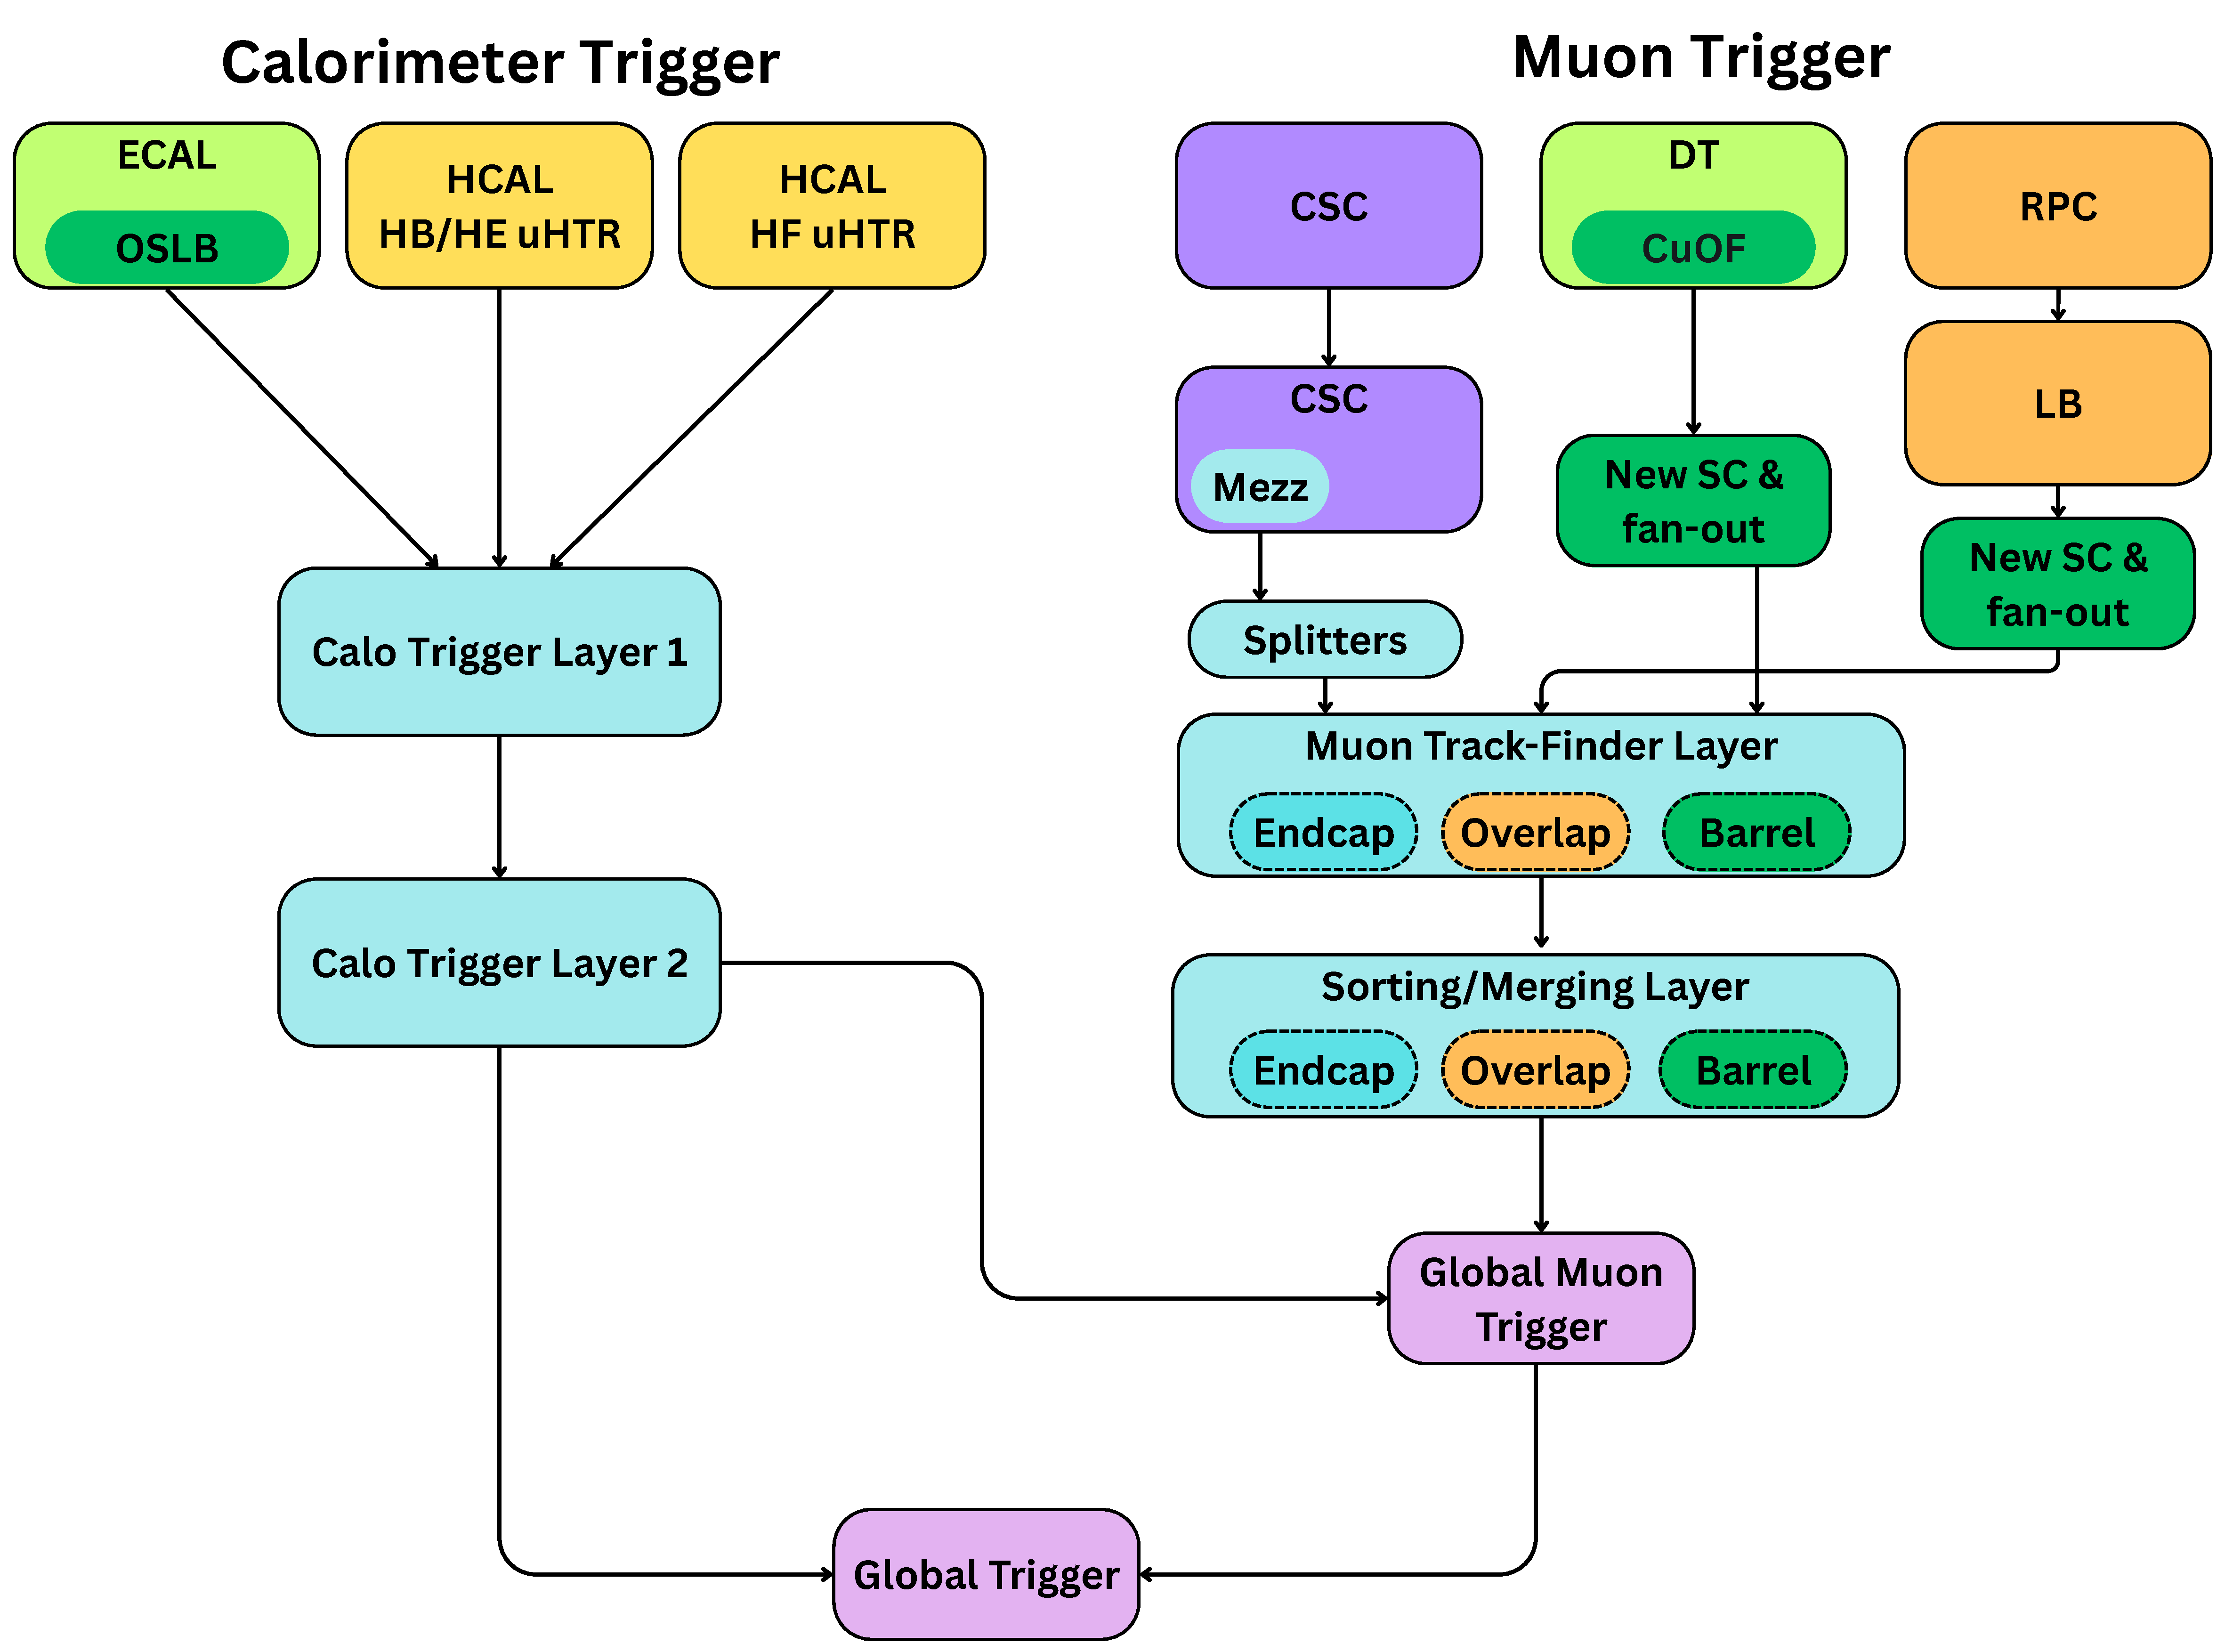
\includegraphics[width= 1.0\textwidth]{Figures/Chapter3/CMS_L1_Trigger.pdf}
\caption[Schematic of the CMS L1 trigger workflow]{Schematic of the CMS L1 trigger workflow. Figure reproduced from Ref.~\cite{CMS_L1_Trigger}.}
\label{Figure:Chapter3_CMS_L1_Trigger}
\end{figure}

The \textbf{L1 calorimeter trigger system} is organised into two processing layers. Layer-1 (\textit{Calo Trigger Layer 1}) receives trigger primitives (energy deposits) from the ECAL and the HCAL, performs initial calibrations, and sorts local energy deposits. Layer-2 (\textit{Calo Trigger Layer 2}) processes the calibrated information to reconstruct and further calibrate high-level physics objects such as electrons, photons, jets, taus, and MET. Simultaneously, hits from the three muon subsystems are processed by the first stage of the \textbf{L1 muon trigger system} (\textit{Muon Tracking-Finder Layer}). At this stage, track finding is performed by combining hits within sectors in $\phi$ and $\eta$. The reconstructed track candidates are then forwarded to the \textit{Sorting and Merging Layer}, where information from the $\phi$ sectors is consolidated. The output, along with the calorimeter information required to compute isolation, is passed to the global muon trigger, where a sorted list of muon candidates for the entire detector is produced. Finally, the \textbf{global trigger} integrates the information from both the L1 calorimeter and muon trigger systems, enabling it to make a decision on the fate of the event. This allows for the event rate to be reduced from $40\unit{MHz}$ to $100\unit{kHz}$.

The \textbf{HLT} system is the second stage of the CMS trigger architecture. It is a software-based trigger that runs on a processor farm composed of commercial CPUs. In contrast to the hardware-based L1 trigger, the HLT utilises full-resolution data from the CMS detector and applies offline-quality reconstruction algorithms for more refined event selection. The primary objective of the HLT is to further reduce the event rate to about $1\unit{kHz}$ for permanent storage and offline analysis. 

Rather than operating with fixed latency, the HLT processes events asynchronously, scaling with available CPU resources. Its workflow is organised into HLT paths, each consisting of a predefined sequence of algorithmic steps that reconstruct and select physics objects. These paths are structured to increase in complexity, precision, and physics sophistication. To optimise computational efficiency, initial selections use fast information from the calorimeters and muon detectors, while CPU-intensive tracking is applied only to events that pass these preliminary filters. 

Events accepted by the HLT are handed off to the storage manager, which writes them temporarily to local disk. They are then transferred to the CMS Tier‑0 computing centre for offline reconstruction and long‑term archival.



\setcounter{mtc}{4}
\chapter{XXXXXX}
\chaptermark{XXXXX}  
\thispagestyle{plain}  % First page has default style
\pagestyle{chapterpages}
\label{Section:Chapter4}

\minitoc

hey hey
\setcounter{mtc}{5}
\chapter{Redefining the CMS Data Format}
\chaptermark{Redefining the CMS Data Format}
\thispagestyle{plain}  % First page has default style
\pagestyle{chapterpages}
\label{Section:Chapter5}
\minitoc

Within the CMS computing model, the \textbf{RAW} data format represents the full detector output and is the first available offline copy of an event following its acceptance by the HLT. It contains ``raw'' detector information, the L1 trigger result, the result of the HLT selections and other metadata.  The \textbf{RECO} format is derived from this complete record, and is the most CPU-intensive part of the CMS data processing chain because it involves reconstructing physics objects. This is followed by the \textbf{AOD} data format, a ``distilled" version of RECO designed to enable a broad range of physics analyses. Beyond AOD, CMS provides increasingly compact data formats, each offering different levels of information and precision.

The motivation to improve the RAW data format stems from the growing demands on the CMS data processing system. One of the primary challenges is the increasing complexity of events resulting from higher PU conditions. This complexity has a direct impact on the size of RAW events, imposing considerable strain on storage and bandwidth.  On average, RAW data currently occupies around $1.5\unit{MB}$ per event for pp collision data and approximately $2\unit{MB}$ per event for simulated events, with size expected to scale approximately linearly with PU. Therefore, it is necessary to explore improvements or data-reduction strategies for the RAW data format to prepare CMS for the higher PU conditions anticipated in future runs. 

This chapter will outline the main contributor to event size in the current RAW data format. This will be followed by the most recent data-reduction developments introduced in an alternative format, referred to as \textbf{RAW'}.

\section{Impact of the Silicon Strip Tracker on RAW size}
The \textbf{RAW} data format is constructed by collecting data fragments from all CMS subdetectors and assembling them into complete events. These fragments are read out by FEDs, which digitise the analogue signals and perform initial digital processing before passing the data to the event builder. Each subdetector is served by a number of FEDs, with the number depending on the its complexity and channel count.

The tracking subdetectors contribute the largest share of data to the RAW data format due to their exceptionally high channel density compared to other CMS subdetectors. In particular, the SST is the dominant contributor corresponding to roughly $\sim 50\%$ of the RAW event size because of the large number of FEDs dedicated to its readout. An overview of the number of channels and associated FEDs for all CMS subdetectors is provided in Table~\ref{Table:Chapter4_RAW_Channels_FED}.

\begin{table}[htbp]
\centering
\renewcommand{\arraystretch}{1.5} % Increase row height
\begin{tabular}{|l|c|c|}
\hline
Subdetector & Number of Channels & Number of FEDs \\
\hline \hline
Pixel tracker & $\sim124\unit{M}$ & 108 \\
\arrayrulecolor{lightgray} \hline
Strip tracker & $\sim9.3\unit{M}$ & 440 \\
\arrayrulecolor{lightgray} \hline
Preshower & $\sim144\unit{k}$ & 56 \\
\arrayrulecolor{lightgray} \hline
ECAL & $\sim75\unit{k}$ & 54 \\
\arrayrulecolor{lightgray} \hline
HCAL & $\sim9\unit{k}$ & 32 \\
\arrayrulecolor{lightgray} \hline
Muons CSC & $\sim500\unit{k}$ & 8 \\
\arrayrulecolor{lightgray} \hline
Muons RPC & $\sim192\unit{k}$ & 3 \\
\arrayrulecolor{lightgray} \hline
Muons DT & $\sim195\unit{k}$ & 10 \\
\arrayrulecolor{lightgray} \hline
\arrayrulecolor{black} \hline
\end{tabular}
\caption[CMS subdetector read-out parameters]{CMS subdetector read-out parameters. Values extracted from Ref.~\cite{LHC_CMS,CMS_Tracker_Phase1_Upgrade_2}.}
\label{Table:Chapter4_RAW_Channels_FED}
\end{table}

Given the significant contribution of the SST to the overall RAW event size, a promising strategy for data reduction is to optimise the information retained from the FED output. As discussed in Section~\ref{Section:Chapter4_Reconstruction_of_PF_elements}, clusters in the tracker are formed from contiguous strips with signal above predefined thresholds. For each cluster, the information stored in the RAW data includes the index of the first strip in the cluster and the ADC amplitudes for each strip within the cluster. Hence, exploring alternative representations of cluster information in the RAW data may offer additional opportunities for reducing the SST data volume.

\section{RAW' Data Format: Iteration 1}
\label{Section:Chapter5-RAW'_Iteration_1}
Reducing cluster-level information invites a key question: \textit{how much information can be discarded without compromising the accuracy of reconstructed physics observables?} To address this question, it is essential to consider the physical meaning encoded in the shape and structure of each cluster. 

A strip cluster represents a localised charge distribution induced by a charge particle traversing the subdetector. This distribution is typically non-uniform, exhibiting a peak where the maximum charge is deposited, along with signal tails extending over adjacent strips. Additionally, the particle's angle of incidence, entry point, and trajectory through the silicon sensor can introduce asymmetries in the charge distribution. The width of the cluster can also vary, with clusters associated with reconstructed tracks (on-track clusters) typically being narrower and more symmetric than those not linked to any track (off-track clusters).

Despite this complexity, the full cluster shape may not always be necessary to retain. It is therefore reasonable to consider whether a simplified, symmetric distribution could approximate the underlying charge profile while preserving the essential physics information. To evaluate the feasibility of such approximations, statistical measures such as skewness and kurtosis are used to characterise the shape of the cluster's charge distribution. These measurements are performed in different collision environments, including events with high jet activity, energetic isolated muons, and minimally biased pp collisions. Skewness values are typically close to zero or slightly positive ($\sim 0.23$), indicating only mild asymmetry. Additionally, kurtosis offers insight by quantifying the peakedness and tail behaviour of the distributions. In particular, Fisher kurtosis~\cite{Kurtosis}\footnote{The kurtosis of a standard normal distribution is three. Fisher kurtosis is a modified version of the standard Pearson kurtosis, normalising the Gaussian distribution to have a kurtosis of zero. This makes it easier to interpret deviations from normality: positive values indicate heavier tails (leptokurtic), and negative values indicate flatter distributions (platykurtic).} reveal that strip charge distributions are generally platykurtic, with values around -1.6. This is comparable to a uniform (rectangular) distribution, which has a Fisher kurtosis of -1.2.

These observations suggest that much of the cluster structure can be effectively summarised using a reduced set of parameters.  In the \textit{RAW'} data format, the per-strip ADC count (charge) is replaced with a \textit{simplified rectangular approximation} that preserves the original cluster width. The information stored per cluster consists of:

\begin{itemize}
    \item \textbf{Barycenter}: The charge-weighted centre of the cluster, serving as an approximation of the point at which the particle traversed the subdetector.
    \item \textbf{Width}: The number of strips forming the cluster.
    \item \textbf{Average charge}: The total charge (sum of ADC counts) in the cluster divided by the width of the cluster.
\end{itemize}

In the \textbf{RAW'} data format, the SST contribution to the event size is reduced to approximately 70\% of its original size. This corresponds to an overall event size reduction of approximately 20–25\% compared to the original \textbf{RAW} data format.

\subsection{Tracking performance}

While this new data format provides a significant reduction in the SST data volume, its viability ultimately depends on whether it preserves the physics performance necessary for CMS analyses. Therefore, it is essential to verify that this reduced cluster representation does not degrade the quality of track reconstruction. This can be assessed through the \textit{tracking efficiency}, defined as the fraction of simulated particles successfully reconstructed. The tracking performance of the RAW' data format is shown in Fig.~\ref{Figure:Chapter5_TrackingPerformance_1}, where comparisons of tracking efficiency as a function of $p_\mathrm{T}$ and $\phi$ are presented relative to the standard RAW format.

\begin{figure}[h]
        \centering
        % First row
        \begin{subfigure}[b]{0.49\textwidth}
            \centering
            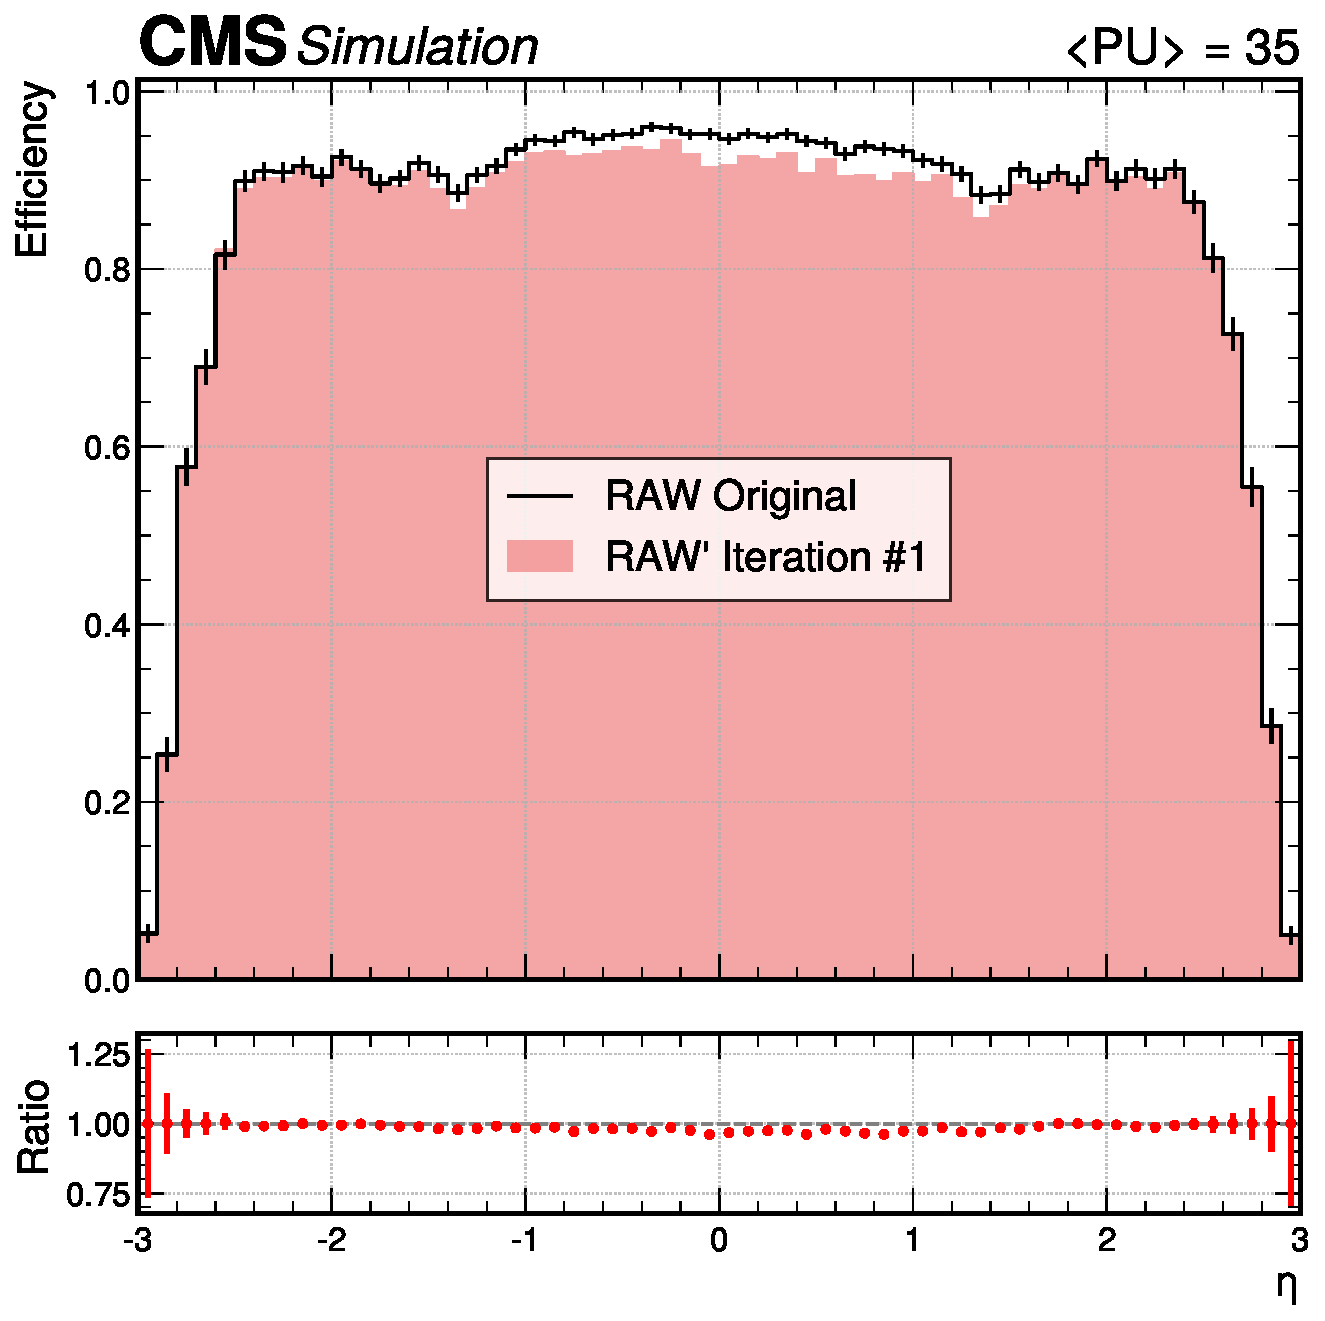
\includegraphics[width=\textwidth]{Figures/Chapter5/efficiency_comparison_1_eta.pdf}
            \caption{}
        \end{subfigure}
        \begin{subfigure}[b]{0.49\textwidth}
            \centering
            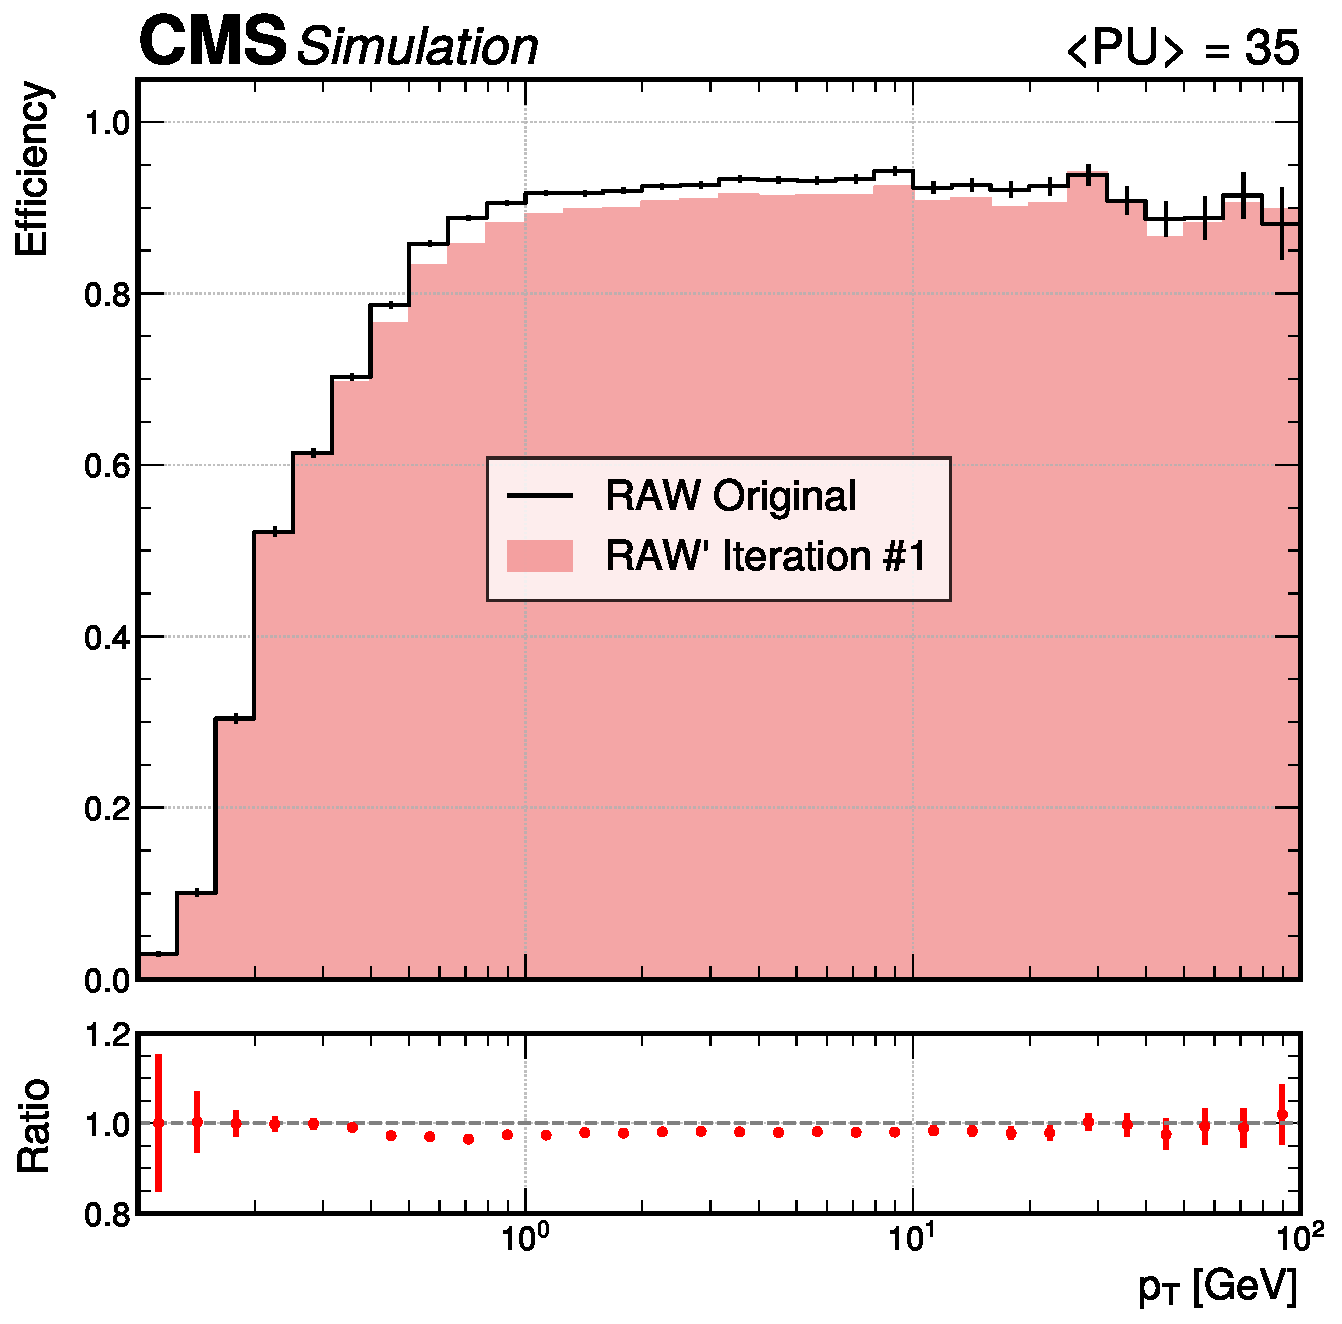
\includegraphics[width=\textwidth]{Figures/Chapter5/efficiency_comparison_1_pt.pdf}
            \caption{}
        \end{subfigure}
    \caption[Comparison of the track reconstruction efficiency as a function of $\eta$ and $p_\mathrm{T}$ between the original RAW format and the first iteration of RAW'.]{Comparison of the track reconstruction efficiency as a function of \textbf{(a)} $\eta$ and \textbf{(b)} $p_\mathrm{T}$ between the original RAW format and the first iteration of RAW'. Results are based on simulated $t\bar{t}$ events.} 
    \label{Figure:Chapter5_TrackingPerformance_1}
\end{figure}

The tracking performance of the RAW' format appears promising, showing a small degradation in efficiency across both $\phi$ and $p_\mathrm{T}$, typically of the order of a few percent. However, it is also important to ensure that this also holds for the efficiency as a function of the vertex radius, as this directly impacts the reconstruction of displaced tracks. As shown in Fig.~\ref{Figure:Chapter5_TrackingPerformance_vertexPos_1}, there is a notable decrease in performance beyond a radius of approximately $10\unit{cm}$, with the efficiency becoming severely degraded above $20\unit{cm}$. 

\begin{figure}[h]
\centering
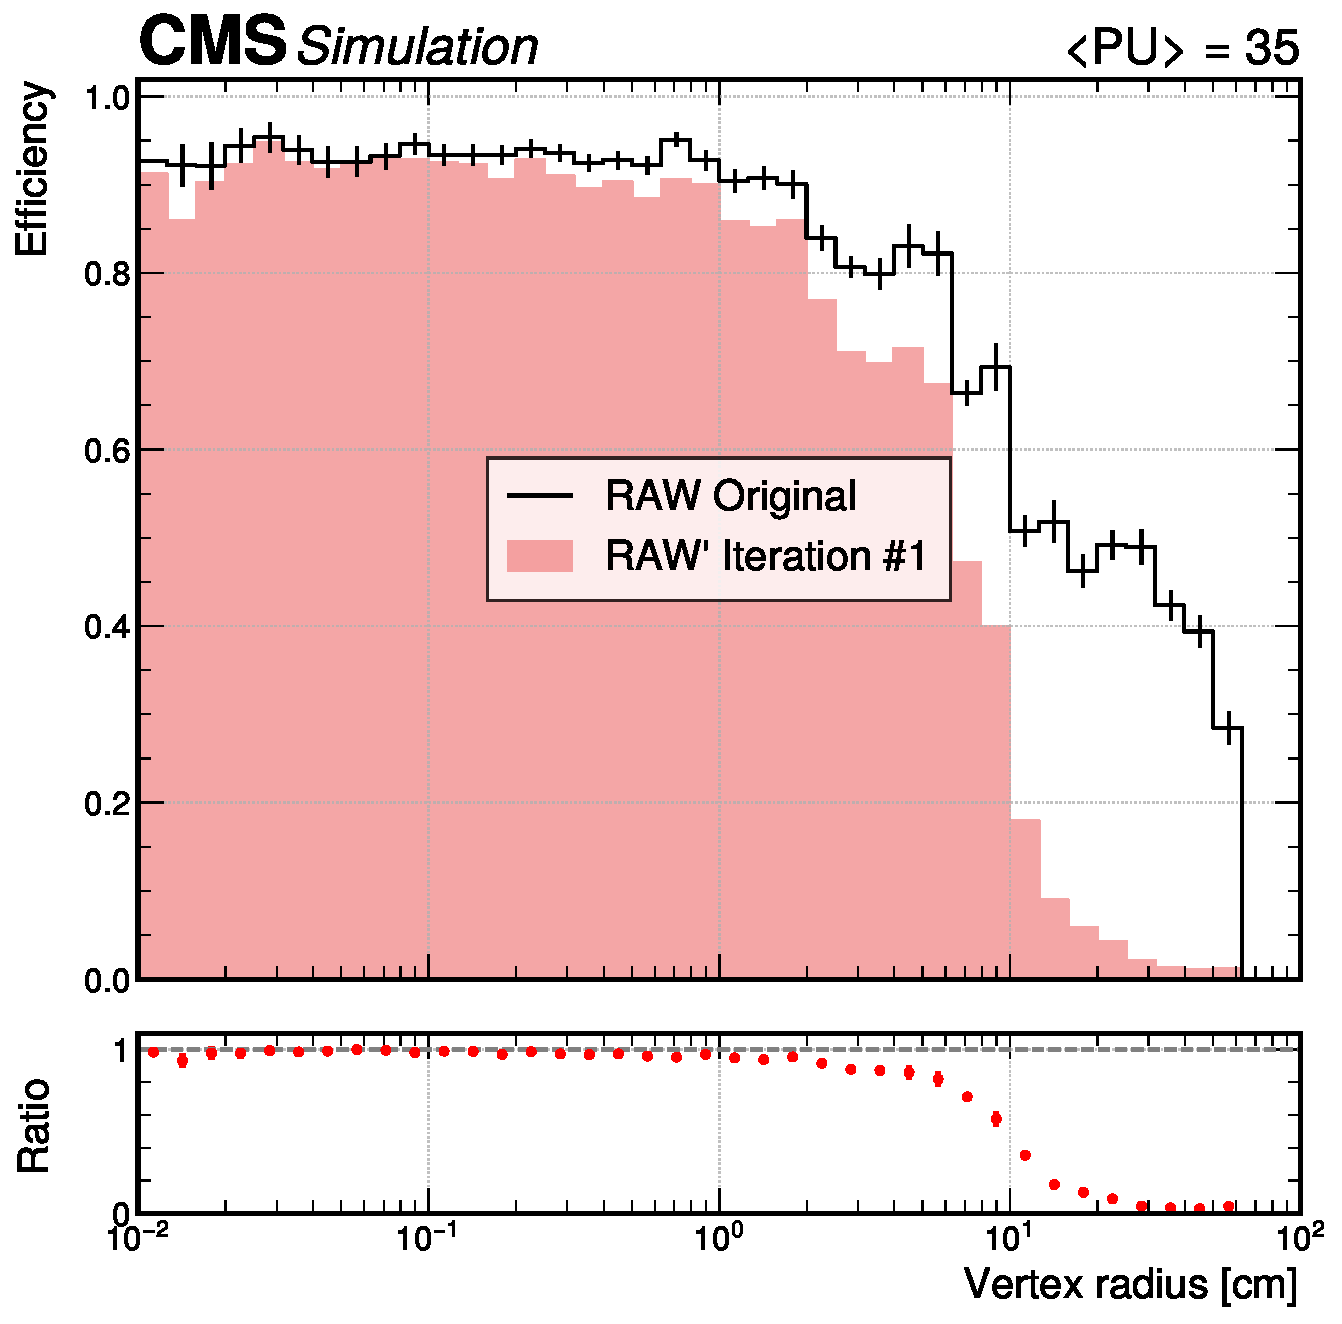
\includegraphics[width=0.8\textwidth]{Figures/Chapter5/efficiency_comparison_1_vertpos.pdf}
\caption[Comparison of the track reconstruction efficiency as a function of the vertex radius between the original RAW format and the first iteration of RAW'.]{Comparison of the track reconstruction efficiency as a function of the vertex radius between the original RAW format and the first iteration of RAW'. Results are based on simulated $t\bar{t}$ events.} 
\label{Figure:Chapter5_TrackingPerformance_vertexPos_1}
\end{figure}

To understand the observed degradation for displaced vertices, Table~\ref{Table:Chapter4_IterativeTrackingSeeds} provides insight into which iterative tracking steps are specifically designed to target such tracks. In particular, the \textit{MixedTriplet}, \textit{PixelLess}, and \textit{TobTec} steps are responsible for reconstructing displaced tracks. By examining the tracking efficiency broken down by iteration step (see Fig.~\ref{Figure:Chapter5_TrackingPerformance_bystep}), it becomes evident that the loss in efficiency at larger radii is primarily due to reduced performance in the PixelLess and TobTec steps.

\begin{figure}[h]
\centering
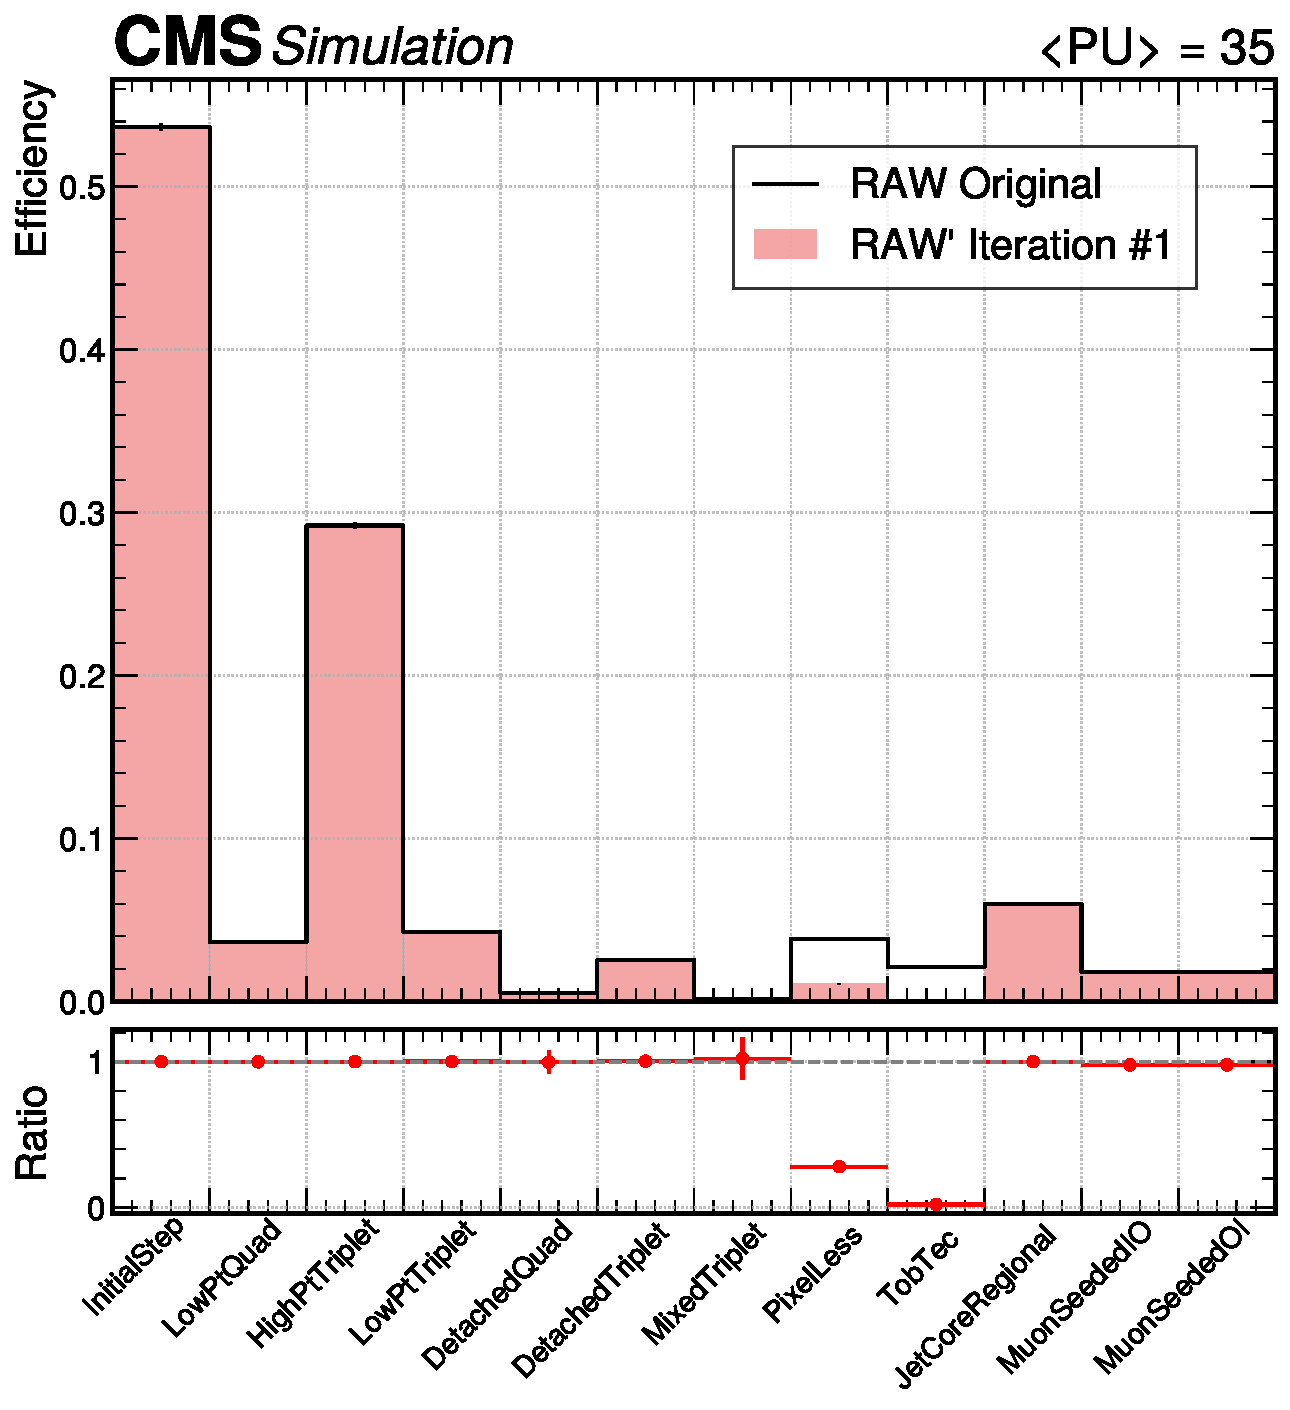
\includegraphics[width=0.8\textwidth]{Figures/Chapter5/efficiency_with_ratio.pdf}
\caption[Track reconstruction efficiency for the different iterations of the CMS iterative tracking algorithm.]{Track reconstruction efficiency for the different iterations of the CMS iterative tracking algorithm. Results are based on simulated $t\bar{t}$ events.}
\label{Figure:Chapter5_TrackingPerformance_bystep}
\end{figure}

\subsection{Complications from cluster shape approximation}

The observed inefficiency in the \textit{PixelLess} and \textit{TobTec} iterations is attributed to the use of cluster shape filters within the CMS iterative tracking algorithm. These filters are particularly effective in the high-combinatorial environment of the CMS tracker, where they help suppress the rate of misreconstructed tracks. However, the rectangular approximation of the cluster charge distribution in RAW' effectively removes the characteristic peaks and tails essential for shape-based discrimination.

One of the first checks performed by the cluster shape filters targets \textbf{saturated strips}. A cluster is flagged as saturated if it contains three consecutive strips with ADC counts above a predefined threshold. However, in this format, only the average cluster charge is stored, rather than the individual strip charges. This approximation can lead to incorrect filter outcomes. For example, if a single strip is sufficiently saturated, this can artificially elevate the average charge of the entire cluster above the saturation threshold, leading to a false positive from the filter. Conversely, clusters that genuinely meet the saturation condition may fail the filter if the average charge falls below the threshold due to dilution from strips with low ADC counts, resulting in a false negative. In comparison to the original format, approximately 99\% of saturated clusters fail this check.

An additional check performed is known as \textbf{trimming}. This step evaluates the presence of tails in the cluster's charge distribution by comparing the charge of each strip to that of neighbouring strips.  This check targets and removes clusters with disproportionately large tails. However, as only the average charge is stored, this filter is rendered ineffective, leading to clusters that would otherwise be rejected being falsely retained. 

Another important check is the presence of a \textbf{peak} in the cluster charge distribution. This step assesses whether the cluster exhibits a clearly defined local maximum. However, there is no local charge variation in this format, causing the filter to fail in detecting a peak within the flat distribution.

\section{RAW' Data Format: Iteration 2}

Motivated by the shortcomings of the initial RAW' format, particularly its inability to retain acceptable track reconstruction efficiency for displaced vertices, a second iteration has been developed. This updated format is specifically designed to address the limitations imposed by cluster shape-based filtering.

The original format of RAW' discussed in Section~\ref{Section:Chapter5-RAW'_Iteration_1} is retained, but a set of additional features is introduced to restore compatibility with cluster shape-based filtering. For the saturated strip check, the solution is straightforward. A boolean flag indicating saturation is computed from the original clusters and stored alongside the barycenter, width and average charge of the cluster. However, the trimming and peak-finding filters are more complex to replicate. This is primarily due to the timing and dependencies of their application within the reconstruction workflow. While the saturated strip check can rely on the original cluster, since the approximated rectangular clusters are constructed directly from it, the trimming and peak-finding filters are applied after cluster construction. At this stage, the original cluster is no longer available. Consequently, these filters cannot ``borrow'' information from the original strip-level data.

In particular, trimming and peak-finding require the estimated position and direction of a track as it passes through a specific detector layer, referred to as trajectory state on surface (TSOS). These quantities are only available once a track has been reconstructed, and cluster construction occurs earlier in the reconstruction chain. Therefore, TSOS-related inputs cannot be computed directly at that stage because no trajectory information exists. As a result, applying these checks during or immediately after clustering would require these track-dependent variables to be approximated or inferred through alternative means.

To address these challenges, the clustering step has been enhanced to incorporate additional information such as the beamspot position, tracker geometry, and noise conditions. With this additional input, basic versions of the trimming and peak filters can now be applied directly during cluster construction. The cluster’s position is estimated using its barycenter, and a vector from the beamspot is used to approximate the track direction toward the cluster. While the use of geometric and noise-related information introduces added complexity, particularly due to local-to-global coordinate transformations, the core structure of the RAW' format remains unchanged. The only addition is a single boolean flag that captures the combined outcome of the saturation, trimming, and peak filters. Despite this extension, the format still achieves a 20\% reduction in data size compared to the original.

\subsection{Tracking performance}

The central question for this updated RAW' format is whether it can recover the tracking inefficiencies introduced by the first version, particularly in reconstructing displaced tracks. Fig.~\ref{Figure:Chapter5_TrackingPerformance_2} shows the tracking efficiency as a function of $p_\mathrm{T}$, $\eta$, and vertex radius. While the first iteration already preserved efficiency reasonably well in $p_\mathrm{T}$ and $\eta$, leaving limited room for improvement, a significant recovery is observed in the vertex radius distribution. The inefficiencies at large displacements, where performance was most severely degraded, are substantially mitigated in this second iteration, demonstrating the effectiveness of reintroducing shape-based filtering logic.

\begin{figure}[h]
        \centering
        % First row
        \begin{subfigure}[b]{0.49\textwidth}
            \centering
            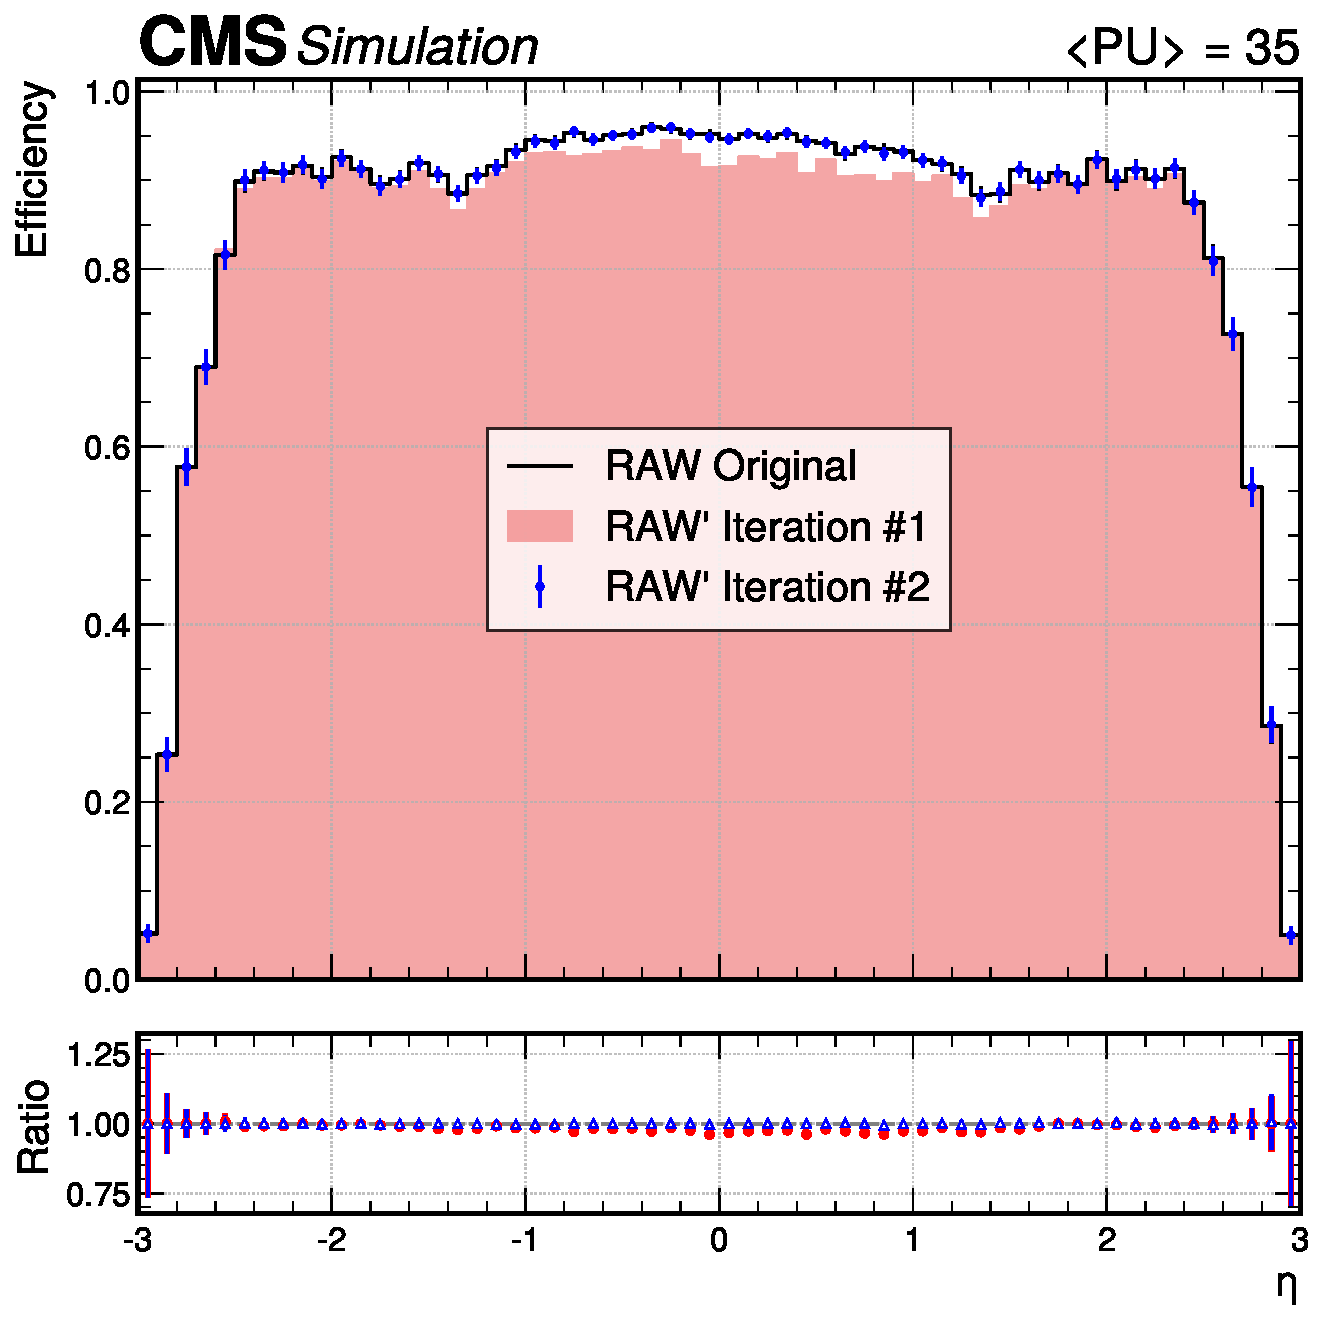
\includegraphics[width=\textwidth]{Figures/Chapter5/efficiency_comparison_2_eta.pdf}
            \caption{}
        \end{subfigure}
        \begin{subfigure}[b]{0.49\textwidth}
            \centering
            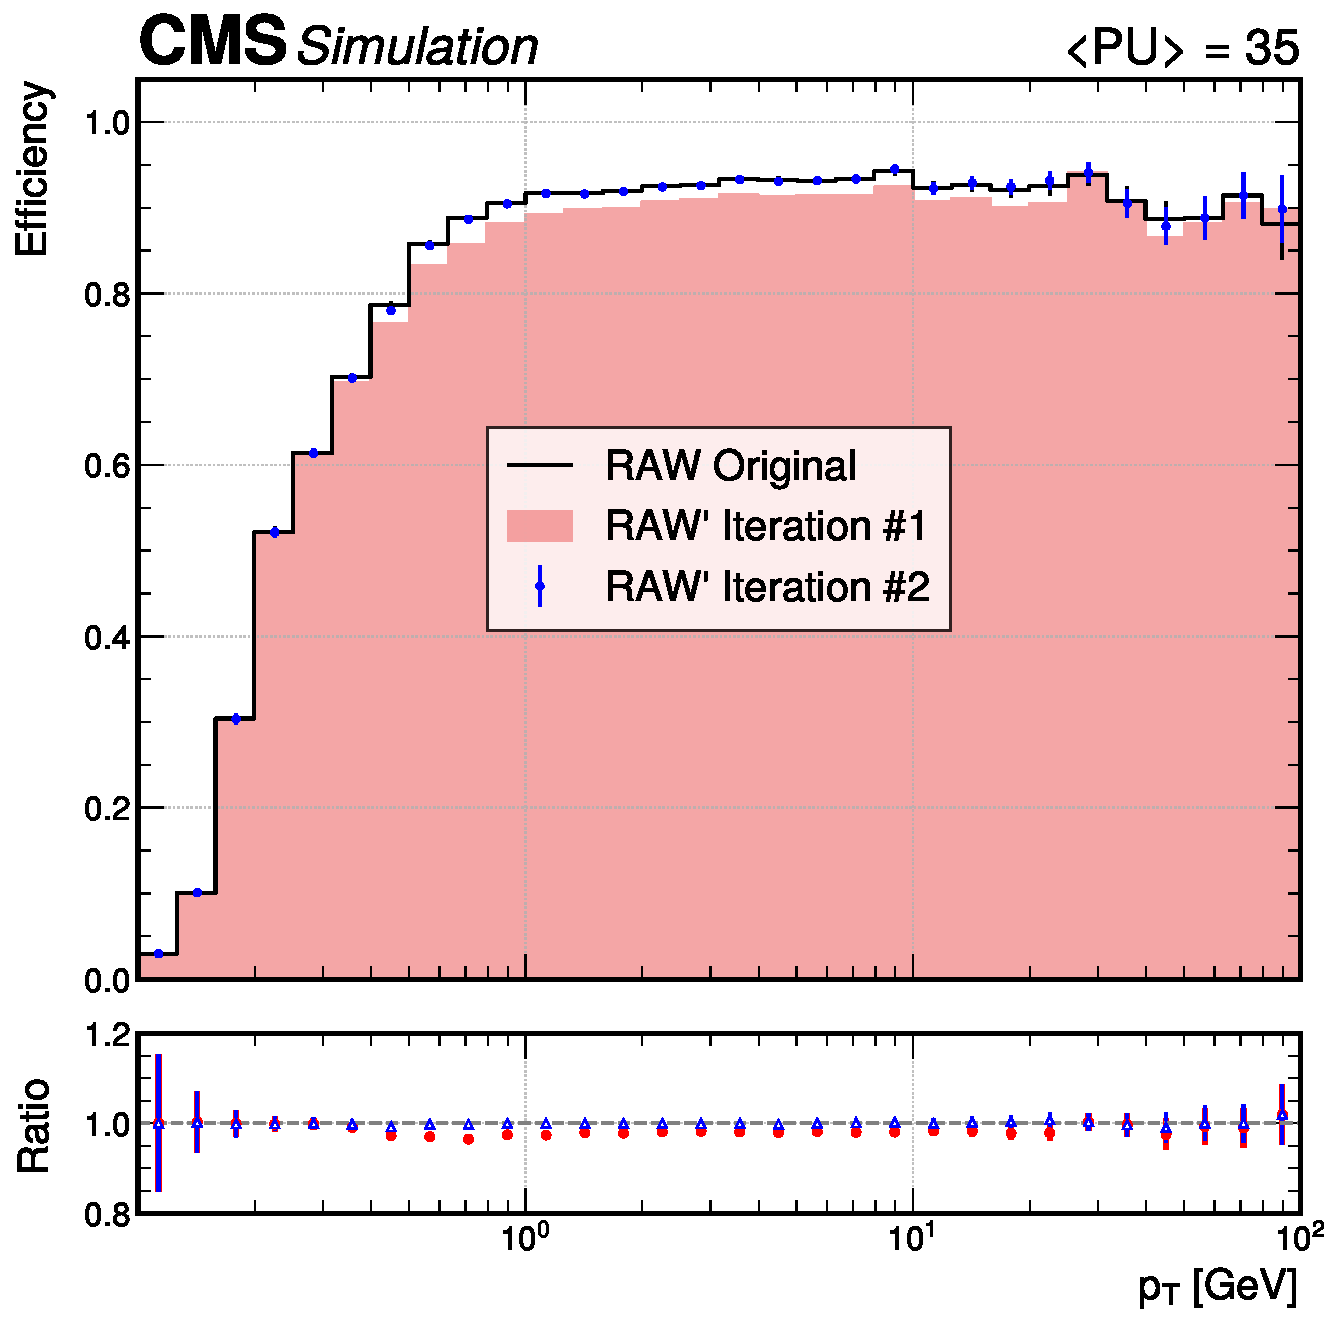
\includegraphics[width=\textwidth]{Figures/Chapter5/efficiency_comparison_2_pt.pdf}
            \caption{}
        \end{subfigure}

        \vspace{0.5cm}

        \begin{subfigure}{0.49\textwidth}
            \centering
            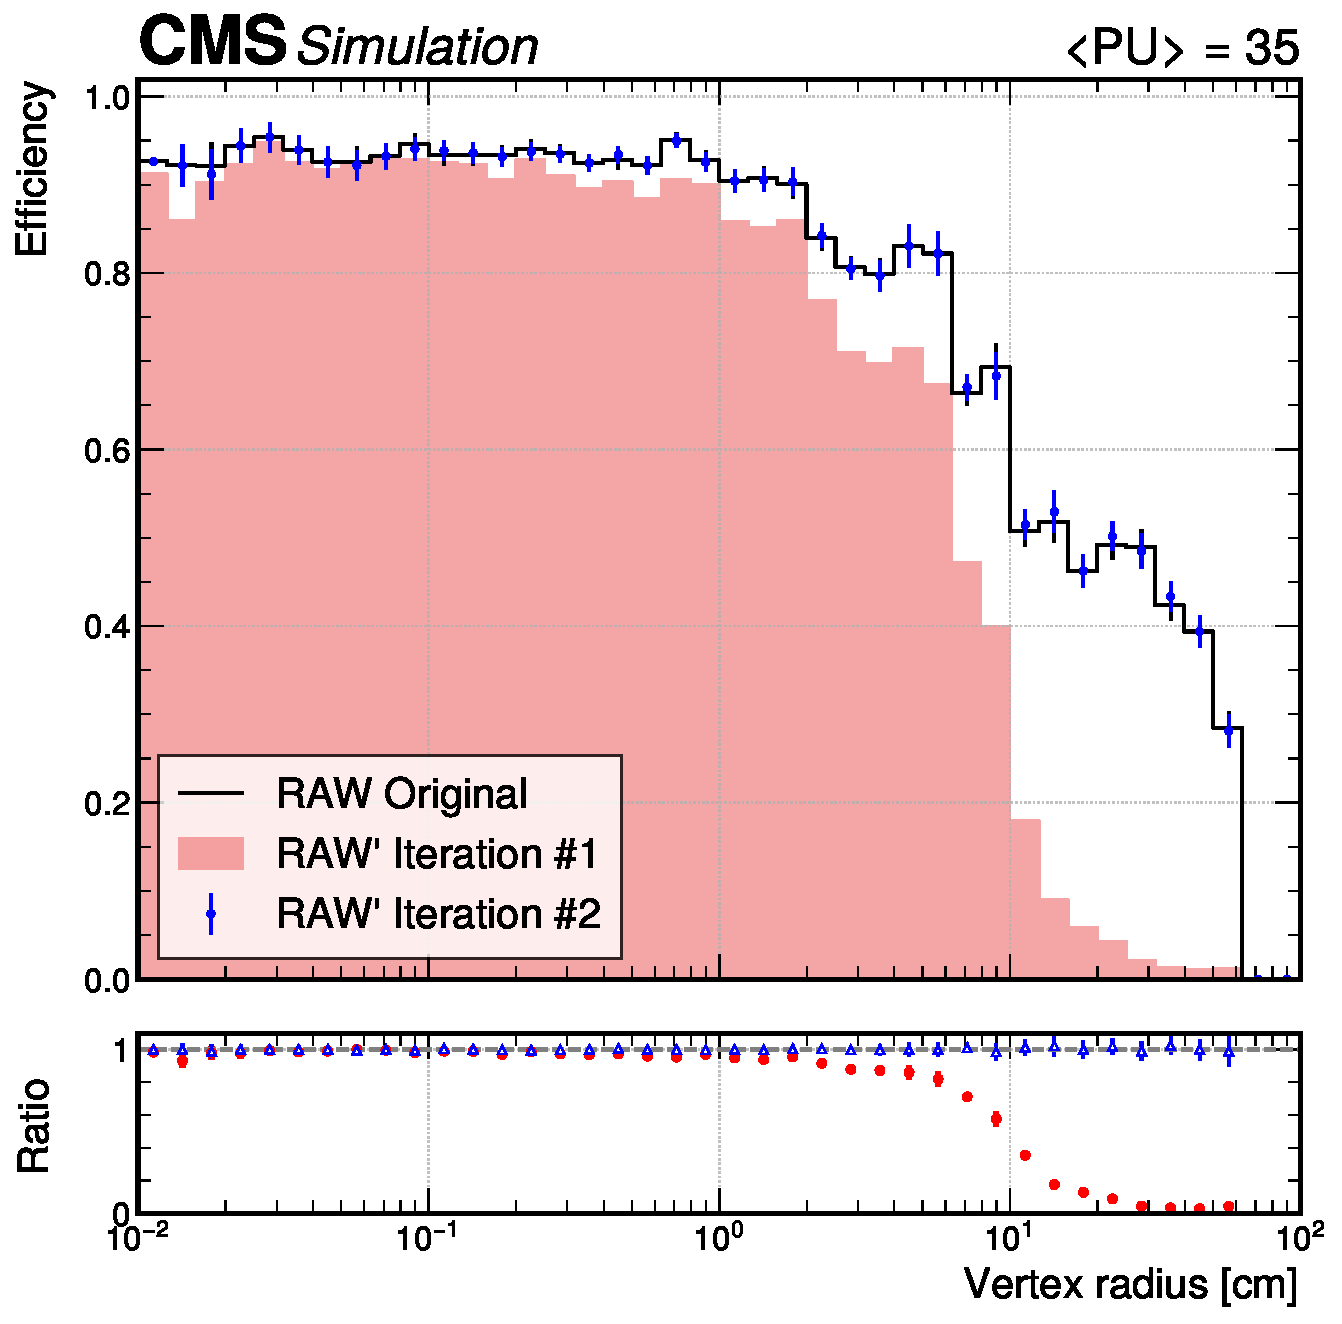
\includegraphics[width=\textwidth]{Figures/Chapter5/efficiency_comparison_2_vertpos.pdf}
            \caption{}
        \end{subfigure}
    \caption[Comparison of the track reconstruction efficiency as a function of $\eta$ and $p_\mathrm{T}$ between the original RAW format, and the alternative RAW' definitions.]{Comparison of the track reconstruction efficiency as a function of \textbf{(a)} $\eta$ and \textbf{(b)} $p_\mathrm{T}$ between the original RAW format, and the alternative RAW' definitions. Results are based on simulated $t\bar{t}$ events.} 
    \label{Figure:Chapter5_TrackingPerformance_2}
\end{figure}

In addition to these global metrics, tracking performance can be further evaluated by
examining the \textit{resolution} of reconstructed quantities such as the IP projections in the transverse plane ($d_{xy}$) and along the beam axis ($d_z$). Comparisons between the different data formats are presented in Figure~\ref{Figure:Chapter5_ResolutionComparison}.

\begin{figure}[h]
        \centering
        % First row
        \begin{subfigure}[b]{0.49\textwidth}
            \centering
            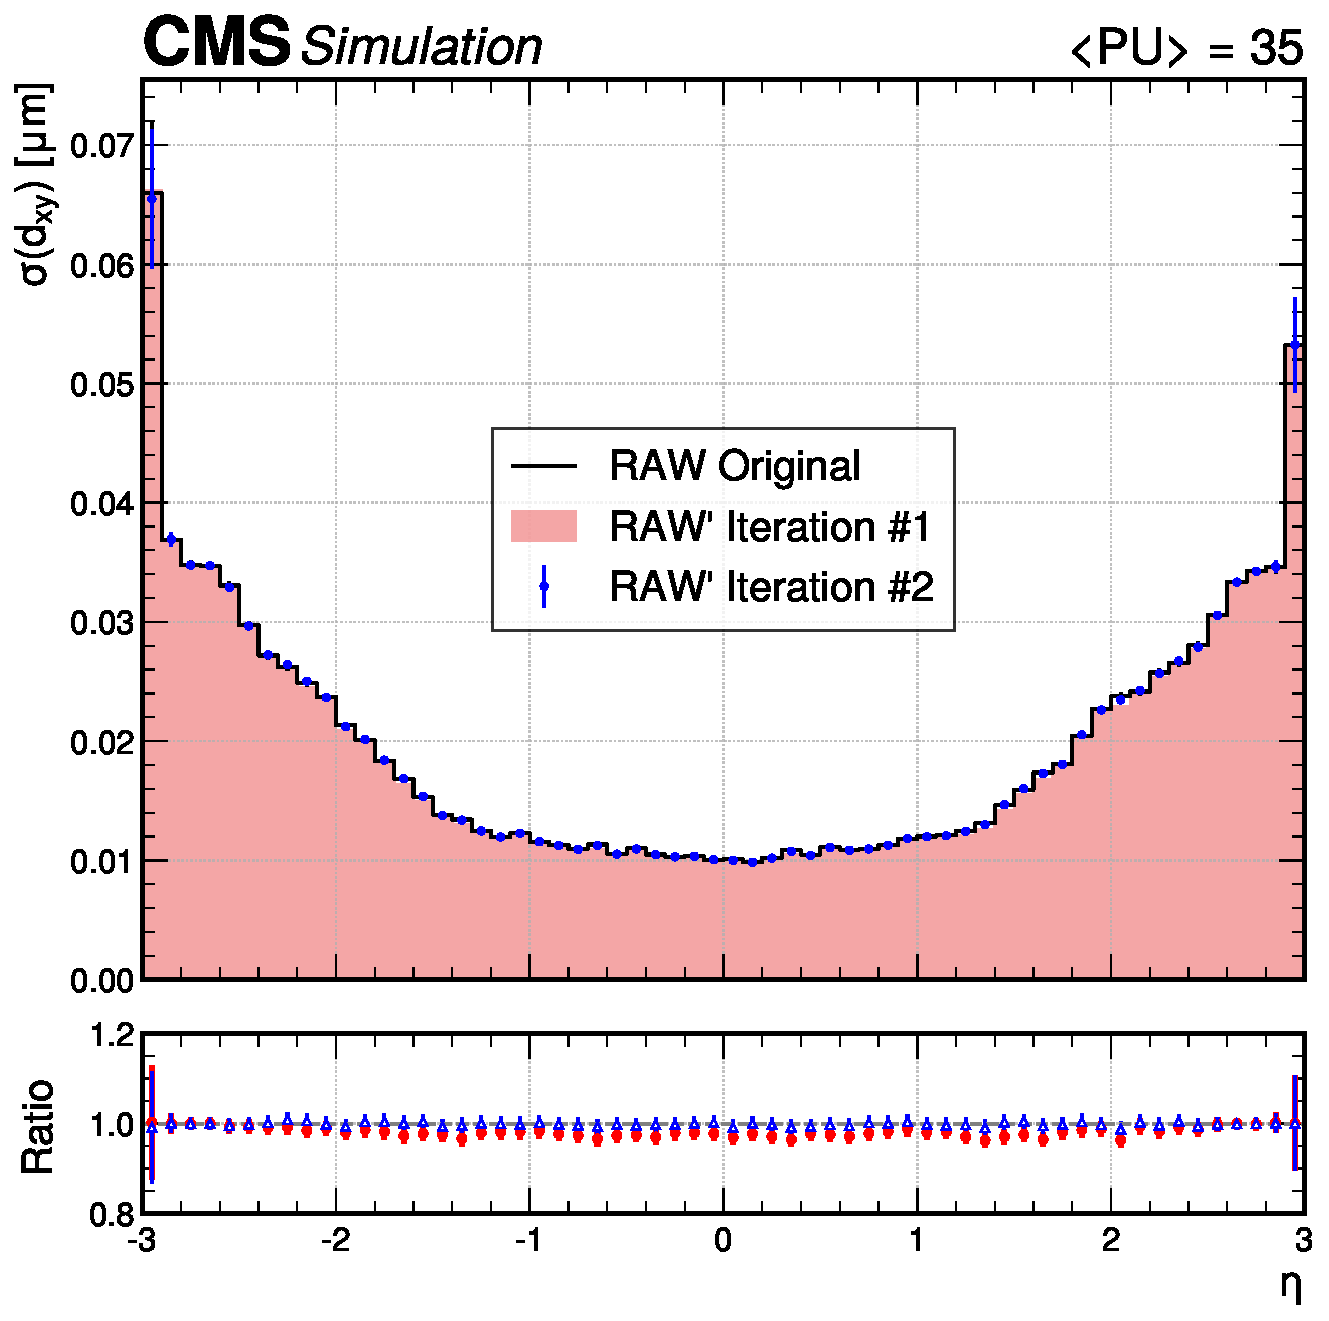
\includegraphics[width=\textwidth]{Figures/Chapter5/resolution_comparison_dxy_eta.pdf}
            \caption{}
        \end{subfigure}
        \begin{subfigure}[b]{0.49\textwidth}
            \centering
            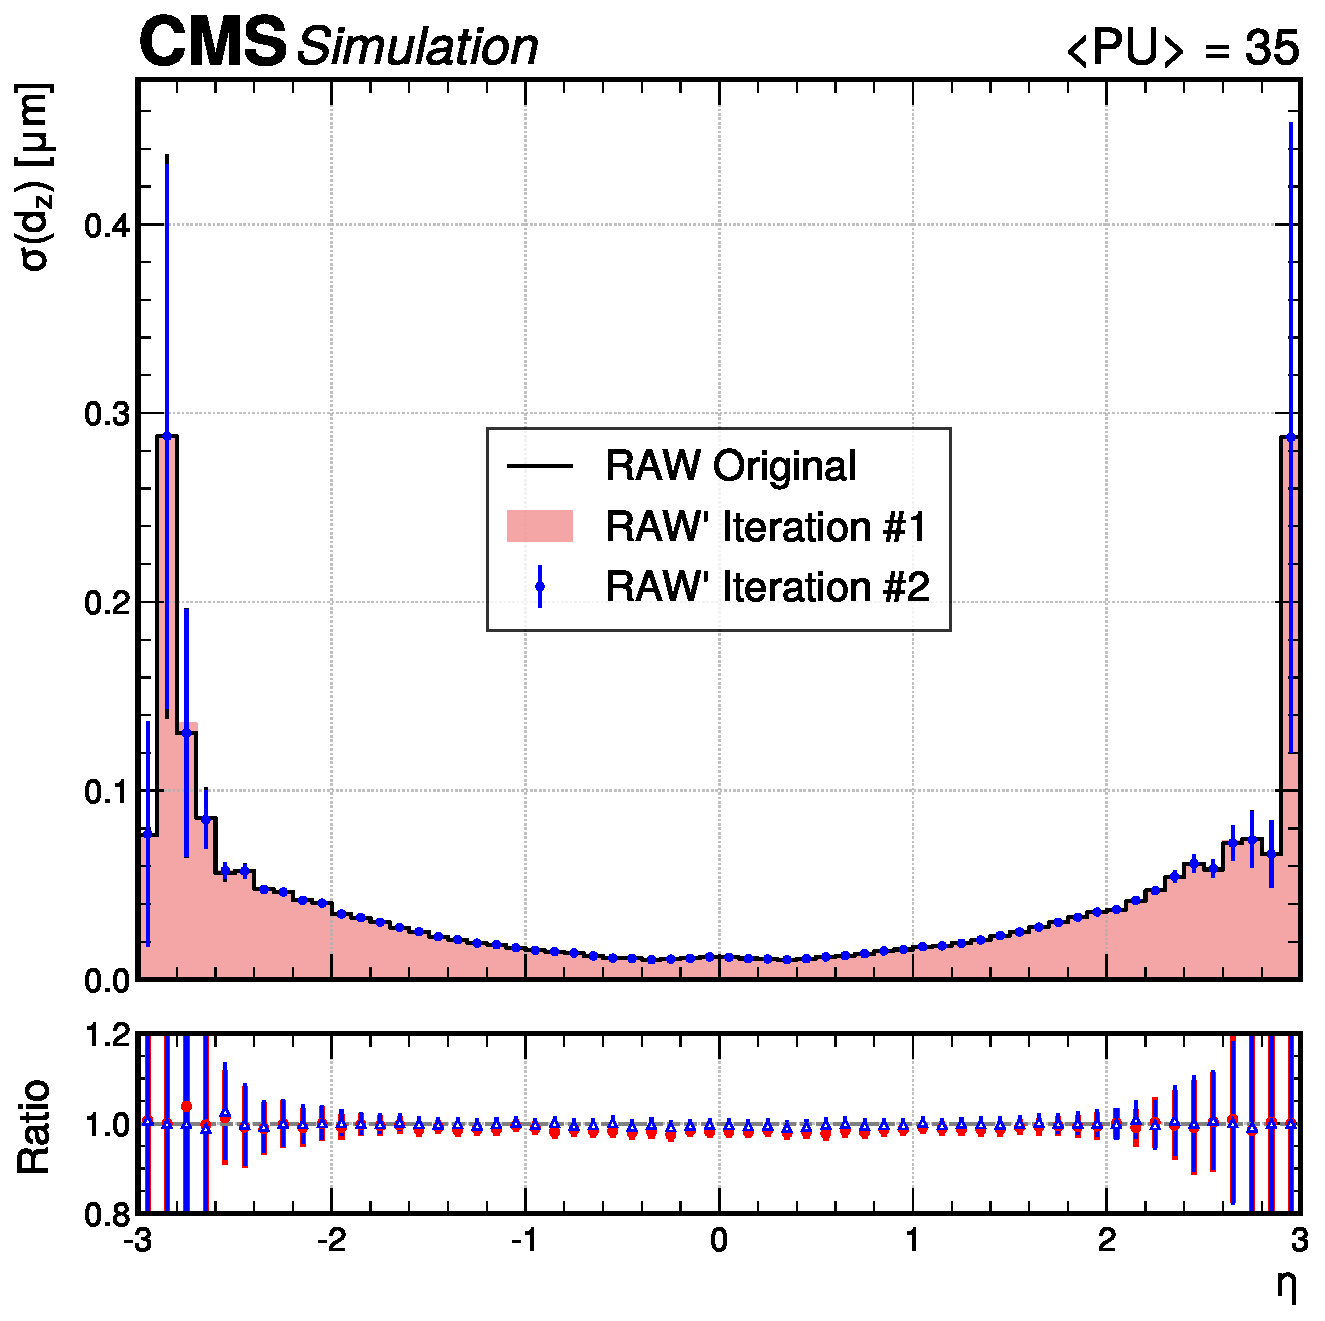
\includegraphics[width=\textwidth]{Figures/Chapter5/resolution_comparison_dz_eta.pdf}
            \caption{}
        \end{subfigure}
        
    \caption[Resolution of IP projections vs $\eta$ for RAW and RAW']{Comparison of the resolution of the \textbf{(a)} transverse and \textbf{(b)} longitudinal impact parameter (IP) projections as a function of $\eta$, comparing the original RAW format to the alternative RAW' definitions. Results are based on simulated $t\bar{t}$ events.}
    \label{Figure:Chapter5_ResolutionComparison}
\end{figure}

While the tracking efficiencies and resolutions achieved with the alternative RAW' format are promising, it is equally important to assess its impact on the reconstruction of long-lived particles with displaced decay signatures, such as the $\mathrm{K}_\mathrm{S}^0$ meson ($c\tau = 2.68\,\unit{cm}$)~\cite{ParticleMasses}. Key performance metrics include the number of reconstructed $\mathrm{K}_\mathrm{S}^0$ candidates and the transverse distance between the particle’s decay point and the primary vertex ($L_{xy}$). As shown in Fig.~\ref{Figure:Chapter5_KsReconstruction}, the updated format exhibits a significant improvement over the first RAW' iteration and achieves performance comparable to the original format. These results further highlight the effectiveness of the enhancements in restoring displaced tracking capabilities.

\begin{figure}[h]
        \centering
        % First row
        \begin{subfigure}[b]{0.49\textwidth}
            \centering
            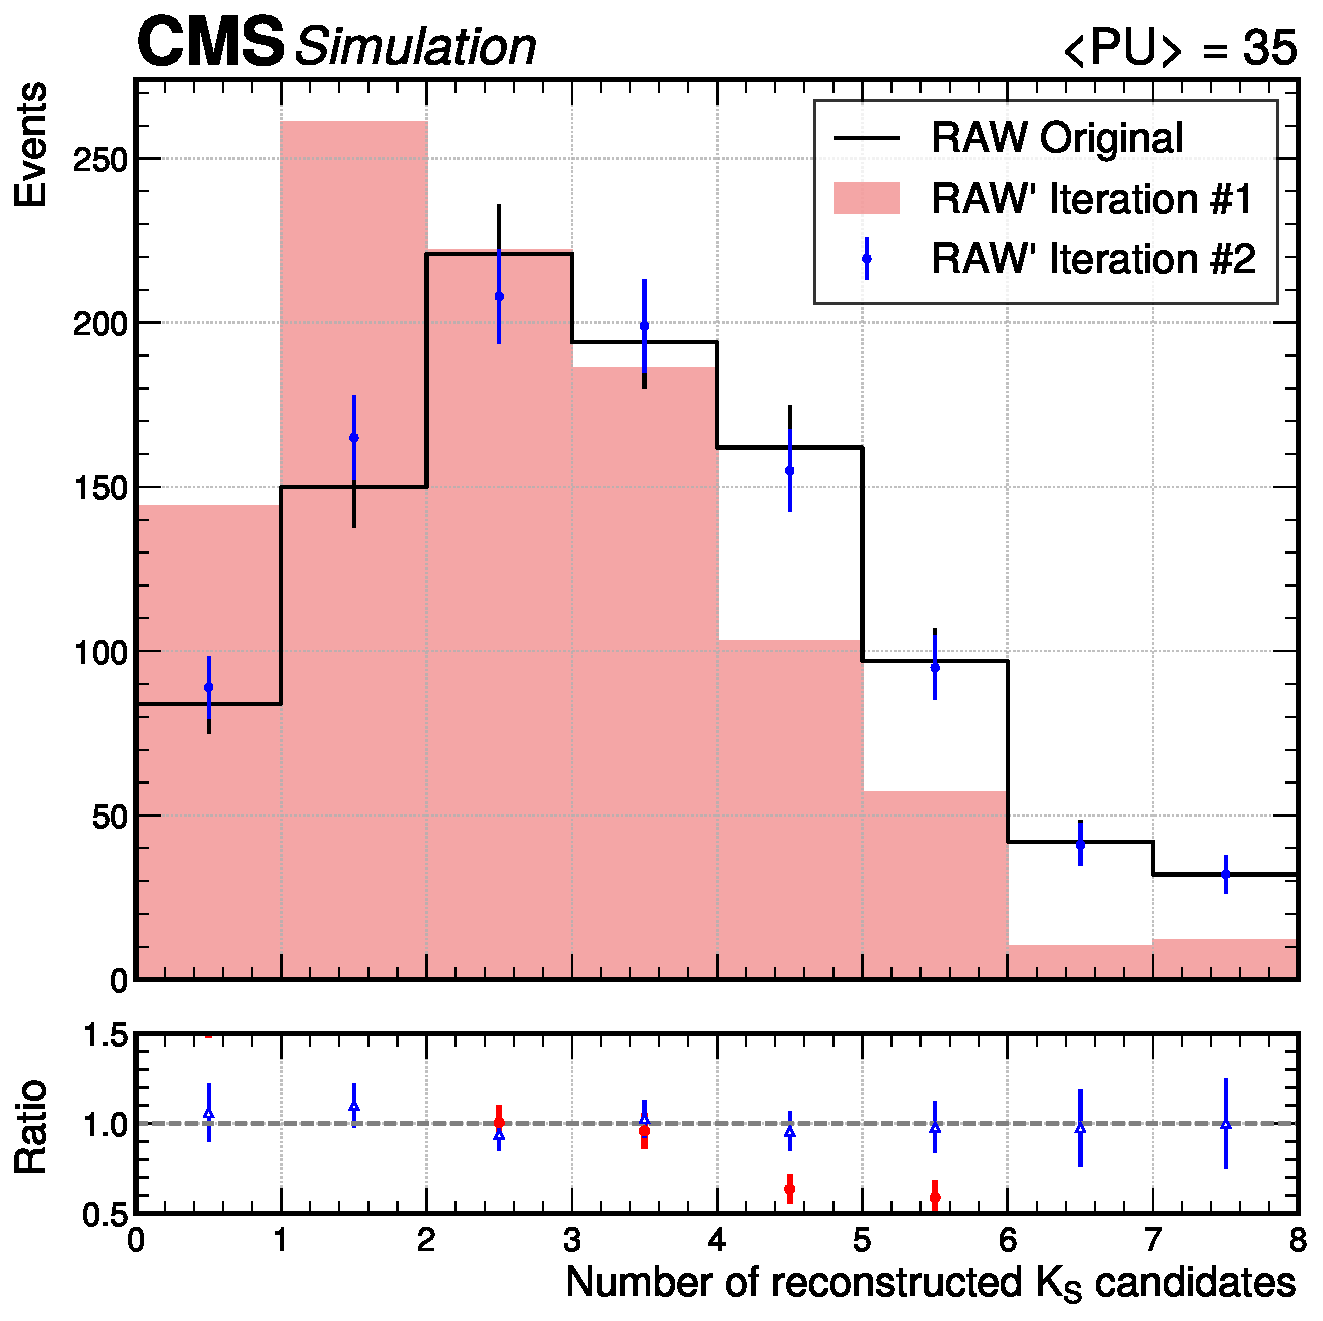
\includegraphics[width=\textwidth]{Figures/Chapter5/Ks_N.pdf}
            \caption{}
        \end{subfigure}
        \begin{subfigure}[b]{0.49\textwidth}
            \centering
            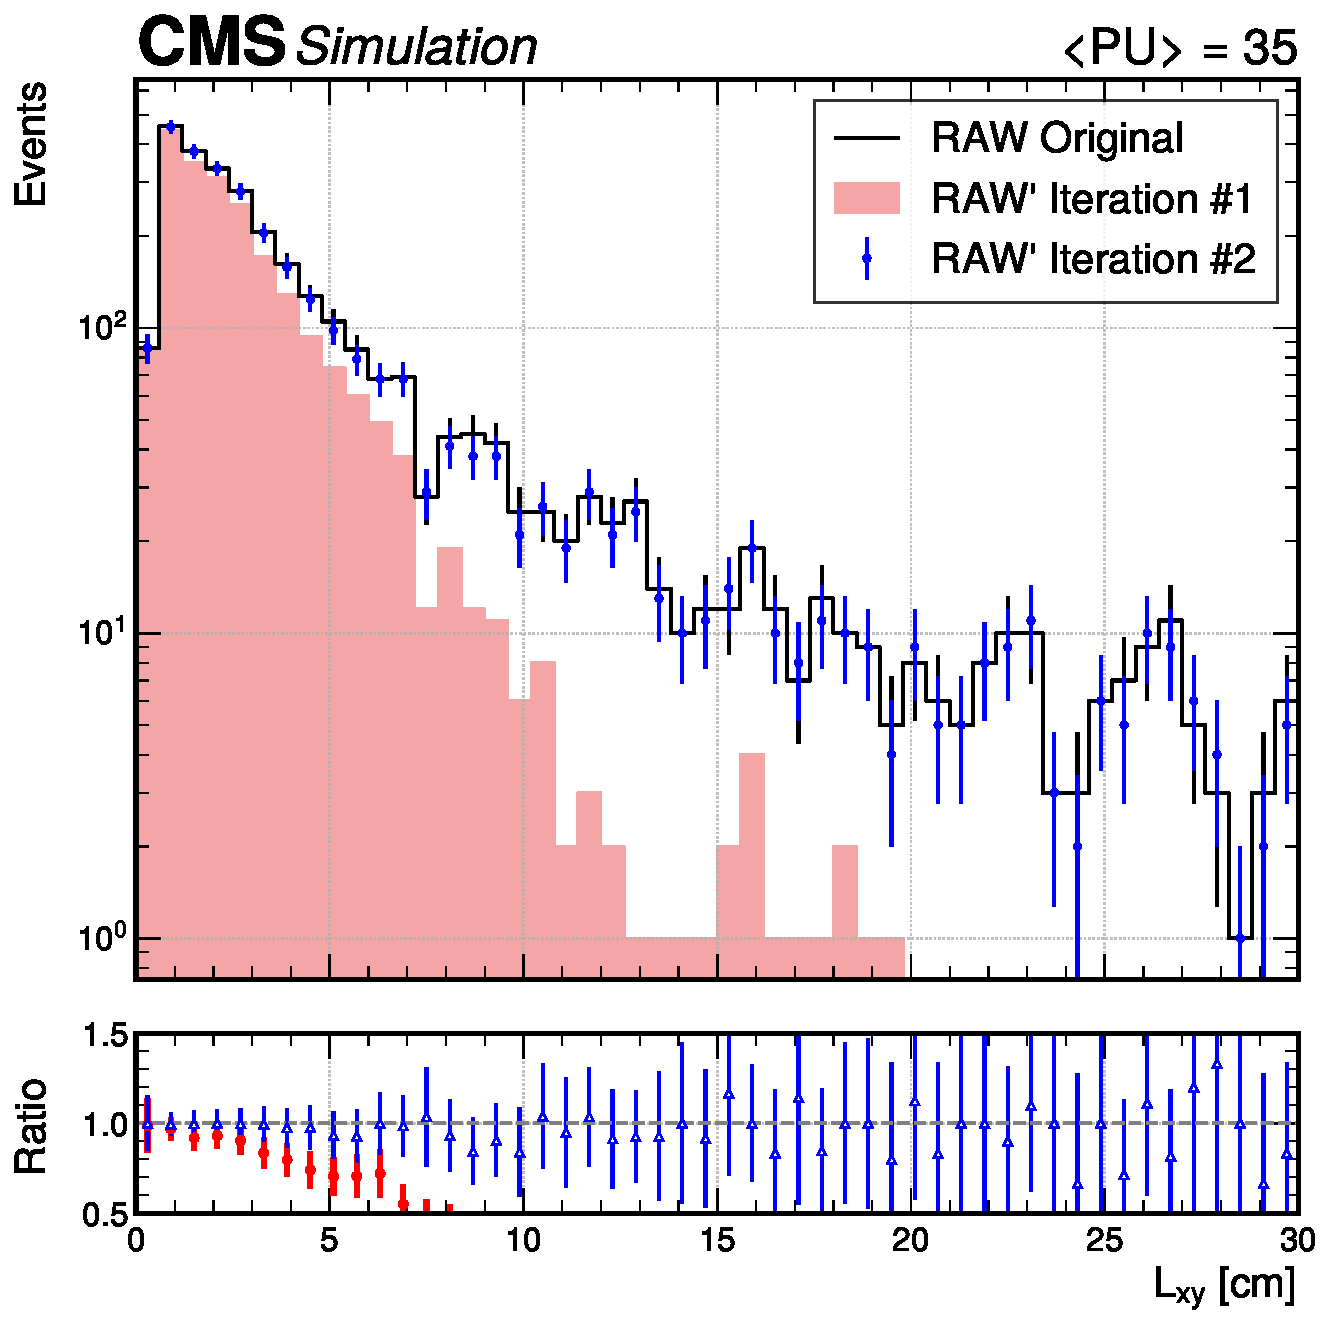
\includegraphics[width=\textwidth]{Figures/Chapter5/Ks_Lxy.pdf}
            \caption{}
        \end{subfigure}

    \caption[Reconstruction of $\mathrm{K}_\mathrm{S}^0$ candidates and $L_{xy}$ for RAW and RAW']{Comparison of the \textbf{(a)} number of reconstructed $\mathrm{K}_\mathrm{S}^0$ candidates and \textbf{(b)} transverse decay length ($L_{xy}$) between the original RAW format and the alternative RAW' definitions. Results are based on simulated $t\bar{t}$ events.}
    \label{Figure:Chapter5_KsReconstruction}
\end{figure}
\setcounter{mtc}{6}
\chapter{\texorpdfstring{Search for extended Higgs sector signatures in $\PGt^+\PGt^-\PGt^+\PGt^-$ final states}{Search for extended Higgs sector signatures in tautautautau final states}}
\chaptermark{Extended Higgs sector search}  
\thispagestyle{plain}  % First page has default style
\pagestyle{chapterpages}
\label{Section:Chapter_4tau}
\minitoc

\section{Introduction}

Motivated by the theoretical considerations and the particularly intriguing measurement of the muon anomalous magnetic moment discussed in Section~\ref{Section:Chapter2_gminus2}, this chapter presents a detailed analysis targeting final states with four tau leptons through the process $Z^*\rightarrow\phi A\rightarrow4\PGt$. The analysis explores a region of parameter space that remains largely unconstrained by existing collider searches. This is primarily because the production mode proceeds via an off-shell $Z^*$ boson. This circumvents the dominant SM Higgs production mechanisms, which are already tightly constrained by current LHC measurements. As such, this search offers unique sensitivity to scenarios in extended Higgs sectors that could otherwise evade detection. This chapter provides a comprehensive description of the analysis strategy employed in the CMS experiment to probe this signature. 

\section{Collision data}

This search is based on pp collision data collected by the CMS detector during the 2016-2018 Run 2 data-taking period. The collisions were recorded at a centre-of-mass energy $\sqrt{s} = 13\TeV$ and the full dataset corresponds to an integrated luminosity of approximately $138\unit{fb}^{-1}$.

\section{Backgrounds}
\label{Section:Chapter6_Backgrounds}
This section provides a brief overview of the SM processes that can contribute to the four-tau signal region. The aim is to provide an understanding of how different backgrounds can enter the selection through the presence of genuine or misidentified tau leptons. The specific treatment of each background category is described in detail in Section~\ref{Section:Chapter6_Background_Modelling}.

The \textbf{\ac{DY}} process, $\PZ/\gamma^* \to \ell^+\ell^-$, is one of the dominant backgrounds in ditau final states, producing genuine $\PGt^+\PGt^-$ pairs in approximately one-third of events. Jets from QCD radiation, specifically from ISR/FSR\footnote{Depending on how the process is generated, ISR/FSR jets may originate from the parton shower or be included at matrix-element level.}, can accompany the boson production. Representative Feynman diagrams illustrating DY production with and without QCD radiation are shown in Fig.~\ref{Figure:Chapter6_DY}. Although its contribution is reduced in this analysis, the DY background remains relevant. Its residual contribution arises through three distinct mechanisms:

\begin{enumerate}[label=(\roman*)]
\item Events with genuine $\PZ/\gamma^* \to \PGt^+\PGt^-$ decays, where accompanying jets are misidentified as $\PGt_h$ candidates.

\item Events with genuine $\PZ/\gamma^* \to e^+e^-$ or $\mu^+\mu^-$ decays, where the prompt electrons or muons are misidentified as leptons from $\PGt$ decays, and accompanying jets are misidentified as $\PGt_h$ candidates.

\item Events with genuine $\PZ/\gamma^* \to e^+e^-$ or $\mu^+\mu^-$ decays, where prompt electrons or muons, as well as accompanying jets, are misidentified as $\PGt_h$ candidates.
\end{enumerate}

\begin{figure}[!htbp]
    \centering
    % First row
    \begin{subfigure}{0.45\textwidth}
        \centering
        \begin{tikzpicture}
    \begin{feynman}
        \vertex at (0, 1.5) (i1) {\(q\)};
        \vertex at (0,-1.5) (i2) {\(\overline{q}\)};

        \vertex at (2,0) (a);
        \vertex at (4, 0) (b);

        \vertex at (6.15, 1.5) (c) {\(\ell^-\)};
        \vertex at (6,-1.5) (d) {\(\ell^+\)};

        \vertex at (3,0.25) () {\(Z/\gamma^*\)};

        \diagram*{
            (i1) -- [fermion] (a) -- [fermion] (i2),
            (a) -- [photon] (b),
            (d) -- [fermion] (b) -- [fermion] (c),
        };
    \end{feynman}
\end{tikzpicture}
        \caption{}
    \end{subfigure}
    \hfill
    \begin{subfigure}{0.45\textwidth}
        \centering
        \begin{tikzpicture}
    \begin{feynman}
        \vertex at (0, 1.5) (i1) {\(q\)};
        \vertex at (0,-1.5) (i2) {\(\overline{q}\)};

        \vertex at (1.35, 0.5) (g1);
        \vertex at (2.5, 1.5) (g2);

        \vertex at (2,0) (a);
        \vertex at (4, 0) (b);

        \vertex at (6.15, 1.5) (c) {\(\ell^-\)};
        \vertex at (6,-1.5) (d) {\(\ell^+\)};

        \vertex at (3,0.25) () {\(Z/\gamma^*\)};

        \diagram*{
            (i1) -- [fermion] (a) -- [fermion] (i2),
            (g1) -- [gluon] (g2),
            (a) -- [photon] (b),
            (d) -- [fermion] (b) -- [fermion] (c),
        };
    \end{feynman}
\end{tikzpicture}
        \caption{}
    \end{subfigure}

    \caption[Examples of Feynman diagrams for Drell-Yan without partons and one parton originating from initial state radiation.]{Examples of Feynman diagrams for Drell-Yan \textbf{(a)} without partons and \textbf{(b)} one parton originating from ISR.}
    \label{Figure:Chapter6_DY}
\end{figure}

\textbf{Diboson} production, specifically $\PZ\PZ \to 4\PGt$, constitutes the primary irreducible background in this analysis. These events contain four genuine $\PGt$ leptons, closely resembling the signal topology by construction. Although the cross section is small compared to other SM processes, their kinematic features make them difficult to distinguish from the signal. Other relevant contributions include $\PZ\PZ \to e^+e^-\PGt^+\PGt^-$ and $\PZ\PZ \to \mu^+\mu^-\PGt^+\PGt^-$, where prompt electrons or muons can be misidentified either as leptons from $\PGt$ decays or as $\PGt_h$ candidates.

\textbf{Top quark pair production} can give rise to events with two genuine $\PGt$ leptons when both $\PW$ bosons decay leptonically to taus. Alternatively, if the $\PW$ bosons decay to electrons or muons, the prompt leptons can be misidentified either as leptonic $\PGt$ decay products or as $\PGt_h$ candidates. A third possibility arises when one or both $\PW$ bosons decay hadronically, producing jets that may be misidentified as $\PGt_h$ candidates. In all cases, the accompanying $b$-jets and additional jets from QCD radiation further contribute to the probability of misreconstruction, resulting in events that appear consistent with a four-tau signature despite containing fewer or no genuine $\PGt$ leptons.

\textbf{W+jets} events can mimic the four-tau topology through mechanisms analogous to those described for top quark pair production, but with only a single $\PW$ boson in the event. Since these events typically contain at most one genuine $\PGt$ lepton, multiple misidentifications are required.

\textbf{QCD-induced multijet} events may satisfy the four-tau selection through multiple misidentification pathways. These events contain no genuine $\PGt$ leptons, but can mimic the signal when several jets are misidentified as $\PGt_h$ candidates. In addition, nonprompt electrons or muons, primarily from semileptonic decays of heavy-flavour hadrons or in-flight decays of light mesons, may be misidentified as leptonic $\PGt$ decays or hadronic $\PGt_h$ candidates.

\textbf{Additional diboson} processes such as $\PW\PW$ and $\PW\PZ$ contribute when one or more of the bosons decay leptonically to taus, producing up to three genuine $\PGt$ leptons. The remaining candidates typically arise from jet or lepton misidentification, as in the DY, $\ttbar$, and W+jets backgrounds.

\textbf{Triboson} production ($\PW\PW\PZ$, $\PZ\PZ\PZ$) can yield three or more prompt leptons, including genuine $\PGt$ decays. These events may include a mix of genuine and misidentified $\PGt$ candidates, analogous to the other backgrounds. Other processes, such as single-top production and electroweak $\PZ/\PW$+jets (\eg VBF-like topologies), contribute via similar mechanisms but are subdominant.

Although many of the backgrounds discussed above are partially reducible through the application of tau identification algorithms, lepton isolation requirements, and $b$-jet vetoes, these techniques are not fully efficient, and some backgrounds remain irreducible. The specific treatment, estimation, and validation of each background category are described in Section~\ref{Section:Chapter6_Background_Modelling}. The simulated background processes used in this analysis are summarised in Table~\ref{Table:Chapter6_SimulatedBackgrounds}.

{
\centering
\setlength{\LTpost}{-2ex}  % tighten space after table
\small  % one size smaller than normal
\begin{longtable}{llc}
\caption[Summary of the simulated Standard Model backgrounds used in the extended Higgs sector search, including their generators and precision.]
{Summary of the simulated SM backgrounds used in this search, including their generators and precision. The following generators were used: 
\MADGRAPH~\cite{MadGraph} for LO matrix element calculations; 
\POWHEG~v1.0~\cite{Powheg_0} and v2.0~\cite{Powheg_1,Powheg_2,Powheg_3} for NLO processes including $\ttbar$ and single top; 
and \MGvATNLO~\cite{MadGraph} for diboson and triboson production. 
Parton showering and hadronisation were performed with \PYTHIA~\cite{PYTHIA}.}
\label{Table:Chapter6_SimulatedBackgrounds} \\
\hline
\textbf{Process} & \textbf{Generators} & \textbf{Cross section $\sigma$ [pb]} \\
\hline \hline
\endfirsthead

\hline
\textbf{Process} & \textbf{Generators} & \textbf{Cross section $\sigma$ [pb]} \\
\hline \hline
\endhead

\hline
\multicolumn{3}{r}{\textit{Continued on next page}} \\
\endfoot

\hline
\endlastfoot
\rowcolor{verylightblue}
\textbf{Drell-Yan, $\PZ/\gamma^* \to \ell^+ \ell^-$ (LO)\hyperlink{DY_W-MLM}{$^1$}} & & \\
+ jets, $10 < m_{\ell \ell} < 50\GeV$ & \MADGRAPH, \PYTHIA & 15810.0 (LO), 18610.0 (NLO) \\
+ jets, $m_{\ell \ell} > 50\GeV$ & \MADGRAPH, \PYTHIA & 5379.0 (LO), 6077.2 (NNLO) \\
+1 jets\hyperlink{DY_W-Stitch}{$^2$}, $m_{\ell \ell} > 50\GeV$ & \MADGRAPH, \PYTHIA & 997.3 (LO) \\
+2 jets\hyperlink{DY_W-Stitch}{$^2$}, $m_{\ell \ell} > 50\GeV$ & \MADGRAPH, \PYTHIA & 347.0 (LO)\\
+3 jets\hyperlink{DY_W-Stitch}{$^2$}, $m_{\ell \ell} > 50\GeV$ & \MADGRAPH, \PYTHIA & 126.4 (LO) \\
+4 jets\hyperlink{DY_W-Stitch}{$^2$}, $m_{\ell \ell} > 50\GeV$ & \MADGRAPH, \PYTHIA & 71.7 (LO) \\

\arrayrulecolor{lightgray}\hline
\rowcolor{verylightblue}
\textbf{W+jets (LO)\hyperlink{DY_W-MLM}{$^1$}} & & \\
+ jets & \MADGRAPH, \PYTHIA & 52940.0 (LO), 61526.7 (NLO) \\
+1 jets\hyperlink{DY_W-Stitch}{$^2$} & \MADGRAPH, \PYTHIA & 9364.4 (LO) \\
+2 jets\hyperlink{DY_W-Stitch}{$^2$} & \MADGRAPH, \PYTHIA & 3168.6 (LO) \\
+3 jets\hyperlink{DY_W-Stitch}{$^2$} & \MADGRAPH, \PYTHIA & 1132.1 (LO) \\
+4 jets\hyperlink{DY_W-Stitch}{$^2$} & \MADGRAPH, \PYTHIA & 633.7 (LO) \\

\arrayrulecolor{lightgray}\hline
\rowcolor{verylightblue}
\textbf{\ttbar} & & \\
Fully hadronic & \POWHEG, \PYTHIA & 377.96 (NNLO)\\
Semi-leptonic & \POWHEG, \PYTHIA & 365.34 (NNLO)\\
Fully leptonic & \POWHEG, \PYTHIA & 88.29 (NNLO) \\

\arrayrulecolor{lightgray}\hline
\rowcolor{verylightblue}
\textbf{Single top} & & \\
t-channel ($t$) & \POWHEG, \PYTHIA & 136.02 (NNLO) \\
t-channel ($\overline{t}$) & \POWHEG, \PYTHIA & 136.02 (NNLO) \\
$t + W^-$ & \POWHEG, \PYTHIA & 35.60 (NNLO) \\
$t + W^+$ & \POWHEG, \PYTHIA & 35.60 (NNLO) \\

\arrayrulecolor{lightgray}\hline
\rowcolor{verylightblue}
\textbf{Diboson} & & \\
$\PW \PZ \rightarrow \ell \, \nu \, \nu \, \nu$  & \MCATNLO, \PYTHIA & 3.416 (NLO) \\
$\PW \PZ \rightarrow \ell \, \nu \, q \, q$        & \MCATNLO, \PYTHIA & 10.71 (NLO) \\
$\PW \PZ \rightarrow q \, q \, \ell \, \ell$            & \MCATNLO, \PYTHIA & 6.419 (NLO) \\
$\PW \PZ \rightarrow \ell \, \ell \,  \ell \, \nu $          & \MCATNLO, \PYTHIA & 5.213 (NLO) \\
$\PW \PW \rightarrow \ell \, \nu \, q \,q$        & \MCATNLO, \PYTHIA & 49.99 (NLO) \\
$\PW \PW \rightarrow \ell \, \nu \, \ell \, \nu$        & \POWHEG, \PYTHIA & 11.09 (NLO) \\
$\PZ \PZ \rightarrow \ell \, \ell \, \nu \, \nu$         & \POWHEG, \PYTHIA & 0.9740 (NLO) \\
\arrayrulecolor{lightgray}\hline
$\text{H}_{\text{VBF}} \rightarrow ZZ \rightarrow \ell \, \ell \, \ell \, \ell $ & \POWHEG, \PYTHIA & $1.040e^{-3}$ (NLO) \\
$\text{ggH} \rightarrow ZZ \rightarrow \ell \, \ell \, \ell \, \ell $ & \POWHEG, \PYTHIA & $1.333e^{-2}$ (NLO)\\
$qq \rightarrow ZZ \rightarrow \ell \, \ell \, \ell \, \ell $ & \POWHEG, \PYTHIA & 1.325 (NLO)\\
$gg \rightarrow ZZ \rightarrow e \, e \, \PGt \, \PGt $ & \PYTHIA & $3.194e^{-3}$ (NLO)\\
$gg \rightarrow ZZ \rightarrow \mu \, \mu \, \PGt \, \PGt $ & \PYTHIA & $3.194e^{-3}$ (NLO)\\
$gg \rightarrow ZZ \rightarrow \mu \, \mu \, \mu \, \mu $ & \PYTHIA & $1.585e^{-3}$ (NLO)\\
$gg \rightarrow ZZ \rightarrow \PGt \, \PGt \, \PGt \, \PGt $ & \PYTHIA & $1.585e^{-3}$ (NLO)\\

\arrayrulecolor{lightgray}\hline
\rowcolor{verylightblue}
\textbf{Triboson} & & \\
$\PW \PW \PZ $ & \MCATNLO, \PYTHIA & 0.1707 (NLO)\\
$\PW \PZ \PZ $ & \MCATNLO, \PYTHIA & 0.0571 (NLO)\\
$\PW \PW \PW $ & \MCATNLO, \PYTHIA & 0.2158 (NLO)\\
$\PZ \PZ \PZ $ & \MCATNLO, \PYTHIA & 0.0148 (NLO)\\

\arrayrulecolor{lightgray}\hline
\rowcolor{verylightblue}
\textbf{Pure Electroweak} & & \\
$\PW^+ \to \ell^+ \nu$ + 2 jets & \MADGRAPH, \PYTHIA & 25.62 (LO)\\
$\PW^- \to \ell^- \nu$ + 2 jets & \MADGRAPH, \PYTHIA & 20.25 (LO)\\
$\PZ \to \ell \ell$ + 2 jets & \MADGRAPH, \PYTHIA & 3.987 (LO)\\

\arrayrulecolor{black}\hline
\end{longtable}
}
\vspace{0.5em}
\noindent\begin{minipage}{\linewidth}
\footnotesize
\hypertarget{DY_W-MLM}{}$^{1}$In the DY+jets simulation, the MLM jet matching scheme~\cite{MLM} is employed to consistently combine partons generated at the matrix-element level with those from the parton shower, avoiding double counting of ISR/FSR jets. \\
\hypertarget{DY_W-Stitch}{}$^{2}$ To improve statistical precision, exclusive samples with fixed jet multiplicities are generated using the MLM scheme. These are stitched with inclusive samples to reproduce the overall cross-section and kinematic distributions accurately.
\end{minipage}

% For \ac{NLO} simulations, however, the MLM scheme is incompatible with the negative event weights that naturally arise. In such cases, the FxFx jet merging scheme~\cite{FxFx} is used instead. 


% Although the background samples are generated at LO or NLO, the comparison of simulated events to data is performed using higher-order theoretical cross-sections. Specifically, $\PW$+jets, Z+jets, $\ttbar$, and single top quark events in the tW channel are normalised using \ac{NNLO} cross-sections~\cite{HighOrder_XS_1,HighOrder_XS_2,HighOrder_XS_3}, while single top and diboson events are normalised to cross-sections calculated at NLO~\cite{HighOrder_XS_3,HighOrder_XS_4,HighOrder_XS_5}.

\section{Modelling of signal processes}
\label{Section:Chapter6_SignalModelling}

Signal templates targeting the process $Z^* \to \phi A \to \PGt^+\PGt^-\PGt^+\PGt^-$ are modelled in the \MCATNLO (version 2.6.5) framework~\cite{MadGraph,FxFx} at NLO accuracy in QCD. Event generation is performed in the five-flavour scheme using the NNPDF3.1 PDFs~\cite{NNPDF}. Parton showering, hadronisation, and $\PGt$ lepton decays are simulated using \PYTHIA (version 8.230)~\cite{PYTHIA}, with the underlying event modelled according to the CP5 tune~\cite{CP5_Tune}. To reflect realistic running conditions, simulated events are overlaid with additional pp interactions according to the PU distribution observed during the Run 2 data-taking period. The detector response is simulated using the \GEANTfour-based CMS software~\cite{GEANT4}, and events are reconstructed with the same configuration as applied to collision data.

A two-dimensional mass grid is defined to ensure sensitivity across the allowed phase space. The grid consists of combinations of $m_A$ and $m_\phi$ as summarised in Table~\ref{Table:Chapter6_4tauMassGrid}.

\begin{table}[!htbp]
\centering
\renewcommand{\arraystretch}{1.5} % Increase row height
\setlength{\tabcolsep}{12pt} % Increase column width
\arrayrulecolor{black} % Ensure outer border is black
\begin{tabular}{cc}
\hline
$m_A$ [GeV] & $m_\phi$ [GeV] \\
\arrayrulecolor{black} \hline

40--90     & 60, 70, 80, 90, 100, 110, 125, 140, 160, 180, 200, 250, 300 \\
\arrayrulecolor{lightgray} \hline

100--250   & 60, 70, 80, 90, 100, 110, 125, 140, 160, 180, 200, 250, 300, 400 \\
\arrayrulecolor{lightgray} \hline

300        & 60, 70, 80, 90, 100, 110, 125, 140, 160, 180, 200, 250, 300, 400, 600 \\
\arrayrulecolor{lightgray} \hline

400        & 100, 110, 125, 140, 160, 180, 200, 250, 300, 400, 600 \\
\arrayrulecolor{lightgray} \hline

600        & 400, 600, 800 \\
\arrayrulecolor{black} \hline

\end{tabular}
\caption{Mass points used in signal generation. For each $m_A$ value, the corresponding $m_\phi$ values are listed.}
\label{Table:Chapter6_4tauMassGrid}
\end{table}

The signal is simulated under the \textit{alignment limit} of the 2HDM, consistent with current experimental constraints on the couplings of the observed Higgs boson. The specific scenario is dynamically selected at each mass point depending on the value of $m_\phi$:
\begin{enumerate}[label=(\roman*)]
    \item For $m_\phi > 125~\GeV$, the heavier CP-even scalar is identified as $\phi \equiv H$
    \item For $m_\phi \leq 125~\GeV$, the lighter CP-even scalar is identified as $\phi \equiv h$
\end{enumerate}

Model parameters such as the charged Higgs mass and the soft $\mathbb{Z}_2$-breaking term have a negligible impact on the kinematic properties of the signal when varied within their allowed ranges. Hence, they are fixed to values that preserve perturbative unitarity, ensuring theoretical consistency~\cite{TypeX_2HDM}. These parameters are set according to the following prescription:

\begin{equation_pad}
m_{H^\pm} = m_\phi, \quad\quad m_{12}^2 = m_\phi^2 \sin\beta \cos\beta.
\end{equation_pad}

Figure~\ref{Figure:Chapter6_GenVisDistributions} illustrates the generator-level distributions of the visible ditau mass ($m_\text{vis}$) for selected combinations of $m_\phi$ and $m_A$. The visible mass is defined as the invariant mass of the visible decay products of the two $\PGt$ leptons, excluding neutrinos. These distributions provide a representative overview of the signal kinematics across the mass grid.

\begin{figure}[!htbp]
        \centering
        % First row
        \begin{subfigure}[b]{0.7\textwidth}
            \centering
            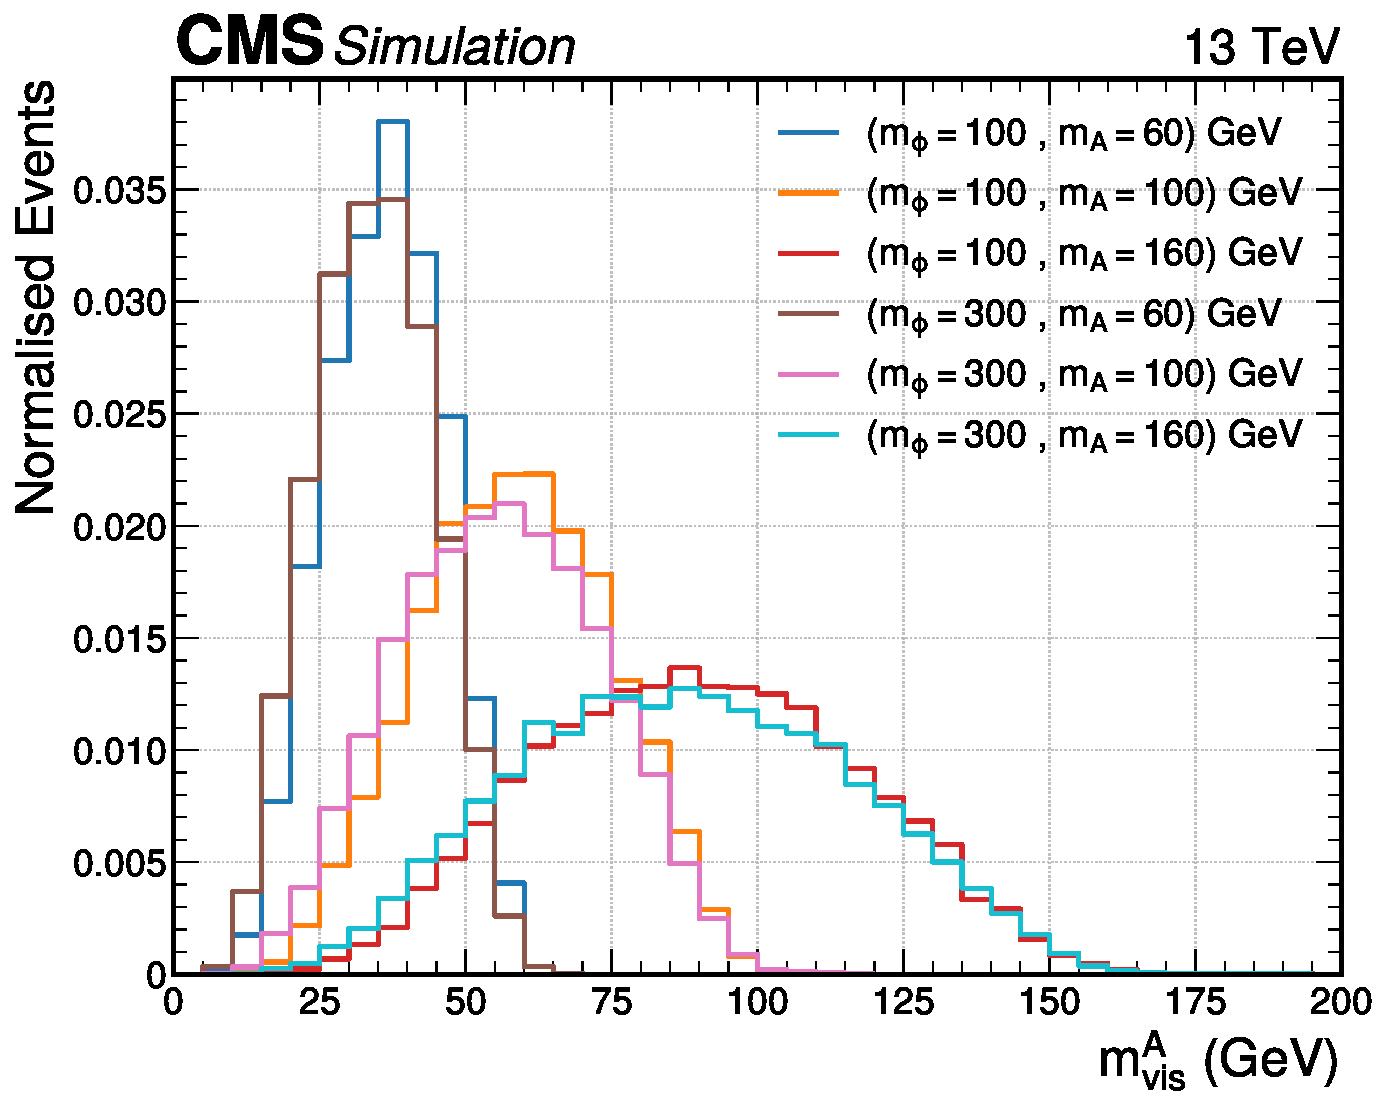
\includegraphics[width=\textwidth]{Figures/Chapter6/mvis_A.pdf}
            \caption{}
        \end{subfigure}
        \hfill
        \begin{subfigure}[b]{0.7\textwidth}
            \centering
            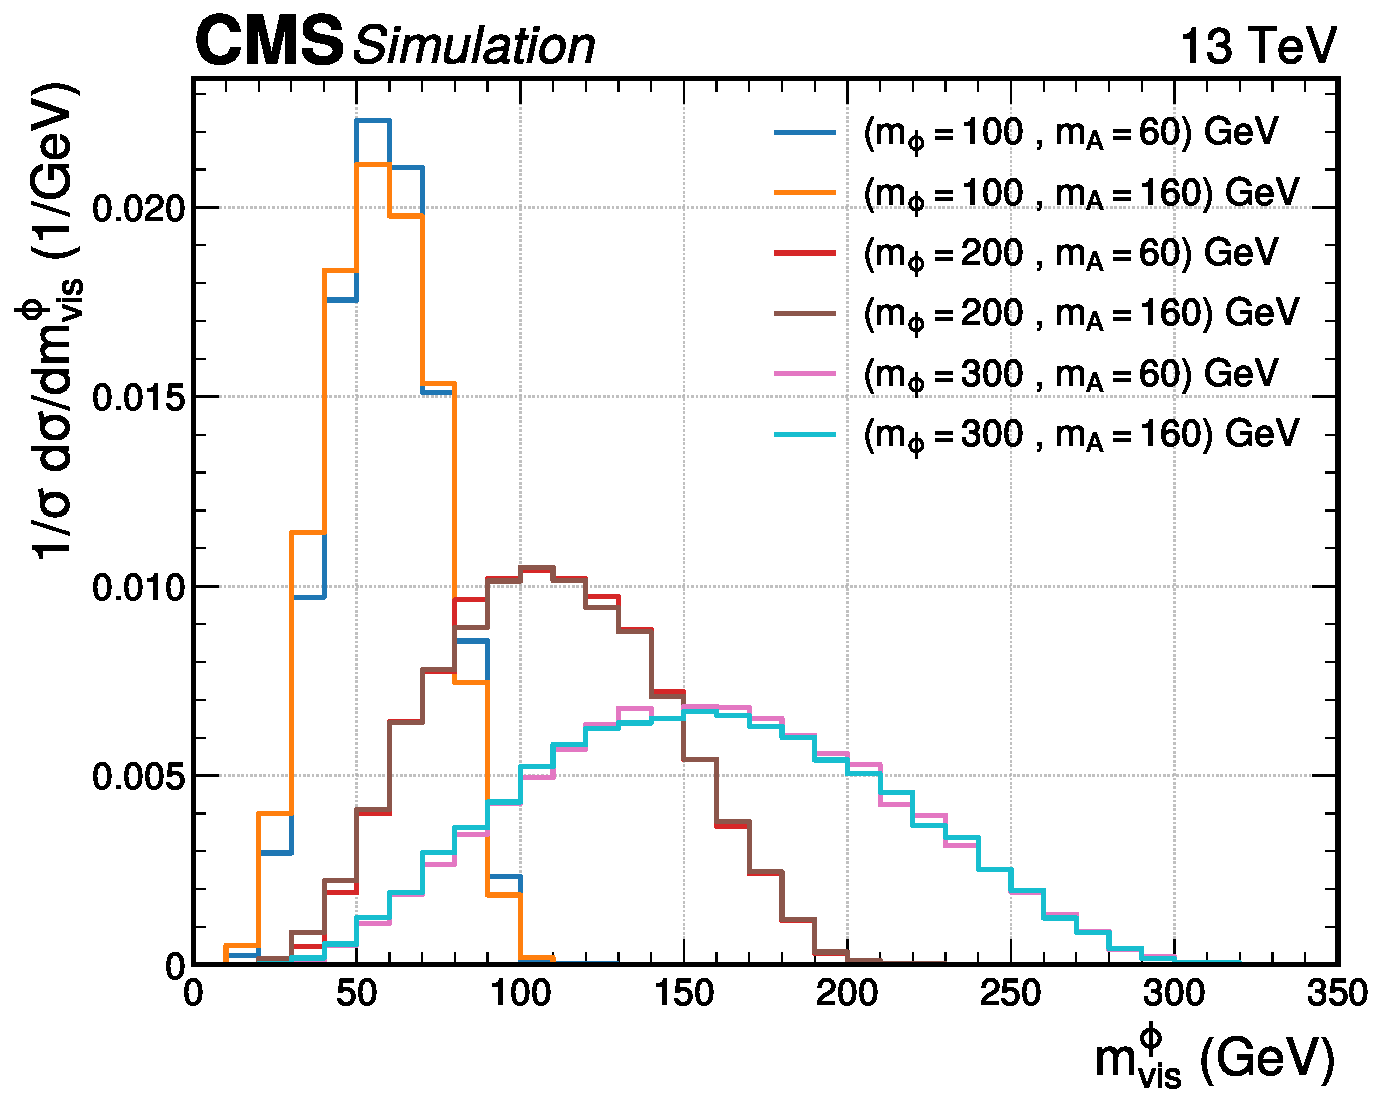
\includegraphics[width=\textwidth]{Figures/Chapter6/mvis_phi.pdf}
            \caption{}
        \end{subfigure}
    \caption[Generator-level visible mass distributions for different mass combinations of $\phi$ and A.]{Generator-level distributions of the visible di-$\PGt$ mass for selected combinations of $m_A$ and $m_\phi$. The visible mass is computed using only the decay products of the two $\PGt$ leptons, excluding neutrinos. Distributions are shown for scans over \textbf{(a)} $m_A$ and \textbf{(b)} $m_\phi$.}
    \label{Figure:Chapter6_GenVisDistributions}
\end{figure}

\subsection{Production cross sections and branching fractions}

The production cross section is computed at NLO in QCD and is independent of $\tan\beta$ within the alignment limit. It varies significantly across the mass plane, ranging from approximately $10~\unit{fb}$ at $(m_\phi, m_A) = (100, 60)~\GeV$ to $650~\unit{fb}$ at $(300, 160)~\GeV$. Figure~\ref{Figure:Chapter6_ProductionXS} summarises these values, showing the cross section as a function of the two mass parameters under the alignment scenario. Outside this limit, the cross section acquires dependence on the scalar mixing angle.

\begin{itemize}
    \item It scales with $\sin^2(\beta - \alpha)$ when $\phi \equiv H$ ($m_\phi > 125~\GeV$),
    \item It scales with $\cos^2(\beta - \alpha)$ when $\phi \equiv h$ ($m_\phi \leq 125~\GeV$).
\end{itemize}

\begin{figure}[!htbp]
  \centering
  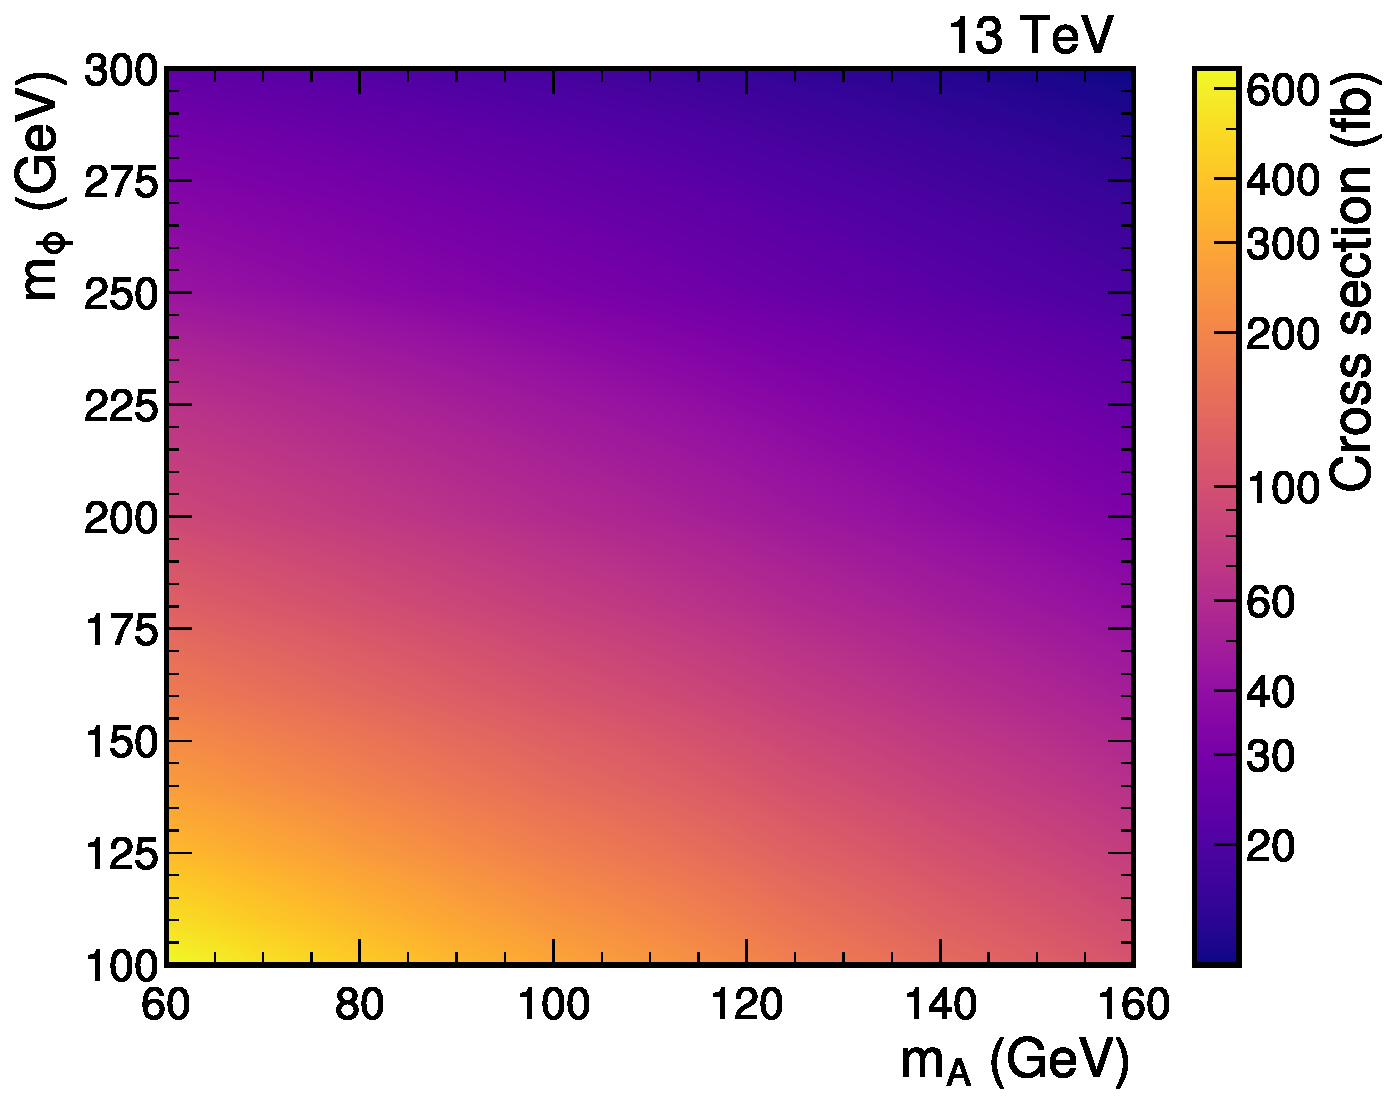
\includegraphics[width=0.7\textwidth]{Figures/Chapter6/Production_XS.pdf}
    \caption[Production cross sections for $Z^* \to \phi A$ in the alignment limit.]{Production cross sections for $Z^* \to \phi A$ in the alignment limit at NLO, shown as a function of $m_\phi$ and $m_A$. The values are interpolated over a grid of simulated mass combinations.}
  \label{Figure:Chapter6_ProductionXS}
\end{figure}

The decay branching fractions of $\phi$ and $A$ into $\PGt^+\PGt^-$ are computed using \textsc{2HDECAY}~\cite{2HDECAY}, a dedicated tool for 2HDM decay widths and branching fractions. In the alignment limit, the $\PGt^+\PGt^-$ branching ratio of $A$ is close to unity for $\tan\beta \gtrsim 2$, but falls sharply at lower values, where hadronic decays such as $A \to b\bar{b}$ become dominant. A similar pattern holds for $\phi \to \PGt^+\PGt^-$, except when the mass difference $m_\phi - m_A$ exceeds $m_Z$. In such cases, the decay $\phi \to ZA$ becomes kinematically accessible and can significantly suppress the ditau branching fraction, even at large $\tan\beta$. These features are illustrated in Figure~\ref{Figure:Chapter6_BranchingFractions}, which shows representative branching fraction maps for selected mass configurations. 

\begin{figure}[!htbp]
        \centering
        % First row
        \begin{subfigure}[b]{0.49\textwidth}
            \centering
            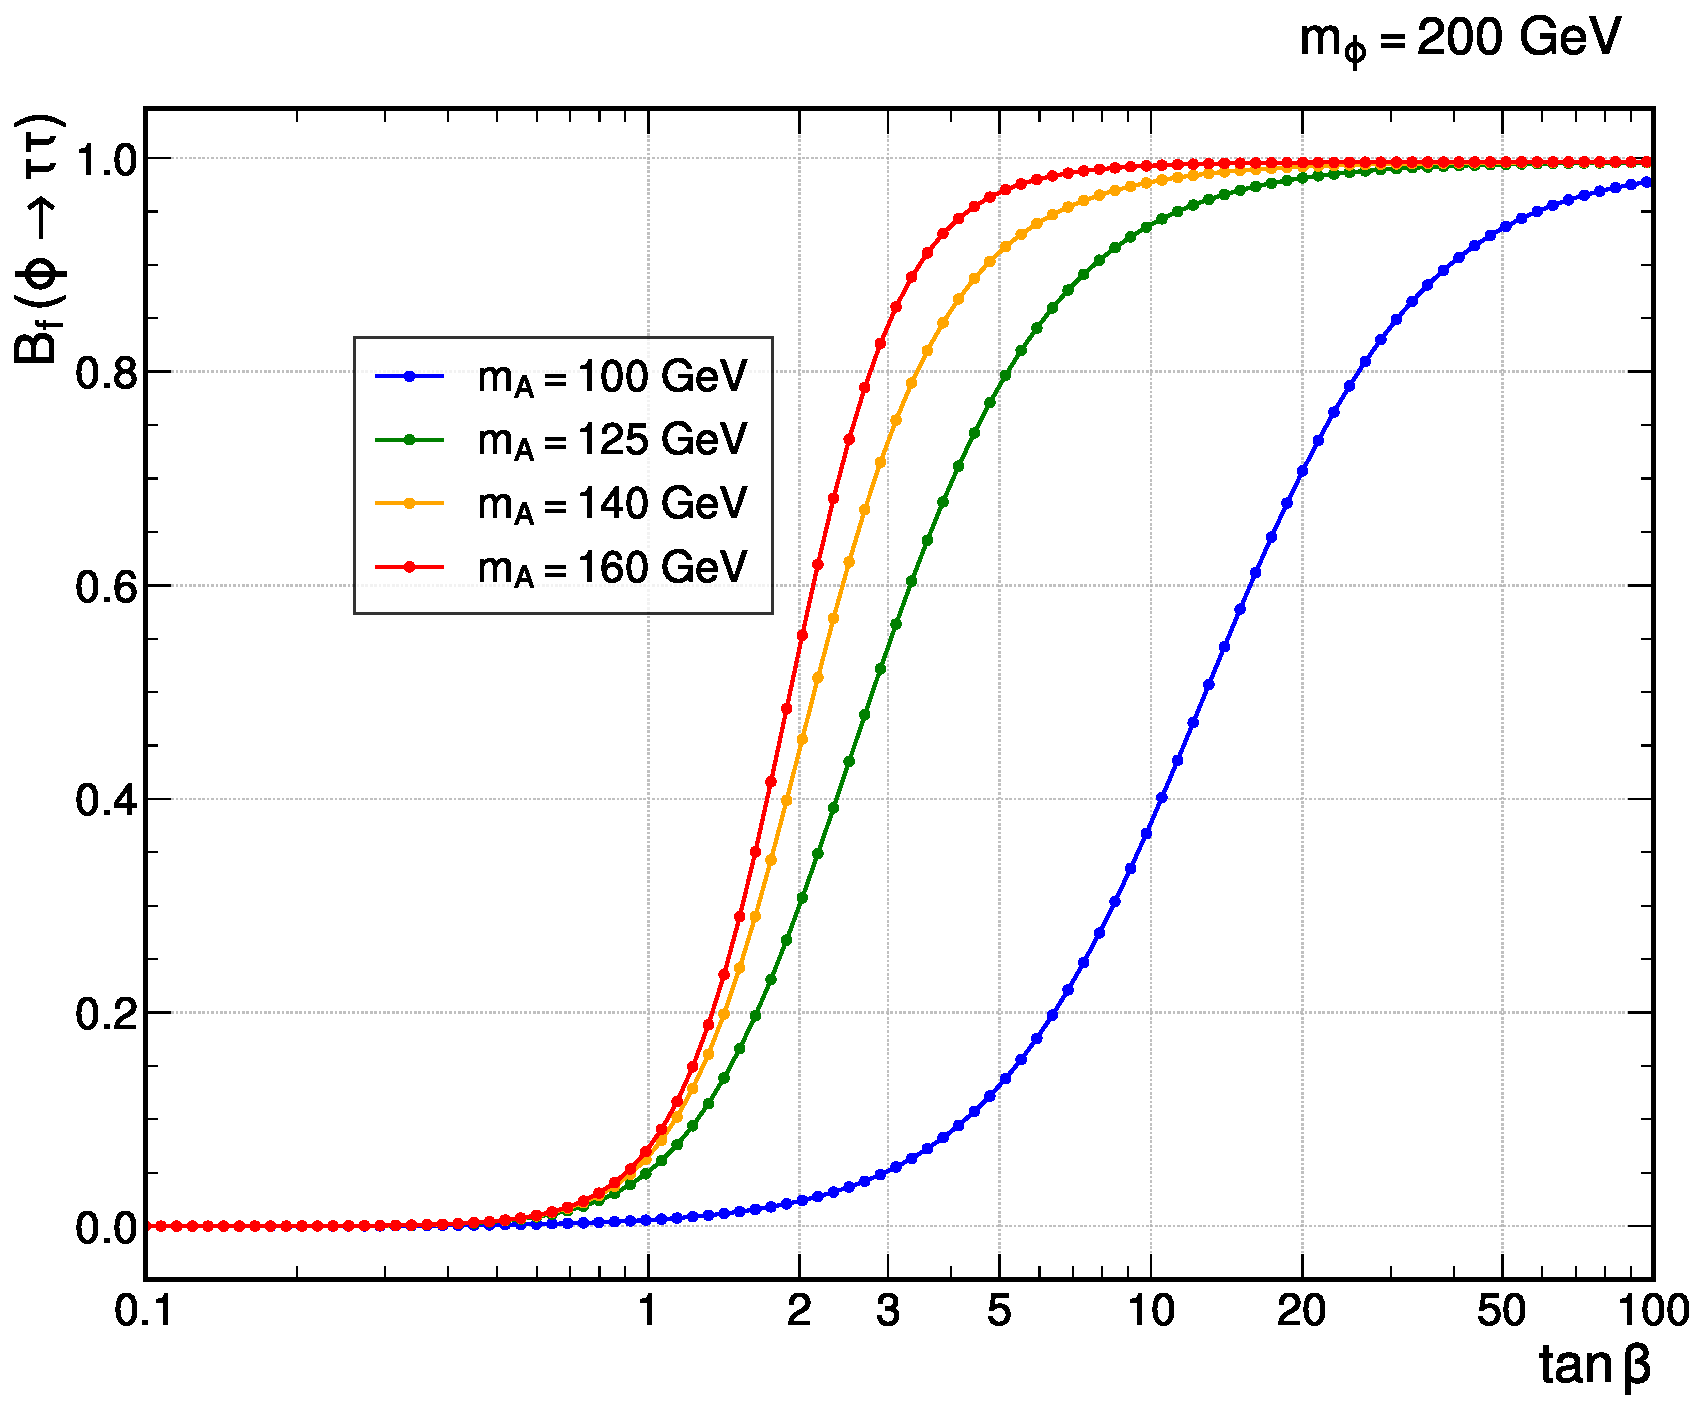
\includegraphics[width=\textwidth]{Figures/Chapter6/Phi_BR.pdf}
            \caption{}
        \end{subfigure}
        \begin{subfigure}[b]{0.49\textwidth}
            \centering
            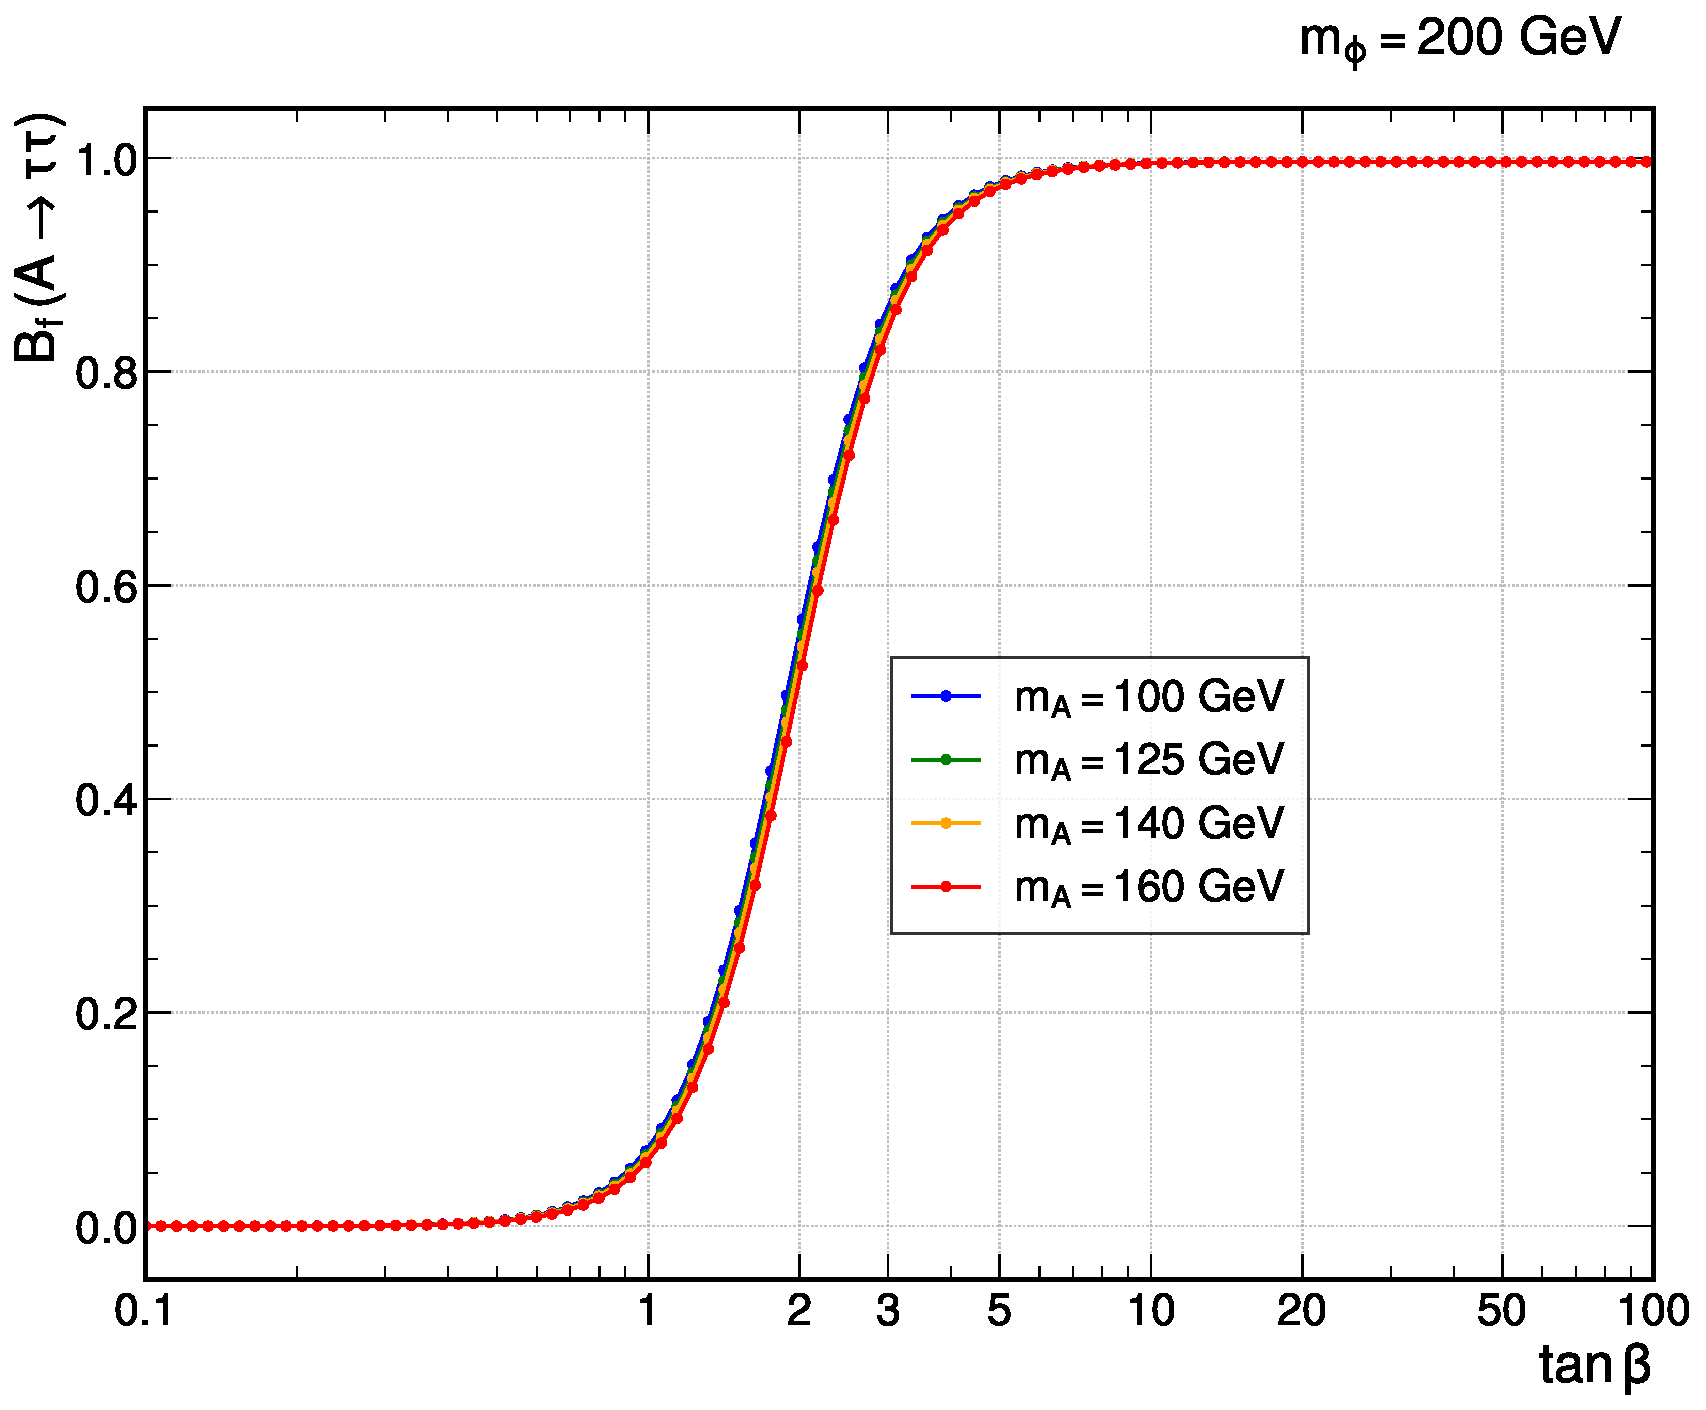
\includegraphics[width=\textwidth]{Figures/Chapter6/A_BR.pdf}
            \caption{}
        \end{subfigure}
    \caption[Branching fractions of $\phi$ and $A$ to $\PGt^+\PGt^-$ for selected mass combinations.]{Branching fractions of \textbf{(a)} $\phi \to \PGt^+\PGt^-$ and \textbf{(b)} $A \to \PGt^+\PGt^-$ as a function of $m_\phi$ and $m_A$, computed using \textsc{2HDECAY} in the alignment limit.}
    \label{Figure:Chapter6_BranchingFractions}
\end{figure}

\section{Event selection strategy}
\label{sec:ObjectAndEventSelections}

The analysis targets $Z^* \to \phi A \to 4\PGt$ decays, where the four taus can produce a wide range of final states depending on their \acp{DM}. Figure~\ref{Figure:Chapter6_4tau_decayModes_BF} shows a pie chart of the most frequent final states, constructed by enumerating all combinations of decay modes and summing their relative branching fractions. Channels containing two or more $\PGt_h$ dominate the total branching fraction, comprising 87.1\% of all decays, and form the primary focus of the analysis. In contrast, Table~\ref{Table:Chapter6_4tau_decayModes_BF_Other} lists rarer final states, which are excluded from the analysis due to their contributions.

\begin{figure}[!htbp]
  \centering
  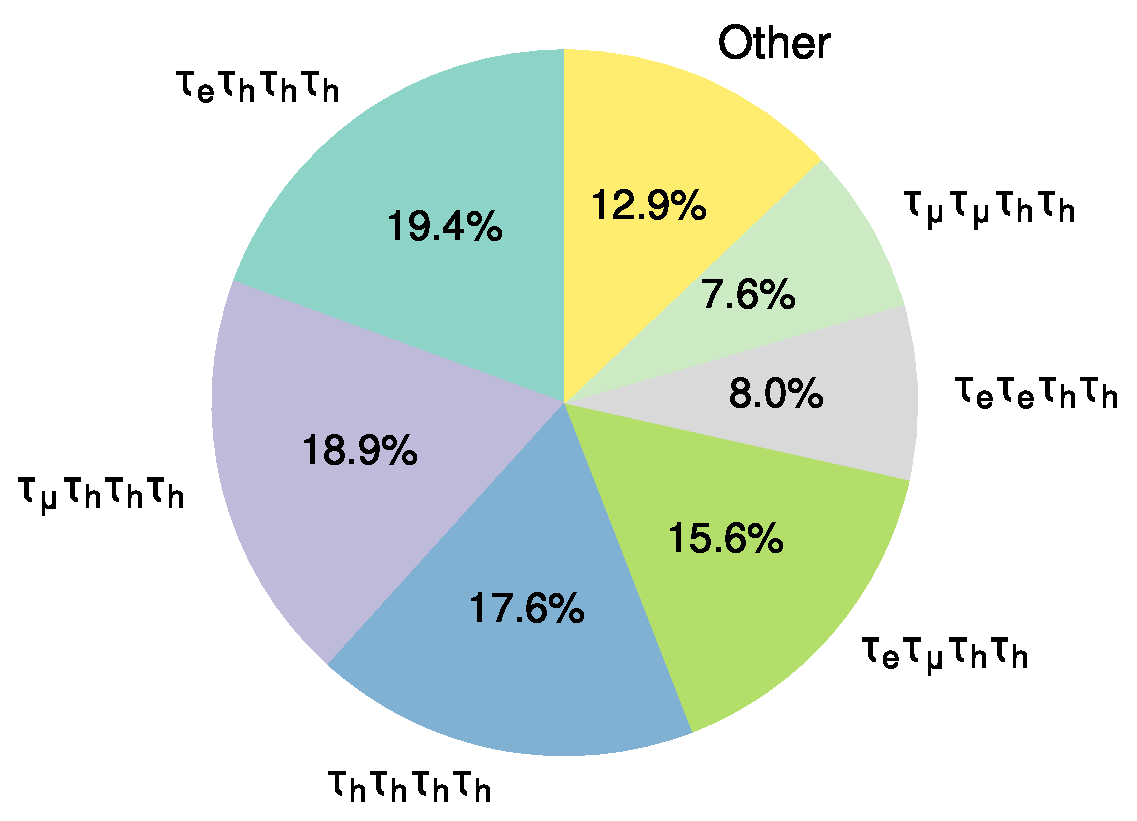
\includegraphics[width=0.9\textwidth]{Figures/Chapter6/pie_BF.pdf}
    \caption[Branching fractions of the dominant four-tau decay modes.]
    {Branching fractions of the most frequent four-tau final states, constructed by enumerating all combinations of tau decays.}
  \label{Figure:Chapter6_4tau_decayModes_BF}
\end{figure}

\begin{table}[!htbp]
\centering
\renewcommand{\arraystretch}{1.5} % Increase row height
\setlength{\tabcolsep}{12pt} % Increase column width
\arrayrulecolor{black} % Ensure outer border is black
\begin{tabular}{cc}
\hline
Decay Mode                  & Branching Fraction {[}\%{]} \\ \hline 
$\PGt_e \PGt_e \PGt_{\mu} \PGt_h$             & 4.3 \\ 
\arrayrulecolor{lightgray} \hline
$\PGt_e \PGt_{\mu} \PGt_{\mu} \PGt_h$                    & 4.2 \\ 
\arrayrulecolor{lightgray} \hline
$\PGt_e \PGt_e \PGt_{e} \PGt_h$                        & 1.5  \\ 
\arrayrulecolor{lightgray} \hline
$\PGt_{\mu} \PGt_{\mu} \PGt_{\mu} \PGt_h$                  & 1.4  \\ 
\arrayrulecolor{lightgray} \hline
$\PGt_e \PGt_e \PGt_{\mu} \PGt_{\mu}$             & 0.6  \\ 
\arrayrulecolor{lightgray} \hline
$\PGt_e \PGt_e \PGt_{e} \PGt_{\mu}$                     & 0.4  \\ 
\arrayrulecolor{lightgray} \hline
$\PGt_e \PGt_{\mu} \PGt_{\mu} \PGt_{\mu}$             & 0.4  \\ 
\arrayrulecolor{lightgray} \hline
$\PGt_e \PGt_e \PGt_{e} \PGt_e$                  & 0.1  \\ 
\arrayrulecolor{lightgray} \hline
$\PGt_{\mu} \PGt_{\mu} \PGt_{\mu} \PGt_{\mu}$                  & 0.1  \\ 
\arrayrulecolor{black} \hline
\end{tabular}
\caption[Branching fractions of subdominant four-tau decay modes]{Branching fractions of subdominant four-tau final states, involving three or more leptonic $\PGt$ decays.}
\label{Table:Chapter6_4tau_decayModes_BF_Other}
\end{table}

To improve acceptance for events in which one $\PGt_h$ candidate fails to be reconstructed, an orthogonal $\PGt_h\PGt_h\PGt_h$ channel is also included. This typically captures partially reconstructed $\PGt_h\PGt_h\PGt_h\PGt_h$ decays where one candidate fails trigger or identification requirements, often due to high $p_\text{T}$ thresholds or limited efficiency. In total, seven signal regions are defined. Additionally, a control region based on the fully leptonic $\PGt_{\mu} \PGt_{\mu} \PGt_{\mu} \PGt_{\mu}$ final state is used to constrain the modelling of backgrounds composed entirely of genuine leptons, as discussed in Section~\ref{Section:Chapter6_Background_Modelling}.

\subsection{Triggering}

Identifying events with this topology presents a unique challenge, as no dedicated trigger exists. Instead, the selection strategy relies on a combination of standard single- and multi-object triggers that are sensitive to subsets of the final-state decay products. These include single-lepton (electron or muon), double-electron, double-muon, and double-tau triggers. Cross-triggers, such as those combining a lepton and a hadronic tau ($e+\tau_h$, $\mu+\tau_h$) or the electron–muon trigger, were also considered. However, they provide negligible gains in signal acceptance and are excluded. Although single-$\tau_h$ triggers are also available, their high $p_\text{T}$ thresholds are too restrictive for the phase space relevant to this search. The triggers used in the analysis, along with the corresponding online $p_\text{T}$ thresholds for each data-taking year, are summarised in Table~\ref{Table:Chapter6_TriggerThresholdsExpanded}.

\begin{table}[!htbp]
\centering
\renewcommand{\arraystretch}{1.5}
\setlength{\tabcolsep}{12pt} % Increase column width
\begin{tabular}{|c|cc|cc|cc|}
\hline
\multirow{3}{*}{\text{Trigger}} 
& \multicolumn{6}{c|}{$p_\text{T}$ \text{Threshold (GeV)}} \\ \cline{2-7}
& \multicolumn{2}{c|}{\text{2016}} & \multicolumn{2}{c|}{\text{2017}} & \multicolumn{2}{c|}{\text{2018}} \\ \cline{2-7}
& \text{Obj$_1$} & \text{Obj$_2$} & \text{Obj$_1$} & \text{Obj$_2$} & \text{Obj$_1$} & \text{Obj$_2$} \\ \hline \hline
Single-Electron (e)                   & 26     & --     & 28     & --     & 33     & --     \\
\arrayrulecolor{lightgray} \hline
Single-Muon ($\mu$)                       & 23     & --     & 25     & --     & 25     & --     \\
\arrayrulecolor{lightgray} \hline
Double-Tau ($\PGt \PGt$)         & 40     & 40     & 40     & 40     & 40     & 40     \\
\arrayrulecolor{black} \hline
\end{tabular}
\caption{Table of minimum online $p_\text{T}$ thresholds for the triggers used in the analysis. Subcolumns refer to thresholds for the first and second trigger objects.}
\label{Table:Chapter6_TriggerThresholdsExpanded}
\end{table}

The trigger configuration applied to each channel is summarised in Table~\ref{Table:Chapter6_TriggersPerChannel}. A trigger is considered to have fired for a given event if any of the listed object combinations satisfy the corresponding online requirements. The logical OR operator ($\lor$) denotes the inclusive selection, corresponding to the union of all trigger paths associated with that channel.

\begin{table}[!htbp]
\centering
\renewcommand{\arraystretch}{1.5}
\setlength{\tabcolsep}{12pt}
\begin{tabular}{cc}
\hline
Channel & Trigger Configuration \\ \hline 

$\tau_h\tau_h\tau_h\tau_h$ &  
$\tau_1\tau_2 \mathbin{\lor} \tau_1\tau_3 \mathbin{\lor} \tau_1\tau_4 \mathbin{\lor} \tau_2\tau_3 \mathbin{\lor} \tau_2\tau_4 \mathbin{\lor} \tau_3\tau_4$ \\ 
\arrayrulecolor{lightgray} \hline

$\tau_h\tau_h\tau_h$ &
$\tau_1\tau_2 \mathbin{\lor} \tau_1\tau_3 \mathbin{\lor} \tau_2\tau_3$ \\
\arrayrulecolor{lightgray} \hline

$\tau_e\tau_h\tau_h\tau_h$ &
$e_1 \mathbin{\lor} \tau_2\tau_3 \mathbin{\lor} \tau_2\tau_4 \mathbin{\lor} \tau_3\tau_4$ \\
\arrayrulecolor{lightgray} \hline

$\tau_\mu\tau_h\tau_h\tau_h$ &
$\mu_1 \mathbin{\lor} \tau_2\tau_3 \mathbin{\lor} \tau_2\tau_4 \mathbin{\lor} \tau_3\tau_4$ \\
\arrayrulecolor{lightgray} \hline

$\tau_e\tau_e\tau_h\tau_h$ &
$e_1 \mathbin{\lor} e_2 \mathbin{\lor} \tau_3\tau_4$ \\
\arrayrulecolor{lightgray} \hline

$\tau_\mu\tau_\mu\tau_h\tau_h$ &
$\mu_1 \mathbin{\lor} \mu_2 \mathbin{\lor} \tau_3\tau_4$ \\
\arrayrulecolor{lightgray} \hline

$\tau_e\tau_\mu\tau_h\tau_h$ &
$e_1 \mathbin{\lor} \mu_1 \mathbin{\lor} \tau_3\tau_4$ \\
\arrayrulecolor{lightgray} \hline

$\tau_\mu \tau_\mu \tau_\mu \tau_\mu$ &
$\mu_1 \mathbin{\lor} \mu_2 \mathbin{\lor} \mu_3 \mathbin{\lor} \mu_4$ \\
\arrayrulecolor{black} \hline

\end{tabular}
\caption[Trigger configuration used for each four-tau final state.]{Trigger configuration used for each four-tau final state. The labels $e_i$, $\mu_i$, and $\tau_i$ denote individual trigger objects corresponding to electrons, muons, and hadronic taus, respectively, with index $i$ indicating the ordering of candidates in the event.}
\label{Table:Chapter6_TriggersPerChannel}
\end{table}

\subsection{Offline object selections}
\label{Section:Chapter6_ObjectSelection}

Offline selection criteria are applied to reconstructed electrons, muons, and $\PGt_h$candidates, as introduced in Chapter~\ref{Section:Chapter4}. These selections suppress backgrounds from nonprompt and misidentified particles while maintaining high signal efficiency. To ensure consistency with the PV and reduce contamination from PU, all selected objects are required to originate from the PV. This is enforced through cuts on transverse and longitudinal impact parameters: $|d_{xy}| < 0.045\unit{cm}$ and $|d_z| < 0.2\unit{cm}$ for electrons and muons, and $|d_z| < 0.2\unit{cm}$ for $\PGt_h$ candidates.

Electrons and muons are further required to be isolated from surrounding hadronic activity. The relative isolation variables used are defined in Chapter~\ref{Section:Chapter4}, Equations~\ref{Equation:Chapter4_PFIso_Electron} and~\ref{Equation:Chapter4_PFIso_Muon}, with a threshold of $I^{e/\mu}_\text{PF} < 0.15$. No explicit isolation cut is applied to hadronic tau candidates, as this information is embedded in the DeepTau discriminators.

Identification criteria follow those detailed in Sections~\ref{Section:Electron_Identification},~\ref{Section:Muon_Identification}, and~\ref{Section:Chapter4_Taus}. Electrons are selected using a BDT-based discriminator targeting 90\% efficiency, with isolation variables excluded from the training. Muons are required to pass the cut-based medium working point. For $\PGt_h$ candidates, a looser identification is applied to retain adequate signal yields. Candidates must pass the Loose working point of the $D_{\text{jet}}$ discriminator, along with misidentified-lepton rejection cuts: VVLoose for $D_e$ and VLoose for $D_\mu$. 

To ensure consistency between trigger and offline reconstruction, selected objects must match the corresponding trigger-level objects within a cone of $\Delta R < 0.5$. The number of required matches depends on the trigger configuration for each channel, as outlined in Table~\ref{Table:Chapter6_TriggersPerChannel}. For channels using double-object triggers (\eg $\tauh\tauh\tauh\tauh$), any two $\tauh$ must be matched. In channels triggered by single leptons (\eg, $\tau_e\tauh\tauh\tauh$), only one matched object is required, depending on the path fired. Stricter $p_T$ thresholds are applied to trigger-matched objects to ensure operation in the plateau of the trigger efficiency turn-on curve: $+1\GeV$ for electrons and muons, and $+5\GeV$ for hadronic tau candidates. Unmatched objects are subject to looser baseline thresholds. This conditional strategy maximises acceptance while preserving accurate modelling of trigger efficiencies.

A full summary of the offline selection criteria is given in Table~\ref{Table:Chapter6_ObjectSelectionSummary}.

{
\setlength{\arrayrulewidth}{1pt}

% Move the caption BEFORE the table
\begin{table}[!htbp]
\centering
\caption[Summary of baseline object selection criteria]{
Summary of baseline selection criteria applied to reconstructed electrons, muons, and hadronically decaying taus. Trigger-matched $p_T$ thresholds are defined relative to those in Table~\ref{Table:Chapter6_TriggerThresholdsExpanded}.
}
\label{Table:Chapter6_ObjectSelectionSummary}

\renewcommand{\arraystretch}{1.5}
\setlength{\tabcolsep}{12pt}
\arrayrulecolor{black}

\begin{tabular}{cccc}
\hline
Criteria & Electron & Muon & Hadronic Tau \\
\hline

$p_\text{T}$  & > $10\GeV$ & > $10\GeV$ & > $20\GeV$\\ 
\arrayrulecolor{lightgray} \hline

$p_\text{T}^{\text{Trigger}}$ & \multicolumn{3}{c}{$> \text{Table~\ref{Table:Chapter6_TriggerThresholdsExpanded}} + [1,\,1,\,5]$} \\
\arrayrulecolor{lightgray} \hline

$|\eta|$ & < $2.5$ & < $2.4$ & < $2.3$/$2.1$\hyperlink{DoubleTauTrigger-EtaCut}{$^1$} \\
\arrayrulecolor{lightgray} \hline

$|d_{xy}|$ & < $0.045\unit{cm}$ & < $0.045\unit{cm}$ & -- \\
\arrayrulecolor{lightgray} \hline

$|d_z|$ & < $0.2\unit{cm}$ & < $0.2\unit{cm}$ & < $0.2\unit{cm}$ \\
\arrayrulecolor{lightgray} \hline

Isolation & $I^e_\text{PF}$ < 0.15 & $I^\mu_\text{PF}$ < 0.15 & -- \\
\arrayrulecolor{lightgray} \hline

Identification
& \makecell{MVA w/o isolation\\(90\% WP)}
& Medium ID
& \makecell{
\normalfont\footnotesize$D_{\text{jet}} \geq$ Loose\hyperlink{Alternative-FFcut}{$^2$} \\
\normalfont\footnotesize$D_{e} \geq$ VVLoose \\
\normalfont\footnotesize$D_{\mu} \geq$ VLoose
} \\
\arrayrulecolor{black} \hline
\end{tabular}
\vspace{0.5em}
\begin{minipage}{0.95\linewidth}
\raggedright
\footnotesize
\hypertarget{DoubleTauTrigger-EtaCut}{}$^{1}$\,$|\eta| < 2.1$ is required for $\tauh$ candidates matched to trigger objects, reflecting the online trigger acceptance region. \\

\vspace{0.5em}

\hypertarget{Alternative-FFcut}{}$^{2}$\,The Loose WP is referred to as the \texttt{Nominal} tau identification in the fake factor method (see Section~\ref{Section:Chapter6_JetToTauBackground}). An \texttt{Alternative} selection, defined as $D_{\text{jet}} > 0.1$, is used to construct control regions.

\end{minipage}

\end{table}
}

\subsection{Event-level selections}

Beyond object-level requirements, additional selection criteria are imposed at the event level to enhance signal purity and ensure statistical orthogonality between channels. In channels containing light leptons, $b$-jet vetoes are applied to suppress $\ttbar$ background. Charge requirements are used to enforce consistency with the signal topology, reflecting both the electrically neutral nature of the parent bosons ($Z^* \to \phi A$). In contrast, a total charge of $\pm1$ is permitted in the $\tauh\tauh\tauh$ channel to account for one potentially unreconstructed tau. Additional constraints on the number of reconstructed objects are also applied, depending on the channel. The full set of event-level selection criteria for each channel is summarised in Table~\ref{Table:Chapter6_Event_Channel_Selections}.

{
\setlength{\arrayrulewidth}{1pt}

% Move the caption BEFORE the table
\begin{table}[!htbp]
\caption[Event-level selection requirements applied to each four-tau final state.]{
Event-level selection criteria applied to each four-tau final state. The table specifies the required number of electrons, muons, hadronic taus, and $b$-tagged jets, as well as the total charge requirement for the selected objects.}
\label{Table:Chapter6_Event_Channel_Selections}
\centering
\renewcommand{\arraystretch}{1.5}
\setlength{\tabcolsep}{12pt}
\arrayrulecolor{black}

\begin{tabular}{cccccc}
\hline
Channel & $\mathcal{N}_\text{electrons}$ & $\mathcal{N}_\text{muons}$ & $\mathcal{N}_{\PGt_h}$ & $\mathcal{N}_{b_\text{jets}}$\hyperlink{b-jet_selections}{$^1$} & $\sum\text{q}$\\
\hline

$\tau_h\tau_h\tau_h\tau_h$ &  0 & 0 & $\geq 4$ & $\geq 0$ & 0\\
\arrayrulecolor{lightgray} \hline

$\tau_h\tau_h\tau_h$ & 0 & 0 & 3 & $\geq 0$ & $\pm 1$\\
\arrayrulecolor{lightgray} \hline

$\tau_e\tau_h\tau_h\tau_h$ & 1 & 0 & $\geq3$ & $0$  & 0 \\
\arrayrulecolor{lightgray} \hline

$\tau_\mu\tau_h\tau_h\tau_h$ & 0 & 1 & $\geq 3$ & $0$ & 0 \\
\arrayrulecolor{lightgray} \hline

$\tau_e\tau_e\tau_h\tau_h$ & 2 & 0 & $\geq 2$ & $0$ & 0\\
\arrayrulecolor{lightgray} \hline

$\tau_\mu\tau_\mu\tau_h\tau_h$ & 0 & 2 & $\geq 2$ & $0$ & 0 \\
\arrayrulecolor{lightgray} \hline

$\tau_e\tau_\mu\tau_h\tau_h$ & 1 & 1 & $\geq 2$ & $0$ & 0 \\
\arrayrulecolor{black} \hline
\end{tabular}
\vspace{0.5em}
\begin{minipage}{0.95\linewidth}
\raggedright
\footnotesize\hypertarget{b-jet_selections}{}$^{1}$\,Jets are required to pass the $b$-tagging criteria defined in Chapter~\ref{Section:Chapter4}, have $p_T > 30\GeV$, $|\eta| < 4.7$ and not overlap with any selected electron, muon or $\tauh$ candidates within $\Delta R < 0.5$.
\end{minipage}
\end{table}
}


\section{Object and event corrections}

Simulated events are subject to various imperfections, leading to discrepancies with data that originate from several sources. These include the limited precision of MC event generators, approximations in detector simulation, and differences in reconstruction performance. In particular, discrepancies may arise between simulated and real objects in their probability of satisfying selection criteria such as ID, isolation, or trigger requirements. Mismatches in detector response can also cause systematic shifts in reconstructed object energies.

To address these effects, a series of corrections, referred to as \acp{SF}, is applied to simulated events to improve agreement with data. These include object-level adjustments, such as energy scale and resolution corrections, as well as event-level weights such as pileup corrections.

Wherever possible, corrections provided centrally by the CMS collaboration are used. However, for analysis-specific selections or nonstandard trigger paths, dedicated corrections are derived to ensure consistency with the data-taking conditions and selection strategy employed. The remainder of this section summarises the key corrections applied to simulated events in this analysis.

\subsection{Pileup reweighting}

Accurate modelling of PU interactions is essential to reflect the conditions observed during data taking. In simulation, the PU profile, defined as the distribution of the mean number of interactions per bunch crossing, is constructed based on the expected instantaneous luminosity for each year. 

In CMS simulation, the PU conditions under which each event is generated are characterised by a ``true'' mean number of additional interactions, denoted by $\mu^{\text{PU}}$. This value is randomly drawn from the simulated PU profile. The actual number of PU interactions, including both in-time and out-of-time contributions\footnote{In-time pileup refers to additional pp interactions occurring in the same bunch crossing. Conversely, out-of-time PU refers to energy deposits in preceding or following bunch crossing.}, is then sampled from a Poisson distribution with this mean. However, the simulated PU profile may differ from the true distribution observed in data. To account for this, a per-event weight is applied to reweight the simulation such that its PU distribution matches that of the data. Figure~\ref{Figure:Chapter6_PU_Profiles} shows a comparison of the PU distributions in data and simulation during the CMS Run 2 data-taking period, illustrating the need for reweighting.

\begin{figure}[!htbp]
\centering
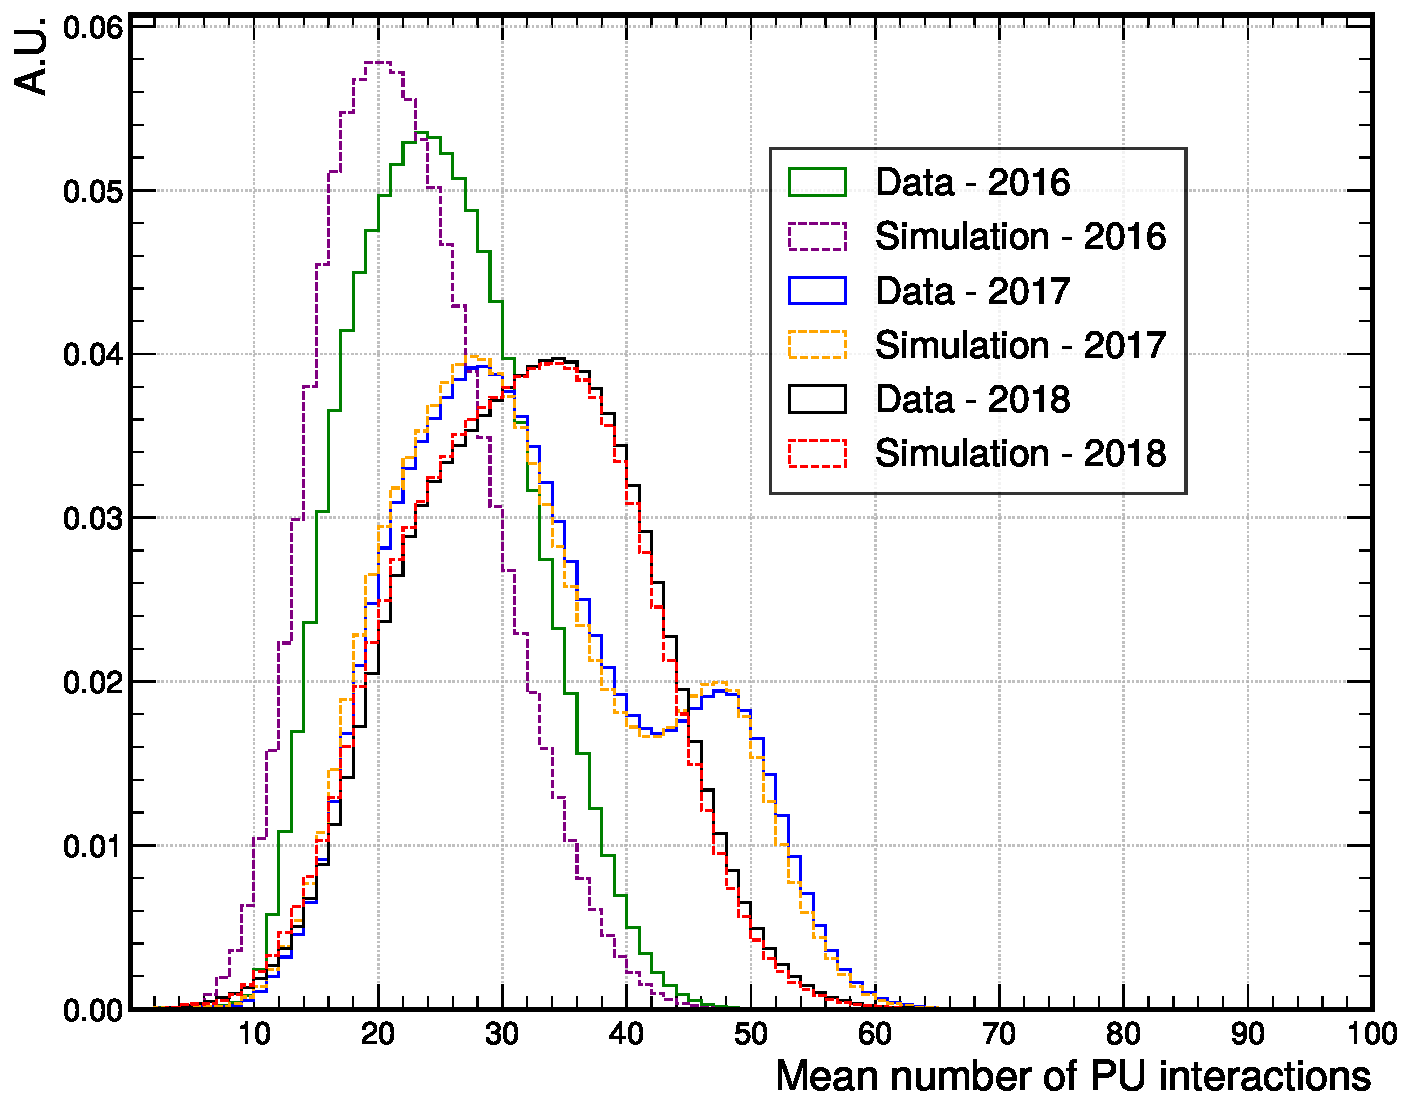
\includegraphics[width=0.8\textwidth]{Figures/Chapter6/PU_Profile.pdf}
\caption{Comparison of the distributions of the mean number of proton-proton interactions per bunch crossing between data and simulation in CMS Run 2.}
\label{Figure:Chapter6_PU_Profiles}
\end{figure}

\subsection{Electrons and Muons}
\label{Section:Chapter6_LightLepton_Corrections}

Although simulated light leptons are reconstructed using algorithms designed to replicate those used in data, residual differences remain and must be corrected. These corrections address different components of the reconstruction and selection process, including tracking, identification, isolation, and triggering.

Tracking corrections are derived centrally by the CMS collaboration and applied directly. However, all other electron and muon corrections are measured within this analysis using a dedicated implementation of the \textit{tag-and-probe} method~\cite{CMS_Muon_System_Performance,CMS_Muon_System_Performance_2}. This approach is necessary because the object selection criteria used in this analysis. Particularly, the impact parameter requirements on $d_{xy}$ and $d_z$ differ from those used in the official CMS efficiency measurements, as summarised in Table~\ref{Table:Chapter6_ObjectSelectionSummary}.

The tag-and-probe technique is applied to leptons from $\PZ \rightarrow \ell^+\ell^-$ decays, providing a clean and unbiased sample for assessing selection performance. Events are selected by requiring an opposite-charge, same-flavour lepton pair with invariant mass $m_{\ell\ell}$ between $65\GeV$ and $115\GeV$, enhancing the $\PZ$ boson purity. One lepton, the \textit{tag}, is required to pass tight identification, isolation, and single-lepton trigger criteria, ensuring it does not bias the measurement of the second lepton, the \textit{probe}. Both leptons are alternately assigned as tag and probe to increase statistical precision. Efficiencies are measured in bins of probe $p_{\mathrm{T}}$ and $\eta$ to account for detector and kinematic variations. The probe requirements for each selection stage are:

\begin{enumerate}[label=(\roman*)]
    \item Identification: Only requires identification
    \item Isolation: Requires identification, but not trigger.
    \item Trigger: Requires both identification and isolation.
\end{enumerate}

In each ($p_{\mathrm{T}}$, $\eta$) bin, events are split into ``pass'' and ``fail'' categories depending on whether the probe satisfies the selection under study. A simultaneous fit to the dilepton invariant mass distribution in both categories is used to extract the number of $\PZ \rightarrow \ell^+\ell^-$ signal events, accounting for residual background contamination. The signal is modelled with a sum of Voigtian functions, using the $\PZ$ boson’s natural width for the Breit-Wigner component. Backgrounds are modelled using:

\begin{itemize}
    \item A decaying exponential for the isolation and trigger fits.
    \item An error function transitioning to a decaying exponential for the identification fits, where background contamination is larger.
\end{itemize}

The efficiency is then extracted as:

\begin{equation_pad}
    \epsilon = \frac{N_{\text{pass}}}{N_{\text{pass}} + N_{\text{fail}}}
\end{equation_pad}

where $N_{\text{pass}}$ and $N_{\text{fail}}$ are the fitted $Z \rightarrow \ell^+\ell^-$ yields in each category. Figure~\ref{Figure:Chapter6-TagAndProbeFits_Nominal} shows an example fit for muons in a representative $\eta$ bin.

\begin{figure}[!htbp]
\centering
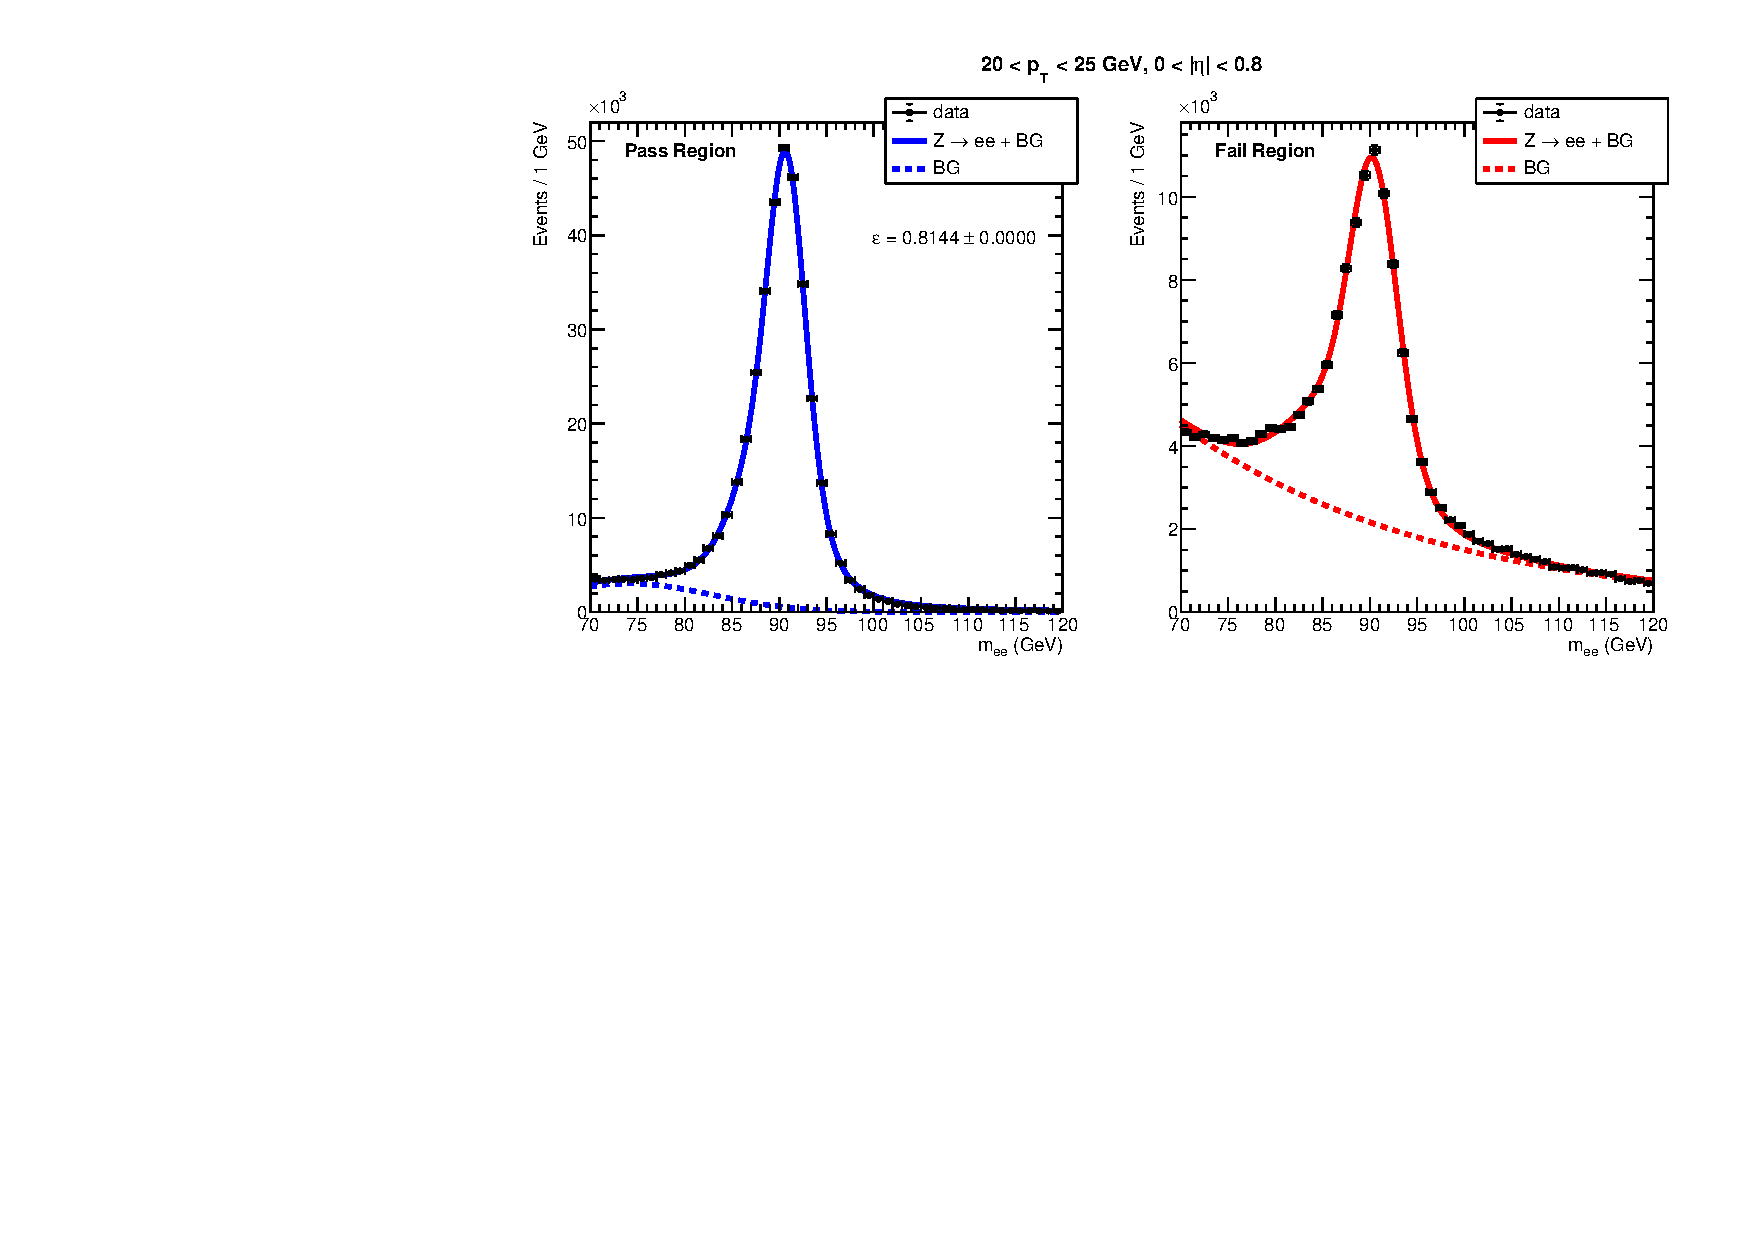
\includegraphics[width=\textwidth]{Figures/Chapter6/data_id_pt_20_to_25_eta_0.0_to_0.8_tpzee_nominal.pdf}
\caption{Example of the tag-and-probe fit used to extract electron identification efficiency in data. This plot corresponds to the $p_{\mathrm{T}}$ bin $20–25\GeV$ and the $|\eta|$ region 0.0–0.8.}
\label{Figure:Chapter6-TagAndProbeFits_Nominal}
\end{figure}

Efficiency SFs are then computed as the ratio of data and simulation efficiencies:

\begin{equation_pad}
    \text{SF}(p_\text{T},\eta) = \frac{\epsilon_\text{data}(p_\text{T},\eta)}{\epsilon_\text{MC}(p_\text{T},\eta)}
\end{equation_pad}

where these SFs are applied per object, and the total event-level correction is given by the product of the SFs for all leptons in the event.

Systematic uncertainties are estimated by varying aspects of the tag-and-probe procedure. These variations include modifying the tag lepton $p_{\text{T}}$ threshold (e.g., from $25\GeV$ to $35\GeV$), using alternative signal models, and changing the background parameterisation. Figure~\ref{Figure:Chapter6-TagAndProbeFits_Alternative} shows a representative comparison between the nominal fit configuration and a variant with a tighter tag lepton requirement. The resulting differences in efficiency are propagated as systematic uncertainties on the SFs.

\begin{figure}[!htbp]
    \centering
    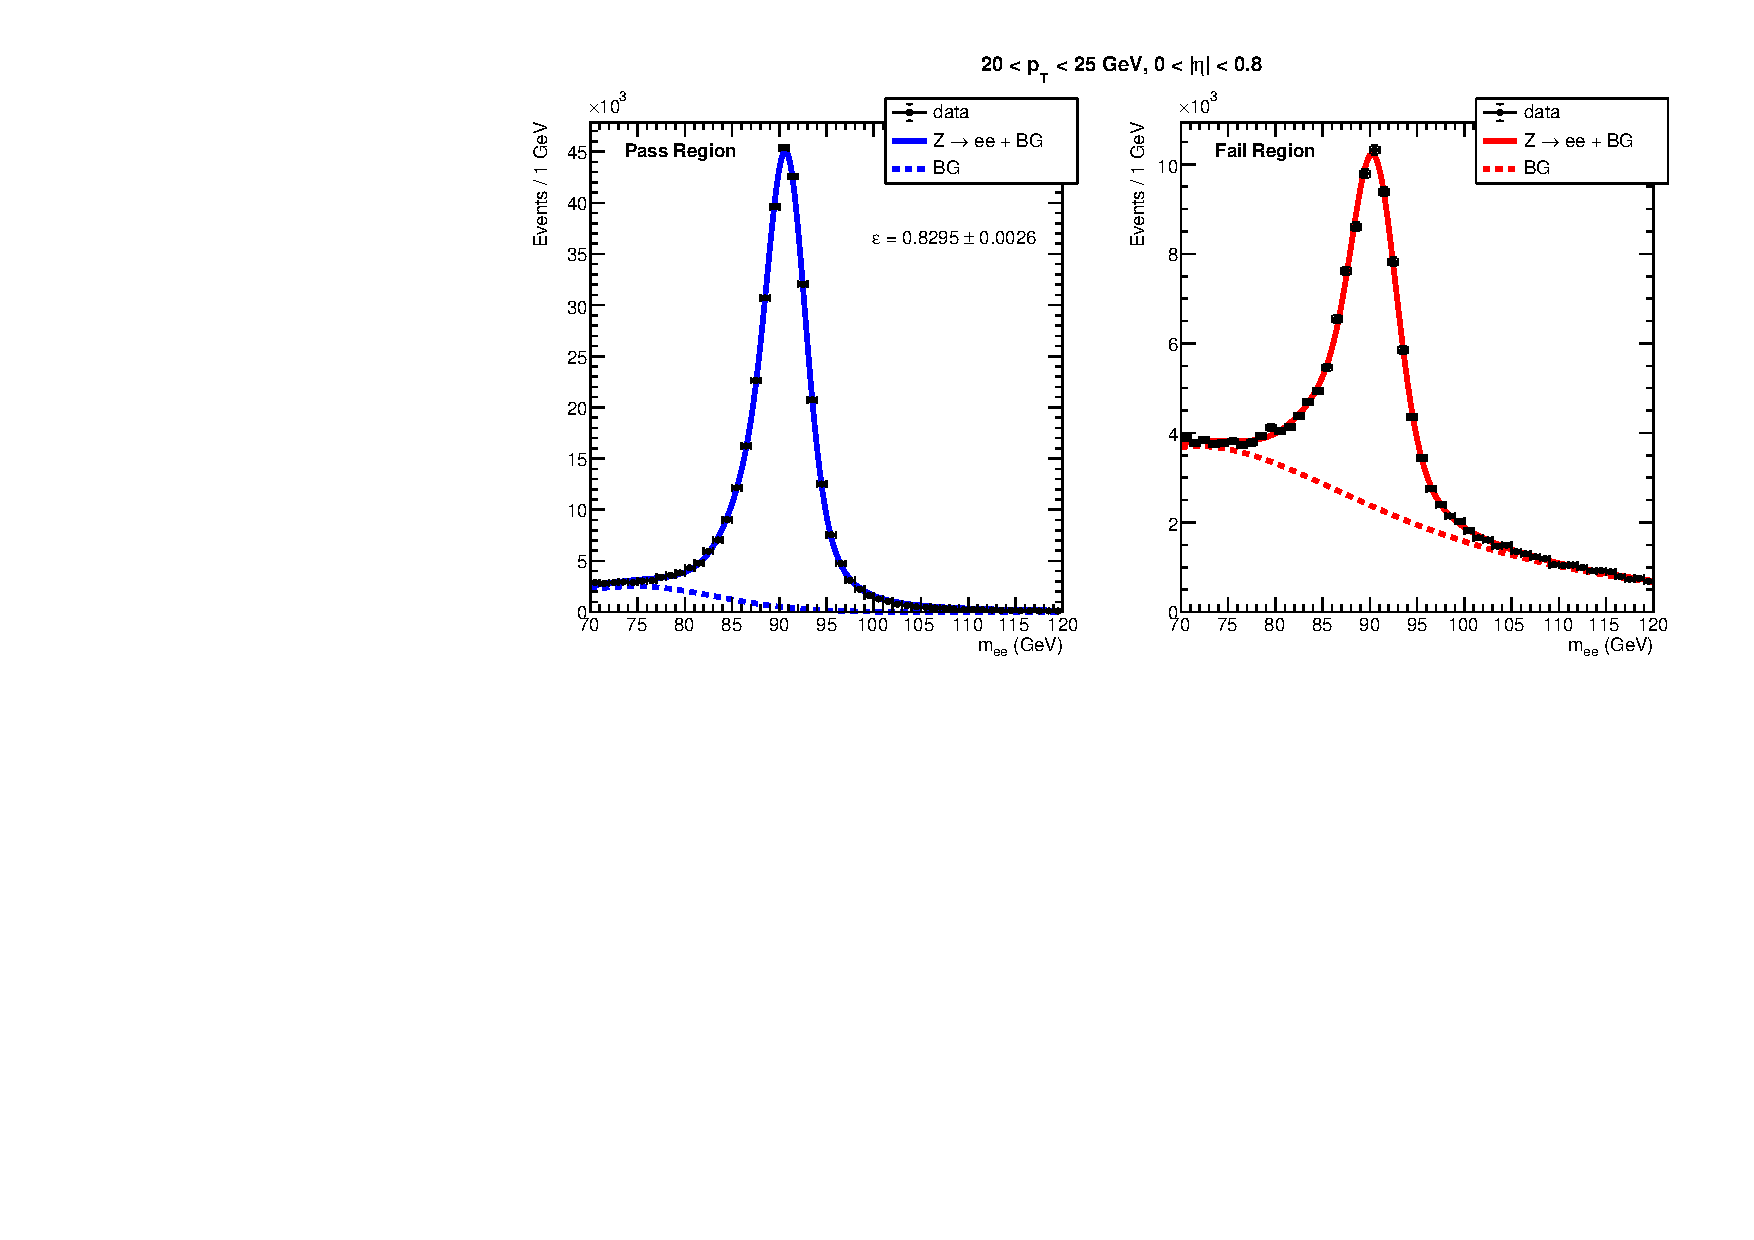
\includegraphics[width=\textwidth]{Figures/Chapter6/data_id_pt_20_to_25_eta_0.0_to_0.8_tpzee_tightTag.pdf}
    \caption[Impact of tag-and-probe configuration variations on efficiency extraction.]{Impact of tag-and-probe configuration variations on the measurement of electron identification efficiency in the $p_{\mathrm{T}}$ bin $20–25\GeV$ and $|\eta|$ region 0.0–0.8. Shown are invariant mass distributions and corresponding fits for a tighter tag lepton $p_\text{T}$ selection. These are compared to the nominal configuration shown in Fig.~\ref{Figure:Chapter6-TagAndProbeFits_Nominal}.}
    \label{Figure:Chapter6-TagAndProbeFits_Alternative}
\end{figure}

\subsection{Hadronic taus}

\subsubsection{Identification and energy Scale}
\label{Section:Chapter6_Tau_ID_ES}

Reliable modelling of $\PGt_h$ candidates is essential for accurate signal and background estimation in this analysis. As with electrons and muons (see Sections~\ref{Section:Electron_Identification} and~\ref{Section:Muon_Identification}), data-to-simulation corrections are applied in the form of SFs. These corrections are derived centrally by the CMS collaboration and are therefore only summarised here.

Identification scale factors are derived using a tag-and-probe method similar to that described for light leptons. In this case, $\PZ/\gamma^* \to \tau_\mu \tau_h$ events are used, where the muon serves as the tag and the $\PGt_h$ candidate as the probe. The visible mass of the muon–tau system, $m_{\text{vis}}$, is used as the primary observable. A binned maximum-likelihood fit to the $m_{\text{vis}}$ distribution, performed in the range $50 < m_{\text{vis}} < 150\GeV$, is used to extract the SF by comparing yields in data and simulation. To improve the robustness of the derivation, the fit is performed simultaneously with a control region enriched in $\PZ/\gamma^* \to \mu\mu$ events. The DY yield is treated with a common rate parameter across both regions, while the $\PGt_h$ ID SF is treated as the parameter of interest. Systematic uncertainties, including muon efficiency, luminosity, background normalisation, and MC statistics, are included as nuisance parameters. The resulting SFs are binned in HPS-assigned decay modes for $\pt^{\tauh} > 20\GeV$, accounting for variations across decay topologies and kinematic regions. 

In parallel, the \ac{TES} is extracted using external template fits. For each decay mode, a set of $m_{\text{vis}}$ templates is generated with varied TES values, and the best-fit value is determined via a likelihood scan. This TES is fixed when extracting the ID SFs. The resulting corrections typically fall within $\pm 2\%$, reflecting the high accuracy of CMS $\PGt_h$ energy reconstruction. Both of these corrections are applied to hadronic taus matched to genuine hadronic tau decays at the generator level.

In parallel, the \ac{TES} is extracted using external template fits. For each $\PGt_h$ decay mode, a set of $m_{\text{vis}}$ templates is generated with varied TES values, and the best-fit value is determined via a likelihood scan. This TES correction is then applied by shifting the four-momentum of $\PGt_h$ matched to genuine $\PGt_h$ decays at generator level. The extracted values are typically within $\pm 2\%$, reflecting the excellent agreement between data and simulation in CMS $\PGt_h$ energy reconstruction. The TES correction is fixed when extracting the ID SFs.

\subsubsection{Trigger}


Trigger efficiency corrections for $\PGt_h$ candidates are derived using $\PZ/\gamma^* \to \tau_\mu \tau_h$ events, exploiting the clean topology and well-identified muon leg. As with the identification and energy scale corrections, these are provided centrally by the CMS collaboration and are therefore only summarised here.

The efficiencies are measured using a tag-and-probe technique similar to that described for electrons and muons in Section~\ref{Section:Chapter6_LightLepton_Corrections}. The muon serves as the tag, while the hadronic tau is treated as the probe. To avoid introducing biases on the probe leg, dedicated \textit{monitoring triggers} are employed. These triggers impose stringent requirements on the muon while emulating the trigger logic applied to the tau leg, enabling an unbiased measurement of tau trigger performance.

Separate corrections are derived for lepton+tau and double-tau triggers. The resulting scale factors are applied to simulated events to correct for residual mismodelling in the trigger response.

\subsubsection{Lepton misidentification rates and energy scale}
\label{Section:Chapter6_Lepton_MisID_SF}

As introduced in Section~\ref{Section:Chapter6_Backgrounds}, prompt electrons and muons may be misidentified as $\PGt_h$ candidates by the DeepTau algorithm. Corrections for these misidentification rates are provided centrally by the CMS collaboration and are summarised here.

A tag-and-probe technique, similar in principle to that used for genuine leptons in Section~\ref{Section:Chapter6_LightLepton_Corrections}, is employed in $\PZ/\gamma^* \to ee$ and $\PZ/\gamma^* \to \mu\mu$ events. One lepton serves as the tag, while the other is required to be reconstructed as a $\tauh$ candidate. Events are then classified based on whether the probe passes the relevant DeepTau discriminator ($D_e$ or $D_\mu$). Misidentification rates are measured as a function of $\eta_{\tauh}$, and the data-to-simulation ratio defines the corresponding SFs. These are applied to simulated $\tauh$ candidates originating from misidentified electrons or muons, as identified through generator-level matching ($e \to \tauh$ or $\mu \to \tauh$).

Additionally, as in Section~\ref{Section:Chapter6_Tau_ID_ES}, dedicated energy scale corrections are applied to $\tauh$ candidates originating from misidentified electrons or muons, correcting for residual mismodelling of the reconstructed energy in simulation.

\subsection{B-tagging efficiency}

To correct for differences in $b$-tagging performance between data and simulation, jet-level SFs derived centrally by the CMS collaboration are applied. These SFs adjust the tagging efficiency for jets originating from $b$-quarks, $c$-quarks, and light-flavour partons. Rather than applying a global event weight, the tagging status of each jet is modified individually using a randomised procedure: jets are probabilistically promoted or demoted depending on whether the corresponding SF is greater or less than one. This approach ensures that the corrected jet collection reproduces data-like behaviour and can be used directly in event selection and categorisation without introducing additional per-event weights.

% This method is beneficial for analyses where the b-tag multiplicity defines the event category, since it allows for natural migration between categories and avoids complications associated with weighted event yields. However, it is not recommended in analyses that rely on variables which could become ill-defined when upgrading untagged jets—such as those involving secondary vertex information—since upgraded jets lack associated vertex reconstruction. Care must also be taken when SFs cross unity due to systematic variations, as this may affect the stability of such variables.


\section{Background modelling}
\label{Section:Chapter6_Background_Modelling}

As described in Section~\ref{Section:Chapter6_Backgrounds}, several processes can mimic the $Z^* \to \phi A \to 4\PGt$ signal signature, either through the presence of genuine $\PGt$ leptons, misidentified jets or light leptons reconstructed as $\PGt_h$ candidates, or a combination of both. This section outlines the strategies used to model these backgrounds and validate their contributions. For clarity, background processes are grouped into three main categories:


\begin{enumerate}[label=(\roman*)]

\item \textbf{Genuine-$\PGt$ backgrounds:} Events containing only genuine $\PGt$ leptons, primarily from $\PZ\PZ \to 4\PGt$, form an irreducible background and are estimated using simulation.

\item \textbf{Jet $\to \PGt_h$ misidentification:} Backgrounds with one or more jets misidentified as $\PGt_h$ candidates are modelled using a data-driven fake factor method.

\item \textbf{Lepton $\to \PGt_h$ misidentification:} Although subdominant, backgrounds from electrons or muons misidentified as $\PGt_h$ candidates can affect specific channels. These are estimated using simulation with dedicated corrections, as detailed in Section~\ref{Section:Chapter6_Lepton_MisID_SF}.

\end{enumerate}

\subsection{\texorpdfstring{Genuine-\boldmath{$\PGt$} backgrounds from $\PZ\PZ$}{Genuine tau backgrounds from ZZ}}
\label{Section:Chapter6_GenuineBackground}


These backgrounds arise predominantly from quark–antiquark annihilation, with a smaller contribution from gluon–gluon fusion. As discussed in Section~\ref{Section:Chapter6_Backgrounds}, these backgrounds, owing to their fully leptonic final state and close kinematic resemblance to the signal, are particularly challenging to suppress. As listed in Table~\ref{Table:Chapter6_SimulatedBackgrounds}, the quark-initiated process is simulated using \POWHEG at NLO in QCD, while the gluon-initiated component is generated at LO with \PYTHIA. To account for missing higher-order effects, both samples are corrected using multiplicative $\mathcal{K}$-factors~\cite{Kfactors_ZZ} applied as a function of the four-lepton invariant mass, $m_{4\ell}$:

\begin{itemize}
\item Quark-initiated $\PZ\PZ$:  A mass-dependent NLO-to-NNLO QCD $\mathcal{K}$-factor derived from \POWHEG~2.0\cite{Powheg_1,Powheg_2} is applied, with a typical value of around 1.2 across the relevant phase space.
\item Gluon-initiated $\PZ\PZ$: A larger $\mathcal{K}$-factor, typically 2.0, is applied to match NNLO predictions from \textsc{HNNLO v2}\cite{PhysRevLett.98.222002}.
\end{itemize}

Simulation is validated in a control region enriched in $\PZ\PZ \to \mu^+\mu^-\mu^+\mu^-$, which provides a clean signature with minimal background contamination. The standard object selection criteria (see Table~\ref{Table:Chapter6_ObjectSelectionSummary}) are applied, with one targeted modification: the muon isolation requirement is relaxed to $I^\mu_\text{PF} < 0.35$ to enhance statistical precision. The total charge of the four-muon system is also required to be zero. Additionally, the trigger configuration used in this region is detailed in Table~\ref{Table:Chapter6_TriggersPerChannel}. Figure~\ref{Figure:Chapter6_ZZ_KfactorImpact} illustrates how applying $\mathcal{K}$-factors improves the agreement between simulation and data in the invariant mass distribution of the four-muon system.

\begin{figure}[!htbp]
        \centering
        % First row
        \begin{subfigure}[b]{0.49\textwidth}
            \centering
            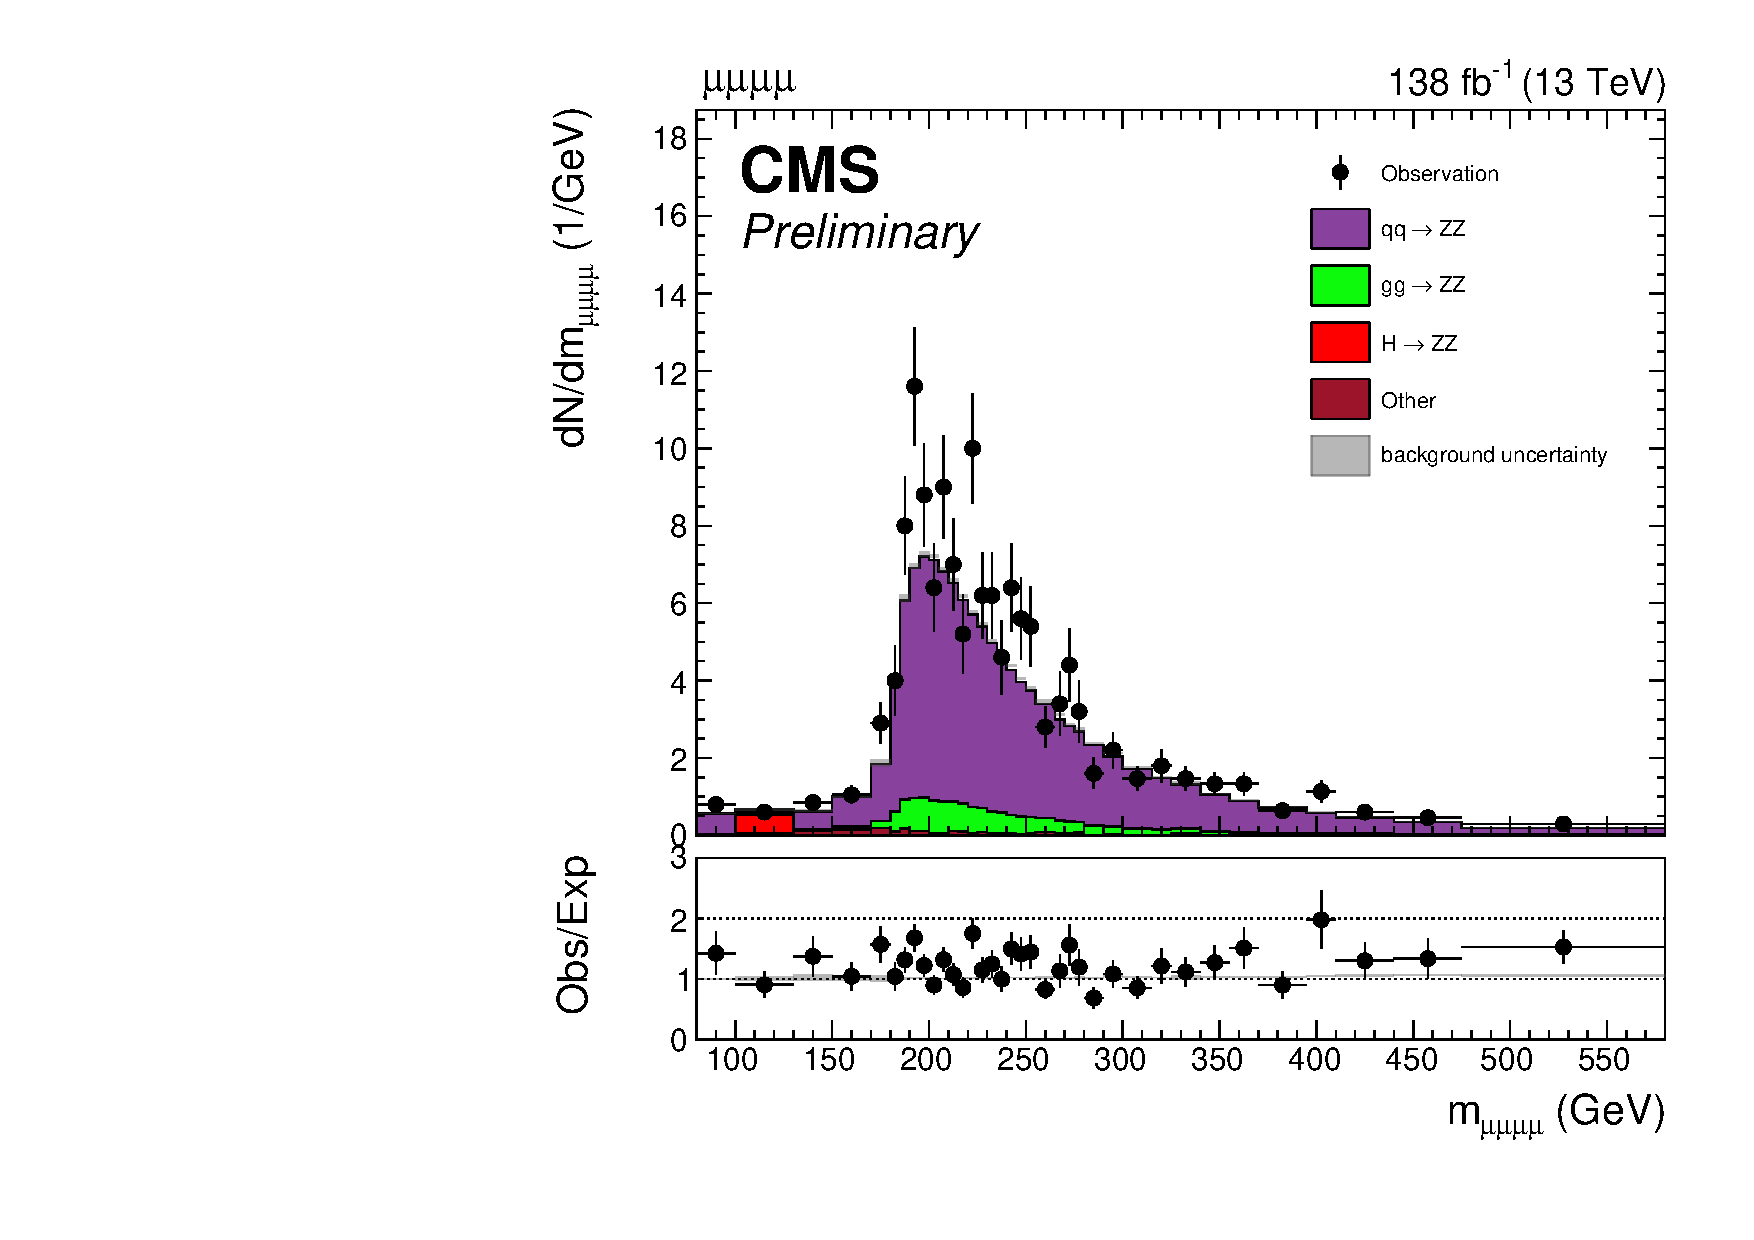
\includegraphics[width=\textwidth]{Figures/Chapter6/mmmm_wo_kfactors.pdf}
            \caption{}
        \end{subfigure}
        \vspace{0.5cm}
        \begin{subfigure}[b]{0.49\textwidth}
            \centering
            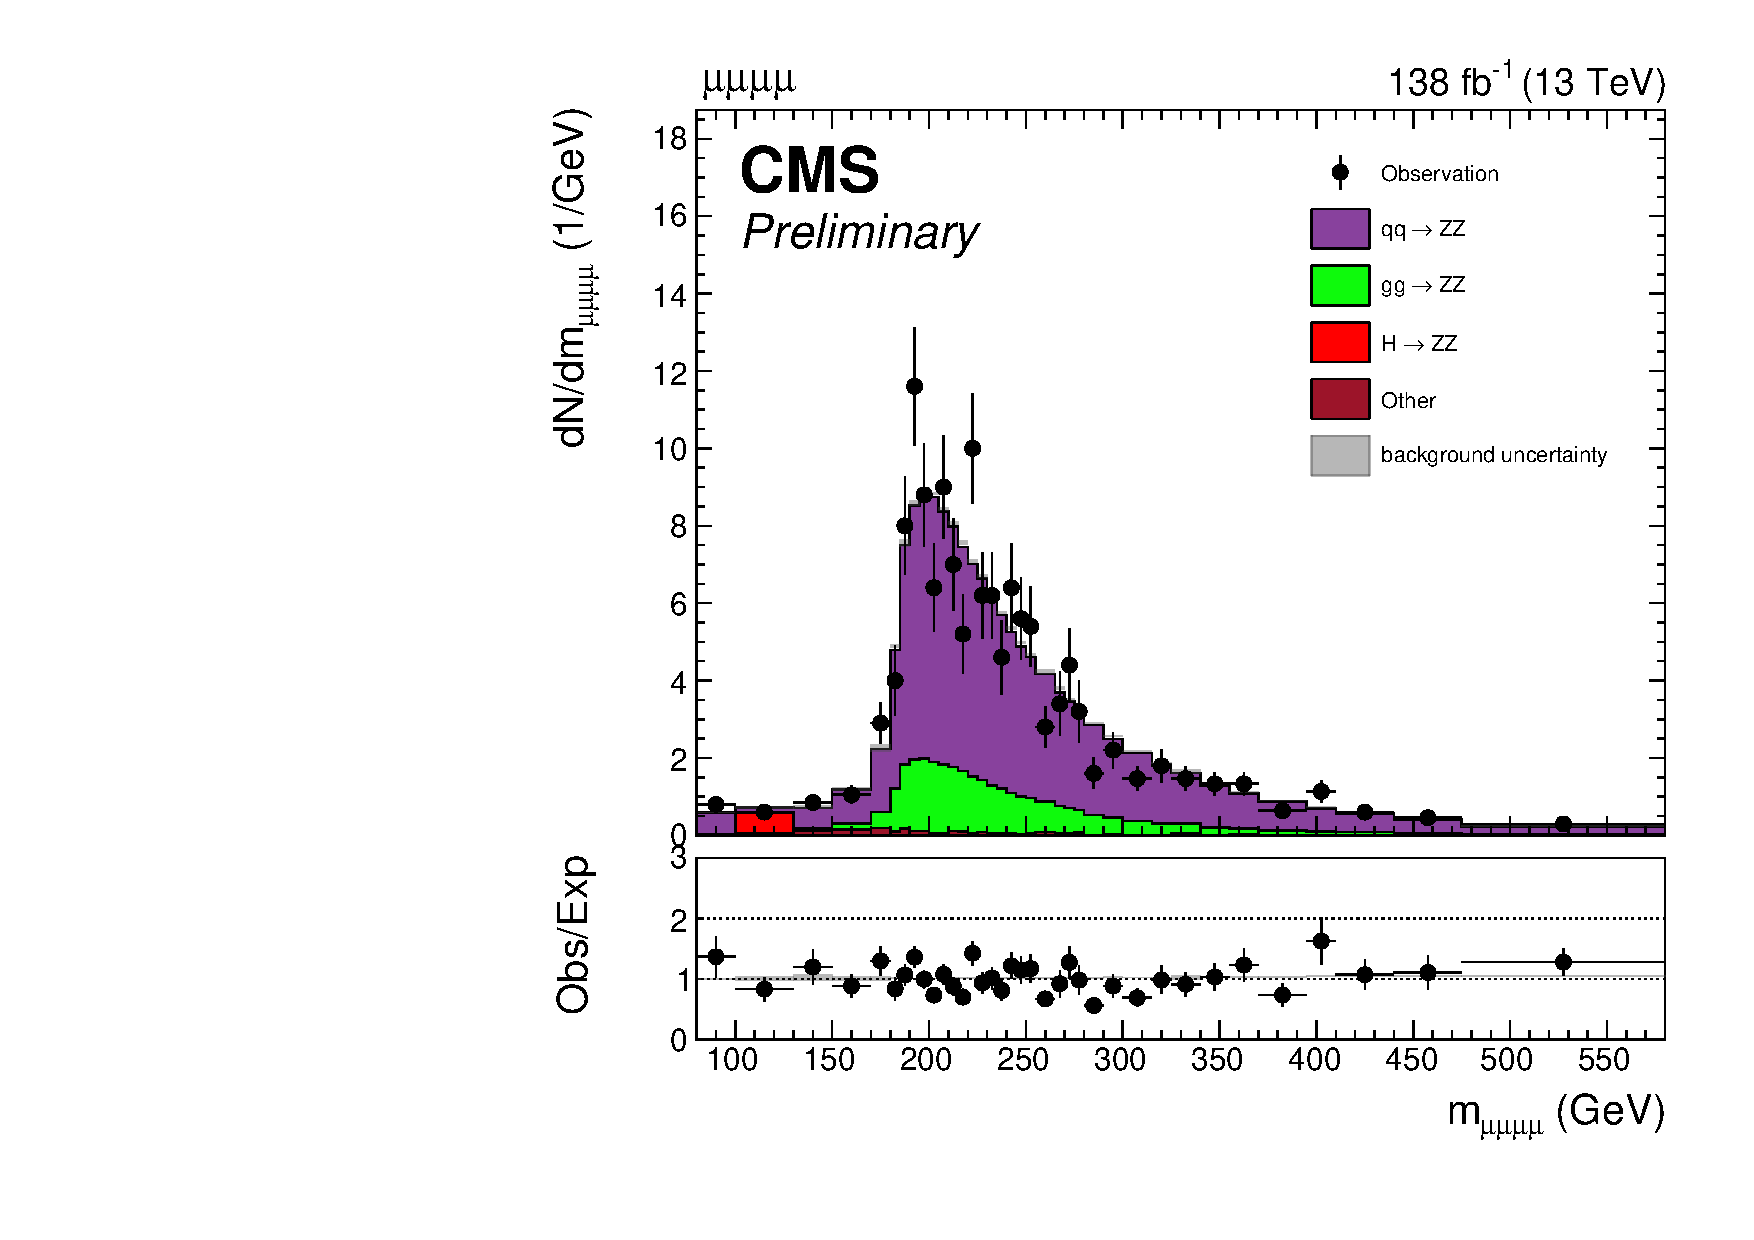
\includegraphics[width=\textwidth]{Figures/Chapter6/mmmm_with_kfactors.pdf}
            \caption{}
        \end{subfigure}
    \caption[Impact of $\mathcal{K}$-factors on the $\PZ\PZ$ background prediction in the four-muon control region.]{Impact of $\mathcal{K}$-factors on the $\PZ\PZ$ background prediction in the four-muon control region. Shown are the invariant mass distributions of the $\mu^+\mu^-\mu^+\mu^-$ system before (\textbf{a}) and after (\textbf{b}) applying $\mathcal{K}$-factors.}
    \label{Figure:Chapter6_ZZ_KfactorImpact}
\end{figure}

While $\PZ\PZ$ constitutes an irreducible background, it can still be reduced through targeted kinematic selections. For example, in the $\PGt_e\PGt_h\PGt_h\PGt_h$ channel, signal events tend to exhibit harder $p_{\mathrm{T}}$ spectra for subleading leptons. The object selection thresholds conveniently exploit this difference. As illustrated in Figure~\ref{Figure:Chapter6_ThirdLepPt}, applying a $p_{\mathrm{T}}$ cut at $20\GeV$ significantly reduces this background while preserving the majority of the signal.

\begin{figure}[!htbp]
    \centering
    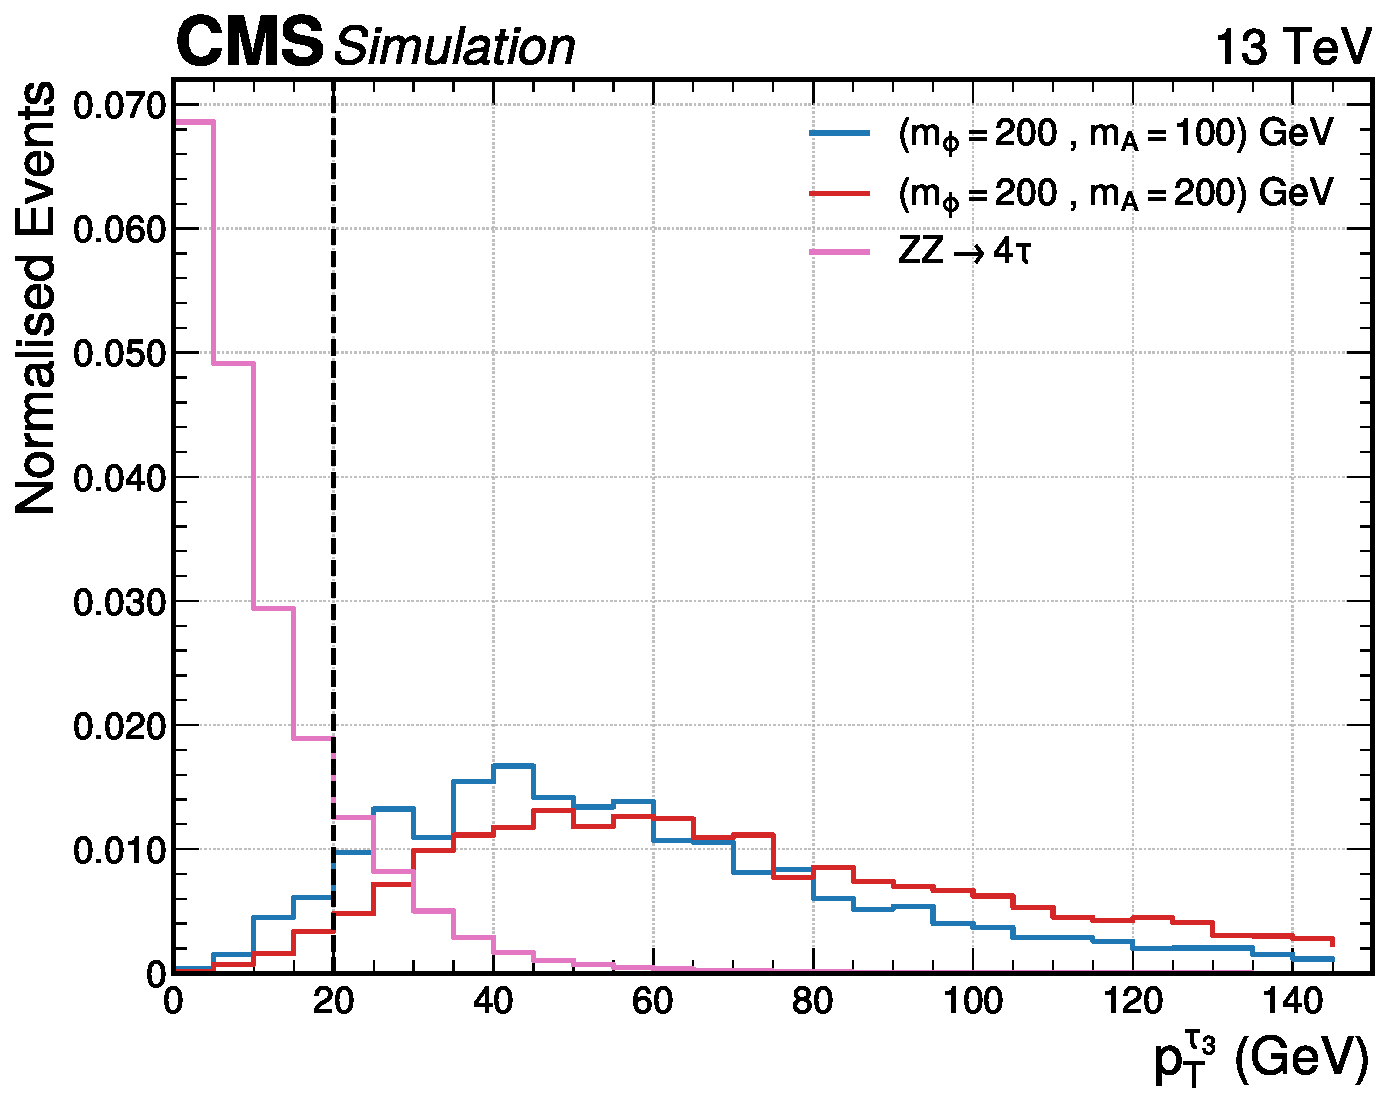
\includegraphics[width=0.6\textwidth]{Figures/Chapter6/ZZ_OfflineCutImpact.pdf}
    \caption[$p_{\mathrm{T}}$ spectrum of the third lepton in the $\PGt_e\PGt_h\PGt_h\PGt_h$ channel.]{Distribution of the transverse momentum of the third lepton in the $\PGt_e\PGt_h\PGt_h\PGt_h$ channel, comparing the expected $\PZ\PZ$ background to the signal prediction. The solid line at $20\GeV$ region indicates the $p_{\mathrm{T}}$ selection threshold applied.}
    \label{Figure:Chapter6_ThirdLepPt}
\end{figure}

\subsection{\texorpdfstring{Background from Jets Misidentified as $\PGt_h$ (Jet $\to \PGt_h$)}{Background from Jets Misidentified as hadronic taus}}

\label{Section:Chapter6_JetToTauBackground}

This section discusses how the background from jets misidentified as $\PGt_h$ candidates is modelled. These backgrounds arise from misidentified jets from processes such as the ones outlined in Section~\ref{Section:Chapter6_Backgrounds}. Such misidentifications are particularly problematic to model in simulation, as the jet-to-$\PGt_h$ misidentification rate is poorly described in MC simulations. Moreover, the small probability of such a jet misidentification makes it necessary to generate high-statistics MC samples, which come with a significant computational expense. These limitations and the difficulty in capturing the full range of misidentification scenarios in simulation motivate the use of a data-driven approach, such as the Fake Factor ($F_F$) method.

\subsubsection{Classical Fake Factor Method}
\label{Section:Chapter6_FakeFactors_Classical}

The classical $F_F$ approach begins by defining a dedicated \ac{DR}, enriched in jet$\to\PGt_h$ events. Any non-jet$\to\PGt_h$ contributions are estimated using simulation and subtracted to isolate the misidentified component, ensuring a pure region. In this region, the $F_F$ is computed as the ratio of events passing a \texttt{Nominal} tau ID requirement to those failing it but satisfying a looser \texttt{Alternative} ID:

\begin{equation}
F_F = \frac{\mathcal{N}(\texttt{Nominal})}{\mathcal{N}(\texttt{Alternative and not Nominal})}
\end{equation}

The choice of the alternative identification requirement introduces a trade-off. Looser identification thresholds reduce the statistical uncertainty by increasing the number of events in the denominator. However, this comes at the cost of increased systematic uncertainty, as the looser $\PGt_h$ candidates are less representative of those in the SR. 

Regarding its determination, the $F_F$ is computed differentially in key variables such as $p_\text{T}$, jet multiplicity ($\mathcal{N}_{\text{jets}}$), and other observables that parametrise the misidentification rate. Since the $F_F$ can also depend on the definition of the DR, additional corrections are often derived in sideband regions to mitigate residual dependencies and improve the robustness of the estimate. The $F_F$ is then applied to the \ac{AR}, which is constructed to resemble the SR. Specifically, the AR requires the $\PGt_h$ candidates to pass the \texttt{Alternative} ID and fail the \texttt{Nominal} one. This enables a fully data-driven estimate of the jet-induced background in the SR.

Despite its simplicity and robustness, the classical method faces several limitations:

\begin{itemize}
\item \textit{Curse of dimensionality}: Including more variables in the parameterisation rapidly inflates the number of bins, leading to sparse statistics and unstable estimates.

\item \textit{Correlations}: Variables not explicitly included in the fit may be poorly modelled. Corrections in one observable can worsen agreement in another, highlighting the limitations of low-dimensional approaches that fail to capture correlations.

\item \textit{Scalability in multi-$\PGt_h$ final states}: In channels like $\PGt_h \PGt_h \PGt_h \PGt_h$, the method becomes increasingly cumbersome. A separate $F_F$ must be computed for each $\PGt_h$ candidate, applied iteratively. This procedure becomes statistically challenging in low-yield regimes and complicates the estimate.
\end{itemize}

These challenges were noted in previous CMS analyses of ditau final states~\cite{CMS:2022goy,Mb:2022rxu}, where a $F_F$ was typically derived for, and applied to, the leading $\PGt_h$ candidate. This approach could not account for cases in which the leading object was genuine and the subleading object was a misidentified jet. Such events had to be modelled using simulation. While this simplification was acceptable in those studies due to the subdominant contribution of such configurations, it becomes insufficient in this analysis, where final states often involve multiple misidentified $\PGt_h$ candidates. A more general, high-dimensional approach is therefore required to reliably account for all sources of jet$\to\PGt_h$ misidentification.


\subsubsection{Machine Learning-based reweighting}
\label{Section:Chapter6_FakeFactors_BDT}

To overcome the limitations of binning-based methods, misidentification rates can be estimated using \ac{ML}-based density ratio estimation. The objective is to model the misidentification rate as a function of multiple observables. Mathematically, this corresponds to estimating the ratio of probability densities $f_{\text{pass}}(x)/f_{\text{fail}}(x)$.

\begin{equation_pad}
\frac{f_{\text{pass}}(x)}{f_{\text{fail}}(x)} \sim \frac{p_{\text{pass}}(x)}{p_{\text{fail}}(x)}.
\end{equation_pad}

This ratio can be approximated using classifiers such as \acp{BDT}, where the class probabilities serve as a proxy for the density ratio. However, standard classifiers often underperform in regions where the density ratio is large (\ie where one class dominates). In such regions, the classification task becomes trivial, and the model focuses its learning on harder, more ambiguous regions where classes are balanced. These easy-to-classify regions receive little weight in the loss function (typically cross-entropy), leading to poor modelling precisely where accurate reweighting is most critical.

To mitigate this, a custom objective function is introduced that directly targets discrepancies between the pass and fail distributions. In tree-based models, this objective is optimised over sets of events grouped into leaves\footnote{Leaves are the terminal nodes of a decision tree; each leaf contains events satisfying the same set of decision rules.}. This objective function is the symmetrised $\chi^2$ metric, which prioritises leaves with the largest differences between the two samples:

\begin{equation_pad}
    \chi^2 = \sum_{\text{leaf}} \frac{(w_{\text{leaf}, \text{fail}} - w_{\text{leaf}, \text{pass}})^2}{w_{\text{leaf}, \text{fail}} + w_{\text{leaf}, \text{pass}}}
\end{equation_pad}

where $w_{\text{leaf}, \text{fail}}$ and $w_{\text{leaf}, \text{pass}}$ are the total event weights in each leaf from the fail and pass samples, respectively. Maximising this objective during training steers the model toward the regions most relevant for improving reweighting accuracy.

Training proceeds in a boosting-like fashion, where a series of shallow decision trees is built sequentially. Each tree addresses discrepancies not corrected by previous ones. At each iteration, the following steps are performed:

\begin{enumerate}[label=(\roman*)]
    \item A shallow decision tree that maximises the symmetrised $\chi^2$ is built.
    \item For each leaf, the log-ratio of total weights ($r_\text{leaf}$) is computed:
    \item The weights of fail-sample events in each leaf are updated: $w = w \times e^{r{_\text{leaf}}}$.
\end{enumerate}

This procedure is iterated multiple times, allowing the model to refine the reweighting progressively by targeting residual discrepancies in each step.

\subsubsection{Fitting and Parametrisation}
\label{Section6:Fitting_Parametrisation}
Having introduced the ML-based reweighting approach, this section outlines its implementation in the context of this analysis. This includes the definition of fitting regions and the choice of input variables for training. As described in Section~\ref{Section:Chapter6_FakeFactors_Classical}, the classical $F_F$ method relies on defining a set of control regions. These regions can be organised into an ABCD-style framework, as illustrated in Figure~\ref{Figure:Chapter6_ABCD}, with sidebands constructed from variables such as hadronic tau identification and total charge.

\begin{figure}[!htbp]
\centering
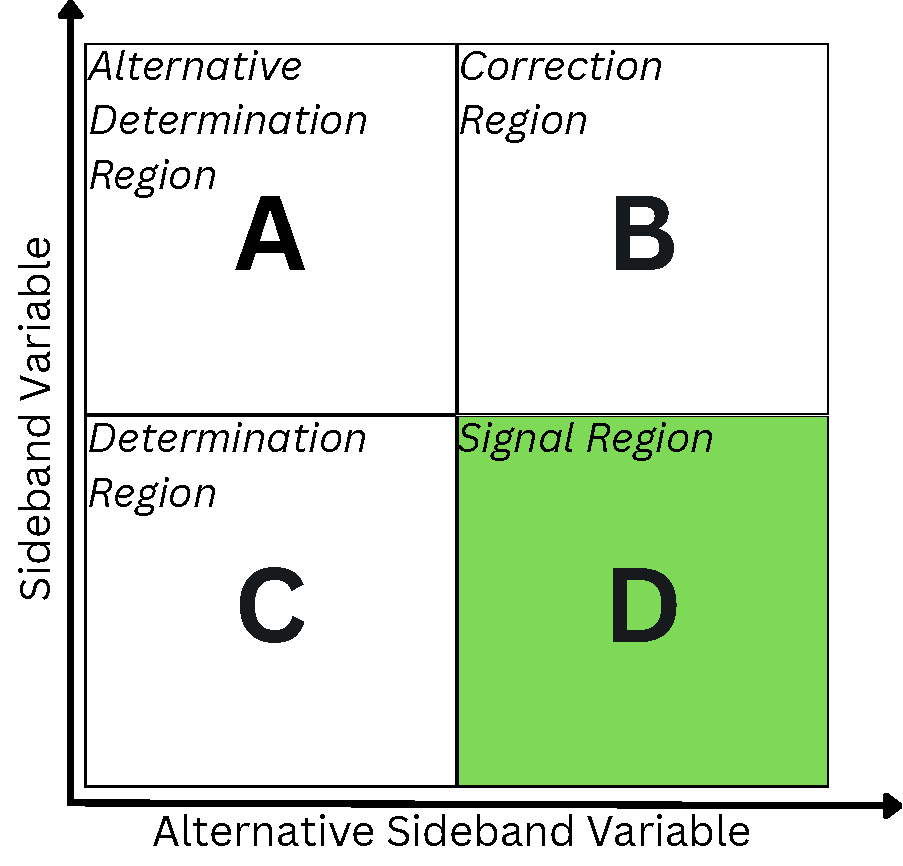
\includegraphics[width=0.6\textwidth]{Figures/Chapter6/ABCD.pdf}
\caption[ABCD-style region definition for fake factor estimation.]{Schematic illustration of an ABCD-style region definition used in the fake factor method.}
\label{Figure:Chapter6_ABCD}
\end{figure}

The channel-specific sideband selections used to define these regions are summarised below:

\begin{enumerate}[label=(\roman*)]
    \item For the channels: $\PGt_e\PGt_h\PGt_h\PGt_h$, $\PGt_e\PGt_e\PGt_h\PGt_h$, $\PGt_e\PGt_\mu\PGt_h\PGt_h$, $\PGt_\mu\PGt_h\PGt_h\PGt_h$, $\PGt_\mu\PGt_\mu\PGt_h\PGt_h$, and $\PGt_h\PGt_h\PGt_h\PGt_h$:
    \begin{itemize}
    \item \textbf{Region A (SR-like)}: \\
    All alternative\footnote{``Alternative'' refers to all other hadronic taus in the event for which the $F_F$ is not currently being derived.} hadronic taus pass the \texttt{Nominal} tau ID; $\sum q_{\PGt_h} = 0$.

    \item \textbf{Region B (Inverted Identification)}: \\
    At least one alternative hadronic tau fails the \texttt{Nominal} tau identification but passes the \texttt{Alternative} selection; $\sum q = 0$.

    \item \textbf{Region C (Inverted Charge)}: \\
    All alternative $\PGt_h$ hadronic taus pass the \texttt{Nominal} tau ID; charge sum requirement is $\sum q \neq 0$.

    \item \textbf{Region D (Inverted ID and Charge)}: \\
    At least one alternative hadronic tau fails the \texttt{Nominal} tau ID but passes the \texttt{Alternative} selection; $\sum q \neq 0$.
    \end{itemize}

    \item For the $\PGt_h\PGt_h\PGt_h$ channel, the same ID criteria apply, but the charge requirement is modified:
    \begin{itemize}
        \item \textbf{Region A/B}: $|\sum q \,| = 1$
        \item \textbf{Region C/D}: $|\sum q\,| \neq 1$
    \end{itemize}
\end{enumerate}

While this framework is conceptually straightforward for deriving the $F_F$ for a single $\PGt_h$ candidate, it becomes increasingly complex in multi-$\PGt_h$ events as discussed in Section~\ref{Section:Chapter6_FakeFactors_Classical}. Each candidate must be treated separately, with its own ABCD categorisation defined in terms of the others. This results in multiple overlapping sets of control regions that must be constructed within the same event.

The ML approach circumvents these issues entirely by eliminating the need for explicit ABCD definitions. Each $\PGt_h$ candidate is treated as an independent training instance, contributing a single row to the training dataset. Both candidate-level and event-level features, including those used in traditional ABCD axes, are passed directly to the model. This enables the algorithm to learn a flexible, high-dimensional reweighting function across the entire parameter space without fragmenting the data. The features used for training are grouped as follows:

\begin{enumerate}[label=(\roman*)]

    \item \textbf{Properties of the target $\PGt_h$ candidate:} The target $\PGt_h$ candidate is characterised by several features: its HPS decay mode, $p_\text{T}^{\PGt_h}$,  $\eta$, electric charge, and whether it satisfies the relevant leg of the double-$\tau$ trigger. Additionally, the ratio of the $p_\text{T}$ of the seeding jet to that of the $\PGt_h$ candidate ($p_\text{T}^\text{jet} / p_\text{T}^{\PGt_h}$) is included.

    \item \textbf{Sideband-specific variables:}
    \begin{itemize}
        \item Total charge of all $\PGt_h$ candidates
        \item A boolean indicating whether the DeepTau discriminator of the alternative hadronic taus (sorted by $p_\text{T}$) passes the \texttt{Nominal} tau identification requirement
    \end{itemize}

    \item \textbf{Global event variables:}
    \begin{itemize}
        \item Data-taking period identifier
        \item $p_\text{T}$ rank of the target hadronic tau in the event
    \end{itemize}

\end{enumerate}

\subsubsection{\texorpdfstring{Non-jet$\to \PGt_h$ background removal}{Non-jet to hadronic tau background removal}}

As noted in Section~\ref{Section:Chapter6_FakeFactors_Classical}, backgrounds from non-jet$\to\PGt_h$ candidates are traditionally removed by subtracting simulated events from data at the histogram level. However, this approach is not compatible with the ML-based method, which operates on full unbinned datasets and does not support negative event weights. One possible workaround is template matching, where a simulated non-jet$\to\PGt_h$ candidate for every matching data event is removed to emulate histogram subtraction at the event level. Yet, this method is computationally infeasible given the high dimensionality of the input space and the size of the datasets.

Instead, a binary BDT is trained to distinguish jet$\to\PGt_h$ from non-jet$\to\PGt_h$ candidates, using the same input variables as the main reweighting model. This reduces the classification problem to a single discriminant: the BDT score, which quantifies how ``non-jet$\to\PGt_h$-like'' each candidate is. The trained BDT is applied to both simulation and data. A histogram of BDT scores is constructed from simulated non-jet$\to\PGt_h$ candidates and normalised to the expected cross section, yielding a bin-by-bin prediction of the expected contamination in data. The same BDT is then applied to data, and for each bin of the BDT score distribution, data events falling within that range are randomly sampled and removed. This is repeated until the number of removed events matches the predicted contamination in that bin.

The result is a purified dataset of jet$\to\PGt_h$-like candidates, closely mimicking the effect of histogram-level subtraction but in a form that remains compatible with the ML-based reweighting method. Figure~\ref{Figure:Chapter6_BDTPurificationExample} compares this strategy with the traditional subtraction method, demonstrating their agreement.

\begin{figure}[!htbp]
        \centering
        % First row
        \begin{subfigure}[b]{0.49\textwidth}
            \centering
            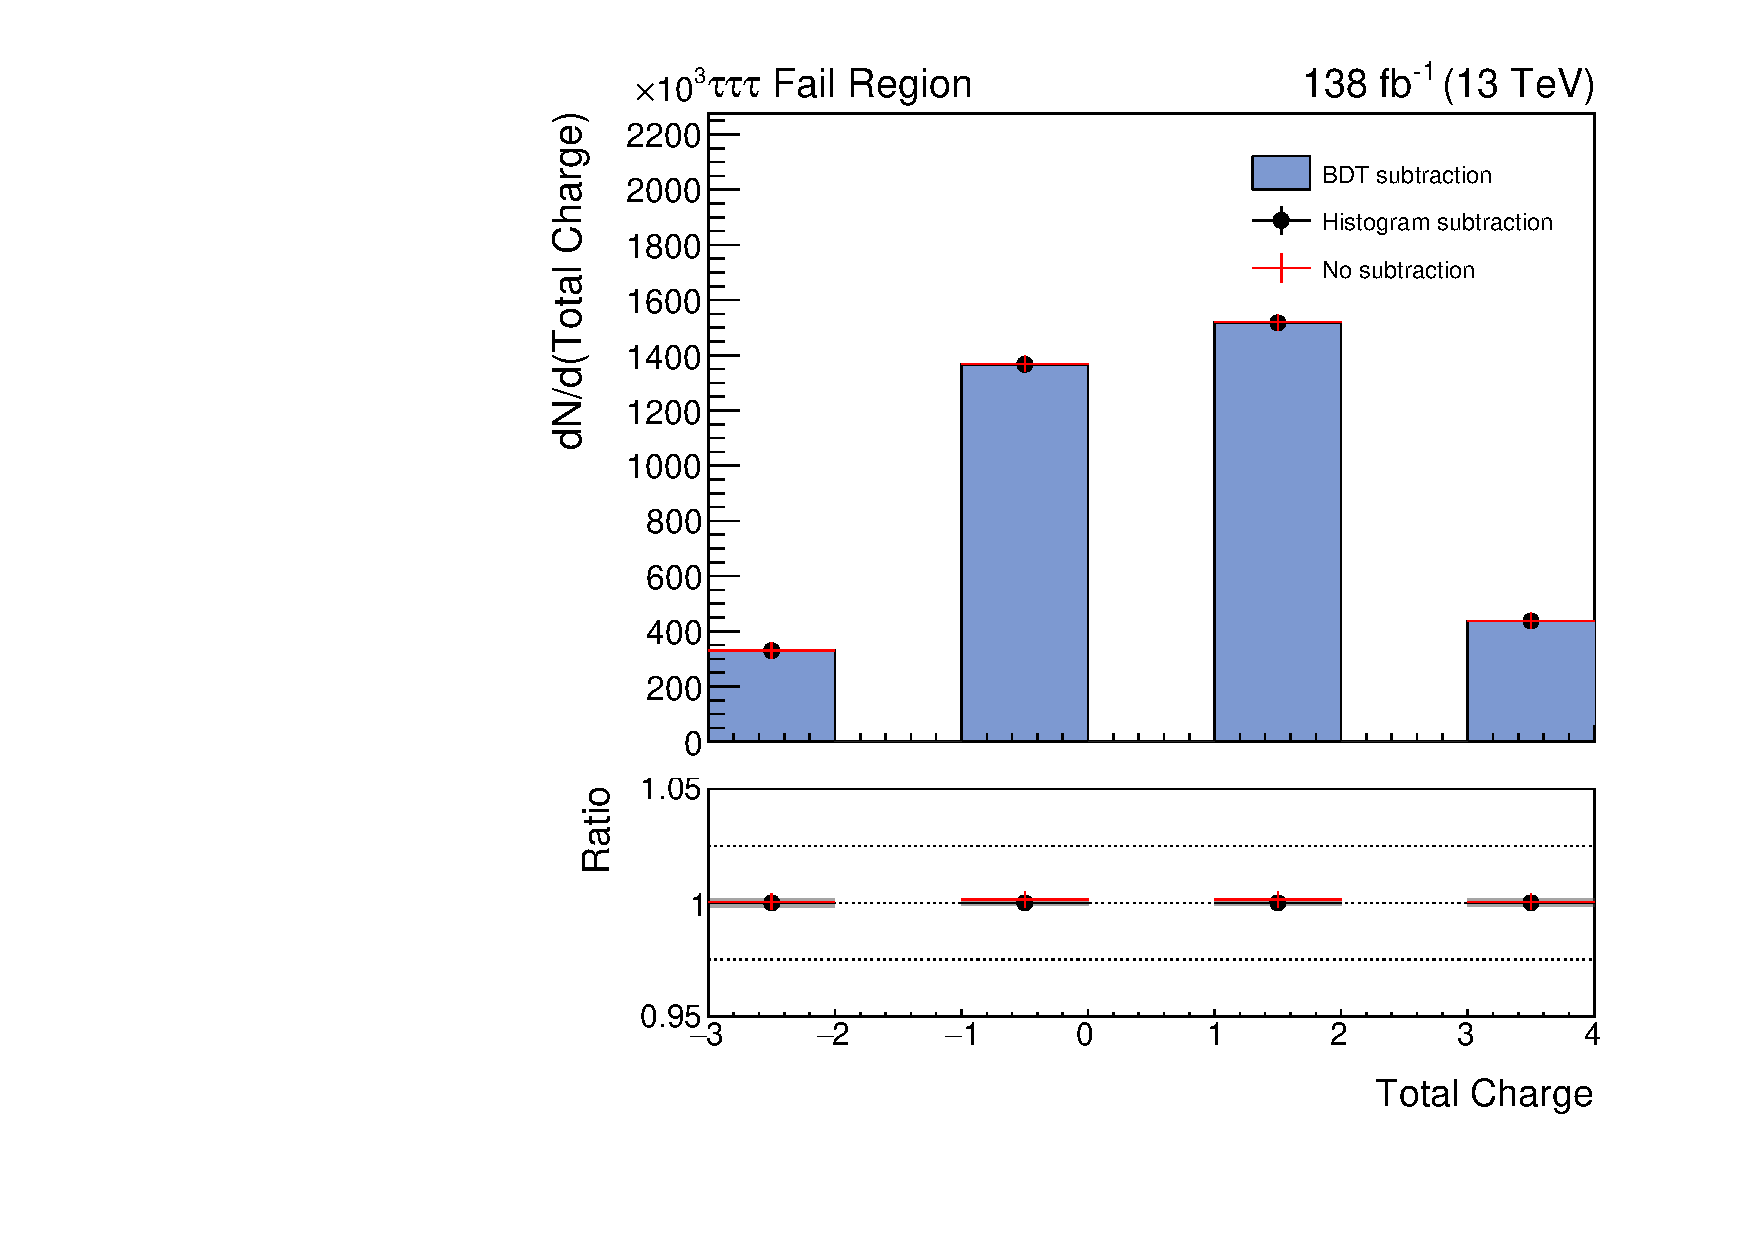
\includegraphics[width=\textwidth]{Figures/Chapter6/subtraction_plot_q_sum_ttt_fail.pdf}
            \caption{}
        \end{subfigure}
        \vspace{0.5cm}
        \begin{subfigure}[b]{0.49\textwidth}
            \centering
            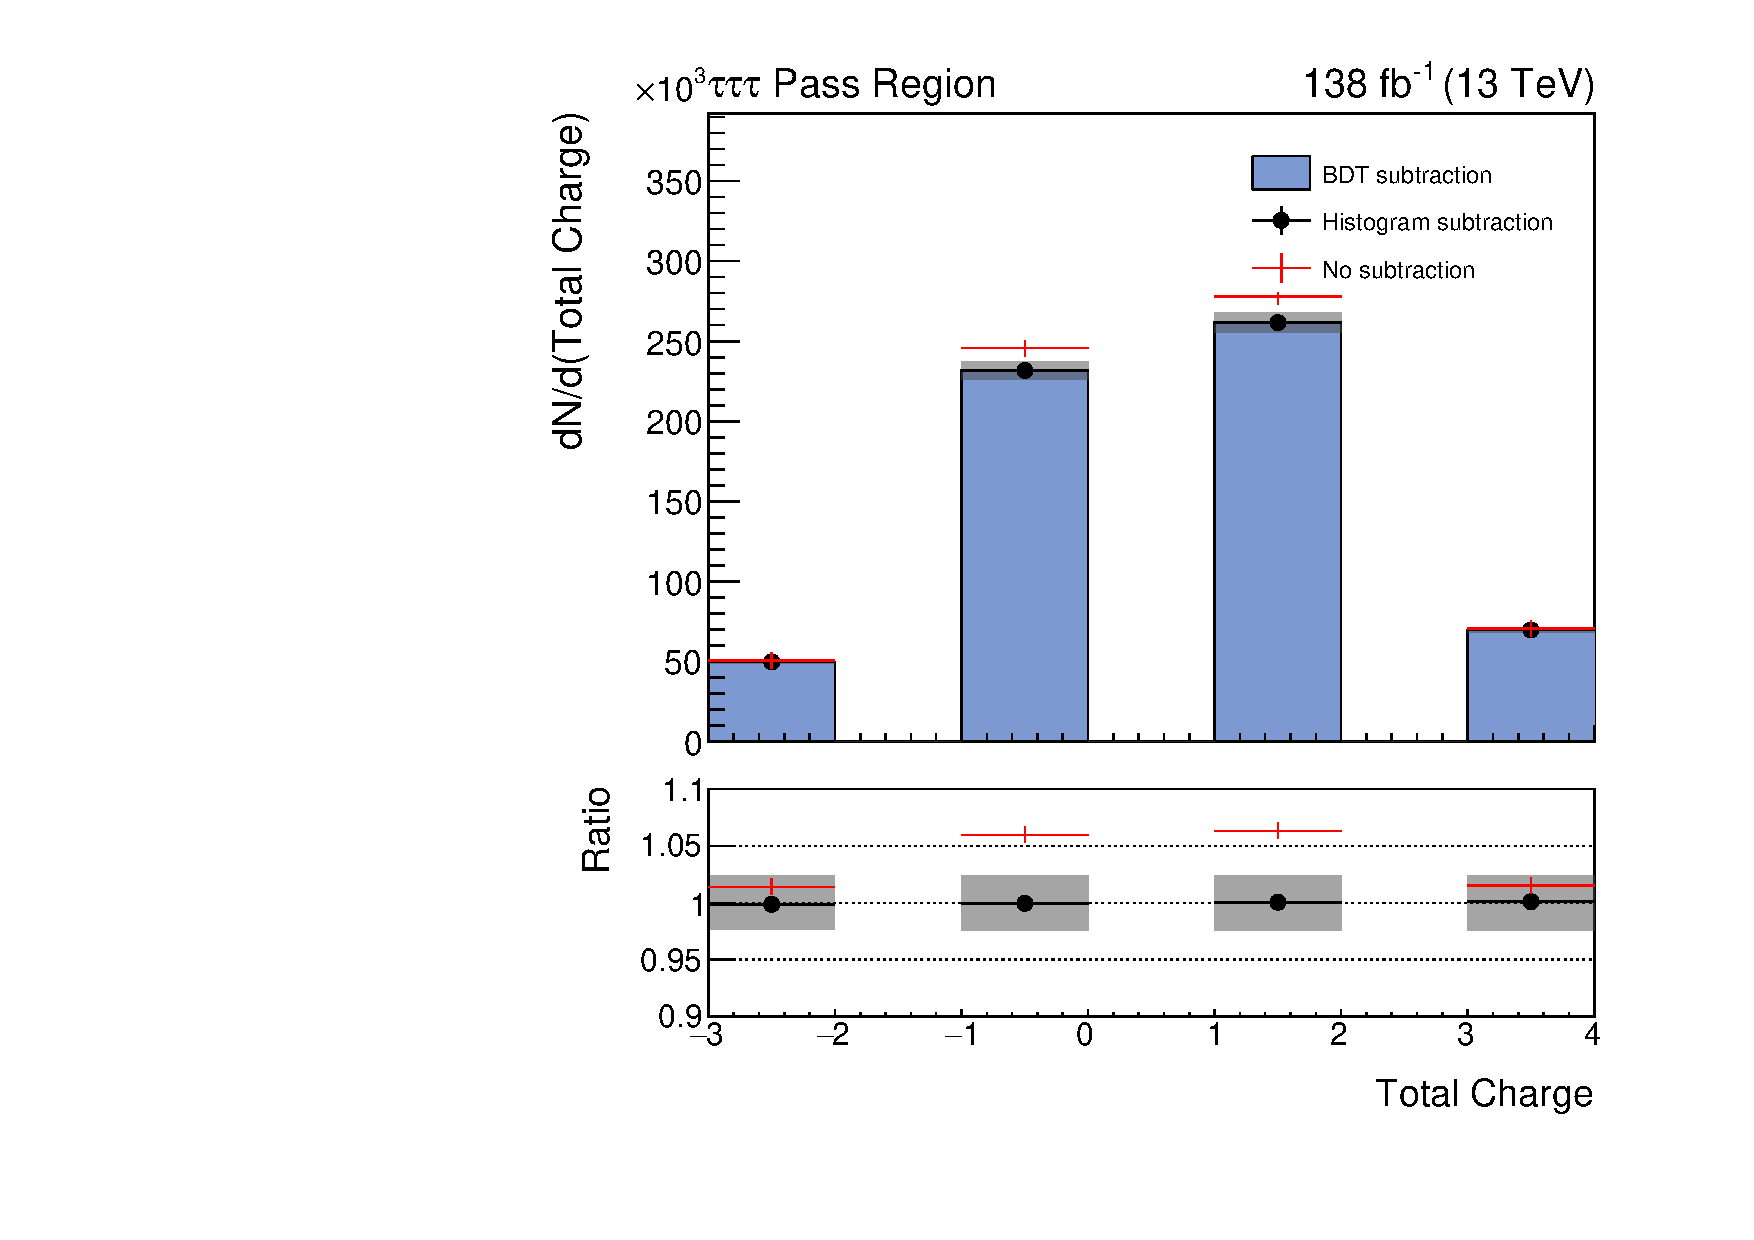
\includegraphics[width=\textwidth]{Figures/Chapter6/subtraction_plot_q_sum_ttt_pass.pdf}
            \caption{}
        \end{subfigure}
    \caption[Comparison of subtraction techniques applied to the total charge distribution of $\PGt_h$ candidates.]{Comparison of subtraction techniques applied to the total charge distribution of $\PGt_h$ candidates in the \textbf{(a)} fail and \textbf{(b)} pass regions.}

    \label{Figure:Chapter6_BDTPurificationExample}
\end{figure}

\subsubsection{\texorpdfstring{Application of the $F_F$}{Application of the Fake Factor}}

As discussed in Section~\ref{Section6:Fitting_Parametrisation}, the ML-based method enables the derivation of a $F_{F}^i$, for each $\PGt_h$ candidate $i$ in the event. However, in events containing multiple $\PGt_h$ candidates, care must be taken to account for all possible misidentification combinations without introducing overcounting. For example, applying $F_{F}^1$ only to the leading candidate neglects subleading misidentified contributions, while applying all $F_{F}^i$ simultaneously results in double-counting. To resolve this, additive and subtractive combinations of the $F_{F}^i$ are used to properly model the full jet$\to\PGt_h$ background. The application logic for events with two and three $\PGt_h$ candidates is summarised in Tables~\ref{Table:Chapter_6_FFApplication_2Taus} and~\ref{Table:Chapter_6_FFApplication_3Taus}, respectively.

\begin{table}[!htbp]
\centering
\renewcommand{\arraystretch}{1.5} % Increase row height
\setlength{\tabcolsep}{12pt} % Increase column width
\arrayrulecolor{black} % Ensure outer border is black
\begin{tabular}{cccc}
\hline
Region & $\PGt_h^1$ \textcolor{red}{$\PGt_h^2$} & \textcolor{red}{$\PGt_h^1$} $\PGt_h^2$ & \textcolor{red}{$\PGt_h^1 \PGt_h^2$} \\ \hline

$F_F^1$ & 0 & 1 & 1 \\
\arrayrulecolor{lightgray} \hline

$F_F^2$ & 1 & 0 & 1 \\
\arrayrulecolor{lightgray} \hline

$-F_F^1 \times F_F^2$ & 0 & 0 & 1 \\
\arrayrulecolor{black} \hline
Combined & 1 & 1 & 1 \\
\end{tabular}
\caption[Combinatorial application of Fake Factors for two $\PGt_h$ candidates.]{
Combinatorial application of $F_F^i$ in events with two $\PGt_h$ candidates. Each column represents a control region where different combinations of candidates are treated as misidentified jets (shown in red). For example, $\PGt_h$\textcolor{red}{$\PGt_h$} indicates a region where the second candidate is assumed to be misidentified.}
\label{Table:Chapter_6_FFApplication_2Taus}
\end{table}


\begin{table}[!htbp]
\centering
\renewcommand{\arraystretch}{1.5} % Increase row height
\setlength{\tabcolsep}{10pt} % Increase column width
\arrayrulecolor{black} % Ensure outer border is black
\begin{tabular}{ccccccc}
\hline
Region & \textcolor{red}{$\PGt_h^1$} $\PGt_h^2$ $\PGt_h^3$ & \textcolor{red}{$\PGt_h^1 \PGt_h^2$} $\PGt_h^3$ & \textcolor{red}{$\PGt_h^1 \PGt_h^2 \PGt_h^3$} & $\PGt_h^1$ \textcolor{red}{$\PGt_h^2 \PGt_h^3$} & $\PGt_h^1$ \textcolor{red}{$\PGt_h^2$} $\PGt_h^3$ & \textcolor{red}{$\PGt_h^1$} $\PGt_h^2$ \textcolor{red}{$\PGt_h^3$} \\ \hline

$F_F^1$ & 1 & 1 & 1 & 0 & 0 & 1 \\
\arrayrulecolor{lightgray} \hline

$F_F^2$ & 0 & 1 & 1 & 1 & 1 & 0 \\
\arrayrulecolor{lightgray} \hline

$F_F^3$ & 0 & 0 & 1 & 1 & 0 & 1 \\
\arrayrulecolor{lightgray} \hline

$-F_F^1 \times F_F^2$ & 0 & 1 & 1 & 0 & 0 & 0 \\
\arrayrulecolor{lightgray} \hline

$-F_F^1 \times F_F^3$ & 0 & 0 & 1 & 0 & 0 & 1 \\
\arrayrulecolor{lightgray} \hline

$-F_F^2 \times F_F^3$ & 0 & 0 & 1 & 1 & 0 & 0 \\
\arrayrulecolor{lightgray} \hline

$F_F^1 \times F_F^2 \times F_F^3$ & 0 & 0 & 1 & 0 & 0 & 0 \\
\arrayrulecolor{black} \hline

Combined & 1 & 1 & 1 & 1 & 1 & 1 \\
\end{tabular}
\caption[Combinatorial application of Fake Factors for three $\PGt_h$ candidates.]{
Combinatorial application of $F_F^i$ in events with three $\PGt_h$ candidates. Each column represents a control region where different combinations of candidates are treated as misidentified jets (shown in red).}
\label{Table:Chapter_6_FFApplication_3Taus}
\end{table}

This approach provides a consistent and statistically robust means of estimating the jet$\to\PGt_h$ background across all final states. By leveraging high-dimensional ML-based reweighting and explicitly accounting for all misidentification combinations through additive and subtractive combinations of $F_F^i$, the method overcomes the key limitations of classical $F_F$ techniques. As such, it forms a central component of the background modelling strategy employed in this analysis.

\section{Uncertainty model}
\label{Section:Chapter6_Uncertainty_Model}

To account for statistical fluctuations arising from the finite size of the simulated signal and background samples, the Barlow–Beeston "lite" method is used~\cite{BARLOW1993219,Conway:2011in}. This method introduces per-bin uncertainties on the predicted yields, ensuring a correct treatment of statistical limitations in the MC templates. n addition to statistical uncertainties, two main categories of systematic uncertainties are included in the model: 

\begin{enumerate}[label=(\roman*)]

\item \textbf{Normalisation}: Only affect the overall event yields

\item \textbf{Shape}: Alter both the yield and shape of the distributions

\end{enumerate}

A summary of the systematic uncertainties considered in this analysis is presented below.

\subsection{Luminosity}

The uncertainty in the integrated luminosity is treated as a normalisation-only uncertainty, affecting the overall yield of simulated samples. It is assumed to be uncorrelated across data-taking years. The assigned uncertainties, based on dedicated luminosity measurements and data-simulation comparisons, are:

\begin{itemize}
    \item 1.2\% for 2016
    \item 2.3\% for 2017
    \item 2.5\% for 2018
\end{itemize}

\subsection{Electron and muon efficiencies}

Uncertainties associated with the reconstruction and selection of light leptons are derived from the tag-and-probe studies discussed in Section~\ref{Section:Chapter6_LightLepton_Corrections}. Two sources of uncertainty are considered:

\begin{enumerate}[label=(\roman*)]
\item \textbf{Identification and Isolation}: \\
A 2\% uncertainty is applied to account for residual variations in the corresponding SFs, due to modelling choices in the tag-and-probe procedure (\eg, tag selection, background and signal parameterisation). Though conceptually a normalisation uncertainty, it is implemented as a shape uncertainty to reflect the kinematic dependence of the SFs across $p_{\mathrm{T}}$ and $\eta$.

\item \textbf{Trigger}: \\
A separate 2\% uncertainty accounts for lepton trigger efficiencies. It is also implemented as a shape uncertainty and applied only to events selected via single-lepton triggers.

\end{enumerate}

\subsection{Hadronic tau efficiencies}

Uncertainties associated with $\PGt_h$ identification and energy scale SFs include:

\begin{enumerate}[label=(\roman*)]
\item \textbf{Statistical components}, arising from the fit parameters, decorrelated by DM and data-taking year.

\item \textbf{Systematic components} split as follows:
\begin{enumerate}
    \item One fully correlated across years and DMs
    \item One correlated across years but decorrelated by DM
    \item One decorrelated across both dimensions
\end{enumerate}
\end{enumerate}

All $\tauh$ uncertainties are implemented as shape variations to capture their dependence on tau kinematics and DM. Additionally, uncertainties in the Double-Tau trigger efficiency are treated as shape uncertainties, correlated across channels and years but decorrelated by DM.

\subsection{Lepton misidentification rates and energy scale}

Uncertainties associated with electrons and muons misidentified as $\tauh$ candidates are treated as shape uncertainties and parameterised as functions of the $p_{\mathrm{T}}$ of the misidentified lepton. 

\begin{itemize}
    \item For muons misidentified as $\tauh$, a flat 1.0\% uncertainty is applied across all data-taking years.
    \item For electrons misidentified as $\tauh$, the uncertainty ranges between 0.5\% and 6.6\%, depending on $p_{\mathrm{T}}$ and $\eta$.
\end{itemize}

These uncertainties are applied as shape variations to account for the dependence on the underlying lepton kinematics.

\subsection{Jet energy scale and resolution}

Systematic uncertainties associated with jets arise from:
\begin{enumerate}[label=(\roman*)]

\item \textbf{Jet Energy Scale}: \\
Evaluated by varying the reconstructed jet energy up and down by $\pm1\sigma$.

\item \textbf{Jet Energy Resolution}: \\
Estimated by smearing the jet momenta in simulation to match the resolution observed in data.

\end{enumerate}

Both JES and JER uncertainties are treated as shape uncertainties. Additionally, an uncertainty is included for the energy scale of the unclustered component of $\vec{E}_\mathrm{T}^{\text{miss,PF}}$\footnote{Unclustered energy refers to PF objects not clustered into jets or associated to leptons.}.

\subsection{Prefiring}
The prefiring uncertainty accounts for the incorrect identification of the bunch crossing by the Level-1 trigger, primarily due to ECAL endcap misalignments in 2016 and 2017 data. Event-by-event prefiring weights are applied to simulated events based on jet and photon kinematics. The uncertainty associated with these weights is implemented as a shape variation, decorrelated by year.

\subsection{B-tagging efficiencies}
Uncertainties associated with the b-tagging efficiency corrections are parameterised as functions of jet $p_{\text{T}}$ and $\eta$. These uncertainties are propagated by varying the corresponding b-tagging scale factors within their prescribed uncertainties. The resulting impact on event yields typically ranges from 0\% to 3\%.

\subsection{Theoretical Uncertainties on \texorpdfstring{$\PZ\PZ \rightarrow 4\ell$}{ZZ → 4l} Samples}

The $\PZ\PZ \rightarrow 4\ell$ background is affected by higher-order theoretical corrections. A dedicated uncertainty is assigned by comparing the yield obtained with the $k$-factor applied twice to that obtained with no $k$-factor applied. The resulting variation is treated as a normalisation uncertainty. This uncertainty is applied to all relevant samples and considered correlated across channels and years.

\subsection{Signal theory uncertainties}

Uncertainties related to the theoretical modelling of the signal include:

\begin{itemize}
    \item \textbf{PDFs}: A 6\% normalisation uncertainty, derived from the envelope of PDF variations.
    \item \textbf{$\alpha_s$}: A 1\% normalisation uncertainty.
    \item \textbf{Renormalisation and factorisation scales ($\mu_R$, $\mu_F$)}: A 2\% uncertainty, reflecting yield variations under scale variations.
\end{itemize}

\subsection{Jets \texorpdfstring{$\to \PGt_h$}{to hadronic tau} background}

Multiple sources of uncertainty are associated with the ML-based $F_F$ method. These uncertainties are treated as uncorrelated across final states, with the exception of the $\tauh\tauh\tauh\tauh$ and $\tauh\tauh\tauh$ channels, where the same ML FF fit is used. The main sources of uncertainty are summarised below:

\begin{itemize}
    \item \textbf{Contamination from non-jet backgrounds in the fit region:}
    \begin{itemize}
        \item \textit{BDT subtraction:} An uncertainty is assigned by comparing the variable distributions obtained using standard histogram subtraction and those obtained with the BDT-based subtraction. The largest observed deviation in each variable is taken as the systematic uncertainty. This comparison is performed separately in the pass and fail $\tauh$ identification regions.
        \item \textit{MC mismodelling of non-jet contributions:} To account for uncertainties in the simulation of non-jet $\rightarrow \tauh$ objects, the MC contributions are varied by $\pm$10\%. The BDT subtraction and $F_F$ procedures are repeated using the varied samples, and the resulting changes are taken as systematic uncertainties.
    \end{itemize}

    \item \textbf{BDT $F_F$ fit:}
    \begin{itemize}
        \item \textit{Fit closure:} An uncertainty is derived by comparing the reweighted distributions in the fail $\tauh$ identification region to those in the pass region. Any observed non-closure is propagated as a systematic uncertainty.
        \item \textit{Sideband variable dependence:} An uncertainty is placed to cover any potential dependency of the $F_F$ on the choice of sideband variables. To quantify this, alternative sideband variable combinations are used in the fit. The largest resulting deviation is taken as the uncertainty and is decorrelated across each variable combination.
    \end{itemize}
\end{itemize}

\section{Search strategy and statistical procedure}








\setcounter{mtc}{7}
\chapter{\texorpdfstring{Measuring the CP structure of the Higgs-tau Yukawa coupling in $\PGt_h \PGt_h$ decays}{Measurement of the CP structure of the Higgs-tau Yukawa coupling in tauh tauh decays}}
\chaptermark{Measurement of Higgs CP structure in \texorpdfstring{$\PH\to\tau_h\tau_h$}{H tau tau} decays}
\thispagestyle{plain}  % First page has default style
\pagestyle{chapterpages}
\label{Section:Chapter_CP}
\minitoc

\section{Introduction}
\label{Section:Chapter7_Introduction}
As outlined in Section~\ref{Section:Chapter2_CP_Yukawa_Structure}, the CP structure of the $\PH\tau\tau$ Yukawa coupling can be probed through spin correlations in $H \to \tau\tau$ decays. These correlations are captured in the acoplanarity angle $\phi_{CP}$ between the $\tau^+$ and $\tau^-$ decay planes, which serves as the primary CP-sensitive observable.

In the \ac{SM}, this measurement is expressed in terms of the effective CP mixing angle $\alpha^{\PH\tau\tau}$ (defined in Section~\ref{Section:Chapter2_HiggsCPStructurethroughHttdecays}), which is predicted to be essentially zero for a purely CP-even interaction. A significant deviation of $\alpha^{\PH\tau\tau}$ from zero would constitute direct evidence for CP violation in the Higgs--fermion sector, with important implications for physics beyond the \ac{SM}. Minimal supersymmetric models predict only negligible CP-violating effects in Yukawa couplings, whereas extended Higgs sectors such as the next-to-minimal supersymmetric model can accommodate values up to ${\sim}27^\circ$~\cite{King:2015oxa}.

The most precise determination to date was performed by the \ac{CMS} Collaboration using the full Run~2 dataset of $137~\mathrm{fb}^{-1}$ at $\sqrt{s} = 13~\mathrm{TeV}$~\cite{HiggsCP_CMS_2021}. That analysis combined multiple $\tau$ decay channels, including leptonic modes ($\tau_e^\pm,\ \tau_\mu^\pm$) and the dominant hadronic modes ($\pi^\pm$, $\rho^\pm \to \pi^\pm \pi^0$, $a_1^\pm \to \pi^\pm \pi^0 \pi^0$, $a_1^\pm \to \pi^\pm \pi^\mp \pi^\pm$). The result, $\alpha^{\PH\tau\tau} = -1 \pm 19^\circ$, with an expected precision of $0 \pm 21^\circ$ at 68.3\%~CL, disfavors the pure CP-odd scenario at the $3.0\sigma$ level. The measurement remains dominated by statistical uncertainty. Feasibility studies indicate that a precision of ${\sim}5$-$10^\circ$ could be achieved with $3\unit{ab}^{-1}$ of data~\cite{Harnik:2013aja,Berge:2014sra}.

This chapter presents a complementary measurement focusing exclusively on the $\PGt_h \PGt_h$ final state. The dataset corresponds to the partial Run 3 data-taking period and is substantially smaller in integrated luminosity than that used in Run 2, limiting the statistical reach. Nevertheless, this analysis aims to approach the precision of the Run~2 results by implementing improvements in key components, including:

\begin{enumerate}[label=(\roman*)]
    \item Tau Identification
    \item Triggering
    \item Tau \ac{DM} Classification
    \item Event Categorisation
    \item Reconstruction of the CP-sensitive observable
\end{enumerate}

These developments are intended to pave the way for a competitive measurement well before the \ac{HL}-\ac{LHC} era. The following sections discuss these aspects in more detail, together with the improved analysis strategy.


\section{Collision data}

This analysis uses pp collision data recorded by the \ac{CMS} detector during the initial part of the Run 3 data-taking period (2022–2023). The collisions were produced at a centre-of-mass energy of $\sqrt{s} = 13.6\TeV$, and the dataset corresponds to an integrated luminosity of about $62.4\unit{fb}^{-1}$.

\section{Backgrounds}
\label{Section:Chapter7_Backgrounds}

Many of the background processes relevant to the fully hadronic ditau ($\PGt_h\PGt_h$) final state are the same as those discussed for the four-tau analysis in Section~\ref{Section:Chapter6_Backgrounds}. The main difference is that the selection here requires only two reconstructed tau candidates, both hadronically decaying. Events can therefore enter the signal region through three main mechanisms:  
\begin{enumerate}[label=(\roman*)]
    \item Events with two genuine $\PGt_h$ leptons  
    \item Events with one genuine $\PGt_h$ and one misidentified object (jet or prompt electron/muon reconstructed as $\PGt_h$)  
    \item Events with two misidentified objects, typically jets or nonprompt electrons/muons, both reconstructed as $\PGt_h$
\end{enumerate}

Compared to the four-tau case, both the composition and ranking of backgrounds change noticeably. \textbf{\ac{DY}} ($\PZ/\gamma^*\to\PGt^+\PGt^-$) with both taus decaying hadronically is now the dominant source of genuine $\PGt_h\PGt_h$ pairs. \textbf{Top-quark pair production} ($\ttbar$) also makes a large contribution, both through $\PW\to\PGt\nu_\PGt$ decays (genuine $\PGt_h$) and through the misidentification of jets or prompt leptons as $\PGt_h$, with the associated $b$-jets increasing the likelihood of additional jet activity. Backgrounds from \textbf{$\PW$+jets} and \textbf{\ac{QCD}-induced multijet production} are also significant, as only one or two jet$\to\PGt_h$ (or $e/\mu\to\PGt_h$) misidentifications are needed to pass the $\PGt_h\PGt_h$ selection.  

In contrast to the four-tau analysis, where \textbf{$ZZ\to4\PGt$} was the most important irreducible background, $ZZ$ production is subdominant here. This is because events with four taus rarely pass the $\PGt_h\PGt_h$ selection unless two of the taus are outside the detector acceptance or fail identification. Other processes, such as triboson and single-top production, contribute only subdominantly.  

The modelling and estimation strategies for these background contributions, including the treatment of jet and lepton misidentification, are detailed in Section~\ref{Section:Chapter7_Background_Modelling}. The full list of simulated background processes is broadly similar to that presented for the four-tau analysis in Table~\ref{Table:Chapter6_SimulatedBackgrounds}, and is reproduced here in Table~\ref{Table:Chapter7_SimulatedBackgrounds} for completeness.

{
\centering
\setlength{\LTpost}{-2ex}  % tighten space after table
\small  % one size smaller than normal
\begin{longtable}{llc}
\caption[Summary of simulated Standard Model backgrounds for the $H \to \PGt_h\PGt_h$ CP measurement.]
{Summary of the simulated \ac{SM} background processes used in the measurement of the CP structure of the Higgs–tau Yukawa coupling in $H \to \PGt_h\PGt_h$ decays, listing the event generators and the theoretical precision of their cross sections.}

\label{Table:Chapter7_SimulatedBackgrounds} \\
\hline
\textbf{Process} & \textbf{Generators} & \textbf{Cross section $\sigma$ [pb]} \\
\hline \hline
\endfirsthead

\hline
\textbf{Process} & \textbf{Generators} & \textbf{Cross section $\sigma$ [pb]} \\
\hline \hline
\endhead

\hline
\multicolumn{3}{r}{\textit{Continued on next page}} \\
\endfoot

\hline
\endlastfoot
\rowcolor{verylightblue}
\textbf{\ac{DY}, $\PZ/\gamma^* \to \ell^+ \ell^-$ (\ac{NLO})} & & \\
+1 jets\hyperlink{DY_FxFx}{$^1$}, $m_{\ell \ell} > 50\GeV$ & \MCATNLO, \PYTHIA & 1788.0 (\ac{NLO}) \\
+2 jets\hyperlink{DY_FxFx}{$^1$}, $m_{\ell \ell} > 50\GeV$ & \MCATNLO, \PYTHIA & 339.6 (\ac{NLO})\\
+3 jets\hyperlink{DY_FxFx}{$^1$}, $m_{\ell \ell} > 50\GeV$ & \MCATNLO, \PYTHIA & 125.1 (\ac{NLO}) \\

\arrayrulecolor{lightgray}\hline
\rowcolor{verylightblue}
\textbf{W+jets (\ac{LO})} & & \\
+ jets & \MADGRAPH, \PYTHIA & 55300.0 (\ac{LO}), 63425.1 (\ac{NLO}\hyperlink{Higher-Order-XS}{$^2$}) \\
+1 jets & \MADGRAPH, \PYTHIA & 9128.0 (\ac{LO}) \\
+2 jets & \MADGRAPH, \PYTHIA & 2922.0 (\ac{LO}) \\
+3 jets & \MADGRAPH, \PYTHIA & 861.3 (\ac{LO}) \\
+4 jets & \MADGRAPH, \PYTHIA & 415.4 (\ac{LO}) \\

\arrayrulecolor{lightgray}\hline
\rowcolor{verylightblue}
\textbf{\ttbar (\ac{NLO})} & & \\
Fully hadronic & \POWHEG, \PYTHIA & 419.81 (\ac{NNLO}\hyperlink{Higher-Order-XS}{$^2$})\\
Semi-leptonic & \POWHEG, \PYTHIA & 405.75 (\ac{NNLO}\hyperlink{Higher-Order-XS}{$^2$})\\
Fully leptonic & \POWHEG, \PYTHIA & 98.04 (\ac{NNLO}\hyperlink{Higher-Order-XS}{$^2$}) \\

\arrayrulecolor{lightgray}\hline
\rowcolor{verylightblue}
\textbf{Single top (\ac{NLO})} & & \\
t-channel ($t$) & \POWHEG, \PYTHIA & 145.0 (\ac{NNLO}\hyperlink{Higher-Order-XS}{$^2$}) \\
t-channel ($\overline{t}$) & \POWHEG, \PYTHIA & 87.2 (\ac{NNLO}\hyperlink{Higher-Order-XS}{$^2$}) \\
$t + W^-$ & \POWHEG, \PYTHIA & 43.95 (\ac{NNLO}\hyperlink{Higher-Order-XS}{$^2$}) \\
$t + W^+$ & \POWHEG, \PYTHIA & 43.95 (\ac{NNLO}\hyperlink{Higher-Order-XS}{$^2$}) \\

\arrayrulecolor{lightgray}\hline
\rowcolor{verylightblue}
\textbf{Diboson (\ac{LO})} & & \\
$\PW \PZ$  & \PYTHIA & 44.35 (\ac{NNLO}\hyperlink{Higher-Order-XS}{$^2$}) \\
$\PW \PW$  & \PYTHIA & 122.27 (\ac{NNLO}\hyperlink{Higher-Order-XS}{$^2$}) \\
$\PZ \PZ$  & \PYTHIA & 19.43 (\ac{NNLO}\hyperlink{Higher-Order-XS}{$^2$}) \\

\arrayrulecolor{lightgray}\hline
\rowcolor{verylightblue}
\textbf{Triboson (\ac{NLO})} & & \\
$\PW \PW \PZ $ & \MCATNLO, \PYTHIA & 0.1851 (\ac{NLO})\\
$\PW \PZ \PZ $ & \MCATNLO, \PYTHIA & 0.0621 (\ac{NLO})\\
$\PW \PW \PW $ & \MCATNLO, \PYTHIA & 0.2328 (\ac{NLO})\\
$\PZ \PZ \PZ $ & \MCATNLO, \PYTHIA & 0.0159 (\ac{NLO})\\

\arrayrulecolor{black}\hline
\end{longtable}
}
\vspace{0.5em}
\noindent\begin{minipage}{\linewidth}
\footnotesize
\hypertarget{DY_FxFx}{}$^{1}$For the \ac{DY} samples, only exclusive jet multiplicity samples are generated at \ac{NLO} using the FxFx jet merging scheme~\cite{FxFx}. No inclusive sample is produced in this case.\\
\hypertarget{Higher-Order-XS}{}$^{2}$While the samples are generated at the perturbative order indicated by the generator, the normalisation is performed using the best available cross sections.
\end{minipage}

\section{Modelling of signal processes}
\label{Section:Chapter7_SignalModelling}

The signal samples used in this analysis correspond to Higgs boson production through \ac{ggH}, \ac{VBF}, and \ac{VH} ($\PW\PH$, $\PZ\PH$). All samples are generated with the \POWHEG v2.0 event generator~\cite{Powheg_0,Powheg_1,Powheg_2,Powheg_3}. To ensure that the measurement of $\alpha^{\PH\tau\tau}$ remains unbiased with respect to the Higgs boson production CP structure, the event selection and categorisation were designed without relying on observables directly sensitive to production CP properties. In particular, variables such as the azimuthal separation between the two leading jets were deliberately not included.

As with background samples discussed in Section~\ref{Section:Chapter7_Backgrounds}, the $\PGt$ decays are simulated with \PYTHIA (version 8.230)~\cite{PYTHIA}. In the initial simulation, the spins of the $\tau$ pair are uncorrelated. The proper spin correlations, which encode the CP-sensitive effects of the $\PH \to \tau\tau$ interaction, are subsequently incorporated through reweighting with the \TAUSPINNER package~\cite{Przedzinski:2018ett}. This tool computes per-event weights corresponding to benchmark CP scenarios:

\begin{itemize}
    \item Pure CP-even ($\alpha^{\PH\tau\tau} = 0^\circ$) 
    \item Pure CP-odd ($\alpha^{\PH\tau\tau} = 90^\circ$) 
    \item Maximally mixed ($\alpha^{\PH\tau\tau} = 45^\circ$) 
\end{itemize}  

These per-event weights enable the construction of differential distributions at arbitrary values of the effective mixing angle through linear combinations of the benchmark templates. In practice, this is achieved using the decomposition:    

\begin{equation_pad}
\begin{aligned}
    \frac{d\sigma}{dx}(\alpha^{\PH\tau\tau}) 
    &= (\cos^2\alpha^{\PH\tau\tau} - \cos\alpha^{\PH\tau\tau}\sin\alpha^{\PH\tau\tau})  \frac{d\sigma}{dx}\Big|_{\text{CP-even}} \\
    &+ (\sin^2\alpha^{\PH\tau\tau} - \cos\alpha^{\PH\tau\tau}\sin\alpha^{\PH\tau\tau})  \frac{d\sigma}{dx}\Big|_{\text{CP-odd}}\\
    &+ 2\cos\alpha^{\PH\tau\tau}\sin\alpha^{\PH\tau\tau} \, \frac{d\sigma}{dx}\Big|_{\text{CP-mix}}
\end{aligned}
\end{equation_pad} 

All acoplanarity angle distributions presented in this chapter include a ``Nominal'' curve, which corresponds to the unweighted sample (\ie with the CP benchmark reweighting factor set to unity).

\section{Reconstruction of \texorpdfstring{$\phi_{CP}$}{phiCP}}
\label{Section:Chapter7_PhiCP_Reconstruction}
As discussed in Section~\ref{Section:Chapter2_HiggsCPStructurethroughHttdecays}, $\phi_{CP}$ is formally defined through the \acp{P.V.} of the two $\tau$ leptons. In the Higgs boson rest frame, this construction provides the optimal estimator of the $\tau$ spin correlations and therefore of the CP structure of the $\PH\tau\tau$ interaction. 

Experimentally, a full reconstruction of the \ac{P.V.} is rarely possible. Because most $\tau$ decays involve one or more neutrinos whose momenta cannot be reconstructed, the $\tau$ rest frames are not directly accessible. As a result, direct access to the Higgs rest frame is limited to only a subset of \acp{DM}. To overcome these challenges, alternative reconstruction frames and methods have been developed. 

To make the measurement experimentally accessible, $\phi_{CP}$ is reconstructed in the \ac{ZMF} of two visible $\tau$ decay products. This works because
the polarisation of each $\tau$ lepton is transferred to the angular
distributions of its decay products. In other words, the visible products retain
information about the parent $\tau$ spins, so the decay planes reconstructed from these products inherit the spin correlations. Therefore, their relative orientation continues to encode the CP properties of the $\PH\tau\tau$ coupling. 

In the remainder of this section, the different reconstruction strategies employed are described in more detail. Throughout, the symbol $\phi_{CP}$ is used generically to denote the reconstructed acoplanarity angle, irrespective of the specific method chosen.

\subsection{Impact parameter method}
\label{Section:Chapter7_IP_METHOD}
The \ac{IP} method exploits the finite lifetime of $\tau$ leptons to approximate their decay planes using tracking information. This method provides the highest CP sensitivity when both taus decay into a single charged particle. A schematic of this method is shown in Fig.~\ref{Figure:Chapter7_IP_IP_Method}.

\begin{figure}[!htbp]
    \centering
    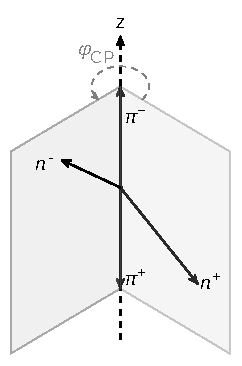
\includegraphics[width=0.4\textwidth]{Figures/Chapter7/Acoplanarity/Diagrams/IP-IP.pdf}
    \caption[Acoplanarity angle $\phi_{CP}$ reconstructed in the $\tauh\tauh \to \pi\pi$ category using the impact parameter method.]
    {Acoplanarity angle $\phi_{CP}$ reconstructed in the $\tauh\tauh \to \pi\pi$ category using the \ac{IP} method.}
    \label{Figure:Chapter7_IP_IP_Method}
\end{figure}

The method reconstructs each $\tau$ decay plane from the spatial momentum of the charged decay product ($\mathbf{q^\pm}$) together with its associated \ac{IP} vector ($\mathbf{n^\pm}$), as defined in Section~\ref{Section:Chapter4_Vertex_reconstruction}. These are expressed as four-vectors: the four-momentum of the charged particle $q^\pm$ and the impact-parameter four-vector $n^\pm = (0,\mathbf{n^\pm})$, both measured in the laboratory frame. The set of four-vectors is then boosted into the rest frame of the two charged particles, \ie the visible ditau \ac{ZMF} (denoted by $_\text{ZMF}$). In the \ac{ZMF}, the boosted \ac{IP} three-vector is normalised and decomposed into components parallel and transverse to the corresponding normalised three-momentum vector of the charged particle. From these, two key observables are defined: $\phi_{\text{ZMF}}$ and $O_{\text{ZMF}}$\footnote{The observable $O_{\text{ZMF}}$ resolves the twofold ambiguity in the angle between decay planes, which would otherwise be confined to the interval $[0,\pi]$. Its sign encodes the relative orientation (clockwise or anticlockwise) of the planes, thereby unfolding the acoplanarity angle to the full range $[0,2\pi]$ and retaining sensitivity to the CP phase of the $\PH\tau\tau$ coupling.}.
\begin{equation_pad}
    \phi_{\text{ZMF}} = \arccos(\hat{\mathbf{n}}_{\text{ZMF},\perp}^{+} \, \, \cdot \, \, \hat{\mathbf{n}}_{\text{ZMF},\perp}^{-})
\end{equation_pad}
\begin{equation_pad}
    O_{\text{ZMF}} = \hat{\mathbf{q}}^-_\text{ZMF} \, \, \cdot \, \,(\hat{\mathbf{n}}_{\text{ZMF},\perp}^{+} \, \, \times \, \, \hat{\mathbf{n}}_{\text{ZMF},\perp}^{-})
\end{equation_pad}

The acoplanarity angle is then defined over the full range $[0,2\pi]$ by:

\begin{equation_pad}
\phi_{CP} \;=\;
\begin{cases}
\phi_{\text{ZMF}} & O_{\text{ZMF}} \ge 0 \\
2\pi - \phi_{\text{ZMF}} & O_{\text{ZMF}} < 0
\end{cases}
\end{equation_pad}

The performance of the \ac{IP} method is illustrated by the reconstructed $\phi_{CP}$ distribution in the $\pi\pi$ category, shown in Fig.~\ref{Figure:CPDist_IPMethod_pipi}.

\begin{figure}[!htbp]
    \centering
    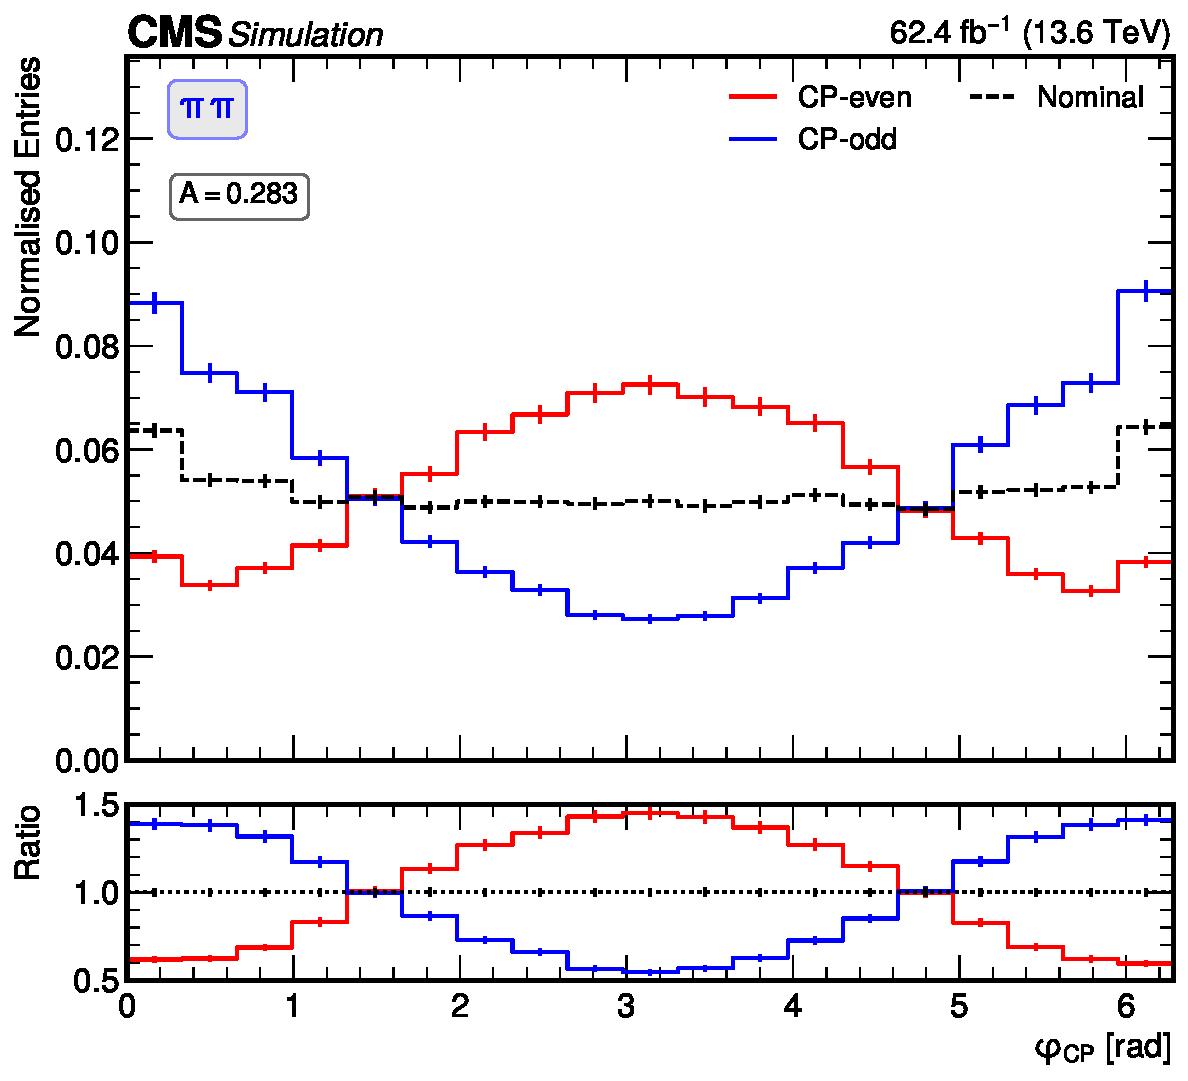
\includegraphics[width=0.6\textwidth]{Figures/Chapter7/Acoplanarity/With_IP/aco_pi_pi.pdf}
    \caption[Reconstructed $\phi_{CP}$ distribution in the $\tauh\tauh \to \pi\pi$ category using the impact parameter method.]
    {Reconstructed distribution of the acoplanarity angle $\phi_{CP}$ in the $\tauh\tauh \to \pi\pi$ category, obtained with the \ac{IP} method. The plots are obtained from the signal samples used in this analysis.}
    \label{Figure:CPDist_IPMethod_pipi}
\end{figure}

\subsection{Neutral-pion method}
\label{Section:NeutralPionMethod}

The \ac{NP} method, also referred to as the \textit{decay-plane method}, is designed for $\tau$ decays via the $\rho^\pm$ resonance, \ie $\tau^\pm \to \rho^\pm \nu_\tau$ with $\rho^\pm \to \pi^\pm \pi^0$. A schematic illustration of this method is shown in Fig.~\ref{Figure:Chapter7_NP_Method}. In this case, the $\tau$ decay plane is reconstructed from the momentum vectors of the charged pion ($\mathbf{q^\pm}$) and the neutral pion ($\mathbf{q^{0\pm}}$). Here, the neutral pion provides the secondary axis defining the plane, replacing the \ac{IP} vector used in the \ac{IP} method (Section~\ref{Section:Chapter7_IP_METHOD}).  

\begin{figure}[!htbp]
    \centering
    \includegraphics[width=0.4\textwidth]{Figures/Chapter7/Acoplanarity/Diagrams/NP-NP.pdf}
    \caption[Acoplanarity angle $\phi_{CP}$ reconstructed in the $\tauh\tauh \to \rho\rho$ category using the neutral-pion method.]
    {Acoplanarity angle $\phi_{CP}$ reconstructed in the $\tauh\tauh \to \rho\rho$ category using the \ac{NP} method.}
    \label{Figure:Chapter7_NP_Method}
\end{figure}

In analogy with the IP construction, the acoplanarity angle is first defined as,

\begin{equation_pad}
    \phi_{\text{ZMF}} = \arccos(\hat{\mathbf{q}}^{0+}_{\text{ZMF},\perp} \cdot \hat{\mathbf{q}}^{0-}_{\text{ZMF},\perp}),
\end{equation_pad}

where the transverse components of the neutral pion momenta are taken with respect to the associated charged-pion directions in the visible ditau \ac{ZMF}. To resolve the twofold ambiguity, a triple product observable is constructed as,

\begin{equation_pad}
    O_{\text{ZMF}} = \hat{\mathbf{q}}^-_{\text{ZMF}} \cdot (\hat{\mathbf{q}}^{0+}_{\text{ZMF},\perp} \times \hat{\mathbf{q}}^{0-}_{\text{ZMF},\perp}),
\end{equation_pad}

and the sign of $O_{\text{ZMF}}$ unfolds the angle to the full $[0,2\pi]$ range, thereby defining $\phi^\prime_{CP}$ as the signed acoplanarity angle:

\begin{equation_pad}
\phi^{\prime}_{CP} =
\begin{cases}
\phi_{\text{ZMF}}, & O_{\text{ZMF}} \ge 0 \\
2\pi - \phi_{\text{ZMF}}, & O_{\text{ZMF}} < 0
\end{cases}
\end{equation_pad}  

An additional refinement, specific to the $\rho$ channel, exploits the \textit{spin-analyser function},

\begin{equation_pad}
    y_\rho^\pm = \frac{E_{\pi^\pm} - E_{\pi^0}}{E_{\pi^\pm} + E_{\pi^0}},
\end{equation_pad}

where $E_{\pi^\pm}$ and $E_{\pi^0}$ are the energies of the charged and neutral pions in the laboratory frame. The product $y_\rho^+ y_\rho^-$ encodes the relative orientation of the spin-analyser vectors for the two $\tau$ decays and enhances the CP sensitivity. The final observable is thus defined as

\begin{equation_pad}
\phi_{CP} =
\begin{cases}
\phi^\prime_{CP}, & y_\rho^+ y_\rho^- \geq 0 \\
\phi^\prime_{CP} + \pi \; \,(\text{mod } 2\pi), & y_\rho^+ y_\rho^- < 0
\end{cases}
\end{equation_pad}

The performance of the \ac{NP} method is demonstrated in Fig.~\ref{Figure:CPDist_NPMethod}, which shows the reconstructed $\phi_{CP}$ distribution for the $\rho\rho$ category.

\begin{figure}[!htbp]
    \centering
    \includegraphics[width=0.6\textwidth]{Figures/Chapter7/Acoplanarity/With_IP/aco_rho_rho.pdf}
    \caption[Reconstructed $\phi_{CP}$ distribution in the $\tauh\tauh\to\rho\rho$ category using the neutral-pion method.]
    {Reconstructed distribution of the acoplanarity angle $\phi_{CP}$ in the $\tauh\tauh \to \rho\rho$ category, obtained with the \ac{NP} method from signal simulation.}
    \label{Figure:CPDist_NPMethod}
\end{figure}

\subsection{Polarimetric vector method in the $a_1^{3\mathrm{pr}}a_1^{3\mathrm{pr}}$ channel}
\label{Section:Chapter7_PV_Method}
The \ac{P.V.} method exploits the fact that, for certain $\tau$ \acp{DM}, the full kinematics of the $\tau$ lepton can be reconstructed with sufficient accuracy. This is the case when both $\tau$ leptons decay via the $a_1^\text{3pr}$ resonance, in which the \acp{SV} can be reconstructed from the three charged tracks of each decay. The $\tau$ lepton momentum direction is taken from the line connecting the \ac{PV} and \ac{SV}. Its magnitude is determined from the two-body decay kinematics $\tau \to a_1\nu_\tau$ under the assumptions of fixed $m_\tau$ and $m_{a_1}$ and a massless neutrino, as follows:

\begin{equation_pad}
|\vec{p}_\tau| = 
\frac{(m_{a_1}^2 + m_\tau^2)\,|\vec{p}_{a_1}| \cos\theta_{\mathrm{GJ}} \;\pm\; 
\sqrt{(m_{a_1}^2 + |\vec{p}_{a_1}|^2)\,\big[(m_{a_1}^2 - m_\tau^2)^2 - 4m_\tau^2 |\vec{p}_{a_1}|^2 \sin^2\theta_{\mathrm{GJ}}\big]}}
{2\,(m_{a_1}^2 + |\vec{p}_{a_1}|^2 \sin^2\theta_{\mathrm{GJ}})}.
\label{Equation:TauPTMag_PV}
\end{equation_pad}

Here $\theta_{\mathrm{GJ}}$ is the Gottfried--Jackson angle~\cite{Cherepanov:2018npf}, defined as the angle between the $\tau$ and $a_1$ momenta in the laboratory frame, and is constrained to lie within a physical maximum $\theta_{\mathrm{GJ}}^{\mathrm{max}}$. In practice, detector resolution effects may lead to $\theta_{\mathrm{GJ}} > \theta_{\mathrm{GJ}}^{\mathrm{max}}$, in which case $\theta_{\mathrm{GJ}}$ is set to $\theta_{\mathrm{GJ}}^{\mathrm{max}}$.  

Equation~\ref{Equation:TauPTMag_PV} admits two possible solutions for the magnitude of the $\tau$ lepton momentum. This ambiguity arises because, in the $\tau$ rest frame, the $a_1$ meson can be emitted either in the same direction as, or opposite to, the $\tau$ momentum in the laboratory frame. The case where the $a_1$ is emitted orthogonally corresponds to the unique solution in which the square root term vanishes. When applied to both $\tau$ decays in an event, this leads in general to up to four candidate solutions for the pair of $\tau$ momenta. The ambiguity is resolved by choosing the solution whose reconstructed ditau mass is closest to the nominal Higgs boson mass.

With the $\tau$ four-momenta determined, the \acp{PV} $\mathbf{h}_1$ and $\mathbf{h}_2$ are computed using the resonance model implemented in \TAUOLA~\cite{Jadach:1990mz,Jezabek:1991qp,Jadach:1993hs}, calibrated with experimental parameters from CLEO~\cite{CLEO:1999rzk}. To build a CP-sensitive observable, $\mathbf{k_{1,2}}$ vectors are defined as,

\begin{equation_pad}
\mathbf{\hat{k}}_{1,2} = \frac{\mathbf{\hat{h}}_{1,2} \times \mathbf{\hat{n}}_{1,2}}{|\mathbf{\hat{h}}_{1,2} \times \mathbf{\hat{n}}_{1,2}|},
\end{equation_pad}

where $\mathbf{\hat{n}}_{1,2}$ denote the unit vectors of the $\tau$ momenta in the Higgs rest frame. From these, the acoplanarity angle $\phi^*$ and the triple product observable $O^*$ are constructed as,  

\begin{equation_pad}
    \phi^* = \arccos(\mathbf{k}_1 \cdot \mathbf{k}_2)
\end{equation_pad}
\begin{equation_pad}
    O^* = - (\mathbf{\hat{h}}_1 \times \mathbf{\hat{h}}_2) \cdot \mathbf{\hat{n}}_1
\end{equation_pad}

with $^*$ denoting quantities in the Higgs rest frame. The final CP-sensitive observable is defined as,

\begin{equation_pad}
\phi_{CP} \;=\;
\begin{cases}
\phi^* & O^* \ge 0 \\
2\pi - \phi^* & O^* < 0
\end{cases}
\end{equation_pad}

An example of the $\phi_{CP}$ distribution reconstructed with the \ac{P.V.} method in the $a_1^{3\mathrm{pr}}a_1^{3\mathrm{pr}}$ category is shown in Fig.~\ref{Figure:CPDist_PVMethod}.

\begin{figure}[!htbp]
    \centering
    \includegraphics[width=0.6\textwidth]{Figures/Chapter7/Acoplanarity/With_IP/aco_a1_a1.pdf}
    \caption[Reconstructed $\phi_{CP}$ distribution in the $\tauh\tauh\to a_1^\text{3pr}a_1^\text{3pr}$ category using the \ac{P.V.} method.]
    {Reconstructed distribution of the acoplanarity angle $\phi_{CP}$ in the $\tauh\tauh \to a_1^\text{3pr}a_1^\text{3pr}$ category, obtained with the \ac{P.V.} method.}
    \label{Figure:CPDist_PVMethod}
\end{figure}

\subsection{Combined methods}
\label{Section:Chapter7_CombinedMethods}

The first combined method utilises both the \ac{IP} and \ac{NP} techniques, applied in channels where the two $\tau$ leptons decay through different modes. In particular, this strategy is relevant in the $\tauh\tauh \to \rho\pi$ category. In such cases, the decay plane of the $\tau_h\to\rho$ is reconstructed with the \ac{NP} method, while the other is reconstructed with the \ac{IP} method. The two planes are then combined in the visible ditau \ac{ZMF} to define $\phi_{CP}$. A schematic illustration of this method is shown in Fig.~\ref{Figure:Chapter7_IPNP_Method}.

\begin{figure}[!htbp]
    \centering
    \includegraphics[width=0.4\textwidth]{Figures/Chapter7/Acoplanarity/Diagrams/IP-NP.pdf}
    \caption[Acoplanarity angle $\phi_{CP}$ reconstructed in the $\tauh\tauh \to \rho\pi$ category using the combined neutral-pion \& impact parameter method.]
    {Acoplanarity angle $\phi_{CP}$ reconstructed in the $\tauh\tauh \to \rho\pi$ category using the combined \ac{NP}-\ac{IP} method.}
    \label{Figure:Chapter7_IPNP_Method}
\end{figure}

A subtlety arises because the \ac{NP} method introduces a sign ambiguity, which requires redefining $\phi_{CP}$ as

\begin{equation_pad}
\phi_{CP} =
\begin{cases}
\phi^\prime_{CP} & y_\rho \geq 0 \\
\phi^\prime_{CP} + \pi \; \,(\text{mod } 2\pi) & y_\rho < 0
\end{cases}
\end{equation_pad}

The resulting $\phi_{CP}$ distribution obtained with the \ac{IP}-\ac{NP} combined method is shown in Fig.~\ref{Figure:CPDist_Combined_IP_NP}, illustrating the complementarity of the different approaches across categories.

\begin{figure}[!htbp]
    \centering
    \includegraphics[width=0.5\textwidth]{Figures/Chapter7/Acoplanarity/With_IP/aco_pi_rho.pdf}
    \caption[Reconstructed $\phi_{CP}$ distribution in the $\tau_h\tau_h\to\pi\rho$ category using the IP-NP combined method.]
    {Reconstructed distribution of the acoplanarity angle $\phi_{CP}$ in the $\tauh\tauh \to \pi\rho$ final state, obtained with the \ac{IP}-\ac{NP} combined method. The plots are obtained from the signal samples used in this analysis.}
    \label{Figure:CPDist_Combined_IP_NP}
\end{figure}

The second combined method applies to events where one $\tau$ lepton decays via the $a_1^\text{3pr}$ mode and the other through a single-prong decay ($\pi$ or $\rho$), with the latter reconstructed using the \ac{IP} or \ac{NP} method. The plane associated with the $a_1^\text{3pr}$ leg is reconstructed analogously to the pure $a_1^\text{3pr}$$a_1^\text{3pr}$ \ac{P.V.} method, where the $\tau$ flight direction is approximated by the line between the \ac{SV} and the \ac{PV}. The $\tau$ momentum magnitude is obtained from a kinematic fit. In this analysis, the \textsc{FastMTT} algorithm~\cite{Bianchini:2014vza} is employed, constraining the ditau invariant mass to $m_H$. The resulting four-vector is constructed assuming the nominal $\tau$ mass and truncated to enforce the physical maximum of the Gottfried-Jackson angle. The \ac{P.V.} of the $a_1^\text{3pr}$ leg is then calculated as described in Section~\ref{Section:Chapter7_PV_Method}.

The acoplanarity angle $\phi_{CP}$ is reconstructed by combining the \ac{P.V.} on the $a_1^{3\text{pr}}$ leg with the decay plane from the other $\tau$ leg (either \ac{IP}- or \ac{NP}-based). The same $y_\rho$ sign correction introduced for the first combined method is applied here to resolve the sign ambiguity when the \ac{NP} method is used. The reconstructed $\phi_{CP}$ distributions obtained with the combined \ac{IP}/\ac{NP}--\ac{P.V.} method are shown in Fig.~\ref{Figure:CPDist_Combined_IPNP_PV}.

\begin{figure}[!htbp]
        \centering
        % First row
        \begin{subfigure}[b]{0.49\textwidth}
            \centering
            \includegraphics[width=\textwidth]{Figures/Chapter7/Acoplanarity/With_IP/aco_pi_a1_FASTMTT_MassConstraint.pdf}
            \caption{}
        \end{subfigure}
        \begin{subfigure}[b]{0.49\textwidth}
            \centering
            \includegraphics[width=\textwidth]{Figures/Chapter7/Acoplanarity/With_IP/aco_rho_a1_FASTMTT_MassConstraint.pdf}
            \caption{}
        \end{subfigure}
    \caption[Reconstructed $\phi_{CP}$ distributions with the combined IP/NP--PV method.]
    {Reconstructed distributions of the acoplanarity angle $\phi_{CP}$ in categories where one $\tau$ decays via the $a_1^{3\mathrm{pr}}$ resonance and the other through a single-prong decay; \textbf{(a)} $\pi$, \textbf{(b)} $\rho$.}
    \label{Figure:CPDist_Combined_IPNP_PV}
\end{figure}

\subsection{Summary of reconstruction strategy}
\label{Section:Chapter7_MethodSummary}

For each $\tauh\tauh$ category, the acoplanarity angle $\phi_{CP}$ is reconstructed using the method that provides the highest CP sensitivity. The mapping adopted in this analysis is summarised in Table~\ref{Table:Chapter7_ReconstructionMethodSummary}.


\begin{table}[!htbp]
\centering
\renewcommand{\arraystretch}{1.5} % Increase row height
\setlength{\tabcolsep}{10pt} % Increase column width
\arrayrulecolor{black} % Ensure outer border is black
\begin{tabular}{ccc}
\hline
Category & Method Leg$_1$ & Method Leg$_2$\\
\hline
$\pi\pi$       & \ac{IP} & \ac{IP} \\
\arrayrulecolor{lightgray} \hline
$\pi\rho$       & \ac{IP} & \ac{NP} \\
\arrayrulecolor{lightgray} \hline
$\pi a_1^\text{1pr}$       & \ac{IP} & \ac{NP} \\
\arrayrulecolor{lightgray} \hline
$\pi a_1^\text{3pr}$       & \ac{IP} & \ac{P.V.}$^*$ \\
\arrayrulecolor{lightgray} \hline
$\rho\rho$       & \ac{NP} & \ac{NP} \\
\arrayrulecolor{lightgray} \hline
$\rho a_1^\text{1pr}$       & \ac{NP} & \ac{NP} \\
\arrayrulecolor{lightgray} \hline
$\rho a_1^\text{3pr}$       & \ac{IP} & \ac{P.V.}$^*$ \\
\arrayrulecolor{lightgray} \hline
$a_1^\text{1pr} a_1^\text{3pr}$       & \ac{NP} & \ac{P.V.}$^*$ \\
\arrayrulecolor{lightgray} \hline
$a_1^\text{3pr} a_1^\text{3pr}$       & \ac{P.V.} & \ac{P.V.} \\
\arrayrulecolor{black} \hline
\end{tabular}
\caption[Summary of reconstruction methods per $\tauh\tauh$ category.]
{Summary of the reconstruction strategy adopted for each $\tauh\tauh$ category in this analysis. The second column indicates the method applied to the first $\tau$ leg, while the third column indicates the method applied to the second $\tau$ leg. An asterisk ($^*$) marks cases where the reconstruction strategy differs from that used in the Run 2 analysis of Ref.~\cite{HiggsCP_CMS_2021}.}
\label{Table:Chapter7_ReconstructionMethodSummary}
\end{table}

As summarised in Table~\ref{Table:Chapter7_ReconstructionMethodSummary}, for categories involving one $a_1^{3\mathrm{pr}}$ resonance (\ie $X$–$a_1^{3\mathrm{pr}}$), the reconstruction strategy differs from that used in the earlier Run 2 analysis~\cite{HiggsCP_CMS_2021}. In the previous approach, such cases were reconstructed with a modified version of the \ac{NP} method. In the present analysis, this strategy has been superseded by the use of the \ac{P.V.} method, as described in Section~\ref{Section:Chapter7_CombinedMethods}. A direct comparison between the two strategies for the $X$–$a_1^{3\mathrm{pr}}$ channels is provided in Fig.~\ref{Figure:Chapter7_X-a1-Improvement}, using Run 3 signal simulation. This setup ensures that the observed differences reflect only the gain from the updated reconstruction method itself, disentangled from other improvements to the analysis chain summarised in Section~\ref{Section:Chapter7_Introduction}.

\begin{figure}[!htbp]
        \centering
        % First row
        \begin{subfigure}[b]{0.49\textwidth}
            \centering
            \includegraphics[width=\textwidth]{Figures/Chapter7/Acoplanarity/With_IP/aco_pi_a1.pdf}
            \caption{}
        \end{subfigure}
        \begin{subfigure}[b]{0.49\textwidth}
            \centering
            \includegraphics[width=\textwidth]{Figures/Chapter7/Acoplanarity/With_IP/aco_pi_a1_FASTMTT_MassConstraint.pdf}
            \caption{}
        \end{subfigure}
        \begin{subfigure}[b]{0.49\textwidth}
            \centering
            \includegraphics[width=\textwidth]{Figures/Chapter7/Acoplanarity/With_IP/aco_rho_a1.pdf}
            \caption{}
        \end{subfigure}
        \begin{subfigure}[b]{0.49\textwidth}
            \centering
            \includegraphics[width=\textwidth]{Figures/Chapter7/Acoplanarity/With_IP/aco_rho_a1_FASTMTT_MassConstraint.pdf}
            \caption{}
        \end{subfigure}
    \caption[Comparison of reconstruction strategies for $X$–$a_1^{3\mathrm{pr}}$ categories.]
    {Reconstructed $\phi_{CP}$ distributions in $X$–$a_1^{3\mathrm{pr}}$ categories. \textbf{(a,c)} show the Run 2 strategy using a modified \ac{NP} method for the $a_1$ leg, while \textbf{(b,d)} show the updated Run 3 strategy employing the \ac{P.V.} method. The comparison isolates the improvement from the new reconstruction approach.}
    \label{Figure:Chapter7_X-a1-Improvement}
\end{figure}

\section{Event selection strategy}
\label{Section:Chapter7_EventSelectionStrategy}

This analysis targets $\PH \to \tau\tau$ decays in the fully hadronic channel ($\tauh\tauh$), which accounts for the largest branching fraction among all ditau topologies ($\sim$42\%). The categories considered are those listed in Table~\ref{Table:Chapter7_ReconstructionMethodSummary}. In this section, the trigger requirements, offline object selections, and event-level selections are described.

\subsection{Triggering}
Events are selected online using two complementary triggers: a dedicated double-$\tau_h$ trigger and a double-$\tau_h$+jet trigger. The corresponding online $p_\text{T}$ thresholds are summarised in Table~\ref{Table:Chapter7_Triggers_TauhTauh}.

\begin{table}[!htbp]
\centering
\renewcommand{\arraystretch}{1.5}
\setlength{\tabcolsep}{12pt} % Increase column width
\begin{tabular}{|c|ccc|}
\hline
\multirow{3}{*}{Trigger}
  & \multicolumn{3}{c|}{$p_\text{T}$ [GeV]} \\ \cline{2-4}
  & \multicolumn{3}{c|}{2022--2023} \\ \cline{2-4}
  & Obj$_1$ & Obj$_2$ & Jet$_1$ \\ \hline\hline
Double-Tau ($\tau\tau$) & 35 & 35 & -- \\
\arrayrulecolor{lightgray}\hline
Double-Tau + jet ($\tau\tau$ + jet) & 30 & 30 & 60 \\
\arrayrulecolor{black}\hline
\end{tabular}
\caption{Table of the minimum online $p_\text{T}$ thresholds for the triggers used in the analysis.}
\label{Table:Chapter7_Triggers_TauhTauh}
\end{table}

The double-$\tau_h$ trigger provides the baseline selection, while the additional double-$\tau_h$+jet path extends acceptance to events with lower-$p_\text{T}$ $\tau_h$ candidates and enhances sensitivity in jet-rich topologies such as \ac{VBF}. Although the two triggers could be used in an orthogonal manner, the analysis instead employs their logical OR. This increases the complexity of efficiency determination, as overlaps must be handled carefully, but ensures maximal signal acceptance and prevents losses in the transition region between the two triggers. 

\subsection{Offline object and event-level selections}
\label{Section:Chapter7_OfflineSelections}
The offline object selections closely follow those employed in the four-tau analysis described in Section~\ref{Section:Chapter6_ObjectSelection}, and are summarised in Table~\ref{Table:Chapter7_Tauh_SelectionSummary}. To maintain consistency between trigger and offline definitions, selected $\tau_h$ candidates are required to match the corresponding trigger objects within a cone of $\Delta R < 0.5$, with offline $p_\text{T}$ thresholds set 5\GeV above the online thresholds. At the event level, at least two $\tau_h$ candidates are required, with the leading pair chosen to form the $\tauh\tauh$ system. The pair must carry opposite charge and be separated by $\Delta R > 0.5$. Events containing isolated electrons or muons are vetoed ($\mathcal{N}_e = 0$, $\mathcal{N}_\mu = 0$) to ensure orthogonality with leptonic channels. 

{
\setlength{\arrayrulewidth}{1pt}

\begin{table}[!htbp]
\centering
\caption[Summary of baseline selection criteria for $\tau_h$ candidates in the $\tau_h\tau_h$ channel.]{
Summary of baseline selection criteria applied to hadronically decaying tau candidates in the $\tau_h\tau_h$ final state. Trigger-matched $p_\text{T}$ thresholds are defined relative to the online values of the double-$\tau_h$ trigger.}
\label{Table:Chapter7_Tauh_SelectionSummary}

\renewcommand{\arraystretch}{1.5}
\setlength{\tabcolsep}{12pt}
\arrayrulecolor{black}

\begin{tabular}{lc}
\hline
Criteria & Hadronic Tau ($\tau_h$) \\
\hline
$p_\text{T}$ (baseline) &  $> 35 \GeV$\\
\arrayrulecolor{lightgray} \hline

$p_\text{T}^{\text{Trigger}}$ & $ > \text{Table~\ref{Table:Chapter7_Triggers_TauhTauh}} + [5\GeV]$ \\
\arrayrulecolor{lightgray} \hline

$|\eta|$ & $< 2.1$ \\
\arrayrulecolor{lightgray} \hline

$|d_z|$ & $< 0.2\unit{cm}$ (see Chapter~\ref{Section:Chapter4}) \\
\arrayrulecolor{lightgray} \hline

Identification 
& \makecell{
\normalfont\footnotesize$D_{\text{jet}} \geq$ VTight\hyperlink{Alternative-FFcut_CP}{$^1$} \\
\normalfont\footnotesize$D_{e} \geq$ VVLoose \\
\normalfont\footnotesize$D_{\mu} \geq$ Tight
} \\ 
\arrayrulecolor{black} \hline
\end{tabular}
\vspace{0.5em}
\begin{minipage}{0.95\linewidth}
\raggedright
\footnotesize
\hypertarget{Alternative-FFcut_CP}{}$^{1}$\,The VTight \ac{WP} is referred to as the \texttt{Nominal} tau identification in the fake factor method (see Section~\ref{Section:Chapter7_FF}). An \texttt{Alternative} selection, defined as $D_{\text{jet}} >$ Loose, is used to construct control regions.

\end{minipage}
\end{table}
}

As discussed in Section~\ref{Section:Chapter7_PhiCP_Reconstruction}, the sensitivity of this analysis depends critically on the accurate classification of the $\tau$ \acp{DM}. In the previous iteration of this analysis, a dedicated \ac{MVA} was developed to improve upon the performance of the \ac{HPS} \ac{DM} classification (see Fig.~\ref{Figure:Chapter4_HPS_ConfusionMatrix}). In Run 3, this was superseded by \textsc{ParticleNet}~\cite{Qu:2019gqs}, which provides substantially improved classification performance and is therefore adopted throughout this analysis.  

In addition to the baseline selections, further refinements are introduced to enhance CP sensitivity in specific \acp{DM}. In modes relying on the \ac{IP} method, events with poorly measured \acp{IP} yield reduced discriminating power. To mitigate this, a requirement is imposed on the transverse \ac{IP} significance, IP$_\text{sig}$. This preferentially selects events where the \ac{IP}-based reconstruction is most effective. Similarly, in channels reconstructed with the \ac{NP} method, events with large values of $|y_\rho^+ y_\rho^-|$ provide stronger CP sensitivity\footnote{Here $y_\rho^\pm$ act as spin-analyser functions: values close to $\pm 1$ correspond to kinematic configurations where the $\tau$ spin information is maximally transferred to the visible $\pi^\pm\pi^0$ system.}. Hence, $|y_\rho|$ is also exploited to preferentially select such events. The refined selections used for each \ac{DM} are summarised in Table~\ref{Table:Chapter7_RefinedSelections_perDM}.  

\begin{table}[!htbp]
\centering
\renewcommand{\arraystretch}{1.5}
\setlength{\tabcolsep}{12pt}
\arrayrulecolor{black}

\begin{tabular}{ccc}
\hline
Decay mode & $\text{IP}_\text{sig}$ & $|y_\rho|$ \\
\hline
$\pi$ &  $> 1.25$ & -- \\
\arrayrulecolor{lightgray} \hline
$\rho$ &  -- & $> 0.2$ \\
\arrayrulecolor{lightgray} \hline
$a_1^\text{1pr}$ &  -- & $> 0.2$ \\
\arrayrulecolor{lightgray} \hline
$a_1^\text{3pr}$ &  -- & -- \\
\arrayrulecolor{black} \hline
\end{tabular}
\caption[Refined selection criteria per $\tau$ decay mode in the $\tauh\tauh$ channel.]{
Refined selection criteria per $\tau$ \ac{DM} in the $\tauh\tauh$ channel. The optimisation of these thresholds is described in Section~\ref{Section:Chapter7_OptimisingSelectionCriteria}.}
\label{Table:Chapter7_RefinedSelections_perDM}
\end{table}

\section{Object and event corrections}

This section summarises the object- and event-level corrections applied to simulation in this analysis. A subset of these follow directly from the procedures described for the four-tau analysis in Section~\ref{Section:Chapter6_Corrections}. The following corrections are derived and applied in the same way as in that analysis:

\begin{itemize}
    \item Pileup reweighting (Section~\ref{Section:Chapter6_PU})
    \item Hadronic tau misidentification rates (Section~\ref{Section:Chapter6_Lepton_MisID_SF})
\end{itemize}

However, not all corrections from Section~\ref{Section:Chapter6_Corrections} are transferable. Certain elements must be re-derived or adapted to account for the selections specific to this analysis. In particular, the hadronic tau identification, energy scale, and trigger efficiencies were re-derived. This was required because ParticleNet is used for \ac{DM} classification (instead of the \ac{HPS} algorithm), together with the optimised \ac{DM}-dependent selections summarised in Table~\ref{Table:Chapter7_RefinedSelections_perDM}. Despite these changes, the procedures for deriving the corrections remain unchanged from those described in Sections~\ref{Section:Chapter6_Tau_ID_ES}-\ref{Section:Chapter6_HadronicTauTrigger_Efficiencies}. The only distinction is that, in this analysis, the corrections are determined in bins of ParticleNet \ac{DM} and derived for $\tauh$ candidates passing the optimised \ac{DM}-dependent selections.

The remaining corrections that differ from the four-tau analysis are detailed in the following subsections.

\subsection{\texorpdfstring{$\PZ \, \, p_\text{T}$-mass reweighting}{Z pT-mass reweighting}}

\ac{DY} events generated at \ac{NLO} with $\MADGRAPH$ do not accurately describe the kinematic regime in which the $\PZ/\gamma^*$ boson has high transverse momentum ($p_\text{T}$) or large invariant mass. This limitation is particularly relevant for extended Higgs sector searches, which are sensitive to such mismodelling due to the tight $p_\text{T}$ cuts imposed on the visible $\PGt$ decay products. These cuts preferentially select boosted $\PZ/\gamma^*$ events. While \ac{NLO} samples improve the description of the high-$p_\text{T}$ boson spectrum relative to lower orders, residual mismodelling remains. To mitigate these effects, a dedicated reweighting procedure is applied.

The reweighting is derived from a control region enriched in $Z/\gamma^* \to \mu\mu$ events. Events are selected by requiring a pair of oppositely charged muons, separated by $\Delta R > 0.5$, that satisfy the baseline criteria summarised in Table~\ref{Table:Chapter6_ObjectSelectionSummary}. Additionally, the leading muon must pass the single-muon trigger at both the online and offline reconstruction levels.

The weights are measured in a two-dimensional histogram of the dimuon transverse momentum ($p_\text{T}^{\ell\ell}$) and invariant mass ($m_{\ell\ell}$). In each ($p_\text{T}^{\ell\ell}, m_{\ell\ell}$) bin, the weight is defined as

\begin{equation_pad}
    w(p_\text{T}^{\ell\ell},m_{\ell\ell}) = \frac{N_\text{data}(p_\text{T}^{\ell\ell},m_{\ell\ell}) - N_\text{MC}^\text{non-DY}(p_\text{T}^{\ell\ell},m_{\ell\ell})}{N_\text{MC}^\text{DY}(p_\text{T}^{\ell\ell},m_{\ell\ell})}
\end{equation_pad}

where $N_\text{data}$ is the observed yield in data, $N_\text{MC}^\text{non-DY}$ is the estimated contribution from non-\ac{DY} backgrounds, and $N_\text{MC}^\text{DY}$ is the yield from the simulated \ac{DY} samples.

To preserve the overall \ac{DY} normalisation, the weights are normalised such that the average weight across the full $p_\text{T}$-$m_{\ell\ell}$ plane equals unity. This ensures that the total \ac{DY} cross section remains unchanged, while correcting only the shape of the phase space. The correction is applied at generator level, using the true $Z/\gamma^*$ boson $p_\text{T}$ and invariant mass, and therefore relies on the assumption that reconstructed and generator-level dimuon kinematics agree within resolution.

The performance of the reweighting is illustrated in Fig.~\ref{Figure:Chapter6_ZPT_Reweighting}, which shows the reconstructed dimuon $p_\text{T}$ and mass distributions before and after reweighting. In the dimuon channel, these correspond to the visible transverse momentum ($p_\text{T}^\text{vis}$) and visible mass ($m_\text{vis}$) of the dilepton system. The method shows good closure in $Z/\gamma^* \to \mu\mu$ events, validating the reconstructed–generator level agreement. Additional cross-checks in $Z/\gamma^* \to ee$ events provide orthogonal validation, though with reduced precision due to the comparatively poorer resolution of the \ac{CMS} \ac{ECAL}. A representative closure test in the $ee$ channel is shown in Fig.~\ref{Figure:Chapter6_ZPT_Reweighting_ee}.

\begin{figure}[!htbp]
        \centering
        % First row
        \begin{subfigure}[b]{0.49\textwidth}
            \centering
            \includegraphics[width=\textwidth]{Figures/Chapter7/zpt_mvis_without.pdf}
            \caption{}
        \end{subfigure}
        \begin{subfigure}[b]{0.49\textwidth}
            \centering
            \includegraphics[width=\textwidth]{Figures/Chapter7/zpt_mvis_with.pdf}
            \caption{}
        \end{subfigure}

        \vspace{0.5cm}

        \begin{subfigure}[b]{0.49\textwidth}
            \centering
            \includegraphics[width=\textwidth]{Figures/Chapter7/zpt_ptvis_without.pdf}
            \caption{}
        \end{subfigure}
        \begin{subfigure}[b]{0.49\textwidth}
            \centering
            \includegraphics[width=\textwidth]{Figures/Chapter7/zpt_ptvis_with.pdf}
            \caption{}
        \end{subfigure}
    \caption[Reweighting validation in $Z/\gamma^* \to \mu\mu$ events.]{Validation of the $\PZ \, \, p_\text{T}$-mass reweighting in $Z/\gamma^* \to \mu\mu$ events. Shown are $m_\text{vis}$ distributions \textbf{(a)} before and \textbf{(b)} after reweighting, and $p_\text{T}^\text{vis}$ distributions \textbf{(c)} before and \textbf{(d)} after reweighting.}

    \label{Figure:Chapter6_ZPT_Reweighting}
\end{figure}

\begin{figure}[!htbp]
        \centering
        % First row
        \begin{subfigure}[b]{0.49\textwidth}
            \centering
            \includegraphics[width=\textwidth]{Figures/Chapter7/zpt_ee_ptvis_without.pdf}
            \caption{}
        \end{subfigure}
        \begin{subfigure}[b]{0.49\textwidth}
            \centering
            \includegraphics[width=\textwidth]{Figures/Chapter7/zpt_ee_ptvis_with.pdf}
            \caption{}
        \end{subfigure}
    \caption[Closure test of $\PZ \, \, p_\text{T}$-mass reweighting in $Z/\gamma^* \to ee$ events.]{Closure test of the $\PZ \, \, p_\text{T}$-mass reweighting in $Z/\gamma^* \to ee$ events. Distributions of $p_\text{T}^\text{vis}$ are shown \textbf{(a)} before and \textbf{(b)} after reweighting.}

    \label{Figure:Chapter6_ZPT_Reweighting_ee}
\end{figure}

\subsection{Top-quark \texorpdfstring{p$_\text{T}$}{pT} reweighting}

The simulation of $\ttbar$ production does not accurately reproduce the top-quark $p_\text{T}$ spectrum observed in data. To improve the agreement, dedicated event weights are applied. The weight is defined as

\begin{equation_pad}
    w = \sqrt{\text{SF}(p_\text{T}^{t}) \cdot \text{SF}(p_\text{T}^{\bar{t}})}
\end{equation_pad}
\begin{equation_pad}
    \text{SF}(p_\text{T}) = a \cdot e^{-b \cdot p_\text{T}} - c \cdot p_\text{T} + d,
\end{equation_pad}

where the parameters were determined from Run~2 data as $a = 0.103$, $b = 0.0118$, $c = 0.000134$, and $d = 0.973$~\cite{Czakon:2017wor}.

Since this parametrisation was derived at $\sqrt{s} = 13\TeV$, it must be extrapolated to the 13.6\TeV collision energy of Run 3. This is achieved by fitting the ratio of generator-level top-quark $p_\text{T}$ spectra between 13 and 13.6\TeV, resulting in an additional correction factor applied multiplicatively to the Run 2 parametrisation:

\begin{equation_pad}
    \text{SF}(p_\text{T}) = 0.991 + 0.000075 \, p_\text{T}
\end{equation_pad}

\subsection{IP Calibration}

As discussed in Section~\ref{Section:Chapter7_IP_METHOD}, the \ac{IP} vector is a key ingredient in reconstructing the $\PGt$ decay plane and, consequently, the CP-sensitive acoplanarity angle $\phi_{CP}$. Accurate modelling of the IP vector in simulation is therefore essential. Because the \ac{IP} vector is not perfectly modelled, a dedicated calibration is performed using clean samples of $Z \to \mu\mu$ and $Z \to ee$ events. 

Discrepancies between data and simulation in the Cartesian components of the \ac{IP} vector are corrected using the quantile mapping method. In this approach, the cumulative distribution of the uncalibrated simulation is mapped to that of the data, such that the corrected component of the \ac{IP} vector is defined as

\begin{equation_pad}
\mathrm{IP}_i^{\mathrm{corr}} = F^{-1}_{\mathrm{Data}}\!\left( F_{\mathrm{MC}}(\mathrm{IP}_i) \right)
\label{Equation:Chapter7_IP_Corr_1}
\end{equation_pad}

where $\mathrm{IP}_i^{\mathrm{corr}}$ and $\mathrm{IP}_i$ denote the corrected and uncorrected components of the IP vector, $F_{\mathrm{MC}}$ is the \ac{CDF} in simulation, and $F^{-1}_{\mathrm{data}}$ is the quantile function (inverse \ac{CDF}) in data. The procedure is illustrated schematically in Fig.~\ref{Figure:IP_QuantileMapping}.

\begin{figure}[!htbp]
    \centering
    \includegraphics[width=0.7\textwidth]{Figures/Chapter7/quantile_mapping.pdf}
    \caption{Schematic representation of the quantile mapping procedure.}
    \label{Figure:IP_QuantileMapping}
\end{figure}

Because the IP resolution depends on track $\eta$, the correction is performed in bins of $|\eta|$ for both $Z \to \mu\mu$ and $Z \to ee$ events. An additional subtlety arises in the treatment of non-prompt particles. Equation~\ref{Equation:Chapter7_IP_Corr_1} is designed for prompt tracks, where the true \ac{IP} at generator level vanishes. Applying the same correction to non-prompt particles (\eg those from $\PGt$ decays) would distort their genuine decay length. To avoid this, the calibration is instead applied to the residual between the reconstructed and generator-level \ac{IP} vectors:


\begin{equation_pad}
\mathrm{IP}_i^{\mathrm{corr}} = \mathrm{IP}_i^{\mathrm{gen}} + F^{-1}_{\mathrm{Data}}\left( F_{\mathrm{MC}}\big(\mathrm{IP}_i - \mathrm{IP}_i^{\mathrm{gen}}\big) \right)
\end{equation_pad}

where $\mathrm{IP}_i^{\mathrm{gen}}$ is the generator-level component of the \ac{IP} vector.
This procedure ensures that the correction accounts for detector effects without biasing the genuine lifetime signatures of non-prompt particles. For prompt tracks, where $\mathrm{IP}_i^{\mathrm{gen}}=0$, the formula naturally reduces to the simpler form of Eq.~\ref{Equation:Chapter7_IP_Corr_1}. 

The effectiveness of the calibration is demonstrated in Fig.~\ref{Figure:IPvector_Corrections}, which compares data and simulation before and after applying the correction. Good closure is observed in both $Z\to ee$ and $Z\to\mu\mu$ control samples.

\begin{figure}[!htbp]
        \centering
        % First row
        \begin{subfigure}[b]{0.49\textwidth}
            \centering
            \includegraphics[width=\textwidth]{Figures/Chapter7/IP_Corrections/Before/ee/ip_x_1p0to1p48_comparison_with_ratio.pdf}
            \caption{}
        \end{subfigure}
        \begin{subfigure}[b]{0.49\textwidth}
            \centering
            \includegraphics[width=\textwidth]{Figures/Chapter7/IP_Corrections/After/ee/ip_x_1p0to1p48_comparison_with_ratio.pdf}
            \caption{}
        \end{subfigure}

        \vspace{0.5cm}

        \begin{subfigure}[b]{0.49\textwidth}
            \centering
            \includegraphics[width=\textwidth]{Figures/Chapter7/IP_Corrections/Before/mumu/ip_x_0p9to1p2_comparison_with_ratio.pdf}
            \caption{}
        \end{subfigure}
        \begin{subfigure}[b]{0.49\textwidth}
            \centering
            \includegraphics[width=\textwidth]{Figures/Chapter7/IP_Corrections/After/mumu/ip_x_0p9to1p2_comparison_with_ratio.pdf}
            \caption{}
        \end{subfigure}
    \caption[Validation of the IP calibration in $Z\to ee$ and $Z\to\mu\mu$ events.]
    {Validation of the \ac{IP} calibration using background-subtracted control samples of $Z\to ee$ and $Z\to\mu\mu$ events. 
    Distributions of the $x$ component of the IP vector are shown: \textbf{(a)} before and \textbf{(b)} after calibration in $Z\to ee$, 
    and \textbf{(c)} before and \textbf{(d)} after calibration in $Z\to\mu\mu$. }

    \label{Figure:IPvector_Corrections}
\end{figure}

The impact of the \ac{IP} calibration on the discriminating power of the acoplanarity angle observable is illustrated in Fig.~\ref{Figure:Chapter7_IPCalibration_Impact}. A slight reduction in the asymmetry between the CP-even and CP-odd scenarios is observed after applying the corrections, indicating that, prior to calibration, simulation overestimated the IP resolution.

\begin{figure}[!htbp]
        \centering
        % First row
        \begin{subfigure}[b]{0.49\textwidth}
            \centering
            \includegraphics[width=\textwidth]{Figures/Chapter7/Acoplanarity/Without_IP/aco_pi_pi.pdf}
            \caption{}
        \end{subfigure}
        \begin{subfigure}[b]{0.49\textwidth}
            \centering
            \includegraphics[width=\textwidth]{Figures/Chapter7/Acoplanarity/With_IP/aco_pi_pi.png}
            \caption{}
        \end{subfigure}

    \caption[Impact of the IP calibration on $\phi_{CP}$ reconstruction in $\pi\pi$ final states.]
    {Impact of the \ac{IP} calibration on the reconstructed $\phi_{CP}$ in the $\tauh\tauh \to \pi\pi$ final state. 
    Distributions are shown \textbf{(a)} before and \textbf{(b)} after applying the calibration to the IP vector.}
    \label{Figure:Chapter7_IPCalibration_Impact}
\end{figure}

\subsection{\texorpdfstring{$\vec{E}^{\text{miss}}_\text{T}$}{ET miss} recoil}

To improve the modelling of $\vec{E}_T^\text{miss}$, recoil corrections are applied to selected simulated samples. A source of mismodelling arises from the hadronic recoil, defined as

\begin{equation_pad}
    \vec{U}_\text{T} =  \vec{E}_T^\text{miss} - \sum_\nu p_\text{T}^\nu
\end{equation_pad}

where the sum runs over all neutrinos in the event. The hadronic recoil is determined using a sample of $Z \to \mu\mu$ events by measuring the $p_\text{T}$ of the $Z$ boson, $p_\text{T}^\PZ$, and the total transverse momentum of the recoiling jets, $\vec{H}_\text{T}$. In this case, no neutrinos are present, so the hadronic recoil coincides with the reconstructed $\vec{E}_T^\text{miss}$ and can be written as

\begin{equation_pad}
    \vec{U}_\text{T} = -\vec{H}_T - p_\text{T}^\PZ \equiv \vec{E}_T^\text{miss}
\end{equation_pad}

The recoil is decomposed into components parallel and perpendicular to the $\PZ$ boson direction in the transverse plane, and distributions of $U_\parallel$ and $U_\perp$ are constructed in bins of $p_\text{T}^\PZ$ and jet multiplicity, both in data and simulation. From these histograms, the corresponding \acp{CDF} are derived:

\begin{equation_pad}
F_\text{Data/MC}(U_{\parallel/\perp}) = \int_{-\infty}^{U_{\parallel/\perp}} f_\text{Data/MC}(x) \,\, dx
\end{equation_pad}

A simulated recoil value $U$ is then corrected by quantile mapping:

\begin{equation_pad}
U_{\parallel/\perp}^\prime = F_\text{data}^{-1}\big(F_\text{MC}(U)\big)
\end{equation_pad}

This procedure transforms the simulated recoil distribution to match that observed in data. The corrected parallel and perpendicular components are propagated back into the computation of $\vec{E}_T^\text{miss}$, leading to improved agreement between data and simulation in observables sensitive to $\vec{E}_T^\text{miss}$.

\subsection{ggH quark-mass effects}

Corrections for finite top-quark mass effects are applied to account for the limitations of the large-$m_t$ approximation in gluon-fusion Higgs production. In this approximation, the top-quark loop is replaced by an effective pointlike interaction, which provides an accurate description of the inclusive cross section but fails to capture the correct $m_t$ dependence at high Higgs transverse momentum. At $p_\text{T}^H \gtrsim m_t$, the internal loop structure becomes resolved, and the approximation tends to overestimate the cross section. To recover the correct kinematic behaviour, differential reweighting factors are obtained using \textsc{HRes}~\cite{deFlorian:2012mx,Grazzini:2013mca}, which computes the Higgs $p_\text{T}$ spectrum both in the large-$m_t$ limit and with exact top-mass dependence. The ratio of the two predictions is used to reweight simulated events, thereby restoring the correct mass dependence in the high-$p_\text{T}$ region.

\section{Background modelling}
\label{Section:Chapter7_Background_Modelling}

Background contributions in the $\tauh\tauh$ channel are categorised into three classes:

\begin{enumerate}[label=(\roman*)]
\item \textbf{Genuine-$\PGt$ backgrounds:} Events with two genuine $\tauh$ candidates. This class is dominated by $\PZ/\gamma^*\!\to\!\tau\tau$, with smaller contributions from $\ttbar$ and diboson production. These processes are estimated using simulation.
\item \textbf{Jet$\to\tauh$ misidentification:} Events in which one or more jets are misidentified as $\tauh$. This background is estimated with a data-driven $F_F$ method.
\item \textbf{Lepton$\to\tauh$ misidentification:} Events in which electrons or muons are misidentified as $\tauh$. This contribution is largely suppressed by the dedicated anti-$e/\mu$ discriminators and is subdominant. It is estimated from simulation.
\end{enumerate}

\subsection{\texorpdfstring{Background from Jets Misidentified as $\PGt_h$ (Jet $\to \PGt_h$)}{Background from Jets Misidentified as hadronic taus}}
\label{Section:Chapter7_FF}

As discussed in Section~\ref{Section:Chapter6_JetToTauBackground}, MC simulation does not provide a reliable description of the jet$\to\tauh$ misidentification rate. Therefore, a $F_F$ method is employed. In this channel, a simplified implementation, closer to the Classical $F_F$ approach (Section~\ref{Section:Chapter6_FakeFactors_Classical}), is adopted instead of the \ac{ML}-based reweighting strategy of Section~\ref{Section:Chapter6_FakeFactors_BDT}. 

In brief, the method estimates the jet$\to\tauh$ contribution in the \ac{SR} by extrapolating from a sideband region defined by looser $\tauh$ identification criteria. The raw $F_F$ is computed as the ratio of events passing the nominal ID to those failing the nominal ID but passing a looser selection (Equation~\ref{Equation:Chapter6_FF}). The \ac{WP} used to define these regions are summarised in Table~\ref{Table:Chapter7_Tauh_SelectionSummary}.

Once derived, the $F_F$ is corrected using dedicated closure and extrapolation factors. These account for differences between the signal and determination regions, as well as the limited parameterisation of the misidentification rate. The corrected $F_F$ is then applied to events in the \ac{SR} that fail the nominal ID but pass the alternative ID, yielding an estimate of the jet$\to\tauh$ background. As noted in Section~\ref{Section:Chapter6_FakeFactors_Classical}, the $F_F$ is measured only for the leading $\tauh$ candidate. As a result, events where the leading $\tauh$ is genuine but the subleading candidate is a misidentified jet are not captured by the method. These subdominant contributions are taken from simulation and added to the estimate.

\section{Uncertainty model}
\label{Section:Chapter7_UncertaintyModel}

The treatment of uncertainties in this chapter follows the same principles as in Section~\ref{Section:Chapter6_Uncertainty_Model}, with modifications reflecting the specifics of this analysis. Some sources are treated identically and are only listed here for completeness, with references to the corresponding sections for details:

\begin{itemize}
  \item \textbf{Luminosity:} For the combined data-taking eras, the highest uncertainty across years (1.4\%) is used. It is implemented as a normalisation-only uncertainty.
  \item \textbf{Hadronic tau efficiencies:} Identification and energy scale efficiencies are treated identically to Section~\ref{Section:Chapter6_UModel_HadronicTau}.
  \item \textbf{Jet energy scale and resolution:} Treated as in Section~\ref{Section:Chapter6_UModel_Jets}. The energy scale of the unclustered component of $E_{\mathrm{T}}^{\text{miss,PF}}$ is not considered in this analysis.
\end{itemize}


\subsection{Trigger efficiencies}

Uncertainties for the $\tau\tau$ and $\tau\tau$+jet triggers are implemented as shape variations. For the $\tauh$ legs, per-DM and per-era uncertainties are assigned independently for each trigger. For the $\tauh{+}$jet path, an additional independent jet-leg shape uncertainty is included, which is also decorrelated across data-taking eras. 

\subsubsection{Top- and Z-boson reweighting}
For both the $t\bar{t}$ and $\PZ/\gamma^\ast \to \ell^+\ell^-$ backgrounds, uncertainties are assigned to the applied reweighting corrections.  
Each is implemented as shape variations, corresponding to omitting the correction entirely or applying it twice, which represents a conservative 100\% uncertainty in the reweighting procedure.

\subsubsection{IP Calibration}
A systematic uncertainty is assigned to the correction of the \ac{IP} vector.  
The corrected value, $\mathrm{IP}^{\text{corr}}_{\text{sig}}$, is shifted up and down by one quarter of the difference between the corrected and uncorrected values, $\mathrm{IP}^{\text{uncorr}}_{\text{sig}}$:  
\begin{align}
\mathrm{IP}^{\text{up}}_{i}   &= \mathrm{IP}^{\text{corr}}_{i} + 0.25 \, \left(\mathrm{IP}^{\text{corr}}_{i} - \mathrm{IP}^{\text{uncorr}}_{i}\right) \\
\mathrm{IP}^{\text{down}}_{i} &= \mathrm{IP}^{\text{corr}}_{i} - 0.25 \, \left(\mathrm{IP}^{\text{corr}}_{i} - \mathrm{IP}^{\text{uncorr}}_{i}\right)
\end{align}

This uncertainty accounts for residual mismodelling observed in the distributions of the \ac{IP} components between simulation and data in $Z \to ee/\mu\mu$ events. It is implemented as a shape variation, but its impact on the $\phi_{\text{CP}}$ distribution is expected to be small, as illustrated in Fig.~\ref{Figure:CPDist_IPCalibration_Unc}.

\begin{figure}[!htbp]
    \centering
    \includegraphics[width=0.6\textwidth]{Figures/Chapter7/Acoplanarity/Angular_Systematics/aco_pi_pi.pdf}
    \caption{Impact of IP vector calibration uncertainty on $\phi_{CP}$ distribution in the $\pi\pi$ category.}
    \label{Figure:CPDist_IPCalibration_Unc}
\end{figure}

\subsubsection{Secondary vertex reconstruction}

A systematic uncertainty is assigned to account for potential mis-reconstruction of the \ac{SV}, which can bias the acoplanarity angle $\phi_{\text{CP}}$.  
To evaluate this effect, an alternative value of $\phi_{\text{CP}}$ is computed by rotating the \ac{SV} towards or away from the generator-level position.  
Based on the variations observed from this procedure, a conservative 20\% uncertainty is assigned.  Its impact on the $\phi_{\text{CP}}$ distribution is, however, found to be minimal, as illustrated in Fig.~\ref{Figure:CPDist_SVCalibration_Unc}.  
This uncertainty is implemented as a shape variation.

\begin{figure}[!htbp]
    \centering
    \includegraphics[width=0.6\textwidth]{Figures/Chapter7/Acoplanarity/Angular_Systematics/aco_pi_a1_FASTMTT_MassConstraint.pdf}
    \caption{Impact of SV calibration uncertainty on $\phi_{CP}$ distribution in the $\pi a_1^\text{3pr}$ category.}
    \label{Figure:CPDist_SVCalibration_Unc}
\end{figure}

\subsection{\texorpdfstring{$\vec{E}^{\text{miss}}_\text{T}$}{ET miss} recoil}

Uncertainties in the recoil corrections are derived from residual differences between data and simulation in $\PZ \to ee$ control samples. After the nominal recoil corrections are applied, two components are considered:  

\begin{itemize}
  \item \textbf{Response:} Projection of the hadronic recoil along the boson direction, normalised to the boson $p_\text{T}$.  
  \item \textbf{Resolution:} Projection of the hadronic recoil perpendicular to the boson direction, again normalised to the boson $p_\text{T}$.  
\end{itemize}

The uncertainties are obtained by comparing the mean of the response distribution and the width of the resolution distribution in data and simulation.  
The observed differences are taken as systematic variations and propagated to the reconstructed $\vec{E}^{\text{miss}}_\text{T}$. These variations are applied as shape uncertainties to all processes for which recoil corrections are used.

\subsection{Cross-section uncertainties}
Uncertainties in the production cross sections of major background processes are treated as normalisation-only effects and are summarised in Table~\ref{Table:Chapter7_XS_Uncertainties}.  

\begin{table}[!htbp]
\centering
\renewcommand{\arraystretch}{1.5}
\setlength{\tabcolsep}{12pt} % Increase column width
\begin{tabular}{l c c}
\hline
Process & Source & Uncertainty \\
\hline
DY & QCD scale + PDF + Scheme & --1.6\% / +1.3\%~\cite{Grazzini:2017mhc} \\
$t\bar{t}$ & QCD scale + PDF + $\alpha_s$ & --5.1\% / +4.4\%~\cite{Czakon:2011xx,Botje:2011sn} \\
Diboson, rare & QCD scale + PDF + Scheme & $\pm$5\%~\cite{Grazzini:2017mhc} \\
\arrayrulecolor{lightgray}\hline
\multirow{6}{*}{Higgs production} 
& \multirow{3}{*}{QCD scale} 
  & $\pm$3.9\% (ggH)~\cite{Karlberg:2024zxx} \\
&  & --0.7\% / +0.4\% (WH)~\cite{Karlberg:2024zxx} \\
&  & --3.2\% / +3.8\% (ZH)~\cite{Karlberg:2024zxx} \\
& \multirow{3}{*}{PDF} 
  & $\pm$3.2\% (ggH, VBF)~\cite{Karlberg:2024zxx} \\
&  & $\pm$1.6\% (WH)~\cite{Karlberg:2024zxx} \\
&  & $\pm$1.3\% (ZH)~\cite{Karlberg:2024zxx} \\
\arrayrulecolor{lightgray}\hline
\multirow{3}{*}{Higgs BR ($H\to\tau\tau$)} 
& Theoretical & --1.6\% / +1.7\%~\cite{MelladoGarcia:2150771}\\
& \multirow{2}{*}{Parametric} & $\pm$1.0\% ($m_q$)~\cite{MelladoGarcia:2150771} \\
&  & $\pm$0.6\% ($\alpha_s$)~\cite{MelladoGarcia:2150771} \\
\arrayrulecolor{black}\hline
\end{tabular}
\caption{Summary of cross-section and branching ratio uncertainties.}
\label{Table:Chapter7_XS_Uncertainties}
\end{table}

\subsubsection{Signal theory uncertainties}
In this analysis, theoretical uncertainties in the signal modelling are limited to QCD scale and \ac{PDF} variations. Both are implemented as shape uncertainties.

\subsection{Jets \texorpdfstring{$\to \PGt_h$}{to hadronic tau} background}

The following uncertainty components are assigned to the jet$\to \PGt_h$ estimate:
\begin{itemize}
    \item \textbf{Statistical:} Fitted parameters of the $F_F$ are propagated as shape variations, decorrelated by \ac{DM}.
    \item \textbf{Alternative validation region:} A dedicated validation region is defined by inverting the ID requirement on the subleading $\tauh$. The associated uncertainties are separated into the following components:
    \begin{enumerate}
        \item \textbf{Overall normalisation:} Derived in a distribution binned simultaneously by \ac{BDT} score\footnote{Here the \ac{BDT} score refers to the output of the signal-background classifier introduced in Section~\ref{Section:Chapter7_EventCategorisation}.} and $\phi_{CP}$. This accounts for residual differences observed between data and prediction in the validation region. 
        \item \textbf{\ac{BDT} score:} Shape uncertainty assigned since the $F_F$ is not derived as a function of the \ac{BDT} discriminant.  
        \item \textbf{$\phi_{CP}$:} Shape uncertainty assigned since the $F_F$ is not derived as a function of the acoplanarity angle.  
    \end{enumerate}
    \item \textbf{Subtracted real-$\tau$ contamination:} A shape uncertainty is assigned to account for the subtraction of genuine-$\tau$ backgrounds in the control regions. In addition, a 30\% normalisation uncertainty is applied to the simulated contribution in events where the subleading $\tau$ candidate is misidentified and the leading $\tau$ candidate is genuine.
\end{itemize}

\section{Statistical procedure}
\label{Section:Chapter7_StatisticalProcedure}
The extraction of the CP effective mixing angle $\alpha_{\PH\tau\tau}$ is performed via a simultaneous binned maximum-likelihood fit to the distribution of the discriminating observable in all categories. The likelihood function, denoted by $\mathcal{L}$, is defined as,

\begin{equation}
\mathscr{L}(\text{data} \,|\, \mu_{\tau\tau}, \alpha_{\PH\tau\tau}, \theta) 
= \prod_{i=1}^{N_\text{c}} 
\text{Poisson}\!\left( 
n_i \,\middle|\,  S_i(\mu_{\tau\tau}, \alpha_{\PH\tau\tau}, \theta)
+ B_i(\theta) 
\right) \cdot p(\hat{\theta} \,|\, \theta),
\label{eq:likelihood_alpha}
\end{equation}

where:
\begin{itemize}
    \item $n_i$ is the number of observed events in bin $i$ of the fit, with $i$ running over all bins in all categories.
    \item $\mu_{\tau\tau}$ is a signal strength parameter, scaling the total Higgs boson production cross section multiplied by the branching fraction $\text{B}_f(H\to\tau\tau)$ relative to the \ac{SM} prediction. This parameter $\mu_{\tau\tau}$ is left unconstrained in the fit, such that the normalisation of the signal is determined from data. 
    This ensures that the extraction of $\alpha_{\PH\tau\tau}$ relies solely on the shape of the $\phi_{\mathrm{CP}}$ distribution, rather than on the absolute rate.
    \item $S_i(\mu_{\tau\tau}, \alpha_{\PH\tau\tau}, \theta)$ and $B_i(\theta)$ denote the expected signal and background yields in bin $i$, respectively. 
    \item $\theta$ is the set of nuisance parameters, corresponding to the systematic uncertainties described in Section~\ref{Section:Chapter7_UncertaintyModel}.
    \item $p(\hat{\theta} \,|\, \theta)$ encodes the set of \acp{P.D.F} constraining the nuisance parameters to their nominal values (see discussion in Section~\ref{Section:Chapter6_NuisanceParameters}).
\end{itemize}

The best-fit value of $\alpha_{\PH\tau\tau}$ is obtained by maximising the likelihood. 
Confidence intervals are constructed using the negative log-likelihood ratio,

\begin{equation}
-2\Delta\ln\mathscr{L}(\alpha_{\PH\tau\tau}) = -2\ln\frac{\mathscr{L}(\alpha_{\PH\tau\tau})}{\mathscr{L}(\hat{\alpha}_{\tau\tau})}
\end{equation}

where $\hat{\alpha}_{\tau\tau}$ denotes the best-fit value of the parameter of interest $\alpha_{\PH\tau\tau}$
The values of $-2\Delta\ln\mathcal{L}$ equal to 1.00, 4.02, and 8.81 correspond to the $68.3\%$, $95.5\%$, and $99.7\%$ CL, respectively.

\section{Measurement optimisation}
\label{Section:Chapter7_Optimisation}
The sensitivity of the measurement is maximised through a series of optimisation studies. These studies include the choice of event categorisation, the selection criteria applied to the reconstructed events, and the binning of the final histograms used in the statistical inference. Each optimisation step is described in this section.

\subsection{Event categorisation}
\label{Section:Chapter7_EventCategorisation}
The categorisation strategy in this analysis is based on a multivariate classifier trained to distinguish signal from background processes. 
A \ac{BDT} is employed as a multi-class classifier with three target categories, using a softmax activation to output probabilities: 

\begin{enumerate}[label=(\roman*)]
    \item \textbf{Higgs}: ggH, VBF and VH production mode samples.
    \item \textbf{Genuine $\tau$ background:} Background processes involving two genuine $\tau$ leptons
    \item \textbf{Misidentified $\tau$ background (jet$ \to \tauh$):} Background process involving at least one jet misidentified as $\tauh$.
\end{enumerate}

The training is performed inclusively across the early Run 3 data-taking eras, and all simulated samples are scaled by integrated luminosity, cross section, and the number of generated events. Only events satisfying the baseline selections defined in Section~\ref{Section:Chapter7_EventSelectionStrategy} are considered for training and evaluation. This ensures that the classifier is exposed to a clean and well-defined input space, consistent with the signal region used in the statistical inference. Furthermore, to prevent the training from being dominated by the most abundant background processes, the event weights are also normalised such that the three categories contribute equally to the loss function.  

The feature set used for training consists of high-level observables characterising the $\tauh\tauh$ system, jets, and $\vec{E}^{\text{miss}}_\text{T}$. These features are chosen to provide strong discrimination across the three target classes, while avoiding observables that are overly sensitive to CP effects or detector-specific conditions ($\eg$ $\Delta\phi$ between the two leading jets). These features are grouped into the following categories: 

\begin{enumerate}[label=(\roman*)]
    \item Individual tau kinematics
    \item MET information
    \item Ditau pair quantities
    \item Transverse mass variables
    \item Individual jet kinematics
    \item Dijet quantities
    \item Global jet information
\end{enumerate}

To maximise the use of available statistics while ensuring independence between training and evaluation, events are split by event number into two subsets: EVEN and ODD. 
Two independent \acp{BDT} are then trained: one on EVEN and validated on ODD, and vice versa. 
This approach reduces the risk of overfitting and ensures statistical independence between training and testing samples. The BDT hyperparameters are tuned using the Bayesian optimisation framework \textsc{Optuna}~\cite{akiba2019optunanextgenerationhyperparameteroptimization}. The optimisation objective is designed to favour models with both high sensitivity and consistent performance between the EVEN and ODD training samples, by maximising

\begin{equation}
    (\mathrm{AMS}_{\text{even}} + \mathrm{AMS}_{\text{odd}}) - |\mathrm{AMS}_{\text{even}} - \mathrm{AMS}_{\text{odd}}|
\end{equation}

where the \ac{AMS} is computed in five bins flat in weighted signal yield. To ensure stability and consistency, the final models are required to use identical hyperparameters and to satisfy the condition
\begin{equation}
\frac{|\mathrm{AMS}_{\text{even}} - \mathrm{AMS}_{\text{odd}}|}{\mathrm{AMS}_{\text{even}} + \mathrm{AMS}_{\text{odd}}} < 0.04
\end{equation}

which enforces agreement between the EVEN and ODD trainings. For completeness, the set of hyperparameters scanned includes: 
\begin{enumerate}[label=(\roman*)]
    \item Number of estimators (trees)  
    \item Learning rate  
    \item Maximum tree depth  
    \item L2 regularisation strength  
    \item Subsampling (global and per tree)  
    \item Minimum child weight  
\end{enumerate}

\subsection{\texorpdfstring{$\phi_\text{CP}$}{phicp} distributions in windows of the BDT score}

The output score of the event categorisation BDT provides a partial separation between signal and background processes, as described in Section~\ref{Section:Chapter7_EventCategorisation}. 
To exploit this separation in this analysis, the $\phi_{\mathrm{CP}}$ distributions are evaluated in windows of increasing BDT score, corresponding to regions with progressively higher signal-to-background ratios. 
This procedure results in two-dimensional distributions in $(\text{BDT score},\,\phi_{\mathrm{CP}})$, which serve as the final input to the statistical inference.  

A careful treatment of the background templates is required to mitigate statistical fluctuations. Backgrounds containing two genuine $\tau$ leptons are expected to be flat in $\phi_{\mathrm{CP}}$ at generator level~\cite{Berge:2014sra}, and experimental smearing does not introduce significant modulation for categories where the \ac{NP} method is applied to at least one $\tau$. In these cases, the corresponding templates are flattened by merging the bins. By contrast, jet$\to\tauh$ backgrounds are not flat due to the kinematic properties of the events. However, these distributions are symmetric around $\phi_{\mathrm{CP}} = 180^\circ$, and this symmetry is enforced by explicitly symmetrising the templates.

For categories where either the \ac{IP} or the \ac{P.V.} method is used for the $\tau$ leptons (including mixed cases), the situation is different. Here, smearing effects in the reconstruction of the \ac{PV} are correlated between the two decay planes, leading to a depletion around $\phi_{\mathrm{CP}} = 180^\circ$ and an excess around $\phi_{\mathrm{CP}} = 0 \,\,\text{or}\,\,360^\circ$~\cite{Berge:2014sra}. 
As a result, the shape of these background distributions tends to resemble either the CP-even or CP-odd signal hypothesis. 
Nevertheless, these templates remain symmetric around $\phi_{\mathrm{CP}} = 180^\circ$, and are symmetrised accordingly. Signal templates are also subject to similar considerations. 
For certain categories, statistical fluctuations in the signal templates are also non-negligible, and therefore both the CP-even and CP-odd templates are symmetrised around $\phi_{\mathrm{CP}} = 180^\circ$. 

\subsection{Selection criteria}
\label{Section:Chapter7_OptimisingSelectionCriteria}

The second optimisation step concerns the choice of analysis cuts. The goal is to identify the set of kinematic and identification requirements that maximise the expected sensitivity to $\alpha_{\PH\tau\tau}$ while retaining sufficient statistics. 
The key ingredients explored in this study are:

\begin{itemize}
    \item The \ac{WP} of the DeepTau identification against jets 
    \item A requirement on $IP_\text{sig}$, as defined in Section~\ref{Section:Chapter7_OfflineSelections}
    \item A cut on $|y_\rho|$, similarly defined in Section~\ref{Section:Chapter7_OfflineSelections}
\end{itemize}

The optimisation is performed using Asimov datasets, following the same procedure as in the four-tau analysis described in Section~\ref{Section:Chapter6_Search_Optimisation}. For each choice of cuts, the event categorisation \ac{BDT} is retrained to ensure that the categorisation remains consistent and that the impact of the cuts is evaluated rigorously. The figure of merit is the expected exclusion significance of the pure CP-odd scenario. The first set of optimisation studies investigates the IP significance (IP$_\text{sig}$) requirement, evaluated in combination with three DeepTau $D_\text{jet}$ working points (Medium, Tight, and VTight). The results are summarised in Table~\ref{Table:Chapter7_IPsignificance_Optimisation}.
 
\begin{table}[!htbp]
\centering
\renewcommand{\arraystretch}{1.5} % Increase row height
\setlength{\tabcolsep}{10pt} % Increase column width
\arrayrulecolor{black} % Ensure outer border is black
\begin{tabular}{c c c c}
\hline
IP$_\text{sig}$ & Medium & Tight & VTight \\
\hline
$>0.0$           & 1.65 & 1.87 & 1.96 \\
\arrayrulecolor{lightgray} \hline
$>0.5$           & 1.68 & 1.90 & 2.00 \\
\arrayrulecolor{lightgray} \hline
$>1.0$           & 1.73 & 1.95 & 2.03 \\
\arrayrulecolor{lightgray} \hline
$>1.25$          & 1.77 & 1.98 & 2.03 \\
\arrayrulecolor{lightgray} \hline
$>1.5$ & 1.80 & 1.99 & 2.04 \\
\arrayrulecolor{black} \hline
\end{tabular}
\caption{Expected exclusion significance of the CP-odd scenario for different IP significance thresholds and DeepTau $D_{\text{jet}}$ working points.}
\label{Table:Chapter7_IPsignificance_Optimisation}
\end{table}

Irrespective of the $\tau$ identification working point, Table~\ref{Table:Chapter7_IPsignificance_Optimisation} shows that the $>1.25$ and $>1.5$ IP$\text{sig}$ thresholds consistently yield the best sensitivity. With this in mind, complementary scans are performed to determine the optimal value of $|y_\rho|$, fixing IP$\text{sig}$ to either 1.25 or 1.5 in each case. The results for the latter are presented in Table~\ref{Table:Chapter7_yrho_Optimisation}. The sensitivity increases with tighter $|y_\rho|$ thresholds up to $>0.2$, beyond which the performance deteriorates, likely due to reduced event yields in the high-purity region.

\begin{table}[!htbp]
\centering
\renewcommand{\arraystretch}{1.5} % Increase row height
\setlength{\tabcolsep}{10pt} % Increase column width
\arrayrulecolor{black} % Ensure outer border is black
\begin{tabular}{c c c c}
\hline
$|y_\rho|$ & Medium & Tight & VTight \\
\hline
$>0.0$ & 1.80 & 1.99 & 2.04 \\
\arrayrulecolor{lightgray} \hline
$>0.1$           & 1.91 & 2.10 & 2.15 \\
\arrayrulecolor{lightgray} \hline

$>0.2$           & 1.93 & 2.13 & 2.17 \\
\arrayrulecolor{lightgray} \hline

$>0.3$           & 1.87 & 2.04 & 2.08 \\
\arrayrulecolor{lightgray} \hline

$>0.4$           & 1.72 & 1.86 & 1.93 \\
\arrayrulecolor{black} \hline
\end{tabular}
\caption{Expected exclusion significance of the CP-odd scenario for different $|y_\rho|$ thresholds, with IP length significance fixed at $>1.5$.}
\label{Table:Chapter7_yrho_Optimisation}
\end{table}

The results obtained with IP$\text{sig}>1.25$ are nearly identical to those shown in Table~\ref{Table:Chapter7_yrho_Optimisation} for the $>1.5$ case. As the performance is nearly identical, the IP$\text{sig}>1.25$ requirement is preferred as it retains more events. In combination with a $|y_\rho|$ threshold of $>0.2$, this choice yields the best overall sensitivity. Among the $\tau$ identification \acp{WP}, the VTight $D_{\text{jet}}$ option is selected, as it consistently delivers the highest sensitivity across all configurations. The corresponding sensitivity scan is shown in Fig.~\ref{Figure:Chapter7_WP_Optimisation}, where the IP$\text{sig}$ and $|y_\rho|$ cuts are fixed to their optimal values, and the three curves represent the Medium, Tight, and VTight \acp{WP}.

\begin{figure}[!htbp]
    \centering
    \includegraphics[width=0.8\textwidth]{Figures/Chapter7/alpha/alpha_WP.pdf}
    \caption[Expected sensitivity scan for different $D_{\text{jet}}$ working points.]
    {Expected exclusion sensitivity of the pure CP-odd scenario for three $D_{\text{jet}}$ working points (Medium, Tight, and VTight). The sensitivities shown here differ slightly from those in Tables~\ref{Table:Chapter7_IPsignificance_Optimisation}-~\ref{Table:Chapter7_yrho_Optimisation}, as the figure includes the impact of nuisance parameters, which are not considered in the table results. The overall conclusions, however, remain unchanged.}
    \label{Figure:Chapter7_WP_Optimisation}
\end{figure}

\section{Results}

Building on the methodology and analysis framework established in the previous sections, this section presents the results of this analysis. The discussion begins with postfit distributions of the relevant observables, followed by likelihood scans of the CP-sensitive variable. The sensitivity achieved in each category is then compared to that of the precursor analysis~\cite{HiggsCP_CMS_2021}, highlighting the gains from the current strategy. Finally, the outcome of the statistical combination of this analysis with its predecessor is presented.

\subsection{Postfit distributions}

Postfit distributions are presented following the simultaneous fit to the data, performed across all categories of the analysis. The background contributions are split into three groups, in accordance with the definitions introduced in Section~\ref{Section:Chapter7_Background_Modelling}:

\begin{enumerate}
    \item \textbf{Genuine $\tauh$ leptons:} Events with two genuine $\tauh$ candidates, dominated by the \ac{DY} process.
    \item \textbf{Jet$\to \tauh$:} Events containing one or more jets misidentified as $\tauh$ candidates.
    \item \textbf{Others:} Contributions from processes such as $\ttbar$, single-top, diboson, and \ac{DY}, in which one $\tauh$ candidate is genuine and the other is a misidentified lepton, or in which both $\tauh$ candidates are misidentified leptons.
\end{enumerate}

In addition, the $H\to\tau\tau$ signal is shown, with contributions from \ac{ggH}, \ac{VBF}, and \ac{VH}.

Postfit distributions of the BDT score in the Genuine and Mis-identified (Mis-ID) categories are shown first in Fig.~\ref{Figure:Chapter7_Postfit_BDT}. As expected, events from the genuine ditau and jet\textrightarrow$\tauh$ backgrounds populate high BDT scores in the Genuine and Mis-ID categories, respectively. This demonstrates the effectiveness of the \ac{BDT} classifier in separating the dominant background types. The data and simulated expectations agree within uncertainties. While these distributions do not carry direct sensitivity to the CP structure of the Higgs boson coupling, their inclusion in the fit is crucial for constraining background normalisations and associated uncertainties. Signal templates corresponding to a purely CP-odd ($\mathrm{PS}$) coupling and to the best-fit result are overlaid for comparison.

\begin{figure}[!htbp]
        \centering
        % First row
        \begin{subfigure}[b]{0.7\textwidth}
            \centering
            \includegraphics[width=\textwidth]{Figures/Chapter7/postfit/htt_tt_1_13p6TeV.pdf}
            \caption{}
        \end{subfigure}
        \begin{subfigure}[b]{0.7\textwidth}
            \centering
            \includegraphics[width=\textwidth]{Figures/Chapter7/postfit/htt_tt_2_13p6TeV.pdf}
            \caption{}
        \end{subfigure}
    \caption{Postfit BDT score distributions in the \textbf{(a)} Genuine $\tau_h$ and \textbf{(b)} Mis-ID categories.}
    \label{Figure:Chapter7_Postfit_BDT}
\end{figure}

Subsequently, the unrolled two-dimensional discriminants are shown after the fit. In these figures, the binning of the acoplanarity angle, defined in the range $[0,2\pi]$, is indicated along the horizontal axis, while the binning of the BDT score is displayed through the broken vertical lines, with labels indicating the corresponding intervals. These distributions, shown in Fig.~\ref{Figure:Chapter7_Postfit_Unrolled_1}--\ref{Figure:Chapter7_Postfit_Unrolled_9}, highlight the ability of the analysis to separate signal from background, with the \ac{BDT} effectively assigning large scores to signal-like events and low scores to background-dominated regions.

\begin{figure}[!htbp]
    \centering
    \includegraphics[width=1\textwidth]{Figures/Chapter7/postfit/htt_tt_3_13p6TeV.pdf}
    \caption[Postfit $\phi_{CP}$ distribution in the $\rho\rho$ category.]
    {Postfit $\phi_{CP}$ distribution in the $\rho\rho$ category, shown in bins of \ac{BDT} score. Overlaid are the signal distributions for a purely CP-odd coupling and for the best-fit result. The binning of the BDT score is displayed through the broken vertical lines, with labels indicating the corresponding intervals.}
    \label{Figure:Chapter7_Postfit_Unrolled_1}
\end{figure}

\begin{figure}[!htbp]
    \centering
    \includegraphics[width=1\textwidth]{Figures/Chapter7/postfit/htt_tt_7_13p6TeV.pdf}
    \caption[Postfit $\phi_{CP}$ distribution in the $\pi\rho$ category.]
    {Postfit $\phi_{CP}$ distribution in the $\pi\rho$ category, shown in bins of \ac{BDT} score. Overlaid are the signal distributions for a purely CP-odd coupling and for the best-fit result. The binning of the BDT score is displayed through the broken vertical lines, with labels indicating the corresponding intervals.}
    \label{Figure:Chapter7_Postfit_Unrolled_2}
\end{figure}

\begin{figure}[!htbp]
    \centering
    \includegraphics[width=1\textwidth]{Figures/Chapter7/postfit/htt_tt_5_13p6TeV.pdf}
    \caption[Postfit $\phi_{CP}$ distribution in the $\rho a_1^\text{3pr}$ category.]
    {Postfit $\phi_{CP}$ distribution in the $\rho a_1^\text{3pr}$ category, shown in bins of \ac{BDT} score. Overlaid are the signal distributions for a purely CP-odd coupling and for the best-fit result. The binning of the BDT score is displayed through the broken vertical lines, with labels indicating the corresponding intervals.}
    \label{Figure:Chapter7_Postfit_Unrolled_3}
\end{figure}

\begin{figure}[!htbp]
    \centering
    \includegraphics[width=1\textwidth]{Figures/Chapter7/postfit/htt_tt_9_13p6TeV.pdf}
    \caption[Postfit $\phi_{CP}$ distribution in the $\pi a_1^\text{3pr}$ category.]
    {Postfit $\phi_{CP}$ distribution in the $\pi a_1^\text{3pr}$ category, shown in bins of \ac{BDT} score. Overlaid are the signal distributions for a purely CP-odd coupling and for the best-fit result. The binning of the BDT score is displayed through the broken vertical lines, with labels indicating the corresponding intervals.}
    \label{Figure:Chapter7_Postfit_Unrolled_4}
\end{figure}

\begin{figure}[!htbp]
    \centering
    \includegraphics[width=1\textwidth]{Figures/Chapter7/postfit/htt_tt_8_13p6TeV.pdf}
    \caption[Postfit $\phi_{CP}$ distribution in the $\pi \pi$ category.]
    {Postfit $\phi_{CP}$ distribution in the $\pi \pi$ category, shown in bins of \ac{BDT} score. Overlaid are the signal distributions for a purely CP-odd coupling and for the best-fit result. The binning of the BDT score is displayed through the broken vertical lines, with labels indicating the corresponding intervals.}
    \label{Figure:Chapter7_Postfit_Unrolled_5}
\end{figure}

\begin{figure}[!htbp]
    \centering
    \includegraphics[width=1\textwidth]{Figures/Chapter7/postfit/htt_tt_4_13p6TeV.pdf}
    \caption[Postfit $\phi_{CP}$ distribution in the $a_1^\text{1pr}\rho + a_1^\text{1pr}a_1^\text{1pr}$ category.]
    {Postfit $\phi_{CP}$ distribution in the $a_1^\text{1pr}\rho + a_1^\text{1pr}a_1^\text{1pr}$ category, shown in bins of \ac{BDT} score. Overlaid are the signal distributions for a purely CP-odd coupling and for the best-fit result. The binning of the BDT score is displayed through the broken vertical lines, with labels indicating the corresponding intervals.}
    \label{Figure:Chapter7_Postfit_Unrolled_6}
\end{figure}

\begin{figure}[!htbp]
    \centering
    \includegraphics[width=1\textwidth]{Figures/Chapter7/postfit/htt_tt_6_13p6TeV.pdf}
    \caption[Postfit $\phi_{CP}$ distribution in the $a_1^\text{3pr}a_1^\text{3pr}$ category.]
    {Postfit $\phi_{CP}$ distribution in the $a_1^\text{3pr}a_1^\text{3pr}$ category, shown in bins of \ac{BDT} score. Overlaid are the signal distributions for a purely CP-odd coupling and for the best-fit result. The binning of the BDT score is displayed through the broken vertical lines, with labels indicating the corresponding intervals.}
    \label{Figure:Chapter7_Postfit_Unrolled_7}
\end{figure}

\begin{figure}[!htbp]
    \centering
    \includegraphics[width=1\textwidth]{Figures/Chapter7/postfit/htt_tt_10_13p6TeV.pdf}
    \caption[Postfit $\phi_{CP}$ distribution in the $\pi a_1^\text{1pr}$ category.]
    {Postfit $\phi_{CP}$ distribution in the $\pi a_1^\text{1pr}$ category, shown in bins of \ac{BDT} score. Overlaid are the signal distributions for a purely CP-odd coupling and for the best-fit result. The binning of the BDT score is displayed through the broken vertical lines, with labels indicating the corresponding intervals.}
    \label{Figure:Chapter7_Postfit_Unrolled_8}
\end{figure}

\begin{figure}[!htbp]
    \centering
    \includegraphics[width=1\textwidth]{Figures/Chapter7/postfit/htt_tt_11_13p6TeV.pdf}
    \caption[Postfit $\phi_{CP}$ distribution in the $a_1^\text{1pr}a_1^\text{3pr}$ category.]
    {Postfit $\phi_{CP}$ distribution in the $a_1^\text{1pr}a_1^\text{3pr}$ category, shown in bins of \ac{BDT} score. Overlaid are the signal distributions for a purely CP-odd coupling and for the best-fit result. The binning of the BDT score is displayed through the broken vertical lines, with labels indicating the corresponding intervals.}
    \label{Figure:Chapter7_Postfit_Unrolled_9}
\end{figure}

\subsection{\texorpdfstring{$\alpha^{\PH\tau\tau}$}{alphatautau} mixing angle}

The observed and expected negative log-likelihood scans for the combination of all analysis categories in the $\tauh\tauh$ final state are shown in Fig.~\ref{Figure:Chapter7_LLScan}. As discussed in Section~\ref{Section:Chapter7_StatisticalProcedure}, a freely-floating single rate parameter scaling the overall signal strength is used. The best fit value of this parameter is $\mu_{\tau\tau}= 0.94 \pm 0.33$.

The data disfavour the pure CP-odd scenario at \textbf{1.74$\sigma$}, compared to an expected exclusion of \textbf{2.39$\sigma$}. The observed sensitivity to the $\alpha^{\PH\tau\tau}$ mixing angle is weaker than the expectation, which can be attributed to statistical fluctuations in the data. In particular, the sensitivity of the $\phi_{CP}$ observable relies strongly on the amplitude and phase of the modulation. Such statistical fluctuations could distort the observed $\phi_{CP}$ shape. When these fluctuations generate a modulation pattern inconsistent with both the CP-even and CP-odd templates, the fit compensates by broadening the likelihood scan, which manifests as an increased uncertainty in the determination of the mixing angle.

\begin{figure}[!htbp]
    \centering
    \includegraphics[width=0.9\textwidth]{Figures/Chapter7/alpha/alpha_Run3.pdf}
    \caption{Negative log-likelihood scan of the mixing angle $\alpha^{\PH\tau\tau}$ in the Run 3 analysis.}
    \label{Figure:Chapter7_LLScan}
\end{figure}

The present result ($\alpha^{\PH\tau\tau} = 24 ^{+31^{\circ}}_{-28^{\circ}}$) is consistent with previous measurements of the same parameter. The CMS analysis using the full Run 2 dataset reported $\alpha^{\PH\tau\tau} = -1 \pm 19^{\circ}$ (observed) and $0 \pm 21^{\circ}$ (expected) at the 68.3\% CL~\cite{HiggsCP_CMS_2021}, as discussed earlier in this chapter. The ATLAS collaboration obtained $\alpha^{\PH\tau\tau} = 9 \pm 16^{\circ}$ (observed) and $0 \pm 28^{\circ}$ (expected)~\cite{ATLAS:2022akr}, with their observed sensitivity also affected by statistical fluctuations, in that case leading to stronger observed limits than expected. This measurement is in agreement with both results, and remains compatible with the \ac{SM} expectation of $\alpha^{\PH\tau\tau} = 0^{\circ}$ within uncertainties. In a similar fashion to the previous measurements, the sensitivity of this analysis is predominantly limited by the statistical uncertainty of about $24^{\circ}$, while the contributions from bin-by-bin uncertainties, theoretical modelling, and experimental systematics are subdominant.

\subsection{Sensitivity comparison with the CMS Run 2 analysis}

This measurement has introduced several methodological improvements compared to its Run 2 precursor~\cite{HiggsCP_CMS_2021}, including advances in tau identification, refined event categorisation, and an optimised reconstruction of the CP-sensitive observable (see Section~\ref{Section:Chapter7_Introduction}). Since inherently the measurement is dominated by statistical uncertainties, it has been a challenge to approach or even surpass the sensitivity of the full Run 2 study while working with a dataset that has less than half the statistical power. To enable a meaningful comparison, the expected sensitivity is evaluated separately for each event category. The results are summarised in Table~\ref{Table:Chapter7_Run2Run3_PerCat_Comp}. 

\begin{table}[!htbp]
\centering
\renewcommand{\arraystretch}{1.5} % Increase row height
\setlength{\tabcolsep}{10pt} % Increase column width
\arrayrulecolor{black} % Ensure outer border is black
\begin{tabular}{ccc}
\hline
\multirow{2}{*}{Category} & \multicolumn{2}{c}{Expected sensitivity [$\sigma$]} \\
         & Run 2 ($137~\mathrm{fb}^{-1}$)  & Run 3 ($62.4~\mathrm{fb}^{-1}$) \\
\hline
$\rho\rho$       & 1.10 & 1.36 \\
\arrayrulecolor{lightgray} \hline
$\rho \pi$       & 1.08 & 1.21 \\
\arrayrulecolor{lightgray} \hline
$\rho a_1^\text{3pr}$       & 0.65 & 1.12 \\
\arrayrulecolor{lightgray} \hline
$\pi\pi$       & 0.39 &  0.41 \\
\arrayrulecolor{lightgray} \hline
$\pi a_1^\text{3pr}$  & 0.48 & 0.70 \\
\arrayrulecolor{lightgray} \hline
$a_1^\text{1pr}\rho + a_1^\text{1pr}a_1^\text{1pr}$  & 0.30 & 0.49 \\
\arrayrulecolor{lightgray} \hline
$\pi a_1^\text{1pr}$       & 0.23 & 0.29 \\
\arrayrulecolor{lightgray} \hline
$a_1^\text{3pr} a_1^\text{3pr}$       & 0.28 & 0.41 \\
\arrayrulecolor{lightgray} \hline
$a_1^\text{3pr} a_1^\text{1pr}$       & 0.13 & 0.27 \\
\arrayrulecolor{black} \hline
\end{tabular}
\caption[Comparison of per-category sensitivities in Run 2 with reconstruction strategies in Run 3.]
{Summary of the expected sensitivity per category in the Run 2 analysis~\cite{HiggsCP_CMS_2021} (second column), compared with the reconstruction strategy adopted for the present Run 3 analysis (third column).}
\label{Table:Chapter7_Run2Run3_PerCat_Comp}
\end{table}

An improvement in sensitivity is observed across all categories relative to the Run 2 analysis. The largest gain is achieved in categories involving one $a_1^{3\mathrm{pr}}$ decay, where the $\phi_{CP}$ reconstruction method has been substantially overhauled (see Section~\ref{Section:Chapter7_CombinedMethods}). Overall, the expected exclusion of the pure CP-odd scenario in the $\PH\to\tau_h\tau_h$ alone reaches $2.39\sigma$, compared to $1.85\sigma$ in Run 2~\cite{HiggsCP_CMS_2021}, despite the reduced statistical power of the datasets used in this analysis. This improvement underscores the effectiveness of the methodological refinements introduced in Run 3 and illustrates the potential impact they could deliver, both in future analyses with larger Run 3 datasets and in a possible re-analysis of the full Run 2 data.

\subsection{Combination with the CMS Run 2 result}

A statistical combination of this measurement with the previous CMS Run 2 result has been performed to maximise sensitivity to the CP structure of the $\PH\tau\tau$ Yukawa coupling. Since both analyses are dominated by statistical uncertainties, only a subset of systematic effects is treated as correlated between the two. Theoretical uncertainties on production cross sections and branching ratios are considered correlated, with the exception of backgrounds, where different generators are used across the two analyses. Similarly, top-quark $p_\text{T}$ reweighting uncertainties are treated as correlated, whereas uncertainties from Z $p_\text{T}$-mass reweighting are decorrelated due to the different modelling strategies employed in the two analyses.

For theory uncertainties affecting the signal acceptance and shape, a conservative approach is adopted. For the \ac{ggH} process, different event generators are used in Run 2 and Run 3, and the associated uncertainties are therefore decorrelated. For \ac{VBF}, uncertainties from parton-shower modelling are correlated, but QCD scale variations are not, since their implementation differs between the two analyses. Experimental uncertainties are mostly decorrelated, reflecting the distinct reconstruction strategies and treatments applied in the two data-taking periods. Overall, the combination remains statistics-limited, and the exact treatment of subdominant systematic sources has only a minor impact on the final result.

Following the strategy of the individual analyses, the combination is performed with a single rate parameter left free to float in the fit, scaling the overall signal strength. The resulting negative log-likelihood scan is shown in Fig.~\ref{Figure:Chapter7_Combined_LLScan}. The pure CP-odd hypothesis is disfavoured at a significance of $3.55\sigma$, and the extracted mixing angle is measured with an uncertainty of $\pm 15^\circ$ at the 68.3\% CL. This represents the most precise determination of $\alpha^{\PH\tau\tau}$ to date, improving upon both the standalone Run 2 and Run 3 results.

\begin{figure}[!htbp]
    \centering
    \includegraphics[width=0.9\textwidth]{Figures/Chapter7/alpha/alpha_Run2_3.pdf}
    \caption{Negative log-likelihood scan of the mixing angle $\alpha^{\PH\tau\tau}$ from the combined Run 2 and Run 3 analyses.}
    \label{Figure:Chapter7_Combined_LLScan}
\end{figure}
% \chapter{The Compact Muon Solenoid experiment}
% \section{Introduction}
% \section{The Large Hadron Collider}
% \section{The CMS detector}
% \subsection{Coordinate system}
% \subsection{Tracker}
% \subsection{Electromagnetic calorimeter}
% \subsection{Hadronic calorimeter}
% \subsection{Superconducting solenoid}
% \subsection{Muon system}
% \subsection{Trigger system and computing}
% \subsubsection{RAW and RAW' Data Format}

% \chapter{Object reconstruction}
% \section{Tracks and vertices}
% \section{Particle flow}
% \section{Muons}
% \section{Electrons}
% \section{Jets}
% \section{b-jets}
% \section{Missing transverse energy}
% \section{Hadronic Tau identification}
% \subsection{Hadron-plus-strip algorithm}
% \subsection{Misidentification of hadronic taus}
% \subsection{DeepTau}

% \chapter{Search for new physics in aa final states}
% \section{Signal modelling}
% \section{Event selection}
% \subsection{Trigger requirements}
% \subsection{Offline requirements}
% \section{Background modelling}
% \subsection{Genuine Backgrounds}
% \subsubsection{Uncertainty model}
% \subsection{Jets misidentified as hadronic tau candidates}
% \subsubsection{Uncertainty model}
% \section{Systematic uncertainties}
% \subsection{Normalisation uncertainties}
% \subsection{Shape uncertainties}
% \section{Analysis optimisation}
% \section{Signal extraction and statistical interpretation}
% \section{Model independent results}
% \section{Model dependent results}

% \chapter{Measurements of Higgs boson CP properties}
% \section{Acoplanarity angle reconstruction}
% \subsection{Impact Parameter method}
% \subsection{Neutral Pion method}
% \subsection{Polarimetric Vector method}
% \section{Signal modelling}
% \section{Event selection}
% \section{Background modelling}
% \subsection{Genuine backgrounds}
% \subsection{Jets misidentified as hadronic tau candidates}
% \section{Systematic uncertainties}
% \subsection{Normalisation uncertainties}
% \subsection{Shape uncertainties}
% \section{Analysis optimisation}
% \section{Measurement procedure and statistical interpretation}
% \section{Results}

% \chapter{Conclusions}

\addcontentsline{toc}{chapter} {Supplementary Material}

\addcontentsline{lot}{table}{Phantom Table}
\addcontentsline{lof}{figure}{Phantom Figure}

% \begin{figure}
% \centering
% \subfloat[Amazon]{\label{amazon}\includegraphics[width= 0.48\textwidth]{Chapter2/1.jpg}} \quad
% \subfloat[Nile]{\label{nile}\includegraphics[width= 0.48\textwidth]{Chapter2/2.jpeg}} \\ 
% \subfloat[Yangtze]{\label{yangtze}\includegraphics[width= 0.52\textwidth]{Chapter2/3.jpeg}} \quad
% \subfloat[Thames]{\label{thames}\includegraphics[width= 0.44\textwidth]{Chapter2/4.jpeg}}
% \caption{Rivers}\label{rivers}
% \end{figure}

% \ref{nile} is part of \ref{rivers}.
% \clearpage
% $\diff{y}{x}=\hardmaths$

% \clearpage
% \blindtext
% \begin{singlespace}
% \blindtext
% \end{singlespace}
% \blindtext\footnote{\blindtext}




% \section{Main Section}
% You may often find it useful to use a \ac{TLA}. Nothing is more useful that a \ac{TLA}, except many \acp{TLA}. \ac{ICL} is a good \ac{TLA}.

% \begin{alignat}{2}
% y=&4x \quad & \textrm{for } x < 0\\
% y=&4x+x^{2}-5x^{3} \quad & \textrm{otherwise}\\
% \diff{x}{t}=& 3y\\
% x(t=0)=&-10
% \end{alignat}

% \section{Validation of the acoplanarity angle reconstruction}

\bibliographystyle{unsrtnat}
\bibliography{myrefs}
\end{document}
